\RequirePackage{fix-cm}
\documentclass[12pt,a4paper,oneside]{book}

% useful packages
\usepackage{graphicx,xcolor,textpos}
%\usepackage{helvet}
\usepackage{lipsum}
\usepackage{amsmath}
\usepackage{amsthm}
\usepackage{float}
\usepackage{multirow}
\usepackage{booktabs}
\usepackage{placeins}
\usepackage{makecell}
\usepackage{enumitem}
\usepackage{nameref}
\usepackage{subcaption}
\usepackage{tocloft}
\usepackage{array}
\usepackage[english]{babel}
\usepackage{tikz}
\usepackage{titlesec}
\usepackage{enumitem}
\usepackage{tikz-cd}
\usepackage{amssymb}
%\usepackage{multicol}
%\usepackage[authoryear]{natbib}
\usepackage{emptypage}
\usepackage{setspace}
\usepackage{sectsty}
\chapterfont{\fontsize{24}{26}\selectfont}
\usepackage{svg}
\usepackage{hyperref}
  \usepackage[
    backend=biber,
    style=ieee,
  ]{biblatex}
\usepackage{algorithm} %package for algorithm environments
\usepackage{algpseudocode}
\usepackage[noEnd=false]{algpseudocodex}
\addbibresource{Bibliography/ref_wen.bib}
\addbibresource{Bibliography/ref_ly.bib}
\usepackage[toc,page]{appendix}
\usepackage[toc,acronym,nonumberlist]{glossaries}

% Hide URLs and visited dates in bibliography
\AtEveryBibitem{\ifentrytype{online}{}{\clearfield{url}\clearfield{urlyear}}}


\hypersetup{
hidelinks,
colorlinks=true,
linkcolor=blue,
citecolor=green
}
\SetSinglespace{1.1}% 1.4/1.2
\singlespacing

\setlength{\parskip}{0.5\baselineskip}
\setlength{\cftbeforefigskip}{0pt} 
% Ensure section spacing remains default or adjust as needed
\titlespacing*{\section}
{0pt}{\baselineskip}{0.5\baselineskip}

\titlespacing*{\subsection}
{0pt}{\baselineskip}{0.5\baselineskip}

\makeglossaries

% settings for table of contents and section numbering
\setcounter{secnumdepth}{2} % numbering to which sublevel?
\setcounter{tocdepth}{2} % How many levels does the table of contents have?

\newcommand*\cleartoleftpage{%
  \clearpage
  \ifodd\value{page}\hbox{}\newpage\fi
}

% page settings
\topmargin -10mm
\textwidth 160truemm
\textheight 240truemm
\oddsidemargin 0mm
\evensidemargin 0mm

% define the KUL colors
\definecolor{green}{RGB}{172,196,0}
\definecolor{bluetitle}{RGB}{29,141,176}
\definecolor{blueaff}{RGB}{0,0,128}
\definecolor{blueline}{RGB}{82,189,236}

% define units for the text blocks
\setlength{\TPHorizModule}{1mm}
\setlength{\TPVertModule}{1mm}

% Redefine Require and Ensure to Input and Output
\renewcommand{\algorithmicrequire}{\textbf{Input:}}
\renewcommand{\algorithmicensure}{\textbf{Output:}}


%define some useful symbols 
\newcommand{\bx}{\boldsymbol{x}}
\newcommand{\by}{\boldsymbol{y}}
\newcommand{\bz}{\boldsymbol{z}}
\newcommand{\bu}{\boldsymbol{u}}
\newcommand{\be}{\boldsymbol{e}}
\newcommand{\bh}{\boldsymbol{h}}
\newcommand{\bv}{\boldsymbol{v}}
\newcommand{\ba}{\boldsymbol{a}}
\newcommand{\bc}{\boldsymbol{c}}
\newcommand{\bk}{\boldsymbol{k}}

\newcommand{\bU}{\mathbf{U}}
\newcommand{\bH}{\mathbf{H}}
\newcommand{\bD}{\mathbf{D}}
\newcommand{\bW}{\mathbf{W}}
\newcommand{\bS}{\mathbf{S}}
\newcommand{\bX}{\mathbf{X}}
\newcommand{\bZ}{\mathbf{Z}}
\newcommand{\bY}{\mathbf{Y}}
\newcommand{\bSigma}{\mathbf{\Sigma}}

\newcommand{\btheta}{\boldsymbol{\theta}}
\newcommand{\bmu}{\boldsymbol{\mu}}
\newcommand{\bPhi}{\boldsymbol{\Phi}}
\newcommand{\bpsi}{\boldsymbol{\psi}}
\newcommand{\bphi}{\boldsymbol{\phi}}
\newcommand{\bzeta}{\boldsymbol{\zeta}}
\newcommand{\bvarphi}{\boldsymbol{\varphi}}

\newcommand{\bK}{\mathbf{K}}
\newcommand{\bbR}{\mathbb{R}}
\newcommand{\caH}{\mathcal{H}}
\newcommand{\caJ}{\mathcal{J}}
\newcommand{\caN}{\mathcal{N}}

\newcommand{\E}{\mathbb{E}} %Expectation
\newcommand{\Var}{\text{Var}} %Variance

\newcommand{\Normal}{\mathcal{N}}

\newtheorem{lemma}{Lemma}

\newcommand{\secref}[1]{\ref{#1}~\nameref{#1}}

% Define your symbols and acronyms in here
%\newglossaryentry{pi}
{
  name={\ensuremath{\pi}},
  description={ratio of circumference of circle to its
               diameter},
  sort=pi
}

\newglossaryentry{alpha}
{
  name={\ensuremath{\alpha}},
  description={a random greek letter},
  sort=alpha
}
% Define abbreviations
\newacronym{vae}{VAE}{Variational Autoencoder}
\newacronym{gan}{GAN}{Generative Adversarial Network}
\newacronym{rkm}{RKM}{Restricted Kernel Machine}
\newacronym{pca}{PCA}{Principal Component Analysis}
\newacronym{kpca}{KPCA}{Kernel Principal Component Analysis}
\newacronym{svm}{SVM}{Support Vector Machine}
\newacronym{drkm}{DRKM}{Deep Restricted Kernel Machine}
\newacronym{rls}{RLS}{Ridge Leverage Score}
\newacronym{gmm}{GMM}{Gaussian Mixture Model}
\newacronym{elbo}{ELBO}{Evidence Lower Bound}
\newacronym{kl}{KL Divergence}{Kullback-Leibler Divergence}
\newacronym{St-RKM}{Stiefel RKM}{Stiefel-Restricted Kernel Machine}
\newacronym{Gen-RKM}{Gen-RKM}{Generative Restricted Kernel Machine}
\newacronym{FID}{FID}{Fr\'{e}chet Inception Distance}
\newacronym{UMAP}{UMAP}{Uniform Manifold Approximation and Projection}
\newacronym{SVD}{SVD}{Singular Value Decomposition}
\newacronym{RBF}{RBF}{Radial Basis Function}

\makeglossaries

% Start of the actual document
\begin{document}
% FRONT MATTER
% \frontmatter
% \rmfamily

\thispagestyle{empty}
\newcommand{\form}[1]{\scalebox{1.087}{\boldmath{#1}}}
\sffamily
%\rmfamily
%
\begin{textblock}{191}(-24,-11)
\colorbox{green}{\hspace{123mm}\ \parbox[c][18truemm]{68mm}{\fontsize{14}{16}\selectfont\textcolor{white}{M.Sc. Statistics and Data Science \\Faculty of Sciences}}}
\end{textblock}
%
\begin{textblock}{70}(-18,-19)
\textblockcolour{}
\includegraphics*[height=19.8truemm]{Figures/LogoKULeuven}
\end{textblock}
%
\begin{textblock}{160}(-6,63)
\textblockcolour{}
\vspace{-\parskip}
\flushleft
\fontsize{40}{38}\selectfont \textcolor{bluetitle}{\form{Exploring Unbalanced Data in} \\ \form{Restricted Kernel Machines}}\\[1.5mm]
% \fontsize{20}{22}\selectfont subtitle \form{$S=\pi r^2$\textsl{(optional)}}
\end{textblock}
%
%\begin{textblock}{79}(50,103)
%\textblockcolour{}
%\vspace{-\parskip}
%\flushleft
%\fbox{\parbox{79mm}{De achtergrond kan wit blijven of je kan een afbeelding invoegen (maximum hoogte 10 cm, breedtevariabel, denk aan auteursrechten\ldots). GEEN logo's (je kan binnenin de masterproef logo's gebruiken, maar niet op de voor- %of achterpagina). \textit{Verwijder deze tekstkader.}}}
%\end{textblock}
%
\begin{textblock}{160}(8,133)
\textblockcolour{}
\vspace{-\parskip}
\flushright
\fontsize{20}{22}\selectfont \textbf{Jierong Wen} \\
\fontsize{20}{22}\selectfont \textbf{Ye Liu}
\end{textblock}
%
\begin{textblock}{70}(-6,171)
\textblockcolour{}
\vspace{-\parskip}
\flushleft
\fontsize{16}{18}\selectfont
\textbf{Supervisor}:\\ Prof. Dr. Ir. Johan A. K.
Suykens\\[-2pt]
\textcolor{blueaff}{Affiliation \textsl{ESAT-STADIUS}}\\[5pt]
% Cosupervisor: \textsl{(optional)}\\[-2pt]
% \textcolor{blueaff}{Affiliation \textsl{(optional)}}\\[5pt]
\textbf{Mentor}:\\ Ir. Bram De Cooman \\ Ir. Sonny Achten\\
\textcolor{blueaff}{Affiliation \textsl{ESAT-STADIUS}}\\
\end{textblock}
%
\begin{textblock}{160}(8,171)
\textblockcolour{}
\vspace{-\parskip}
\flushright
\fontsize{16}{18}\selectfont
Thesis presented in \\
fulfillment of the requirements \\
for the degree of Master of Science \\
in Statistics and Data Science
\end{textblock}
%
\begin{textblock}{160}(8,232)
\textblockcolour{}
\vspace{-\parskip}
\flushright
\fontsize{16}{18}\selectfont
Academic year 2023-2024
\end{textblock}
%
\begin{textblock}{191}(-24,248)
{\color{blueline}\rule{550pt}{5.5pt}}
\end{textblock}
%
\vfill
 \cleardoublepage 
\fontsize{14}{16}\selectfont
\thispagestyle{empty}
\setlength{\parindent}{0cm}
\vspace*{\fill}
\rmfamily

\copyright\ Copyright by KU Leuven \par
Without written permission of the promoters and the authors it is forbidden to reproduce or adapt in any form or by any means any part of this publication. Requests for obtaining the right to reproduce or utilize parts of this publication should be addressed to KU Leuven, Faculteit Wetenschappen, Celestijnenlaan 200H - bus 2100, 3001 Leuven (Heverlee), telephone +32 16 32 14 01.

A written permission of the promoter is also required to use the methods, products, schematics and programs described in this work for industrial or commercial use, and for submitting this publication in scientific contests.

\setlength{\parindent}{0.5cm}
 \cleardoublepage
\setcounter{page}{0}
\pagenumbering{roman}
%\phantomsection
%\addcontentsline{toc}{chapter}{Preface}
\chapter*{Preface}

First and foremost, we extend our sincerest gratitude to our mentors, Bram De Cooman and Sonny Achten, whose continuous support has been invaluable throughout this academic year. Their deep insights and constructive feedback have profoundly shaped this work, providing a strong foundation for our exploration and discovery. We would also like to thank ourselves for our dedication and perseverance in this process. It was our combined efforts and commitment that brought this thesis to fruition. We faced numerous challenges, but together, we navigated through them all with resilience and determination. Finally, we thank Prof. Johan Suykens for promoting this thesis, the assessors for reading this work and others for providing us with encouragement and support throughout our research.

\hspace*{0pt}\hfill \emph{Jierong Wen }\&\emph{ Ye Liu}
\cleardoublepage
\phantomsection
\addcontentsline{toc}{chapter}{Contents}
\tableofcontents \cleardoublepage
\cleardoublepage
\phantomsection
\addcontentsline{toc}{chapter}{Abstract}
\chapter*{Abstract}
Unbalanced data has always been a challenge in the domain of machine learning for a long time. While this issue has been extensively studied in supervised learning, it continues to present difficulties in generative learning, especially in scenarios where data distributions are highly unbalanced. Such imbalances can significantly compromise the efficacy of generative models by introducing biases towards over-represented modes, thereby reducing the diversity of the generated outputs. In this thesis, a comprehensive examination of resampling strategies aimed at addressing data imbalances is conducted within the framework of the Generative Restricted Kernel Machine (Gen-RKM). Specifically, three sampling methods, inverse frequency sampling, rigid leverage score (RLS) sampling, and isolation forest score (Iforest) sampling, are evaluated across various unbalanced datasets. The results indicate that inverse frequency sampling performs well in a supervised setting where data labels are available. Meanwhile, both RLS sampling and Iforest sampling effectively enhance generation diversity in an unsupervised context, with RLS sampling showing superior performance over other sampling strategies when utilized with appropriate feature maps.   \cleardoublepage
\phantomsection
\addcontentsline{toc}{chapter}{List of Figures}
\listoffigures \cleardoublepage
\phantomsection
\addcontentsline{toc}{chapter}{List of Tables}
\listoftables \cleardoublepage
\phantomsection
\addcontentsline{toc}{chapter}{List of Algorithms}
\listofalgorithms

\glsaddall
\cleardoublepage
\printglossary[type=\acronymtype,title=Abbreviations] \cleardoublepage

\phantomsection
\addcontentsline{toc}{chapter}{Division of Contributions}
\chapter*{Division of Contributions}
\begingroup
\renewcommand{\arraystretch}{1.5}
\begin{longtable}{|p{0.7\textwidth}|p{0.2\textwidth}|}
\hline
\textbf{Section} & \textbf{Author} \\
\hline
\endfirsthead
\hline
\textbf{Section} & \textbf{Author} \\
\hline
\endhead
\hline
\endfoot
\hline
\endlastfoot
\ref{chap-intro} \nameref{chap-intro} & Jierong Wen \\
\hline
\ref{sec-Deepgenerativelearning} \nameref{sec-Deepgenerativelearning} & Jierong Wen  \\
\hline
\ref{sec-kernelbasedlearning} \nameref{sec-kernelbasedlearning} & Jierong Wen \\
\hline
\ref{sec-tfgenrkm} \nameref{sec-tfgenrkm} & Jierong Wen  \\
\hline
\ref{sec-learning-from-unbalanced-data} \nameref{sec-learning-from-unbalanced-data}& Ye Liu  \\
\hline
\ref{chap-ps} \nameref{chap-ps} & Ye Liu \\ 
\hline
\ref{sec-methods-supervised} \nameref{sec-methods-supervised} & Common  \\
\hline
\ref{sec-methods-unsupervised} \nameref{sec-methods-unsupervised} & Common  \\
\hline
\ref{sec-expr-setup} \nameref{sec-expr-setup}& Jierong Wen  \\
\hline
\ref{sec-expr-supervised} \nameref{sec-expr-supervised} & Common  \\
\hline
\ref{sec-expr-unsupervised} \nameref{sec-expr-unsupervised} & Common  \\
\hline
\ref{sec-expr-summary} \nameref{sec-expr-summary} & Jierong Wen  \\
\hline
\ref{chap-conclu} \nameref{chap-conclu} & Ye Liu  \\
\hline
\end{longtable}
\endgroup \cleardoublepage


% MAIN MATTER
\mainmatter
\setcounter{page}{0}
\pagenumbering{arabic}

\chapter{Introduction}
\label{chap-intro}
The field of machine learning has witnessed significant advancements in recent years, driven by the explosive growth in data availability and computational power. In today's cutting-edge field of artificial intelligence, generative learning has become a highly popular area of research, especially with the rise of some state-of-the-art generative language AI like \href{https://openai.com/chatgpt/}{ChatGPT}. By effectively learning the data distribution in either an explicit or an implicit form, highly realistic samples can be randomly generated \cite{bernardoGenerativeDiscriminativeGetting2007}. However, despite these technological strides, certain challenges still persist, particularly when modeling unbalanced data distributions, which is a common issue in many real-world scenarios \cite{chawlaDataMiningImbalanced2005}.

Unbalanced data, where certain classes or modes are underrepresented, keeps posing a significant challenge to various machine learning or deep learning models. In the context of discriminative learning, the inequality between classes could cause classification models to poorly generalize to minority classes, leading to a poor prediction performance on those underrepresented classes \cite{chawlaDataMiningImbalanced2005,heLearningImbalancedData2009}. Currently, the problem of data imbalance in classification models has been well-studied. Some traditional and effective solutions including resampling and reweighting can be implemented during the training phase to rebalance the data.

In the realm of generative learning, data imbalance could also lead to similar detrimental effects as seen in the domain of classification, where the generative model disproportionately favors overrepresented groups while overlooking minority modes \cite{choiFairGenerativeModeling2020,gerychDebiasingPretrainedGenerative2023}. As a result, the frequency and quality of generated samples from minority modes are generally inferior to those of the majority classes. Simply speaking, unbalanced training data results in biased or unfair generation from the generative model. Unlike in the context of classification, there is a significant scarcity of research focused on addressing data imbalance in the setting of generative learning. Although much effort has been devoted to addressing the mode collapse problem in GANs pursuing a more diverse generation, most of these approaches do not consider the setting of unbalanced data \cite{goodfellowGenerativeAdversarialNets2014,kossaleModeCollapseGenerative2022}. Furthermore, difficulties in correcting data imbalance in generative learning can be concluded in two key points. First, generative models typically involve complex neural network architectures and optimization schemes, making it impractical to directly apply techniques used for addressing data imbalance in classification. Instead, specific modifications according to different models are often required. Second, generative learning is typically performed in an unsupervised manner, where label information is not provided, making it less straightforward to identify and measure data imbalance.

This thesis aims to address the challenges of biased generation or mode missing brought from unbalanced training data within the framework of Gen-RKM, a relatively novel generative model proposed by Pandey et al \cite{pandeyGenerativeRestrictedKernel2021}. New synergies between kernel principal component analysis and deep neural network architectures have been made in Gen-RKM, thereby unlocking potential new research directions in the field of kernel-based learning. However, the capability of Gen-RKM to handle unbalanced data remains unexplored. Specifically, our work centers on two key research questions:
\begin{itemize}[label={--}]
    \item How does the generation of Gen-RKM get affected when unbalanced data is given, and what is the nature of this impact?
    \item How can we extend Gen-RKM to make it generalize well on minority modes in the unbalanced data?
\end{itemize}

\begin{description}[leftmargin=0pt]
    \item[Contribution] The contributions of this thesis can be summarized in three main parts:
    \begin{itemize}[label={--}]
        \item We show that data imbalance leads to biased generation in Gen-RKM, identifying that this issue arises from a distorted latent space, where latent points corresponding to minority modes are blurred or intermixed with those of majority classes.
        \item Different weighted sampling schemes including inverse frequency sampling, RLS sampling and Iforest sampling are incorporated with the Gen-RKM framework in this thesis. A comprehensive set of experiments is conducted and their effectiveness is verified.
        \item We further extend Gen-RKM's capability to generate samples conditioned on a given label. By combining inverse frequency sampling with conditional generation, we show that it is possible to synthesize minority instances even when the training data is extremely unbalanced.  
    \end{itemize}

    \item[Thesis Organization] The rest of the thesis is structured as follows. Chapter \ref{chap-lr} reviews the theoretical foundation of Gen-RKM and discusses some related works in unbalanced data learning. Next, the problem of mode missing or mode collapse in Gen-RKM caused by unbalanced data is formally outlined and analyzed in Chapter \ref{chap-ps}. After that, Chapter \ref{chap-methods} introduces various weighted sampling schemes to tackle data imbalance problems under both supervised and unsupervised settings. In Chapter \ref{chap-expr}, a comprehensive experimental study is carried out to thoroughly assess the performance of different sampling techniques. Finally, the conclusion of this thesis and some suggestions of future work are given in Chapter \ref{chap-conclu}.
\end{description} \cleardoublepage

\chapter{Literature Review}
\label{chap-lr}
In this chapter, a comprehensive literature overview is provided. We start with a brief introduction to deep generative learning in Section \ref{sec-Deepgenerativelearning} and kernel-based learning in Section \ref{sec-kernelbasedlearning}. The basic theoretical formulation of Gen-RKM is then presented in Section \ref{sec-tfgenrkm}. Lastly, we review related works that address data imbalance in the context of both classification and generative learning in Section \ref{sec-learning-from-unbalanced-data}.
\section{Deep generative learning}
\label{sec-Deepgenerativelearning}
Deep generative learning has always been a fascinating frontier in the field of artificial intelligence for the last decade. The reason for that is its remarkable capability to generate almost indistinguishable synthetic samples from real-world objects. Generative models have diverse applications in the real world,  including painting creation, speech synthesis, language learning, and many others. Below we will discuss the difference between generative learning and traditional discriminative learning, as well as some state-of-the-art models in generative learning.

\subsection{Generative learning vs. discriminative learning}
\label{subsec-Generativelearningvsdiscriminativelearning}
The key distinction between generative approaches and discriminative approaches is their different underlying probability inference procedures. Mathematically speaking, given a dataset with feature-label pairs $\{\bx,\by\}$, discriminative learning is interested in modeling the conditional probability of $\by$ given feature $\bx$, namely $p(\by|\bx)$. In contrast with that, generative learning tends to capture the joint probability $p(\bx,\by)$, enabling it to generate new samples by random sampling from the learned distributions. Note that it is also very common to just model $p(\bx)$ in generative learning since the information on labels is not always available in practice. In general, generative models need to estimate the overall distribution of the data, whereas discriminative classifiers merely aim to find the optimal decision boundary in the data space. This fundamental distinction explains why training generative models is generally more computationally expensive than training discriminative models.


\subsection{State-of-the-art: VAEs and GANs}
\label{subsec-VAEGAN}
Generative learning has gone through significant advancements over recent decades thanks to the developments in deep neural network architectures, with various types of generative models emerging.  Among these, Variational Autoencoders (VAEs) and Generative Adversarial Networks (GANs) have achieved great success for their widespread adoption. Below, we provide a brief introduction to these two models. One can refer to \cite{xuOverviewDeepGenerative2015} for more detailed overviews on other types of generative models.

\noindent \textbf{Variational Autoencoders:} VAE is a type of latent variable model combining the probabilistic framework with an encoder-decoder architecture, first proposed by Kingma and Welling in 2013 \cite{kingmaAutoEncodingVariationalBayes2022}. Let input data be $\bx\in \mathcal{X}$ and latent variables be $\bz\in \mathcal{Z}$ with prior distribution $p(\bz)$ (usually pre-defined as a Gaussian distribution). Since the joint distribution $p_{\btheta}(\bx,\bz)$ is implicitly defined in VAE, the conditional distribution of $\bx$ given latent variable $\bz$ can be denoted as $p_{\btheta}(\bx|\bz)$ where $\btheta$ is the parameter vector. A natural parameters estimations procedure is via maximizing marginal log-likelihood of $\bx$, where
\begin{equation}
    \log p_{\btheta}(\bx) = \log \int p_{\btheta}(\bx|\bz)p(\bz)d\bz.
\end{equation}
However, optimizing on marginal log-likelihood is intractable because of the existence of an integral part. To tackle this problem, Kingma et al. proposed using evidence lower bound (ELBO) to approximate the exact marginal likelihood, which can be written as 
\begin{equation}
    \begin{aligned}
        \log p_{\btheta}(\bx) &= \log \int q_{\bphi}(\bz|\bx) \frac{p_{\btheta}(\bx|\bz)p(\bz)}{q_{\bphi}(\bz|\bx)}d\bz \\
        &\geq \int q_{\bphi}(\bz|\bx) \log \frac{p_{\btheta}(\bx|\bz)p(\bz)}{q_{\bphi}(\bz|\bx)} d\bz \\
        &= \E_{q_{\bphi}(\bz|\bx)} [\log p_{\btheta}(\bx|\bz) + \log p(\bz) - \log q_{\bphi}(\bz|\bx)] \\
        &= \underbrace{\E_{q_{\bphi}(\bz|\bx)}[\log p_{\btheta}(\bx|\bz)]}_{\text{log-likelihood}} - \underbrace{D_{KL}[q_{\bphi}(\bz|\bx) || p(\bz)]}_{\text{KL divergence}} = \mathcal{L}_{ELBO}.
    \end{aligned}
\end{equation}
$q_{\bphi}(\bz|\bx)$ is known as proposal distribution (or recognition model) to approximate the true prior and $p_{\btheta}(\bx|\bz)$ is often called generation model, corresponding to encoder and decoder part in VAE respectively. The first term (log-likelihood term) in the training objective can be approximated by 
\begin{equation}
    \E_{q_{\bphi}(\bz|\bx)}[\log p_{\btheta}(\bx|\bz)] \approx \frac{1}{N}\sum_{i=1}^{N}\log p_{\btheta}(\bx|\bz^{(i)})
\end{equation}
with $\{\bz^{(i)}\}_{i=1}^{N}$ sampled from proposal distribution $q_{\bphi}(\bz|\bx)$. Kingma et al. suggested using a reparameterization trick where $\bz^{(i)} = g_{\bphi}(\bx,\boldsymbol{\epsilon}^{(i)})$ with ${\epsilon}^{(i)} \sim \Normal(\boldsymbol{0},\boldsymbol{\text{I}})$. $g_{\bphi}(.)$ is a differentiable and deterministic function that ensures the differentiability of the stochastic sampling process, allowing gradient-based optimization schemes can be effectively used for training VAEs. 


\noindent \textbf{Generative Adversarial Networks:} GANs were first introduced by Goodfellow et al. in 2014 \cite{goodfellowGenerativeAdversarialNets2014}, bringing revolutionary impacts to the field of generative learning due to their exceptional ability to generate highly realistic images through adversarial training schemes. Unlike in VAE, GAN learns the underlying distribution of data without explicit density estimation, which means we do not have to parametrically pre-define the distribution of data. A GAN typically consists of two multilayer neural networks, namely a discriminator $\mathcal{D}: \bbR^{d} \to \{0,1\}$ and a generator $\mathcal{G}: \bbR^{l} \to \bbR^{d}$, where $d$ is the dimension of input data and $l$ is the dimension of latent space. Discriminator is simply a binary classifier that distinguishes real data from fake data (i.e. data generated by generator), whereas generator is for image synthesis given a noise input $\bz$. The general architecture of GAN is shown in figure \ref{GAN-schematic}. The training objective in vanilla GAN is written as 
\begin{equation}
    \min_{\mathcal{G}} \max_{\mathcal{D}} V(\mathcal{D}, \mathcal{G}) = \E _{\bx \sim p_{\mathcal{X}}(\bx)}[\log \mathcal{D}(\bx)] + \E_{\bz \sim p_{\mathcal{Z}}(\bz)}[\log(1-\mathcal{D}(\mathcal{G}(\bz)))],
    \label{ganobj}
\end{equation}
where probability of discriminator giving the right classification is maximized in the first expectation term while generator is trained to fool the discriminator. The whole optimization problem can be intuitively regarded as a min-max game with two players, each side wants to defeat the other. The global optimality of \ref{ganobj} has been proven to be $p_{\mathcal{X}}(\bx) = p_{\mathcal{G}}(\bx)$, which means the distribution of fake samples and the distribution of real samples are identical under optimality condition \cite{goodfellowGenerativeAdversarialNets2014}.

\begin{figure}[H]
    \centering
    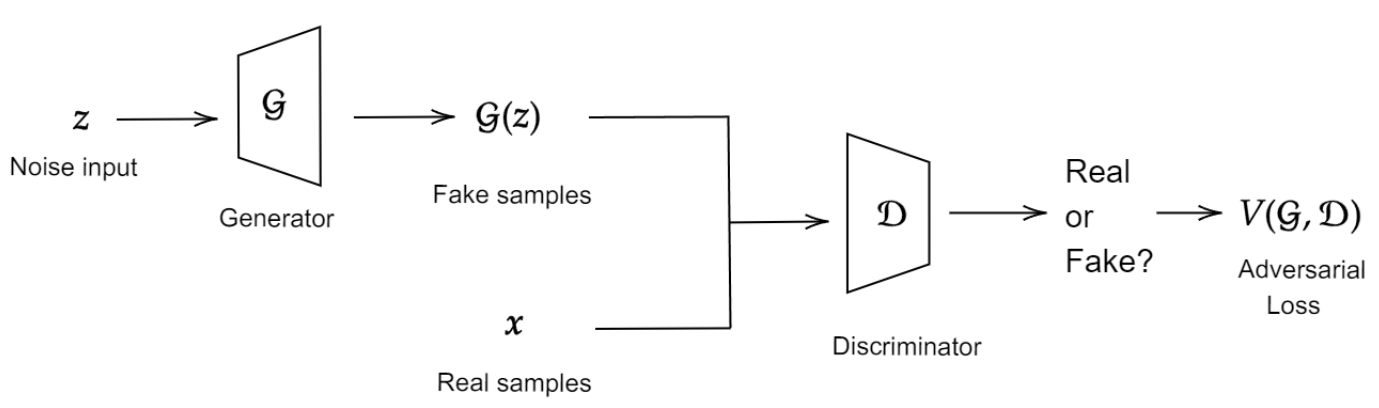
\includegraphics[width = 0.9\textwidth]{Figures/LR/GAN-schematics.png}
    \caption{Schematic diagram of vanilla GAN architecture}
    \label{GAN-schematic}
\end{figure}


\section{Kernel-based learning}
\label{sec-kernelbasedlearning}
Kernel methods were first introduced by Vapnik (1995), gaining great attention through their successful application onto Support Vector Machines (SVMs) \cite{vapnikNatureStatisticalLearning2000,cortesSupportvectorNetworks1995}. Kernel-based learning extends traditional linear approaches to non-linear scenarios by projecting input data into a high-dimensional feature space using a non-linear mapping function $\varphi(.)$. The core motivation behind that is one can expect linearly separable patterns in the feature map space, thus traditional linear techniques can learn more complex patterns from non-linear data after feature mapping. One great challenge is that features may lie in very high dimensions, possibly infinite, which makes computing $\varphi(.)$ very expensive or even intractable. 

Thanks to Mercer's theorem, it is possible to implement kernel methods without explicitly knowing the form of $\varphi(.)$ making them both powerful and computationally convenient. More precisely, given input data $\{\bx_i\}_{i=1}^{N}$ with $\bx \in \bbR^d$, Mercer's theorem states that there exists a feature mapping $\varphi: \bbR^d\to \caH$ and a kernel function $K: \bbR^d \times \bbR^d \to \bbR$ such that 
\begin{equation}
    K(\bx,\bz) = \varphi(\bx)^\top\varphi(\bz),
\end{equation}
if and only if $K(.,.)$ is a positive-definite function \cite{suykensLeastSquaresSupport2002}. The above theorem implies that kernel $K$ can be written as the dot product of two data points, and the collection of kernels on all pairs of training examples in the data set is defined as the kernel matrix (or Gram matrix) where 
\begin{equation}
\bK = \begin{bmatrix}
K(\bx_1, \bx_1) & K(\bx_1, \bx_2) & \cdots & K(\bx_1, \bx_N) \\
K(\bx_2, \bx_1) & K(\bx_2, \bx_2) & \cdots & K(\bx_2, \bx_N) \\
\vdots & \vdots & \ddots & \vdots \\
K(\bx_N, \bx_1) & K(\bx_N, \bx_2) & \cdots & K(\bx_N, \bx_N)
\end{bmatrix}.
\end{equation}
The computational problem can be then addressed by pre-computing the kernel matrix since the size of the kernel matrix is fixed on $N\times N$.
The general procedure of working on kernel matrix $\bK$ is usually referred to as \emph{kernel trick}.

Some representative applications of kernel methods in machine learning include Support Vector Machines (SVMs) \cite{cortesSupportvectorNetworks1995}, spectral clustering \cite{ngSpectralClusteringAnalysis2001}, Kernel Principal Component Analysis (KPCA) \cite{scholkopfKernelPrincipalComponent1997}, Gaussian Processes \cite{rasmussenGaussianProcessesMachine2004}, and etc. Beyond that, inspired by the powerful representation learning capabilities of deep learning architectures, there is growing interest in finding new synergies between traditional kernel methods and deep neural networks \cite{choKernelMethodsDeep2009, chenOverviewDeepKernel2016}. One notable example is Deep Restricted Kernel Machines (DRKM), which encapsulates KPCA, SVMs and possibly some other kernel learning techniques into one unified deep learning architecture via conjugate feature duality \cite{suykensDeepRestrictedKernel2017}. One can refer to \cite{hofmannKernelMethodsMachine2008,scholkopfLearningKernelsSupport2018}  for more detailed overviews and explanations on kernel-based learning.



\section{Theoretical framework of Generative restricted kernel machine}
\label{sec-tfgenrkm}
The theoretical framework of Generative restricted kernel machine (Gen-RKM) algorithm is discussed in this section. Starting by reviewing PCA and KPCA in subsection \ref{subsec-pcakpca}, the general restricted kernel machine (RKM) framework is then illustrated in subsection \ref{subsec-basicformulaRKM}. Next, subsection \ref{subsec-basicformulaGenRKM} showcases the basic training and generation algorithm of Gen-RKM under both single-view and multi-view scenarios. Besides, some related variants of Gen-RKM are introduced in subsection \ref{subsec-relatedvariantsofgenrkm}.

\subsection{A brief overviews on PCA and Kernel PCA}
\label{subsec-pcakpca}
\textbf{Basic formulation of PCA} \ Principal Component Analysis (PCA) is a widely-used unsupervised algorithm for dimensionality reduction while preserving as much variability as possible in the data \cite{bishopPatternRecognitionMachine2006, karamizadehOverviewPrincipalComponent2013}. Intuitively, PCA searches for a linear transformation such that maximizes the variance of the projected data in a lower-dimensional subspace. Orthonormal vectors that span this subspace after projection is often called \emph{principal components} (PCs). In the mathematical setting, one can formulate PCA as a constrained optimization problem. Consider a data matrix $\mathbf{X} = [\bx_1,\bx_2,\dots,\bx_N]\in \bbR^{d\times N}$ (here we assume data has already been centered for simplicity), the \emph{maximum variance formulation} \cite{bishopPatternRecognitionMachine2006} of PCA is given by 
\begin{equation}
    \begin{aligned}
        \max_{\bu_i} & \quad \bu_i^\top \mathbf{C} \bu_i \\
        \text{s.t}& \quad  \|\bu_i\|_2^2=\bu_i^\top \bu_i = 1,
    \end{aligned}
\end{equation}
where $\bu_i \in \bbR^d$ is the $i^{th}$ principal component and $\mathbf{C}$ is the sample covariance of the data ,defined as 
\begin{equation}
  \mathbf{C} = \frac{1}{N} \mathbf{X}\mathbf{X}^\top = \frac{1}{N} \sum_{n=1}^{N} \bx_{n}\bx_{n}^\top.
\end{equation}
Solving the Karush-Kuhn-Tucker (KKT) conditions of this constrained optimization problem, one can obtain the optimal conditions as the eigen-decomposition form on covariance matrix $\mathbf{C}$:
\begin{equation}
    \mathbf{C}\bu_i = \lambda_i\bu_i, \quad i=1,\dots, r.
    \label{PCA-solution}
\end{equation}
where $\lambda_i$ corresponds to the Lagrange multiplier. That indicates that the optimal principal components are the eigenvectors corresponding to the $r$ largest eigenvalues $\lambda_1, \dots, \lambda_r$ solved from eigen-decomposition problem. An alternative formulation of PCA is based on \emph{minimum reconstruction error} \cite{bishopPatternRecognitionMachine2006}. We denote a set of orthonormal directions as matrix $\mathbf{U} = [\bu_1,\bu_2, \dots, \bu_r]$, the reconstructed data point in PCA is simply $\tilde{\bx}_n = \mathbf{U}\mathbf{U}^{\top}\bx_n$, which leads to the following straightforward reconstruction error minimization problem:
\begin{equation}
    \begin{aligned}
        \min_{\mathbf{U}} & \quad \frac{1}{N}\sum_{n=1}^{N}\|\bx_n-\tilde{\bx}_n \|^2_2 \\
        \text{s.t}& \quad \mathbf{U}^\top \mathbf{U} = \mathbf{I}.
    \end{aligned}
    \label{PCA-recon-obj}
\end{equation}
It is easy to verify that the optimal solution for \ref{PCA-recon-obj} is equivalent to \ref{PCA-solution}. 

\noindent\textbf{Basic formulation of Kernel PCA} \ PCA is limited in only capturing the linear patterns in the data which makes it fail to generalize well on more complex non-linear data. Sch\"{o}lkopf et al. \cite{scholkopfKernelPrincipalComponent1997} extended the vanilla PCA algorithm to a non-linear setting based on kernel methods. Consider a non-linear mapping function $\bphi(.): \bbR^d\to \mathcal{H}$, the basic idea of kernel principal component analysis (KPCA) is to perform conventional PCA on the mapped data in the feature space. The sample covariance matrix after feature map now becomes 
\begin{equation}
    \mathbf{C}_{\bphi} = \frac{1}{N} \sum_{n=1}^{N} \bphi(\bx_{n})\bphi(\bx_{n})^\top = \frac{1}{N} \bPhi \bPhi^\top,
    \label{KPCA-eigen-decop}
\end{equation}
and its corresponding eigen-decomposition problem is given by
\begin{equation}
 \mathbf{C}_{\bphi}\bu_i = \lambda_i\bu_i, \quad i=1,\dots, r.
\end{equation}
where $\bPhi = [\bphi(\bx_1),\bphi(\bx_2),\dots,\bphi(\bx_N)]$. We usually refer to the formulation of eigen-decomposition on covariance matrix as the \emph{primal} form because function $\bphi(.)$ needs to be explicitly defined under this case. To avoid directly working on explicit feature map function $\bphi(.)$, Sch\"{o}lkopf et al. reformulated this problem by cleverly using integral operator kernel functions \cite{scholkopfKernelPrincipalComponent1997}. Starting from equation (\ref{KPCA-eigen-decop}), an equivalent form can be achieved by multiplying $\bphi(\bx_l)^\top (l = 1,\dots,N)$ on both sides : 
\begin{equation}
    \bphi(\bx_l)^\top\cdot \frac{1}{N} \sum_{n=1}^{N} \bphi(\bx_{n})\bphi(\bx_{n})^\top\bu_i = \lambda_i(\bphi(\bx_l)^\top\cdot\bu_i).
    \label{KPCA-dual-init}
\end{equation}
Moreover, one can write the eigen-vectors $\bu_i$ in the form of linear combination of $\bphi(\bx)$ where
\begin{equation}
    \bu_i = \sum_{m=1}^N h_{im}\bphi(\bx_m).
    \label{KPCA-lc-pc}
\end{equation}
Combining equations (\ref{KPCA-lc-pc}) with (\ref{KPCA-dual-init}), the key eigenvector equation can be expressed in terms of kernel function $K(\bx_i,\bx_j) = \bphi(\bx_i)\top \bphi(\bx_j)$ : 
\begin{equation}
    \frac{1}{N} \sum_{n=1}^{N} K(\bx_l,\bx_n) \sum_{m=1}^{N} h_{im} K(\bx_n,\bx_m) = \lambda_i \sum_{m=1}^{N} h_{im} K(\bx_l,\bx_n).
\end{equation}
After simplifying, one can obtain a neat expression 
\begin{equation}
    \bK\bh_i = \lambda_i N \bh_i
    \label{KPCA-dual-obj}
\end{equation}
where coefficients vector $\bh_i = [h_{i1},h_{i2},\dots, h_{im}]^\top$ and $\bK$ is the gram matrix of kernel function $K(.,.)$. It is obvious that equation (\ref{KPCA-dual-init}) is exactly the eigen-decomposition problem on kernel matrix $\bK$, hence one can solve the KPCA problem given a high dimensional feature space without demanding computational costs. Notice that when a linear kernel function is provided, KPCA will be reduced to conventional PCA.

\noindent\textbf{LS-SVM formulation of Kernel PCA} \ Least Squares Support Vector Machine (LS-SVM) is a modification on the formulation of the original SVM optimization problem introduced by Suykens et al. \cite{suykensLeastSquaresSupport1999,suykensLeastSquaresSupport2002}. The key difference between LS-SVM formulation and basic SVM formulation is in two-fold. First, inequality constraints in SVM is translated to equality constraints by introducing an error variable $\be_i$. Secondly, a squared loss term on $\be_i$ is included in the objective converting quadratic programming (QP) problem to solving a set of linear equations \cite{suykensLeastSquaresSupport2002}. The computation is greatly simplified thanks to LS-SVM form while most of key advantages of traditional SVM are preserved,  such as the primal-dual representation \cite{suykensPrimalDualModel2010}. 

Not limited to SVM classifiers, LS-SVM also provides an alternative formulation for KPCA that can be written as
\begin{equation}
    \begin{aligned}
            \min_{\mathbf{W}, \be_i}& \quad \frac{\eta}{2}\bW^\top\bW - \frac{1}{2}\sum_{i=1}^{N}\be_{i}^\top \Lambda^{-1} \be_{i}  \\
    \text{s.t}& \quad \be_i = \bW^\top \bphi(\bx_i) \quad \forall i =1,\dots,N
    \label{LSSVM-KPCA-OBJ}
    \end{aligned}
\end{equation}
with $\Lambda = \text{diag}(\lambda_1,\dots,\lambda_r)$ and transformation matrix $\bW$. This optimization problem is analogous to one class modeling problem in the context of SVM where only a zero target value is considered. One can recover the optimal solution to the eigen-problem on kernel matrix $\bK$ (equation (\ref{KPCA-dual-obj})) by solving the KKT conditions. In case $\bphi(\bx)$ is not zero-mean, centering before performing PCA is nontrivial. The error variable (or score variable) in problem (\ref{LSSVM-KPCA-OBJ}) then becomes $\quad \be_i = \bW^\top (\bphi(\bx_i) - \boldsymbol{\mu_{\bphi}})$ \cite{suykensLeastSquaresSupport2002}.


\noindent\textbf{Preimage problem in Kernel PCA} \ One important use case in KPCA is denoising, i.e. removing unwanted noisy patterns by projecting training data onto subspace spanned by eigenvectors. Furthermore, denoising requires mapping the projected data back to the original input space, namely reconstructing the data. Reconstruction in linear PCA is straightforward because only simple matrix multiplication is involved. However, reconstructing data in Kernel PCA is way more complicated due to the implicit nature of feature map function $\bphi(.)$, no exact solution exists for reversing the feature map. The general challenge of approximating the reconstructed data in kernel-based algorithms is known as \emph{pre-image} problem \cite{honeinePreimageProblemKernelBased2011, mikaKernelPCADeNoising1998a}. To tackle this problem, various approaches have been proposed in the last few decades, including fixed-point iterations \cite{mikaKernelPCADeNoising1998a}, multidimensional scaling-based techniques \cite{kwokPreimageProblemKernel2004a}, and many others.

\subsection{Basic formulation of RKM}
\label{subsec-basicformulaRKM}
Suykens further extended LS-SVM formulations of different kernel machines to the framework of Restricted Kernel Machine (RKM), allowing a more intuitive architecture with visible-hidden unit representations \cite{suykensDeepRestrictedKernel2017}. In our work, RKM is limited to KPCA with RKM representations.

As the most fundamental building block of RKM framework, we start by introducing the conjugate feature duality.
\begin{lemma}[Conjugate feature duality] 
Given a diagonal matrix $\Lambda = \text{diag}(\lambda_1,\dots,\lambda_S)$ ,for all $ \be, \bh\in \bbR^{s}$, we have
\begin{equation}
         \frac{1}{2}\be^\top\Lambda^{-1}\be + \frac{1}{2}\bh^\top\Lambda\bh \geq \be^\top\bh.
\end{equation}
\end{lemma}

\begin{proof}
Fenchel's inequality states that for any pair of convex conjugate functions $f$ and $f^*$, the following inequality holds:
\begin{equation}
    f(x) + f^{*}(y) \geq x^\top y
\end{equation}
where the definition of conjugate function on $f(x)$ is given by $f^{*}(y) = \sup _{x} (y^\top x - f(x))$ \cite{boydConvexOptimization2004}. We define the following function  
\begin{equation}
    f(\be) = \frac{1}{2}\be^\top \Lambda^{-1} \be
\end{equation}
with its corresponding convex conjugate
\begin{equation}
    f^{*}(\bh) = \sup_{\be} (\be^\top\bh - \frac{1}{2}\be^\top\Lambda^{-1}\be).
\end{equation}
To find the supremum, we compute the stationary points of $f^{*}(\bh)$ with respect to $\be$ : 
\begin{equation}
    \begin{aligned}
    \frac{\partial}{\partial \be} (\be^\top\bh - \frac{1}{2}\be^\top\Lambda^{-1}\be) &= \bh - \Lambda^{-1}\be = 0 \\
    \be = \Lambda\bh.
    \end{aligned}
\end{equation}
Substituting $\be = \Lambda\bh$ back into $f^{*}(\bh)$:
\begin{equation}
    \begin{aligned}
        f^{*}(\bh) & = (\Lambda\bh)^\top\bh - \frac{1}{2}(\Lambda\bh)^\top\Lambda^{-1}(\Lambda\bh) \\
        &= \frac{1}{2}\bh^\top \Lambda\bh.
    \end{aligned}
\end{equation}
Conjugate feature duality can be justified if we apply Fenchel-Young inequality:
\begin{equation}
    \begin{aligned}
        f(\be) + f^*(\bh) &\geq \be^\top \bh \\
         \frac{1}{2}\be^\top\Lambda^{-1}\be + \frac{1}{2}\bh^\top\Lambda\bh &\geq \be^\top\bh.
    \end{aligned}
\end{equation}
\end{proof}
$\bh$ can be viewed as hidden units in the RKM framework. One can then deduce an upper bound of the LS-SVM objective by replacing the squared loss term on $\be$, while new hidden units are introduced and optimality conditions remain unchanged. Suykens refers to the general process of introducing hidden units via the above inequality as \emph{conjugate feature duality}.

\noindent\textbf{Kernel PCA under the framework of RKM} \ We now investigate the RKM representation of KPCA. Applying the conjugate feature duality on the objective of LS-SVM formulation of KPCA (equation \ref{LSSVM-KPCA-OBJ}), we will achieve the training objective function of RKM:
\begin{equation}
    \begin{aligned}
        \caJ_{\text{KPCA}} &= \frac{\eta}{2}\bW^\top\bW - \frac{1}{2}\sum_{i=1}^{N}\be_{i}^\top \Lambda^{-1} \be_{i} \quad (\text{s.t.} \ \be_i = \bW^\top \bphi(\bx_i))  \\
& \leq -\sum_{i=1}^{N}\bphi(\bx_i)^\top\bW\bh_i + \frac{1}{2}\sum_{i=1}^{N}\bh_i^\top\Lambda\bh_i + \frac{\eta}{2}\bW^\top\bW = \caJ_{\text{RKM}}.
\label{RKM-KPCA-OBJ}
    \end{aligned}
\end{equation}
Stationary points of $\caJ_{\text{RKM}}$ is characterized by
\begin{equation}
    \begin{cases}
    \displaystyle
\frac{\partial \mathcal{J}_\text{RKM}}{\partial \bh_i} = 0 \implies \Lambda \bh_i = \bW^\top \bphi(\bx_i), \quad \forall i \\
    \displaystyle
    \frac{\partial \mathcal{J}_\text{RKM}}{\partial \bW} = 0 \implies \bW = \frac{1}{\eta} \sum_{i=1}^N \bphi(\bx_i) \bh_i^\top. \\
\end{cases}
\end{equation}
By eliminating either variable $\bh_i$ or $\bW$, one can arrive at different eigen-decomposition problems corresponding to primal-dual representation :
\begin{equation}
    \begin{cases}
        \displaystyle
    \text{Eliminating $\bh_i$} \implies \quad \frac{1}{\eta}\bK\bH^\top = \bH^\top\Lambda \quad \text{(Dual)}  \\
    \displaystyle
    \text{Eliminating $\bW$} \implies \quad \frac{1}{\eta}\bS_{\bPhi}\bW = \Lambda\bW  \quad \text{(Primal)}
    \end{cases}
    \label{RKM-KPCA-primal-dual}
\end{equation}
where matrix $\bH = [\bh_1,\dots,\bh_N]$ is the collection of all latent variables and matrix $\bS_{\bPhi} = \bPhi\bPhi^{\top}$ is proportional to the sample covariance matrix. 

\noindent\textbf{Connections with RBM} \ Restricted Boltzmann Machine (RBM) is a type of energy-based stochastic neural network, consisting of visible and hidden units as the basic building blocks \cite{zhangOverviewRestrictedBoltzmann2018, fischerIntroductionRestrictedBoltzmann2012}. The key difference between RBM and general BM is that there is no direct connections between units within the same layer, i.e. no interconnections within the group of visible units or hidden units. Computation in RBM is relatively more efficient thanks to this restriction. Denote the set of (binary) visible variables as $\bv \in \{0,1\}^{d}$ and the set of (binary) hidden variables of $\bh \in \{0,1\}^{s}$, the energy function of RBM is given by
\begin{equation}
    \caJ_{\text{RBM}}(\bv,\bh) = -\bv^{\top}\bW\bh - \bc^{\top}\bv - \ba^{\top}\bh
\end{equation}
where $\bW$ acts as the weighting matrix (or interconnection matrix) from layer to layer and $\bc$, $\ba$ are the bias terms. The joint distribution function of RBM  is obtained by normalizing the exponential of the negative energy function :
\begin{equation}
    p(\bv,\bh) = \frac{1}{Z(\bv,\bh)} \exp{(-\caJ_{\text{RBM}}(\bv,\bh))}.
\end{equation}
The normalization term is often known as \emph{partition function} which is given by $Z(\bv,\bh) = \sum_{\bv}\sum_{\bh}\exp{(-\caJ_{\text{RBM}}(\bv,\bh))}$. If comparing the above energy function with the training objective in RKM (equation (\ref{RKM-KPCA-OBJ})), one can observe that the interaction term $-\bv^{\top}\bW\bh$ appears in both RKM and RBM objective, capturing how the states of the visible units influence the states of the hidden units and vice versa. Apart from a similar energy function form, the notation "R" in "RKM" also refers to no hidden-to-hidden or visible-to-visible interconnections existing in the model architecture. There are also some key differences between RBM and RKM. First, units in RBM are typically binary-valued, while RKM models the underlying patterns within real-valued variables. Although there exist several works \cite{hintonFastLearningAlgorithm2006, wangAnalysisGaussianbinaryRestricted2012, ranzatoFactored3WayRestricted2010} that attempt to generalize classical RBM to modeling real-valued distribution, difficulty in training and inference is still a big issue \cite{wangAnalysisGaussianbinaryRestricted2012}. Second, training in RKM is based on minimizing the empirical loss using a classical gradient descent approach, whereas RBM tends to maximize the likelihood via k-step contrastive divergence (CD-k) algorithm \cite{carreira-perpinanContrastiveDivergenceLearning2005}.

\noindent\textbf{Deep RKM} \ RKM is not limited to a single-layer architecture; multiple RKMs can be coupled using the property of conjugate feature duality to form a unified deep architecture \cite{suykensDeepRestrictedKernel2017}. More specifically, consider the KPCA training objective under RKM framework in layer $l$:
\begin{equation}
    \caJ_{\text{RKM}_l} = -\sum_{i=1}^{N} \bphi_{l}(\bh_i^{(l-1)})^\top \bW_{l} \bh_i^{(l)} + \frac{1}{2} \sum_{i=1}^{N} \bh_i^{(l)\top} \Lambda_{l} \bh_i^{(l)} + \frac{\eta}{2} \bW_{l}^\top \bW_{l}.
\end{equation}
The training objective for coupled KPCAs is then given by simply summation of objectives from different layers:
\begin{equation}
    \caJ_{\text{DRKM}} = \sum_{l=1}^{L} \caJ_{\text{RKM}_l}.
\end{equation}
The input of each layer is the output of the previous layer (i.e. latent variables yielded by previous KPCA operation), notice that $\bh^{(0)}$ refers to the original training data for the starting layer. Based on the framework of DRKM, Tonin et al. \cite{toninUnsupervisedLearningDisentangled2021} introduced orthogonality constraints on the latent variables to encourage disentanglement as well as to simplify the optimization process. The general theoretical framework of the deep KPCA methodology is summarized in \cite{toninDeepKernelPrincipal2024}. Furthermore, recent studies \cite{toninDeepKernelPrincipal2024} have empirically shown that deep KPCA can achieve better disentanglement capability compared to the state-of-the-art InfoVAE \cite{zhaoInfoVAEBalancingLearning2019} due to its effective hierarchical learning process.

\subsection{Basic formulation of Generative RKM}
\label{subsec-basicformulaGenRKM}
\noindent\textbf{Generative kernel PCA} \ Schreurs and Suykens \cite{schreursGenerativeKernelPCA2018} proposed a generative version of KPCA, by defining the following generation objective function:
\begin{equation} 
    \caJ_{\text{KPCA-gen}} = -\bphi(\bx^{*})^\top\widehat{\bW}\bh^{*} + \frac{1}{2}\bphi(\bx^*)^{\top}\bphi(\bx^*)
\end{equation}
with a new generated data point $\bx^{*}$ and its corresponding hidden variable $\bh^{*}$. The estimated interconnection matrix from the training phase is denoted by $\widehat{\bW}$. By solving the stationary point, one can show the generated data is given by the equation:
\begin{equation}
\frac{\partial\caJ_{\text{KPCA-gen}}}{\partial \bphi(\bx^{*})} = 0 \implies \bphi(\bx^{*}) = \widehat{\bW}\bh^{*} = (\frac{1}{\eta}\sum_{i=1}^{N}\bphi(\bx_i)\bh_i^\top)\bh^{*}.
\end{equation}
New $\bh^{*}$ is randomly sampled from a fitted Gaussian distribution on the trained hidden units. Then a natural question arises: how to tackle the pre-image problem, i.e. how to recover $\bx^{*}$ from the form $\bphi(\bx^*)$ when feature map function is implicitly defined? As mentioned in the previous section, the exact solution may not exist due to the implicit nature of $\bphi(.)$. Schreurs and Suykens \cite{schreursGenerativeKernelPCA2018} showed a possible solution by implementing kernel smoothing approach. Through 
multiplying any training data point after feature map $\bphi(\bx_j)^{\top} \text{for }\forall j\in \{1,\dots,N\}$, one can obtain the following relation:
\begin{equation}
    \bk_{\bx^*} = \frac{1}{\eta}\bK\bH^\top\bh^*
\end{equation}
where $\bk_{\bx^*} = [K(\bx_1,\bx^*),\dots,K(\bx_N,\bx^*)]^\top$ is a collection of similarity measures between new data point and remaining training data points in the feature space. The estimation of $\bx^*$ from kernel smoothing is given by
\begin{equation}
    \hat{\bx}^* = \frac{\sum_{j=1}^{N_r}\Tilde{K}(\bx_j,\bx^*)\bx_j}{\sum_{j=1}^{N_r}\Tilde{K}(\bx_j,\bx^*)}
\end{equation}
where $\Tilde{K}(.,.)$ refers to the scaled version of similarity measures and $N_r < N$ needs to be specified beforehand indicating the number of closest (or most similar) points based on the kernel function.

\noindent\textbf{Generative RKM} \ Pandey et al. \cite{pandeyGenerativeRestrictedKernel2021} introduced a novel framework for generative learning, combining KPCA with deep neural network architectures.  To address the pre-image problem, they implemented an alternative approach using a deep convolutional neural network as the feature map function, denoted by $\bphi(.)$ and parameterized by $\boldsymbol{\theta}$. Additionally, another convolutional neural network $\bpsi(.)$, typically the inversion of the neural network used in the feature map, parameterized by $\boldsymbol{\zeta}$, is employed as the pre-image map. An intuitive link between autoencoders and Gen-RKM emerges when considering the feature map as the encoder part and the pre-image map as the decoder part, that is Gen-RKM can be viewed as an autoencoder with Kernel PCA in the bottleneck layer. In this specific architecture, disentanglement is encouraged thanks to the mutually uncorrelated eigenvectors from KPCA operation.

During the training phase, the network parameters are updated in a mini-batching scheme by jointly minimizing the reconstruction errors and objective for KPCA. More specifically, the training objective in Gen-RKM is defined as follows:
\begin{equation}
    \begin{aligned}
 &\caJ_{\text{Gen-RKM}} = \underbrace{\caJ_{\text{RKM}} + \frac{c_{\text{stab}}}{2}\caJ_{\text{RKM}}^2}_{\text{stabilization}} + \underbrace{\frac{\gamma}
        {N}\caJ_{\text{recon}}}_{\text{reconstruction error}} \\
        \text{s.t.}\quad & \caJ_{\text{recon}} = \sum_{i=1}^{N}\|\bx_i - \bpsi(\bphi(\bx_i)) \|_2^2.
    \end{aligned}
    \label{Gen-RKM-stab-obj}
\end{equation}
Notice that a stabilized version of the training objective on KPCA is employed in practice since the minus sign term will possibly lead to loss explosion as suggested by Sukyens \cite{suykensDeepRestrictedKernel2017}. Pandey et al. \cite{pandeyGenerativeRestrictedKernel2021} have proved that the optimality conditions remain unchanged under this transformation. The constants $c_{\text{stab}}$ and $\gamma$ act as the regularization parameters in the training objective. The final optimization problem is then given by
\begin{equation}
    \min_{(\boldsymbol{\theta},\boldsymbol{\zeta})} \caJ_{\text{Gen-RKM}}.
\end{equation}

The generation phase in Gen-RKM is basically the same as in KPCA. The only difference is that we first fit a Gaussian mixture model (GMM) over the all trained latent representations, a new latent variable is then randomly sampled from the fitted GMM model. Since feature map and pre-image map is explicitly defined by neural network models, corresponding generated data can be obtained via simple matrix multiplication without effort. 

The detailed training and generation algorithm for Gen-RKM is depicted in algorithm \ref{alg-gen-rkm-dual}. Notice that a final computation step is implemented in practice, performing SVD on the full kernel matrix to get all latent variables and weighting matrix. This step can be highly computationally expensive under the dual form when $N$ (number of data points) is very large since the time complexity of SVD is $\mathcal{O}(N^3)$. Thanks to the primal-dual representation of RKM framework, one can address this issue by solving the KPCA problem in the primal form (eigen-decomposition on $\bS_{\bPhi}$, see equation (\ref{RKM-KPCA-primal-dual})). The size of covariance matrix $\bS_{\bPhi}$ is fixed on $d_f\times d_f$, where the dimension of feature space $d_f$ is typically way smaller than $N$, and computation on all latent variables $\bH$ just involves simple matrix multiplication. Hence one can choose to perform Gen-RKM algorithm in either primal or dual form depending on different $N$ and $d_f$, ensuring the scalability of Gen-RKM to large-scale dataset \cite{pandeyGenerativeRestrictedKernel2021, achtenDualityMultiViewRestricted2023}.
\begin{algorithm}[H]
\caption{Training and generation algorithm for one-view Gen-RKM (Dual) \cite{pandeyGenerativeRestrictedKernel2021}}
\label{alg-gen-rkm-dual}
\begin{algorithmic}[1]
\Require training data $\{\bx_i\}_{i=1}^{N}$; mini-batch size $m$; \\
regularization parameters $\eta, c_{\text{stab}}, \gamma$; \\
explicit feature map $\bphi_{\boldsymbol{\theta}}(.)$ and explicit pre-image map $\bpsi_{\boldsymbol{\zeta}}(.)$; \\
dimension of latent space $s$ and number of components for fitting GMM $l$;
\Procedure{Training}{}
\LComment{Training loop}
    \For{each epoch}
        \For{each mini-batch}
        \State Get mini-batch $\{\bx_i\}_{i\in B}$ with $B \subset\{1,\dots,N\}$ via uniform sampling
        \State $\bPhi \gets \bphi_{\boldsymbol{\theta}}(\{\bx_i\}_{i\in B})$ 
        \State $\bK \gets \bPhi^\top\bPhi$
        \State $\bH,\Lambda \gets \text{SVD}(\bK)$ \Comment{Eigen-decomposition on kernel matrix}
        \State $\bW\gets \bPhi\bH^\top$
        \State $\widehat{\bPhi} \gets \bW \bH$
        \State update $\{\boldsymbol{\theta},\boldsymbol{\zeta}\} \gets \text{Adam}(\caJ_\text{Gen-RKM})$ \Comment{Update network parameters}
        \EndFor
    \EndFor
\LComment{Final computation step to get all latent variables on full dataset}
\State $\bPhi_{\text{full}} \gets \bphi_{\boldsymbol{\theta}}(\{\bx_i\}_{i=1}^{N})$
\State repeat step 7-9 on $\bPhi_{\text{full}}$
\EndProcedure
\Procedure{Generation}{}
\State $p(\bh) \gets \text{GMM}_{l}(\bH)$
\State $\bh^* \sim p(\bh)$  \Comment{Random sampling from the fitted GMM}
\State $\bx_{\text{gen}} \gets \bpsi_{\boldsymbol{\zeta}}(\bW \bh^{*})$
\EndProcedure

\end{algorithmic}
\end{algorithm}

\noindent\textbf{Extensions to multi-view learning in Gen-RKM} \ Now we consider the generalized form of Gen-RKM with extension to multi-view learning. \emph{Views} generally refers to different data representations (or modalities), and multi-view learning corresponds to the unified modeling process to learn the common feature spaces or shared underlying pattern from different data sources \cite{yanDeepMultiviewLearning2021}.  For illustration purposes, we will present the two-view setting. One can refer to \cite{achtenDualityMultiViewRestricted2023} for the theoretical formulation of a more general multi-view case.

Specifically, given a training dataset with two views : $\{\bx_i,\by_i\}_{i=1}^{N}$ where $\bx_i \in \bbR^d$ and $\by_i\in \bbR^p$ (one can view $\{\bx_i,\by_i\}$ as a feature-label pair). The training objective for two-view data in KPCA under RKM form can be formulated as
\begin{equation}
    \begin{aligned}
    \caJ_{\text{RKM-MV}} = &- \sum_{i=1}^{N} \bphi_{\bx}(\bx_i)^\top \bW_{\bx} \bh_i 
    - \sum_{i=1}^{N} \bphi_{\by}(\by_i)^\top \bW_{\by} \bh_i \\
    &+ \frac{1}{2} \sum_{i=1}^{N} \bh_i^\top \Lambda \bh_i 
    + \frac{\eta_{\bx}}{2} \bW_{\bx}^{\top} \bW_{\bx} 
    + \frac{\eta_{\by}}{2} \bW_{\by}^{\top} \bW_{\by}
    \end{aligned}
\end{equation}
where the feature map function for each view is denoted by $\bphi_{\bx}(.): \bbR^d\to \caH_{\bx}$ and $\bphi_{\by}(.): \bbR^d\to \caH_{\by}$
respectively. $\bW_{\bx}\in \bbR^{d_f \times s}$ and $\bW_{\by} \in \bbR^{p_f\times s}$ are the interconnection matrices corresponding to each view where $d_f, p_f$ are the dimensions of feature spaces and $s$ indicates the dimension of latent space (number of selected principal components from KPCA). Likewise, with the one-view setting, different eigenvalue problems associated with primal-dual representations can be obtained by solving the stationary points of $\caJ_{\text{RKM-MV}}$: 
\begin{equation}
    \begin{cases}
        \displaystyle
        [\frac{1}{\eta_{\bx}}\bK_{\bx} + \frac{1}{\eta_{\by}}\bK_{\by}]\bH^\top = \bH^\top\Lambda \quad \text{(Dual)} \\
        \\
        \begin{bmatrix}
        \frac{1}{\eta_{\bx}} \bPhi_{\bx} \bPhi_{\bx}^\top & \frac{1}{\eta_{\bx}} \bPhi_{\bx} \bPhi_{\by}^\top \\
        \frac{1}{\eta_{\by}} \bPhi_{\by} \bPhi_{\bx}^\top & \frac{1}{\eta_{\by}} \bPhi_{\by} \bPhi_{\by}^\top
        \end{bmatrix}
        \begin{bmatrix}
        \bW_{\bx} \\
        \bW_{\by}
        \end{bmatrix}
        =
        \begin{bmatrix}
        \bW_{\bx} \\
        \bW_{\by}
        \end{bmatrix}
        \Lambda \quad \text{(Primal)}.   
    \end{cases}
\end{equation}
One can see that the dual form is the eigen-decomposition of the weighted summation of kernel matrices, while the primal form considers the general cross-covariance matrix of feature vectors from different views. Pre-image maps are also explicitly defined by two convolutional neural networks for the purpose of reconstruction. The reconstruction loss in multi-view settings is simply generalized to the summation of reconstruction errors from different views. Combining both the KPCA objective and reconstruction loss, one can employ the same stabilization trick to form the final training objective (equation (\ref{Gen-RKM-stab-obj})), and the training process stays largely the same as algorithm \ref{alg-gen-rkm-dual}.

As for the generation phase, the following generating objective is considered :
\begin{equation}
    \begin{aligned}
    \caJ_{\text{MV-RKM-gen}} = &-\bphi_{\bx}(\bx^{*})^\top\widehat{\bW}_{\bx}\bh^{*}-\bphi_{\by}(\by^{*})^\top\widehat{\bW}_{\by}\bh^{*} \\ 
    &+ \frac{1}{2}\bphi_{\bx}(\bx^*)^{\top}\bphi_{\bx}(\bx^*)+ \frac{1}{2}\bphi_{\by}(\by^*)^{\top}\bphi_{\by}(\by^*).
    \end{aligned}
\end{equation}
Different views of data share one common latent variable in the multi-view setting. Once $\bh^{*}$ is sampled from the trained GMM, generated data under feature spaces is given by
\begin{equation}
    \begin{aligned}
        \bphi_{\bx}(\bx^{*}) &= \widehat{\bW}_{\bx}\bh^{*} \\
         \bphi_{\by}(\bx^{*}) &= \widehat{\bW}_{\by}\bh^{*},
    \end{aligned}
\end{equation}
which can be readily reversed back to input data space via explicit pre-image map likewise in the single-view setting.

\subsection{Related variants of Generative RKM}
\label{subsec-relatedvariantsofgenrkm}
\noindent\textbf{Stiefel RKM} \ Generative RKM requires performing exact SVD at each iteration which could possibly cause numerical instability during the backpropagation process. Moreover, training Gen-RKM can be rather computationally demanding when both mini-batch size and feature space dimension are large. Pandey et al. \cite{pandeyDisentangledRepresentationLearning2022} proposed a modified version of Gen-RKM, namely Stiefel RKM, to address these limitations. The training objective for Stiefel RKM is restated as
\begin{equation}
    \begin{aligned}
        \min_{\bU,(\btheta,\bzeta)} \caJ_{\text{St-RKM}} = &\underbrace{\frac{\lambda}{N}\sum_{i=1}^{N}\|\bx_i - \bpsi_{\bzeta}(\bU\bU^\top\bphi_{\btheta}(\bx_i)) \|^2_2}_{\text{encoder-decoder reconstruction}}  \\
        & + \underbrace{\frac{1}{N}\sum_{i=1}^{N}\| \bphi_{\btheta}(\bx_i) - \bU\bU^{\top}\bphi_{\btheta}(\bx_i) \|_2^2}_{\text{KPCA reconstruction}} \\
        \text{s.t.} \quad & \bU^\top \bU = \mathbf{I},
    \end{aligned}
\end{equation}
where the constraint set enforcing the orthogonality of the matrix is called as \emph{Stiefel manifold} \cite{tagareNotesOptimizationStiefel2011}. In the training phase, transformation matrix $\bU$ and network parameters $(\btheta,\bzeta)$ are jointly optimized in each iteration. Cayley-Adam algorithm \cite{liEfficientRiemannianOptimization2020} is implemented for optimizing the KPCA reconstruction objection, while the autoencoder objective is minimized via the classical Adam optimizer. This approach avoids the expensive computation of exact SVD during the training process.

\noindent\textbf{Robust RKM} \ Pandey et al. \cite{pandeyRobustGenerativeRestricted2020} observed that Gen-RKM could be sensitive to the outliers in the training data. A weighting scheme is incorporated with the Gen-RKM framework to combat unwanted bias caused by contamination in the training data as well as impose additional regularization on the loss objective. Assuming a positive-definite diagonal weighting matrix $\bD = \text{diag}(d_1,\dots,d_N)$, the training objective for weighted RKM is defined as
\begin{equation}
    \begin{aligned}
        \caJ_{\text{WRKM}} = -\sum_{i=1}^{N}\bphi_{\btheta}(\bx_i)^\top\bW\bh_i + \frac{1}{2}\sum_{i=1}^{N}\bD_{ii}^{-1}\bh_i^\top\Lambda\bh_i + \frac{\eta}{2}\bW^\top\bW
    \end{aligned},
\end{equation}
which corresponds to the eigen-decomposition problem on the weighted kernel matrix (if eliminating the primal variable). The final training objective of robust RKM is composed of the weighted reconstruction error and the weighted KPCA loss after employing the same stabilization trick :
\begin{equation}
    \min_{(\btheta,\bzeta)}\caJ_{\text{Rob-RKM}} = \caJ_{\text{WRKM}} + \frac{c_{\text{stab}}}{2} + \caJ_{\text{WRKM}}^2 + \frac{\gamma}{N}\bD_{ii}\caJ_{\text{recon}}.
\end{equation}
Pandey et al. \cite{pandeyRobustGenerativeRestricted2020} proposed computing weighting matrix $\bD$ based on Minimum Covariance Determinant (MCD) which is a commonly-used robust estimator against contaminated data.



\section{Learning from unbalanced data}
\label{sec-learning-from-unbalanced-data}
\subsection{Re-sampling and re-weighting technique}

Re-sampling is normally performed during the data preprocessing phase prior to training a model. It modifies the prior probability of the majority and minority class in the training set to obtain a more balanced number of instances in each class. For unbalanced data, resampling can be divided into two categories, over-sampling and under-sampling. Over-sampling methods balance input data by increasing the number of samples from the minority classes. It can be done by simply duplicating the samples from the minority classes, or more generally, manually creating new samples for the minority classes based on the existing minority samples. For instance, Chawla et al. initially introduced the widely adopted SMOTE technique \cite{Chawla_2002}. Subsequently, various modifications \cite{10.1007/11538059_91} and extensions to deep learning \cite{9694621} have been extensively explored and developed. The advantage of over-sampling is that it utilizes all information of samples in the training set. However, there is a risk that minority classes may become overrepresented in the training set, potentially leading to overfitting. Conversely, under-sampling deals with unbalanced data by dropping out samples from the majority class while preserving all the minority class samples. For example, the Random Under-Sampling(RUS) randomly eliminates the samples of the majority class\cite{tahir2009multiple}. This method is well-suited for large-scale applications where the majority classes are substantially larger. Reducing the number of training samples can decrease training time and make the learning problem more computationally tractable\cite{1549828}. However, it is risky to lose information of the samples from the majority class since informative samples may be randomly dropped out. Lima and Pereira(2015) found that instead of dropping samples, reducing the number of irrelevant features also significantly improves the model performance on unbalanced data\cite{7397461}. 

Re-weighting methods, also known as cost-sensitive based methods, are an alternative technique to deal with unbalanced data problems. Unlike the resampling which is performed during the data preprocessing phase, re-weighting works during the training phase of model construction by assigning different weights to different samples when calculating training loss. Berardi and Zhang initially proposed cost-sensitive neural networks by assigning different costs to errors in different classes\cite{berardi1999effect}. A classic empirical re-weighting method is to assign the samples of each class with the same weight, such as inverse class frequency\cite{Huang_2016_CVPR, NIPS2017_147ebe63}. It has been further explored by the class-balanced loss\cite{cuiClassBalancedLossBased2019}, which calculates the effective number of examples as class frequency. Besides these empirical re-weighting methods, there are also automatic re-weighting methods that obtain the weights using learning algorithms. Park et al. proposed influence-balanced loss to re-weight samples by the magnitude of the gradient\cite{Park_2021_ICCV}. Liu et al. also propose a method that updates the sample weights under a certain constraint\cite{liu2022improving}.

Furthermore, ensemble-based classifiers, which are known to improve the performance of a single classifier by combining several base classifiers that outperform every independent one\cite{lane2012developing, krawczyk2013improved}, can also be applied to tackle imbalanced data problems. More techniques focus on modifying the classical algorithms, such as kernel and activation function transformation method\cite{raj2016towards, wu2016mixed}, task decomposition strategies\cite{xiao2016imbalanced} and objective function transformation, are also well explored. 

\subsection{Unbalanced data in supervised and unsupervised learning}
\label{subsec-lr-unbalance-super-unsuper}
In the case of supervised learning, labeled datasets are used to train algorithms to predict outcomes and recognize patterns. The unbalanced data problem would happen when the number of training samples of the minority classes is much smaller compared to other majority classes. As a result, the trained classifiers tend to choose the majority classes and ignore the minority class by treating them as noise\cite{lu1998robust, articleM}. To deal with these problems, both resampling and cost-sensitive-based re-weighting algorithms mentioned in section 2.4.1 can be implemented. 

In unsupervised learning, the issue of unbalanced data is less clearly defined because the training data lacks labels, making it challenging to determine whether the dataset is balanced. In this case, most research efforts are concentrated on identifying distinct patterns within the majority of the data, a process often referred to as anomaly detection or outlier detection\cite{chandola2009anomaly}. Isolation Forest is an efficient anomaly detection algorithm that is similar to the Random Forest, but it chooses the splitting attribute and split point (value) randomly instead of based on information gain or Gini index. During the tree-building process, if some samples quickly reach the leaf nodes (i.e., the distance from the leaf to the root is short), they are considered likely anomalies\cite{liu2008isolation}. Besides, clustering techniques can also be used for outlier detection. For example, DBSCAN\cite{ester1996density} and local outlier factor (LOF)\cite{breunig2000lof} both consider as outliers the samples that have a substantially lower density than their neighbors. Meanwhile, one-class classification methods like SVDD \cite{tax1999support} and its extension Deep-SVDD \cite{pmlr-v80-ruff18a} provide a different approach. These methods establish spherical boundaries around samples in the feature space, aiming to minimize the volume of the hypersphere to effectively detect outlier samples. 

\subsection{Unbalanced data in generative learning}
\label{subsec-ub-gen}
From the perspective of generative models, an imbalance in training data can be detrimental because a skewed data distribution may introduce undesirable biases towards overrepresented modes. The phenomenon where generation becomes less diverse due to data imbalance is commonly referred to as mode collapse, and it has been widely studied in the context of GANs \cite{goodfellowGenerativeAdversarialNets2014}. However, the mode collapse problem in GANs is not merely specific to data imbalance; other possible causes include gradient vanishing during training, non-convergence of the adversarial loss, discriminator overpowering, and so on \cite{kossaleModeCollapseGenerative2022}. Of course, some works still exist that specifically address the issue of mode collapse in GANs under the data imbalance scenario. Mariani et al. introduce the BAGAN (Balancing GAN) methodology, through an autoencoder-based initialization strategy, which is capable of generating samples with high quality and high diverse conditioned on minority classes, even when the data is extremely imbalanced \cite{marianiBAGANDataAugmentation2018}. Huang et al. further enhance the training stability of BAGAN by introducing an additional gradient penalty term \cite{huangEnhancedBalancingGAN2023}. An alternative approach is to integrate a self-damaging contrastive learning scheme with GAN architecture, known as Damage GAN \cite{anaissiDamageGANGenerative2024}. Anaissi et al. have shown that Damage GAN is able to generate images with higher quality and greater diversity on the imbalanced training dataset compared to vanilla GAN, as indicated by lower Inception Score (IS) and Fr\'{e}chet inception distance (FID) \cite{anaissiDamageGANGenerative2024}. As for research on VAEs in the context of imbalanced data, a representative work is Jigsaw-VAE, which combats the adverse effect brought by feature imbalance by implementing a permutation-based regularization scheme \cite{asgaritaghanakiJigsawVAEBalancingFeatures2020}. For RKM-related work, to the best of our knowledge, no studies have yet discussed the data imbalance issue in RKM.






% From the perspective of generative models, an imbalance in training data can be detrimental because a skewed data distribution may introduce undesirable biases towards overrepresented modes. This imbalance often results in less diverse samples, known as mode collapse, during the generation phase. For instance, in Variational Autoencoders (VAE), training on unbalanced data can cause the model to learn biased means and standard deviations, leading to the generation of biased samples. Based on the various architectures of generative models, the resampling and reweighting methods outlined in section 2.4.1 can also be utilized to address the issue of data imbalance. For example, Schreurs et al. have successfully integrated ridge leverage score (RLS) sampling into Generative Adversarial Networks (GANs) by assigning differential weights to training samples according to their uniqueness \cite{schreursLeverageScoreSampling2022}.


 \cleardoublepage

\chapter{Problem Statement}
\label{chap-ps}
This chapter aims to get a deeper insight into the effect of data imbalance within the Gen-RKM framework. In Gen-RKM, new samples are generated by first sampling from the estimated distribution of the latent space $\mathcal{L}$. The sampled latent point is then reconstructed into image shapes via the transpose of interconnection matrix $\bW^{\top}$ and the pre-image network $\bpsi$ (shown in Figure \ref{rkm-demo}). As described in algorithm \ref{alg-gen-rkm-dual}, the latent representations of the training samples are essentially the mutually orthogonal eigenvectors yielded from KPCA. Therefore, if there is an imbalance existing in the data, the minority modes in the original training dataset would also result in corresponding minority groups in the latent space. Simply speaking, an imbalance in the input dataset would cause an imbalance in the latent space representations, resulting in a biased distribution and, ultimately, a less diverse generation. 

\begin{figure}[ht]
    \centering
    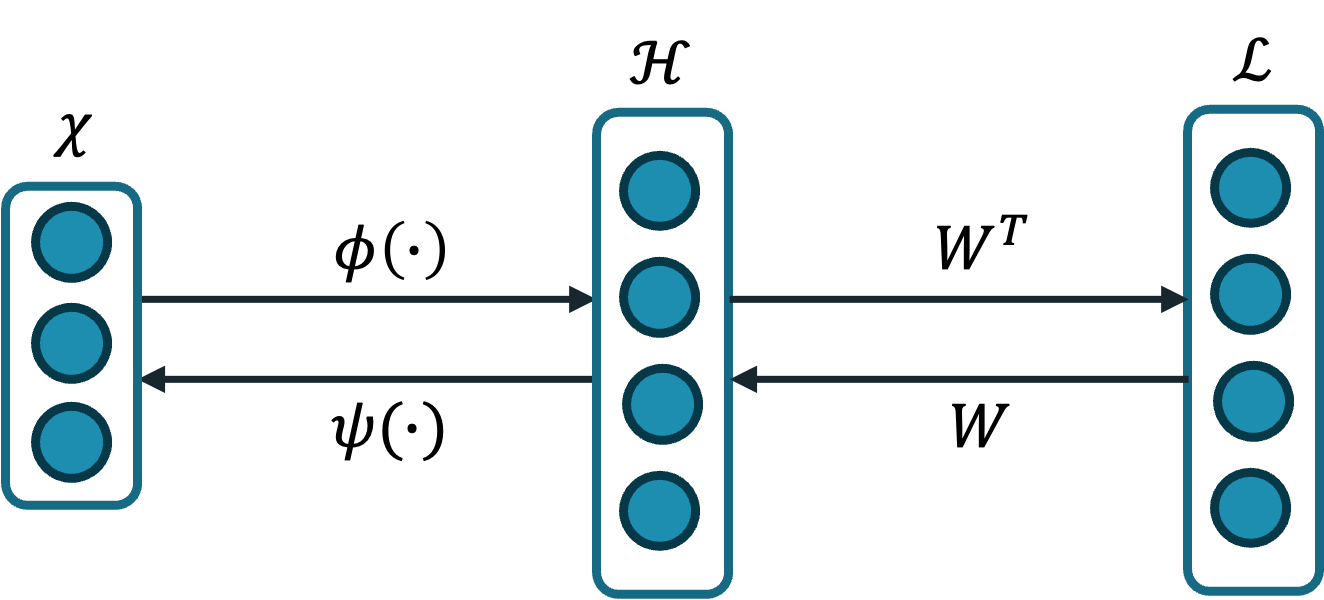
\includegraphics[width=0.7\linewidth]{Figures/PS/rkm_structure.png}
    \caption{Schematic representation of Gen-RKM. $\bphi(.)$ is the feature map network, while $\bpsi(.)$ corresponds to the pre-image network. $\bW$ is the interconnection matrix yielded from KPCA, mapping feature representations to the latent space $\mathcal{L}$. Latent points can be remapped back to the feature space via the transpose of the transformation matrix $\bW^{\top}$.}
    \label{rkm-demo}
\end{figure}

Next, a motivating example on the 012-MNIST dataset is used to illustrate the data imbalance issue in the Gen-RKM model. We consider an unbalanced version of the MNIST dataset, where only digits 0-2 are included and digit 2 is set to the minority class (see Section \ref{subsec-expr-datasets} for a more detailed introduction about the dataset used). Figure \ref{fig-latent-ub} (first row) shows the yielded latent space on the 012-MNIST dataset and the unbalanced version of it in the Gen-RKM setting. In the balanced dataset, well-separated or distinguishable clusters are produced in the latent space, and the corresponding latent representations are (nearly) evenly distributed, indicating each class has a similar influence on the learned latent space. As for the unbalanced scenario, it can be clearly observed that the learned latent space is strongly biased toward the majority groups since latent points from minority modes are mostly blurred or intermixed with the majority modes. The impact of data imbalance is significant on the latent space representation, where minority modes (or classes) are underrepresented, potentially leading to challenges in the generation or reconstruction of the underrepresented groups.

Data imbalance also has a similar effect on VAE as showcased in Figure \ref{fig-latent-ub} (second row), where the minority classes tend to be biased by the majority classes. That is unsurprising, as Gen-RKM and VAE share similar encoder-decoder architectures, and the data distribution in both models is explicitly defined. The biases in the final generation results brought by data imbalance are confirmed in Figure \ref{fig-mnist}, where random generations from both balanced and unbalanced datasets are depicted. One can observe that samples from minority classes are generated much less frequently than those from majority classes.

To extend the capability of Gen-RKM to generalize well to the minority classes in the unbalanced data, a natural idea is to augment the minority classes in the latent space (in other words, synthetically increasing the number of latent points corresponding to minority modes). In this spirit, the generation result should be more diverse. Of course, this approach is equivalent to performing augmentation on the original data, as only a balanced distribution of raw data can result in a balanced distribution in its corresponding latent space. In the next chapter, we will discuss random sampling, a naive yet effective approach for addressing data imbalance. Specifically, we will combine various sampling techniques with Gen-RKM  framework to investigate how to tackle the issue of unbalanced data in the generative learning context.

% Figure \ref{fig-latent-ub} shows the latent space of the MNIST012 datasets and the unbalanced version of it. When the dataset is unbalanced (The number of digit 2 is only 10\% of the numbers of 0 and 1), it is hard to observe the representation of the minority class in the latent space. And GMM estimation tends to treat these minorities as noise, resulting in a low probability of sampling from these groups when generating new samples. Figure \ref{fig-mnist} compares the randomly generated samples from the latent spaces in Figure \ref{fig-latent-ub} respectively. There are almost no samples from minority classes generated from the unbalanced latent space. 




\begin{figure}[H]
    \centering
    \begin{subfigure}{0.45\textwidth}
        \centering
        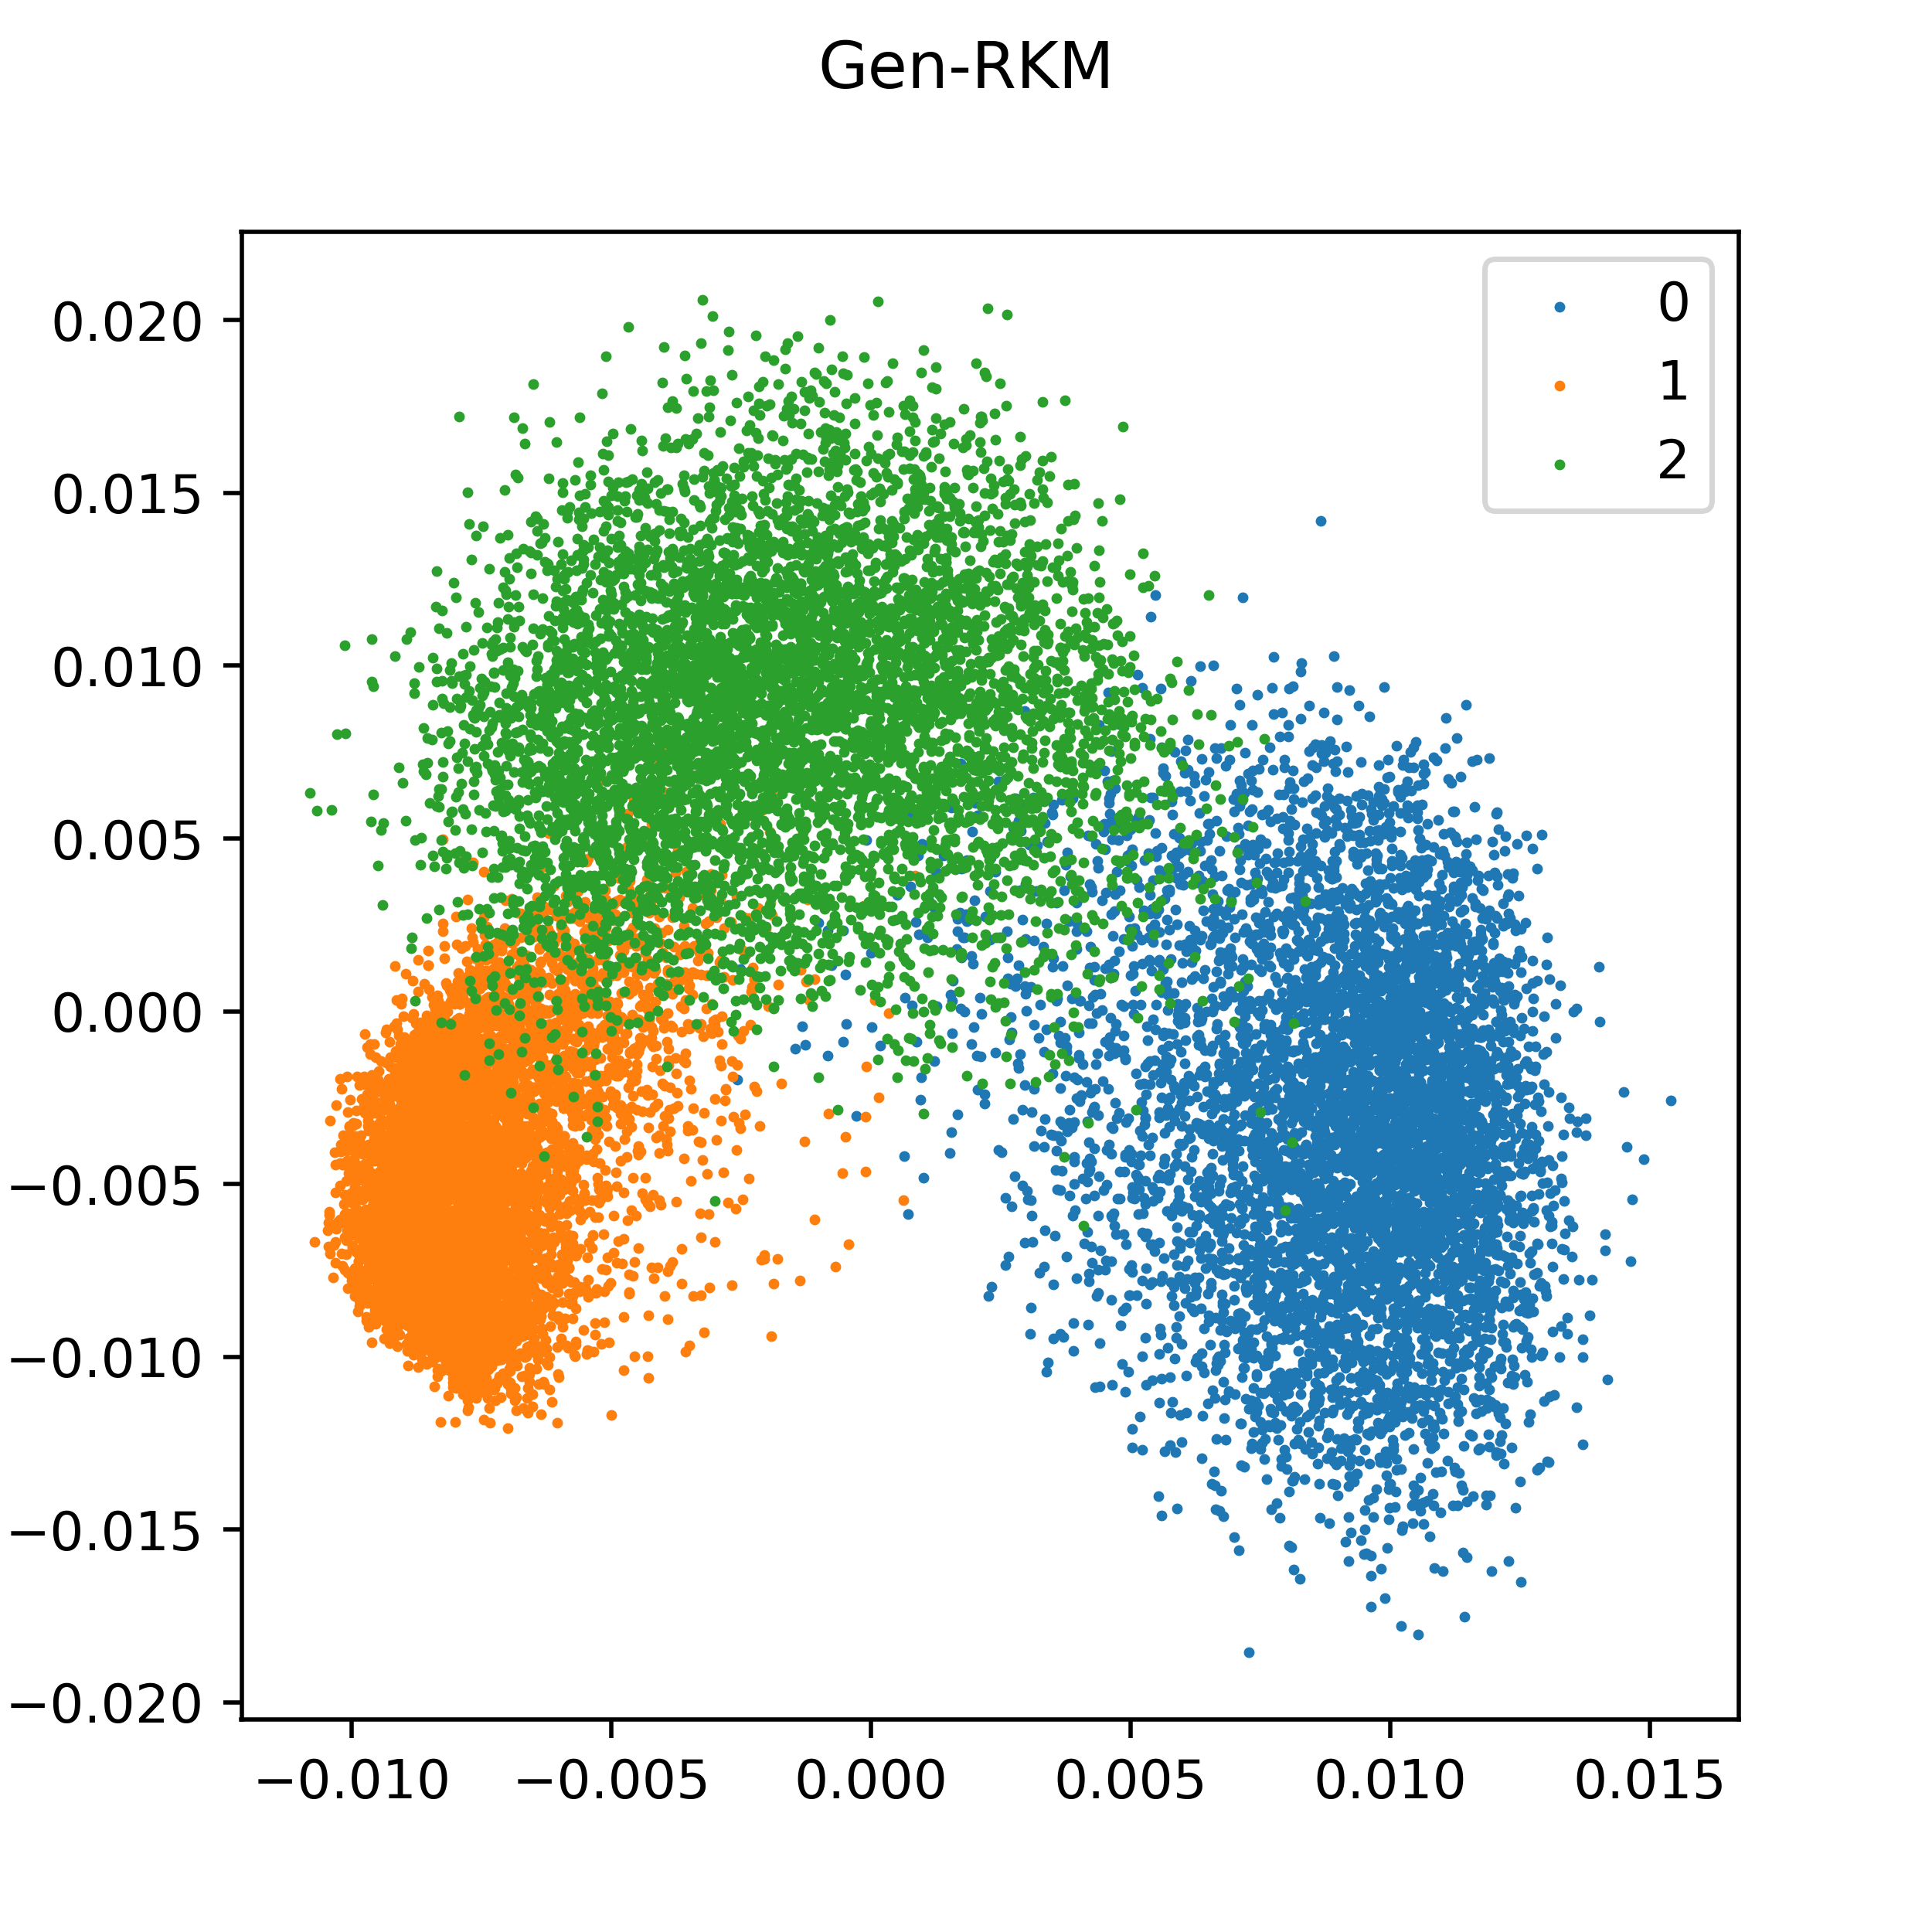
\includegraphics[width=0.8\textwidth]{Figures/PS_v2/rkm-bMNIST012-latentspace-vis.png}
    \end{subfigure}
    \hfill
    \begin{subfigure}{0.45\textwidth}
        \centering
        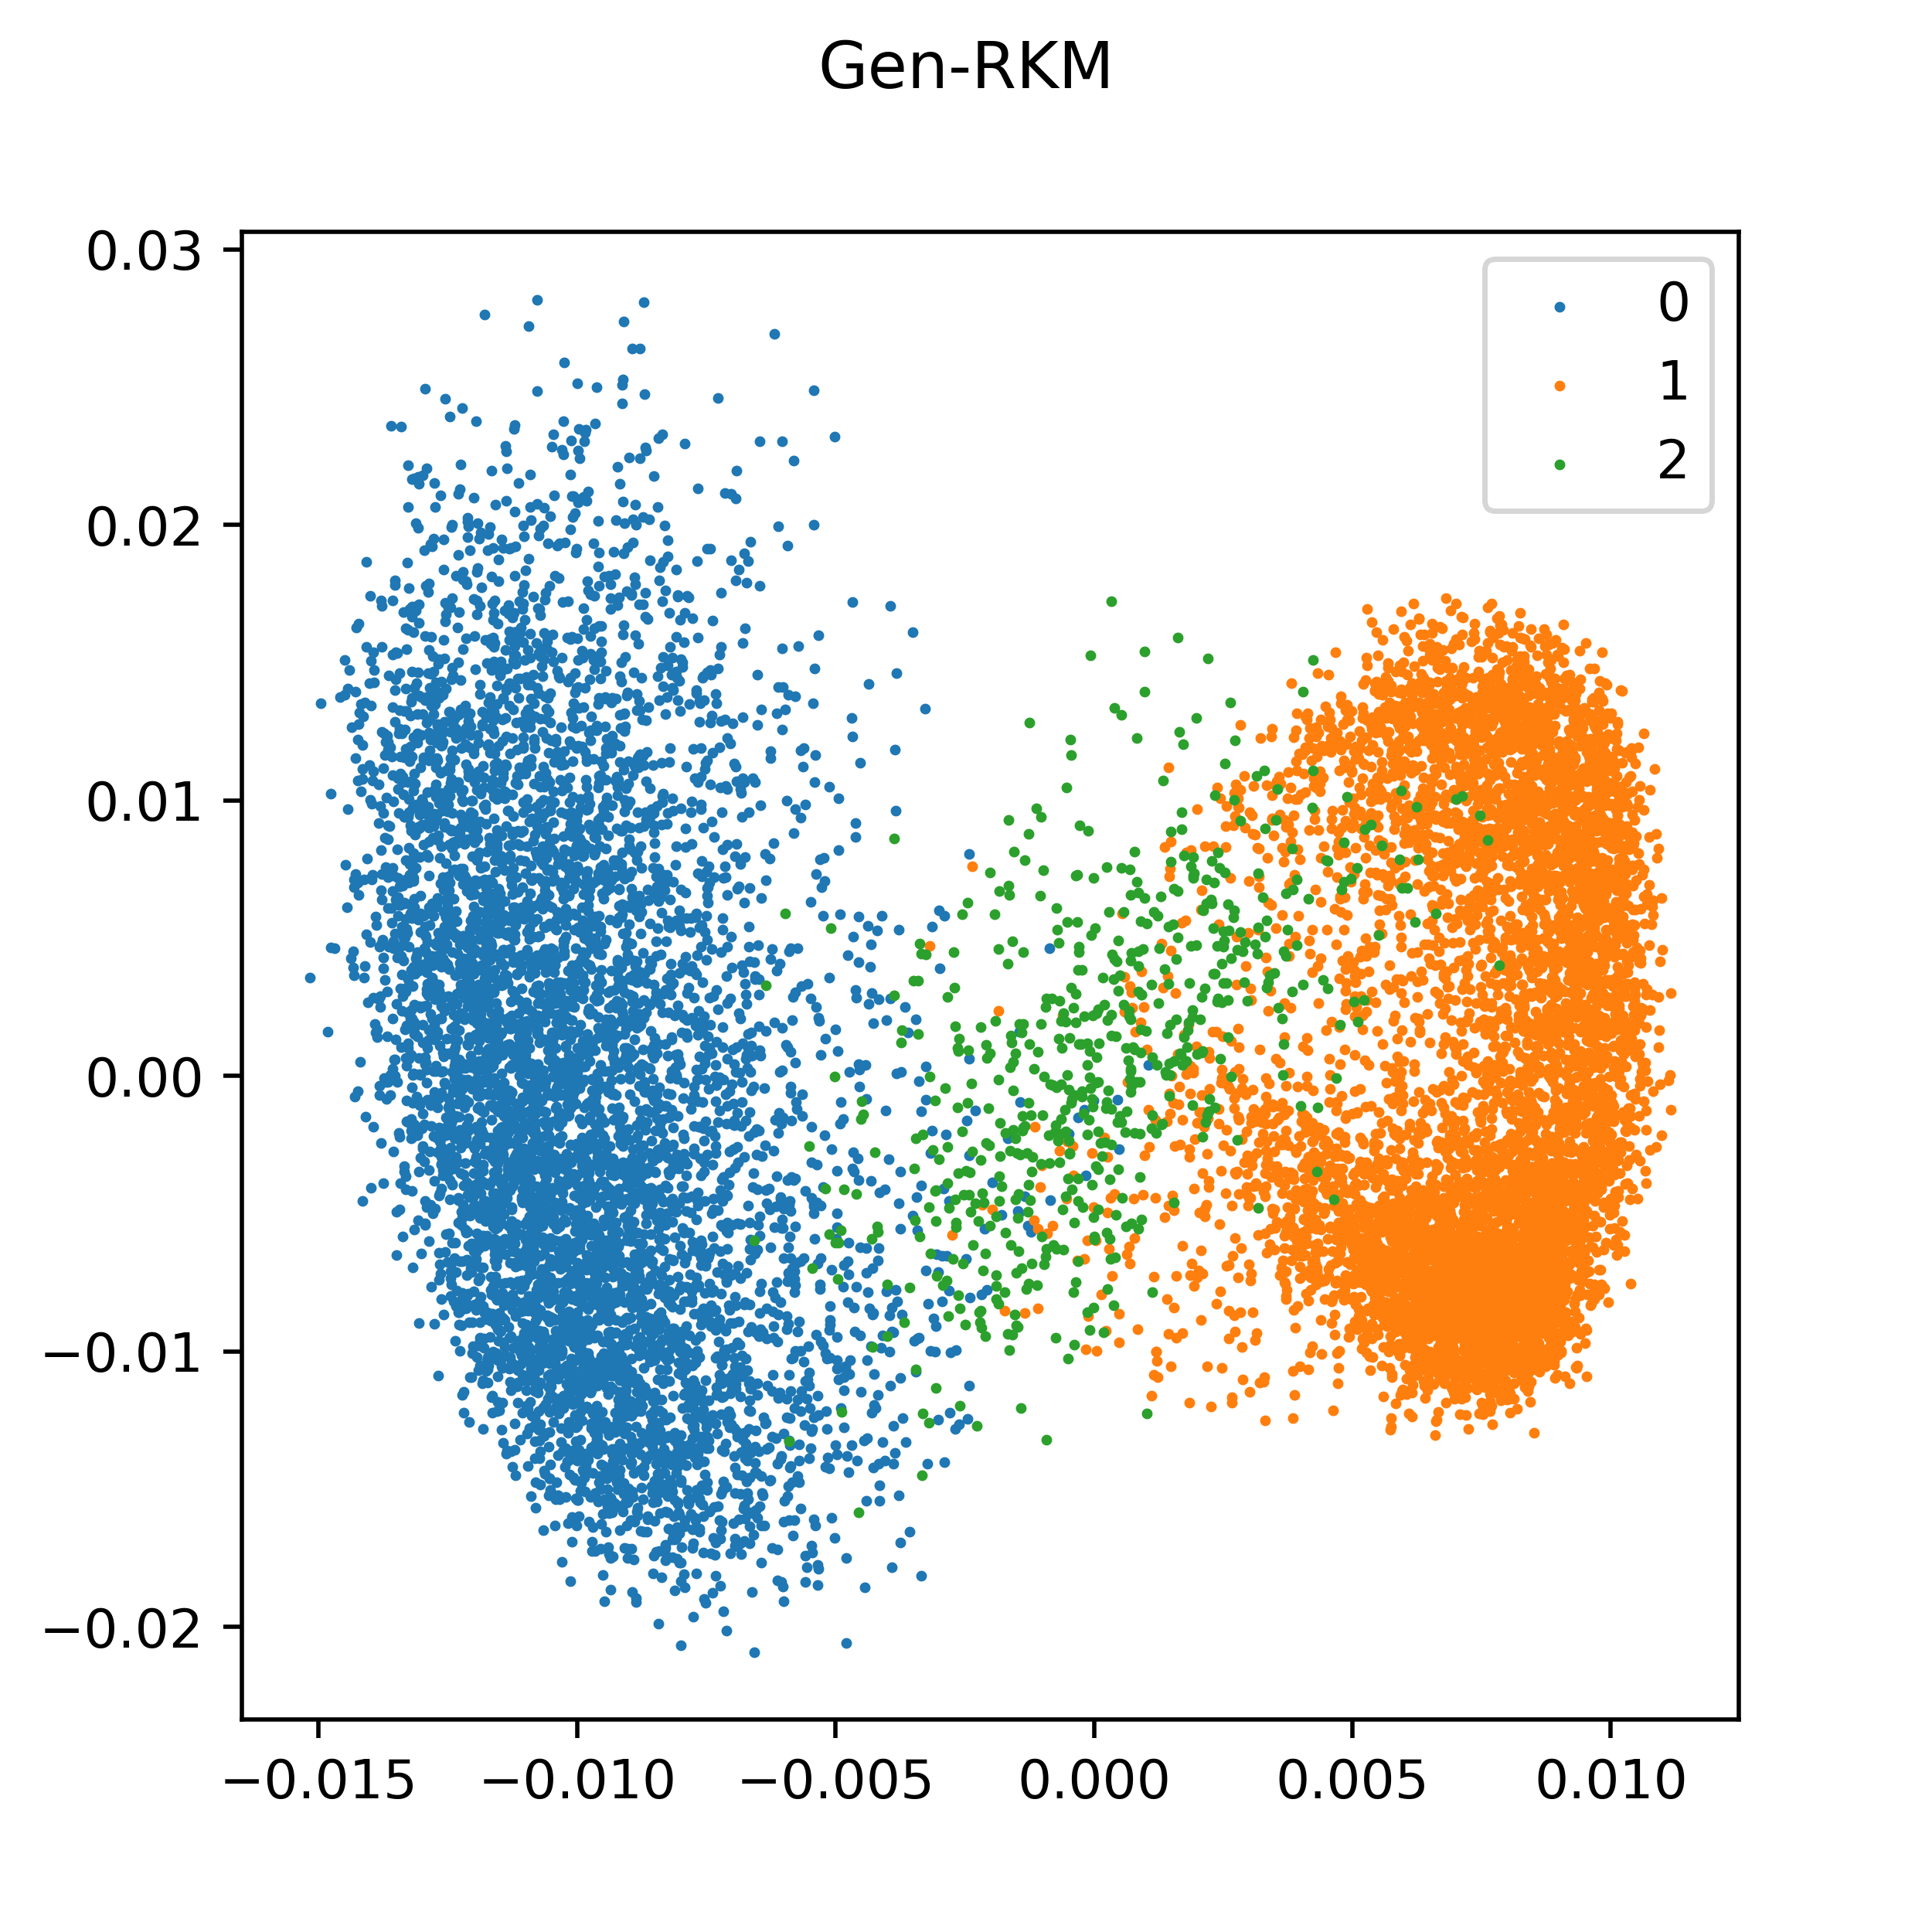
\includegraphics[width=0.8\textwidth]{Figures/PS_v2/rkm-ubMNIST012-latentspace-vis.png}
    \end{subfigure}
    \vfill
    \begin{subfigure}{0.45\textwidth}
        \centering
        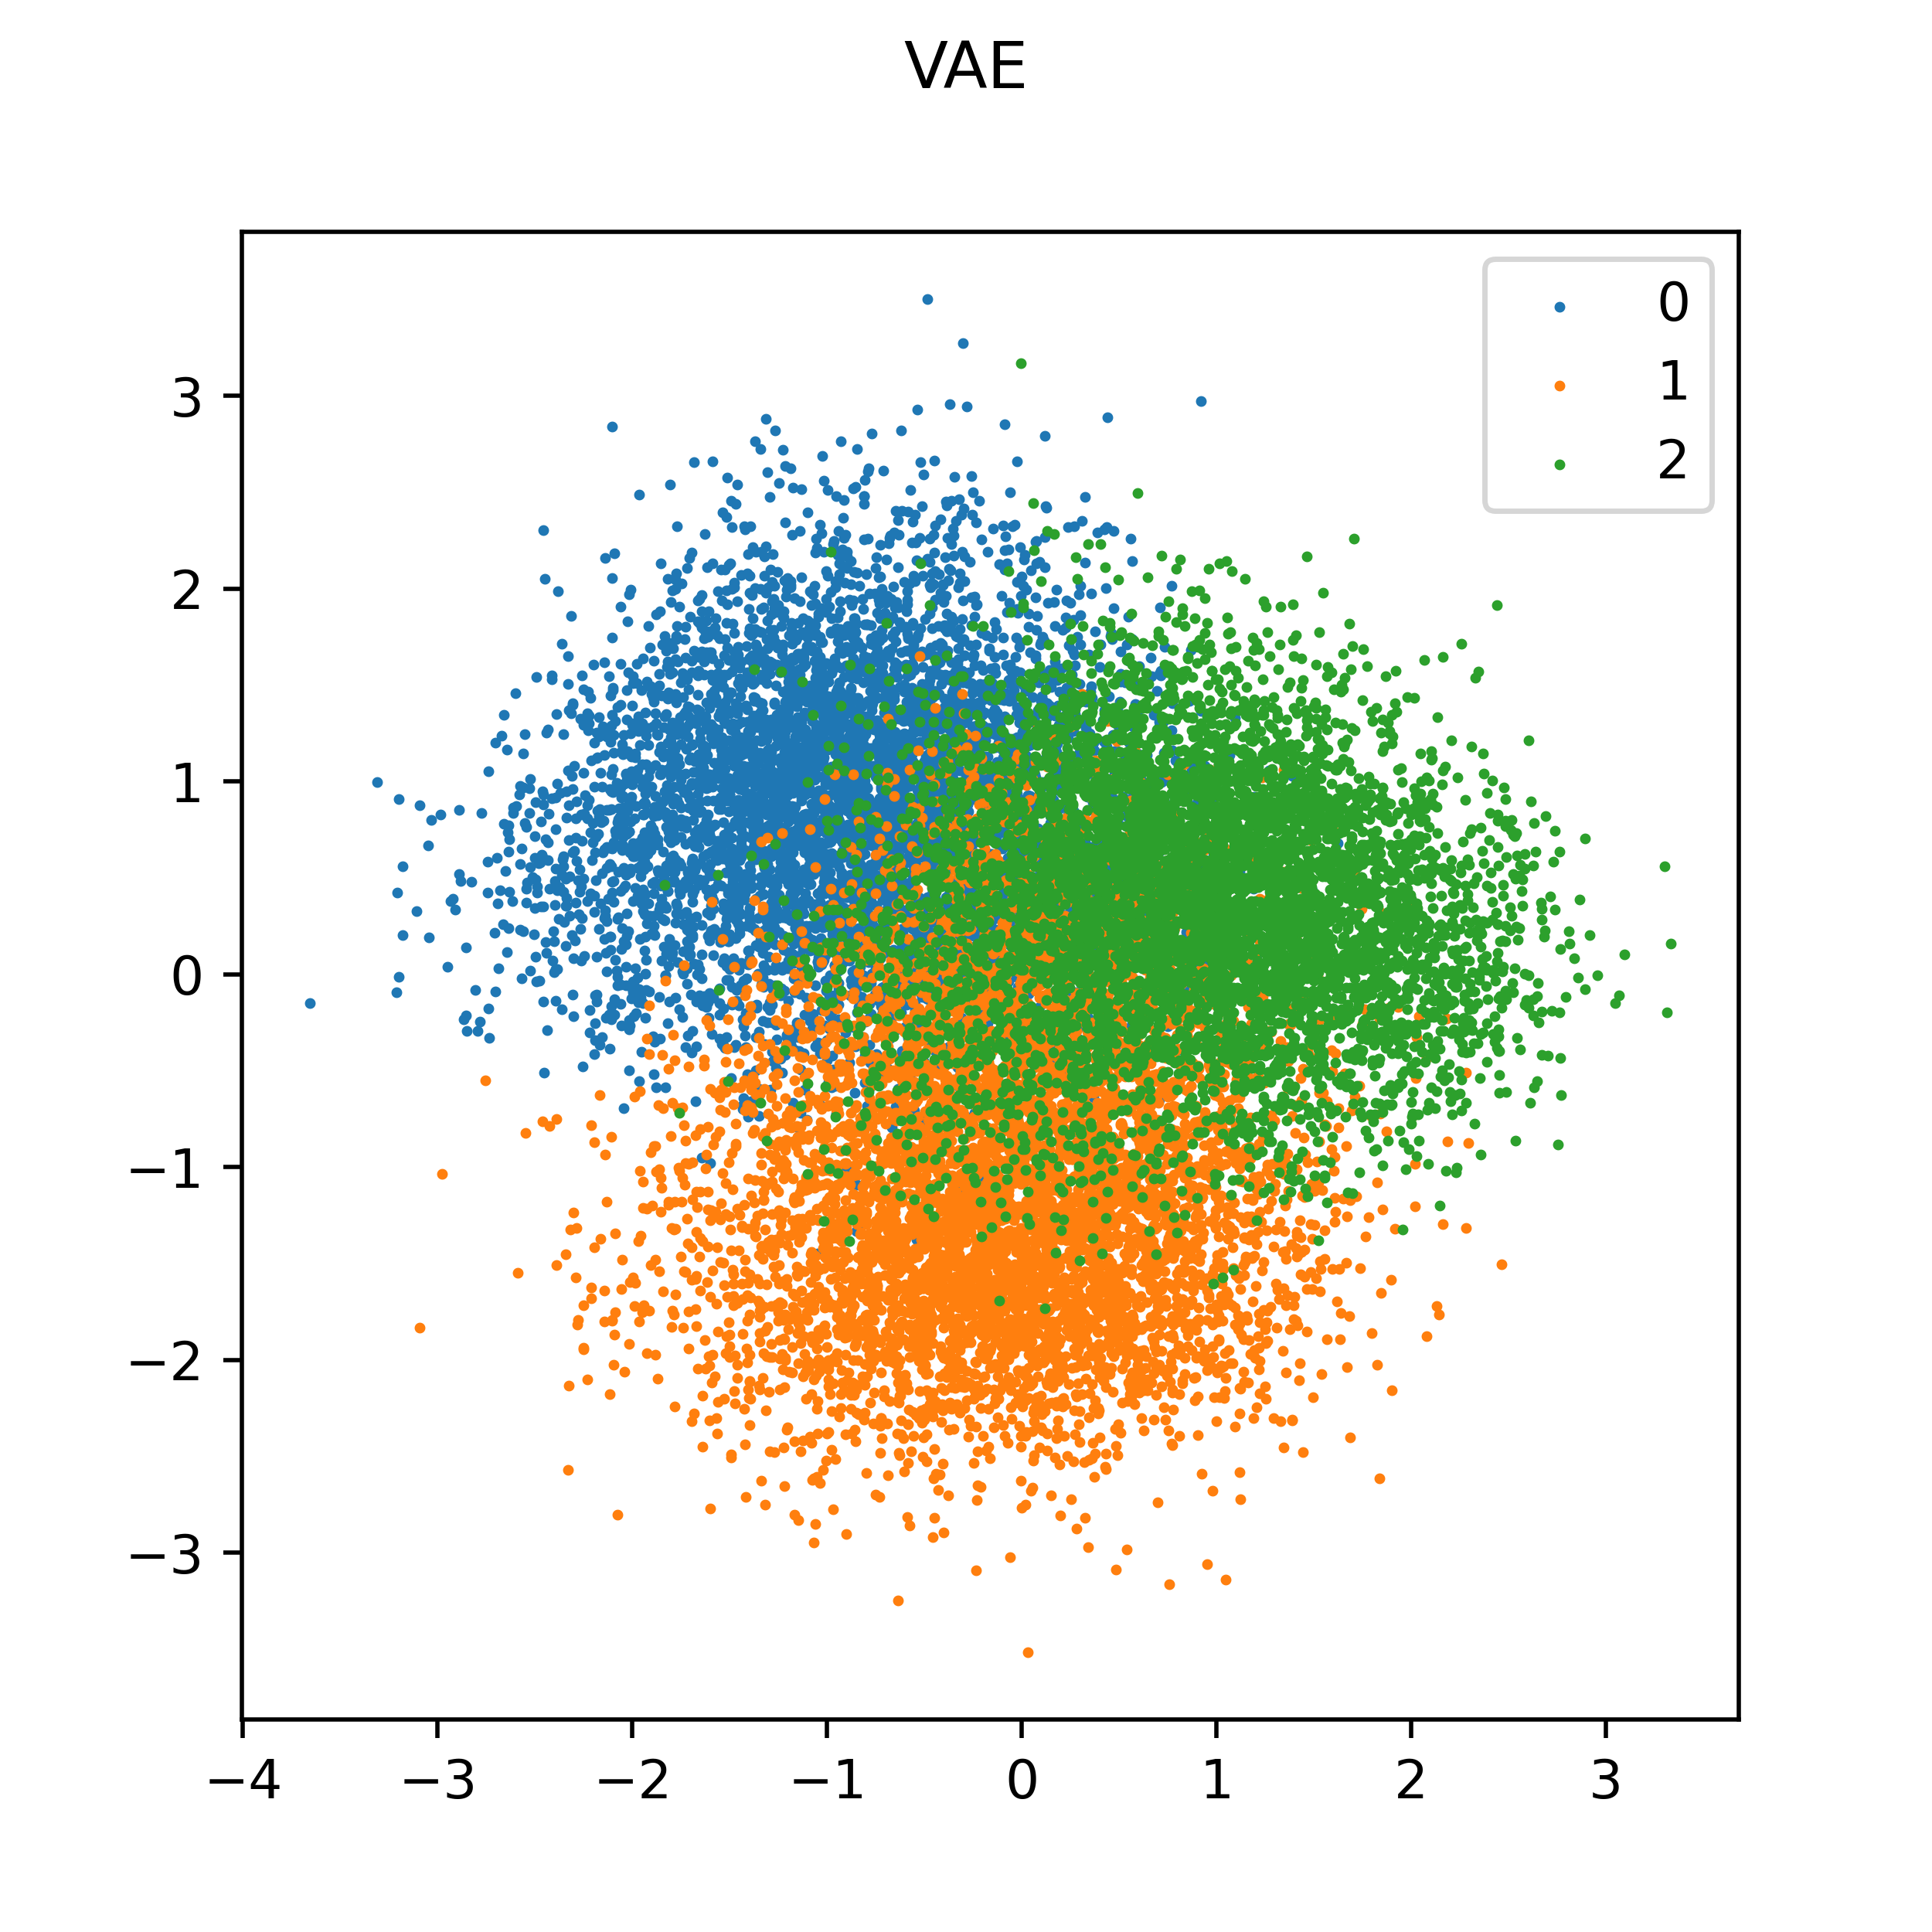
\includegraphics[width=0.8\textwidth]{Figures/PS_v2/vae-bMNIST012-latentspace-vis.png} % Replace with your third image path
    \end{subfigure}
    \hfill
    \begin{subfigure}{0.45\textwidth}
        \centering
        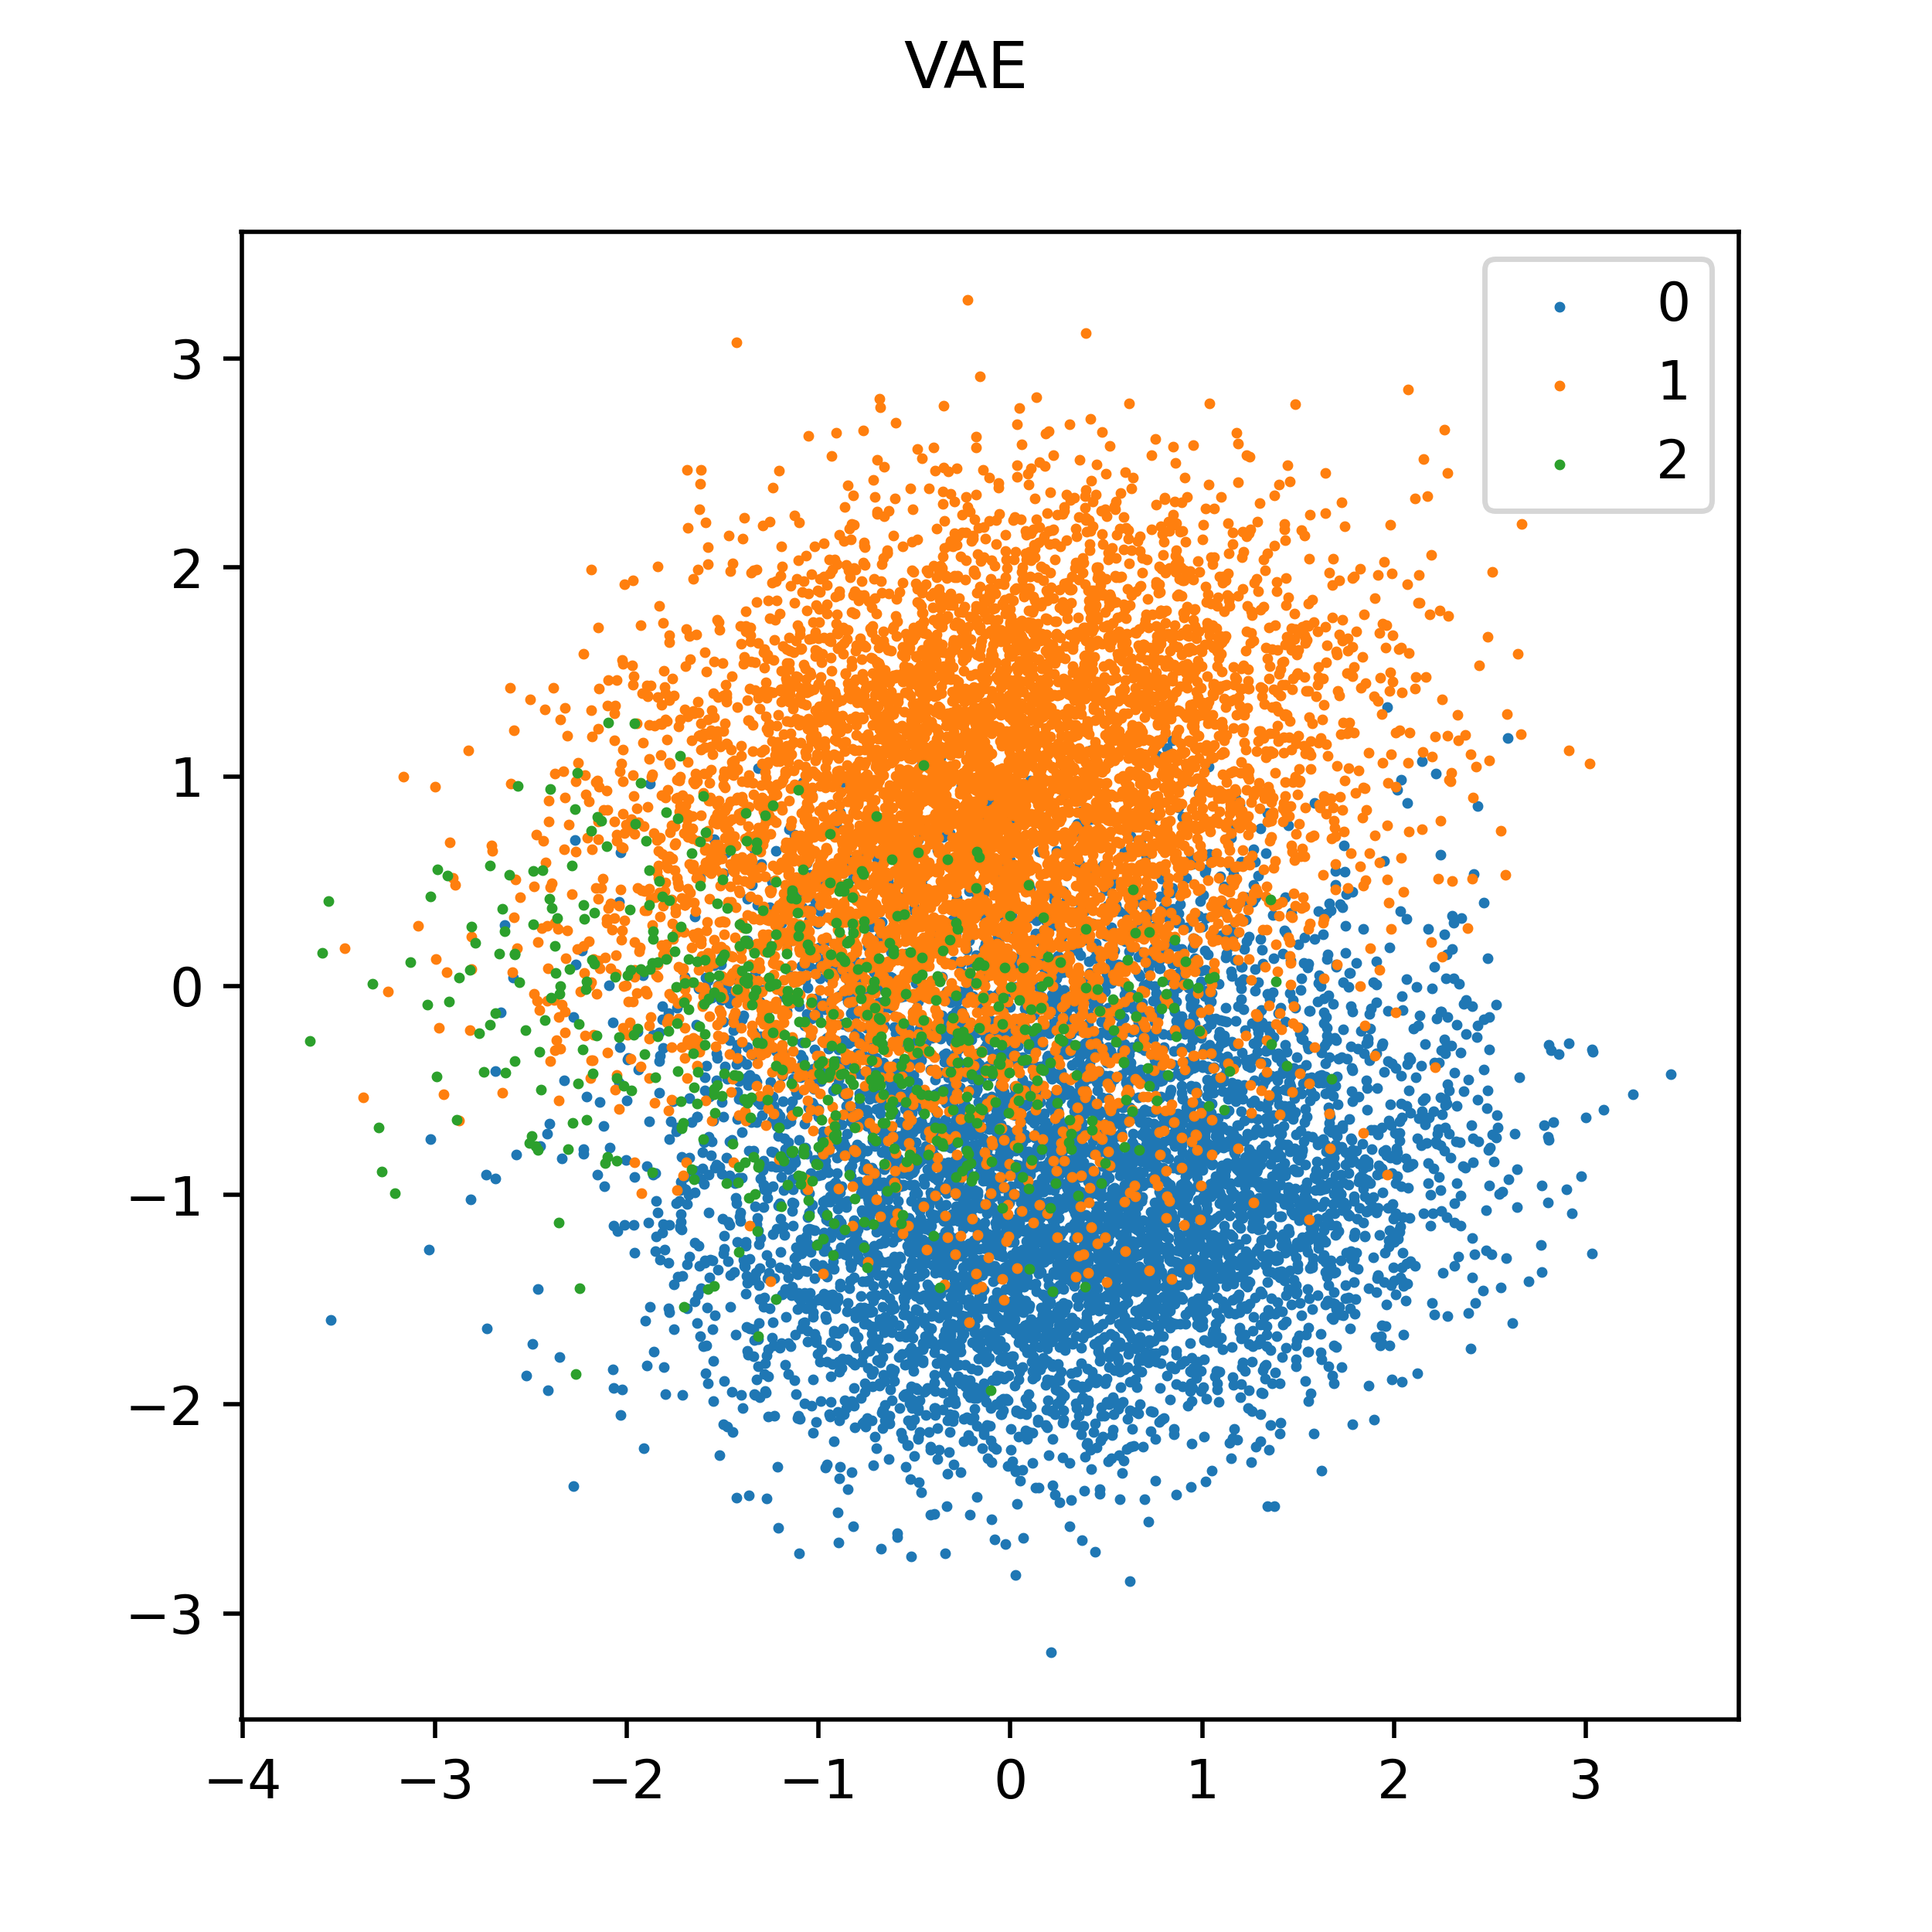
\includegraphics[width=0.8\textwidth]{Figures/PS_v2/vae-ubMNIST012-latentspace-vis.png} % Replace with your fourth image path
    \end{subfigure}
    \caption{Visualizations of latent spaces of Gen-RKM (first row) and VAE (second row) trained on balanced (first column) and unbalanced 012-MNIST datasets (second columns). The minority mode is depicted in green color. Sizes of latent space of both Gen-RKM and VAE are set to 10, and only the first two dimensions are visualized.}
    \label{fig-latent-ub}
\end{figure}


% \begin{figure}[H]
%     \centering
%     \begin{subfigure}{0.45\textwidth}
%         \centering
%         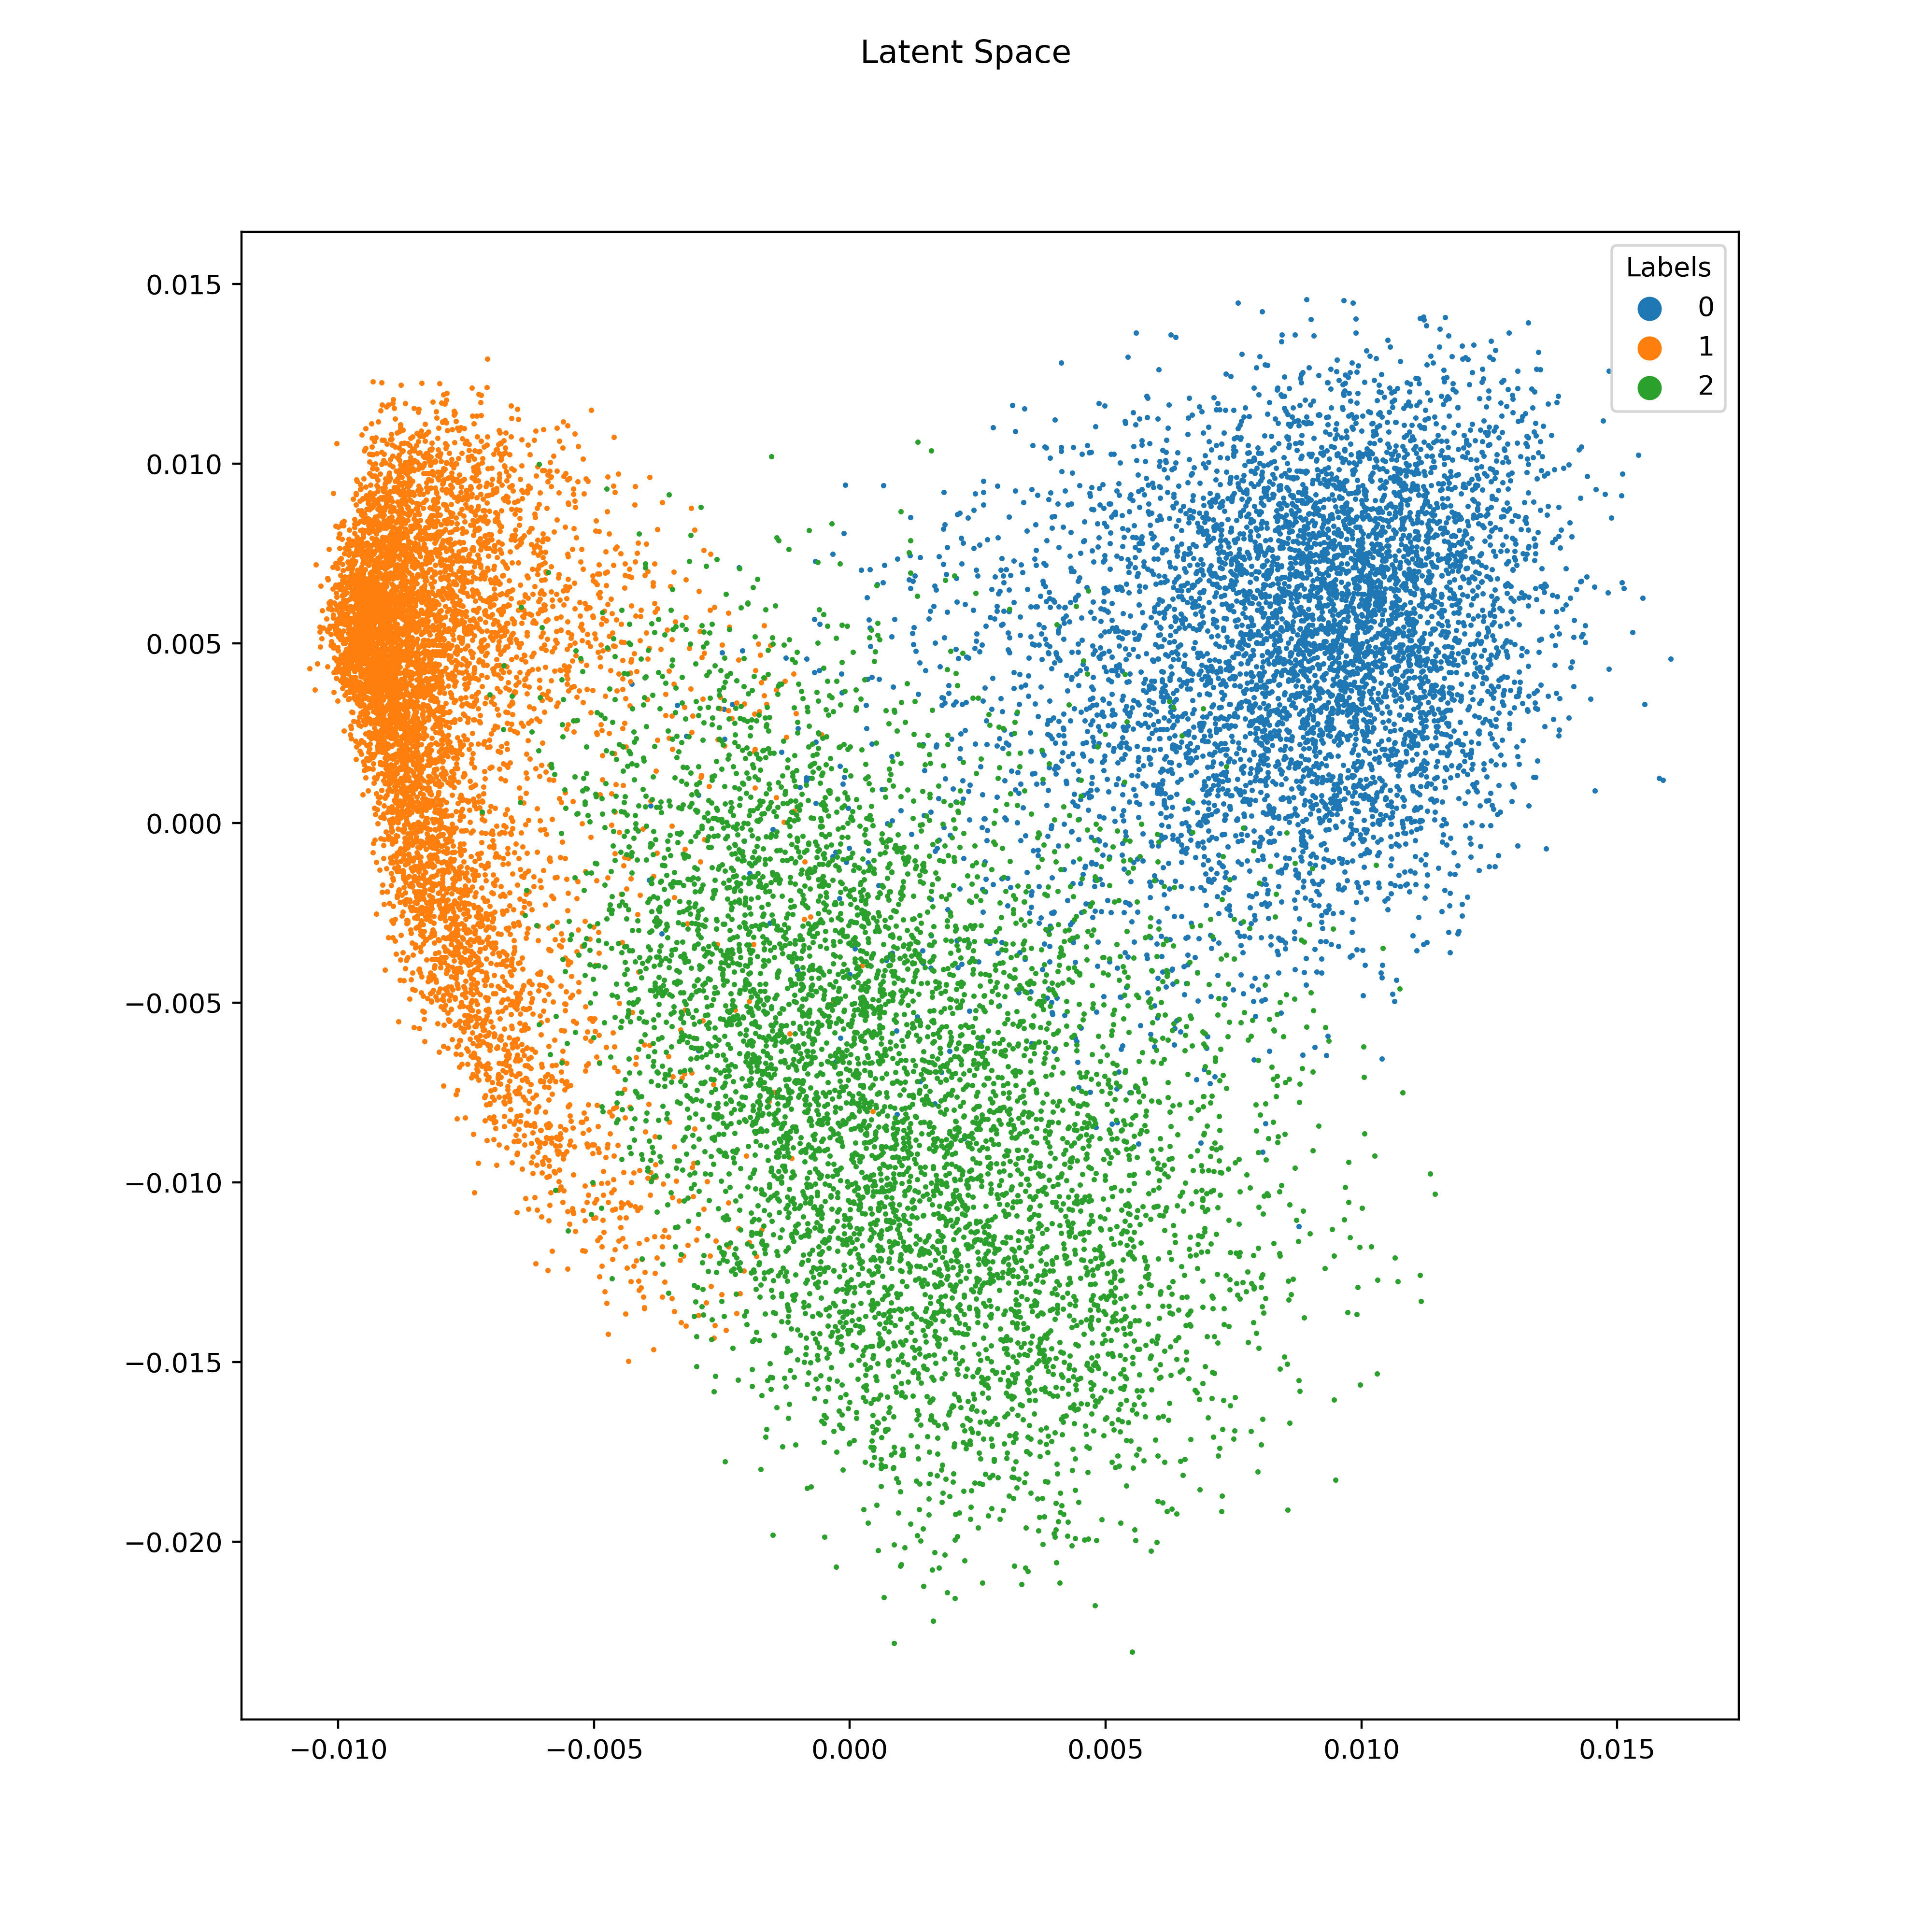
\includegraphics[width=0.8\textwidth]{Figures/PS/b012_latent_space.png}
%     \end{subfigure}
%     \hfill
%     \begin{subfigure}{0.45\textwidth}
%         \centering
%         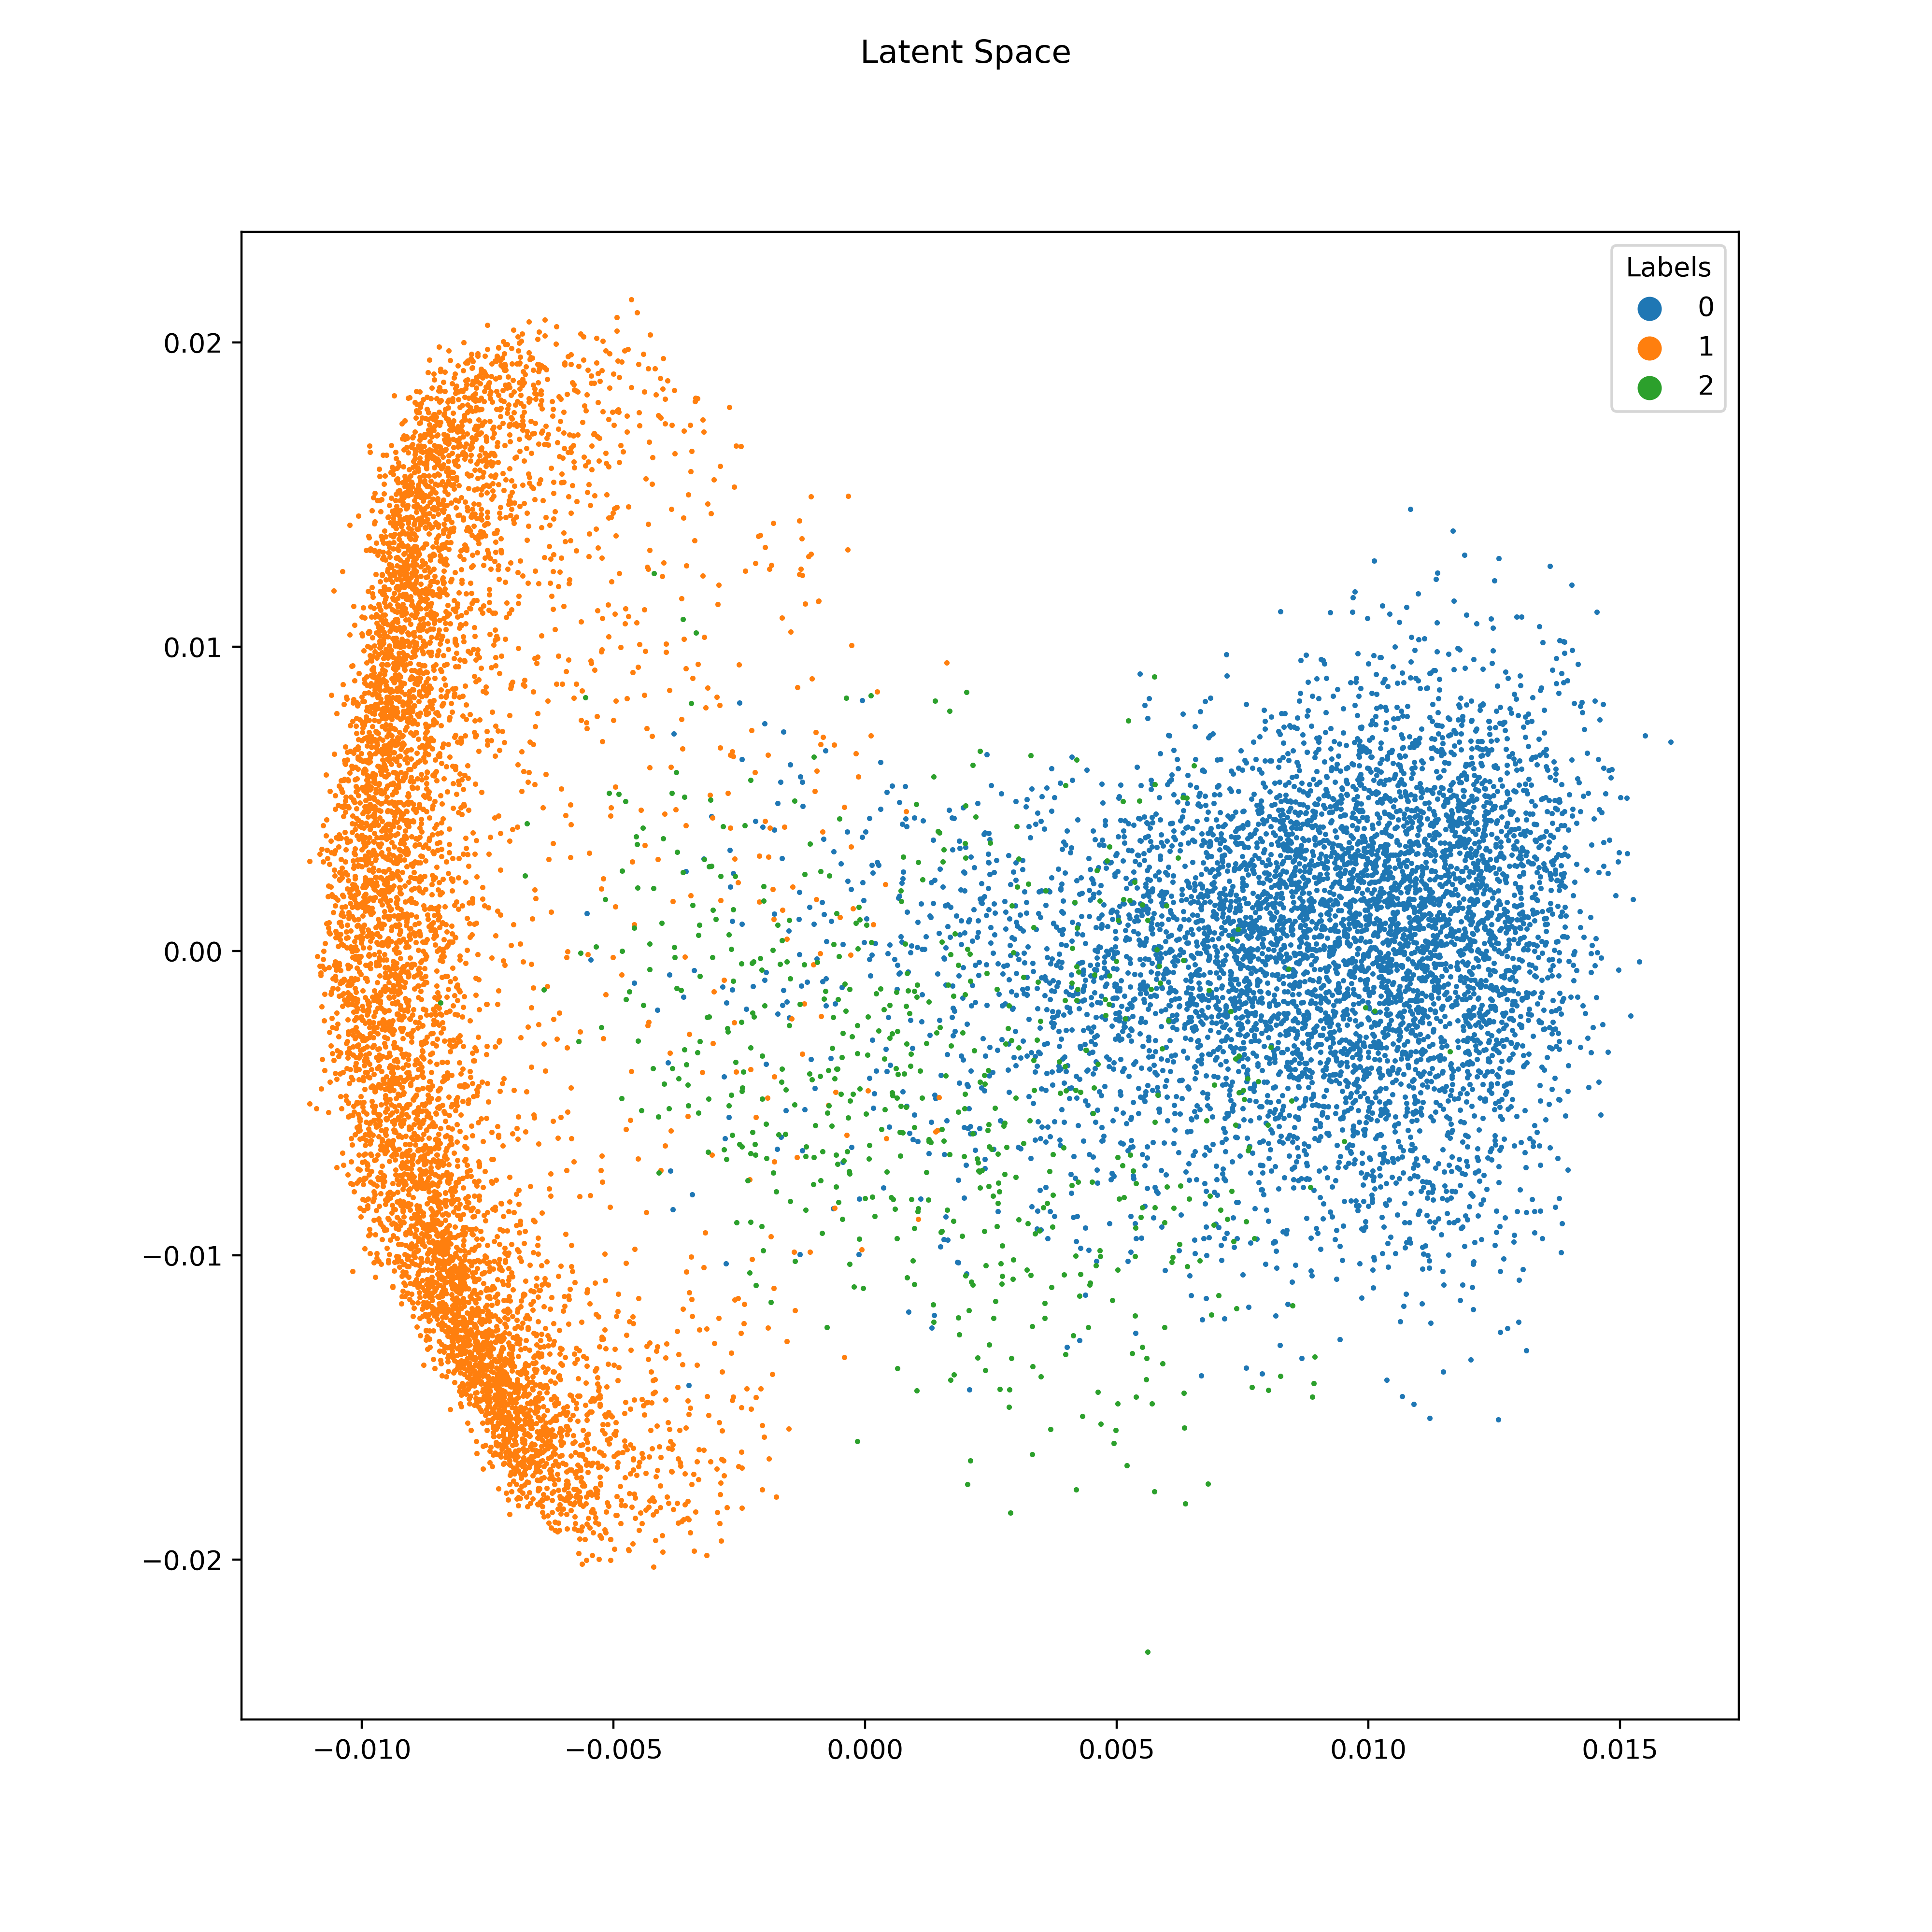
\includegraphics[width=0.8\textwidth]{Figures/PS/ub012_latent_space.png}
%     \end{subfigure}
%     \caption{Latent space of 012-MNIST: balanced (left) and unbalanced(right)}
%     \label{fig-latent-ub}
% \end{figure}

% \begin{figure}[H]
%     \centering
%     \begin{subfigure}{0.45\textwidth}
%         \centering
%         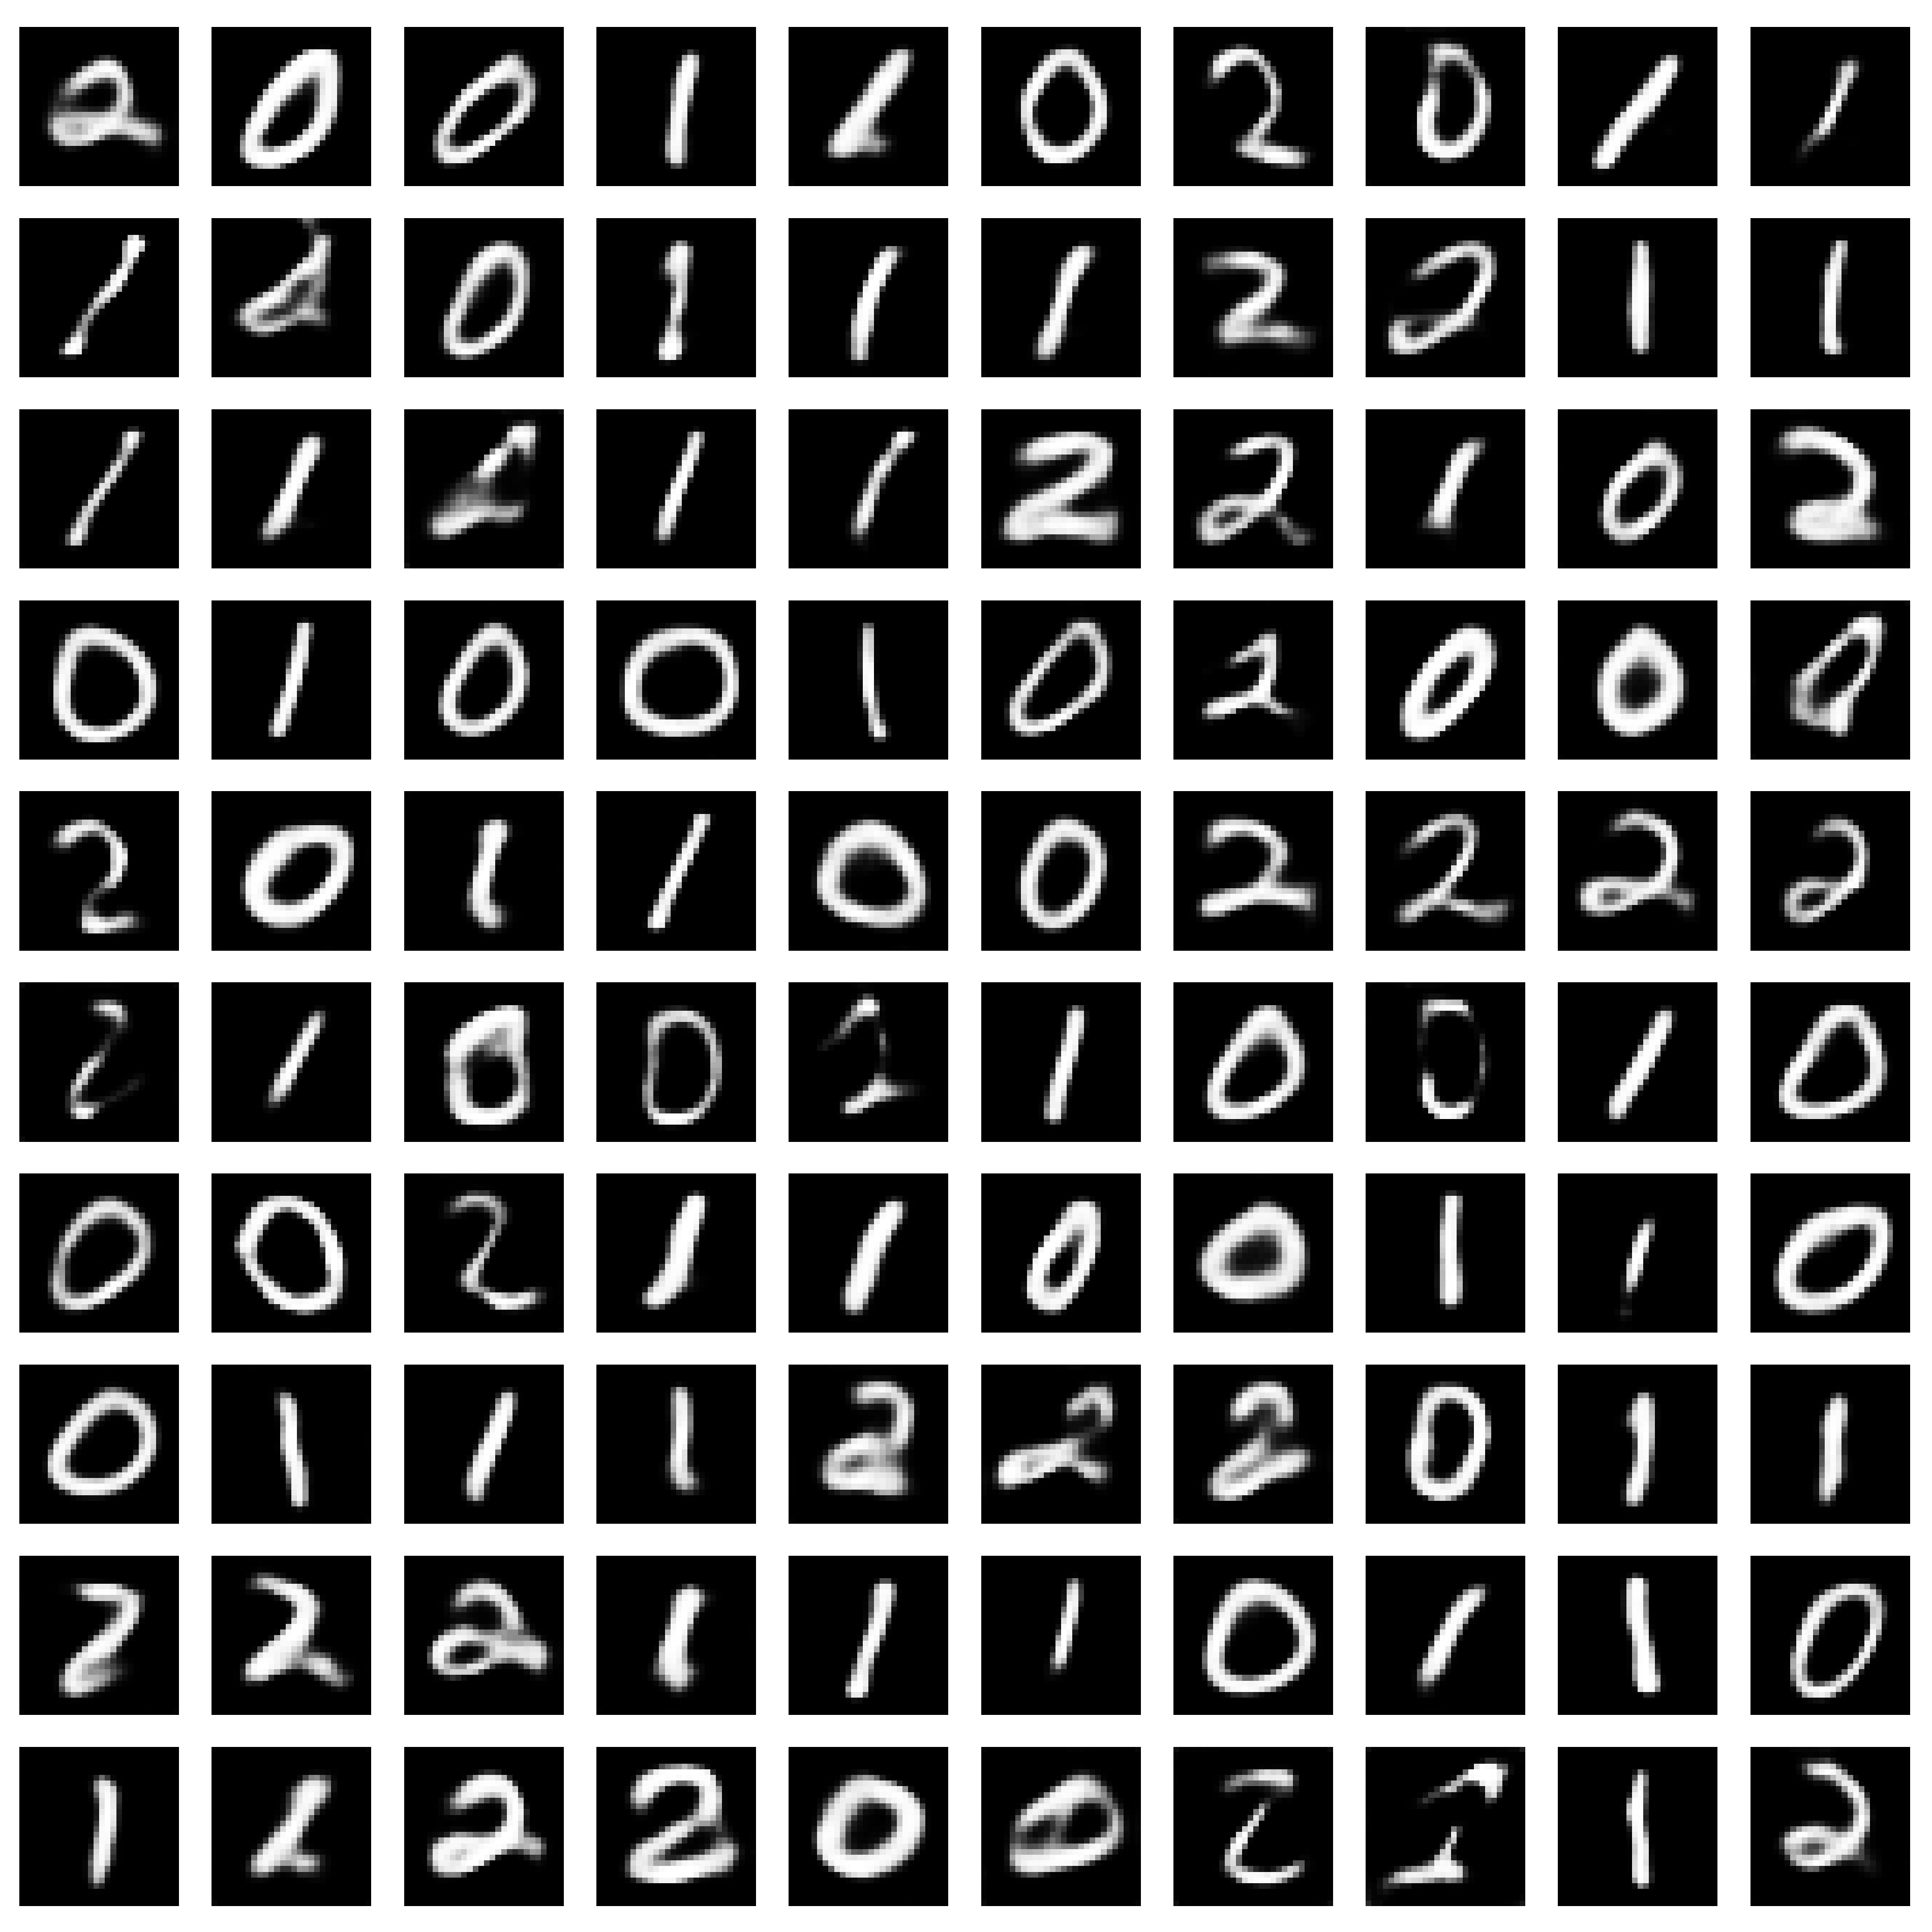
\includegraphics[width=0.8\textwidth]{Figures/PS/b012_random_generation.png}
%     \end{subfigure}
%     \hfill
%     \begin{subfigure}{0.45\textwidth}
%         \centering
%         
\includegraphics[width=0.8\textwidth]{Figures/PS/ub012_random_generation.png}
%     \end{subfigure}
%     \caption{Random generation of MNIST012: balanced (left) and unbalanced(right)}
%     \label{fig-mnist}
% \end{figure}

\begin{figure}[htb]
    \centering
    \begin{subfigure}{0.24\textwidth}
        \centering
        
\includegraphics[width=0.9\textwidth]{Figures/PS_v2/genrkm-bMNIST012-gensamples.png}
    \end{subfigure}
    \hfill
    \begin{subfigure}{0.24\textwidth}
        \centering
        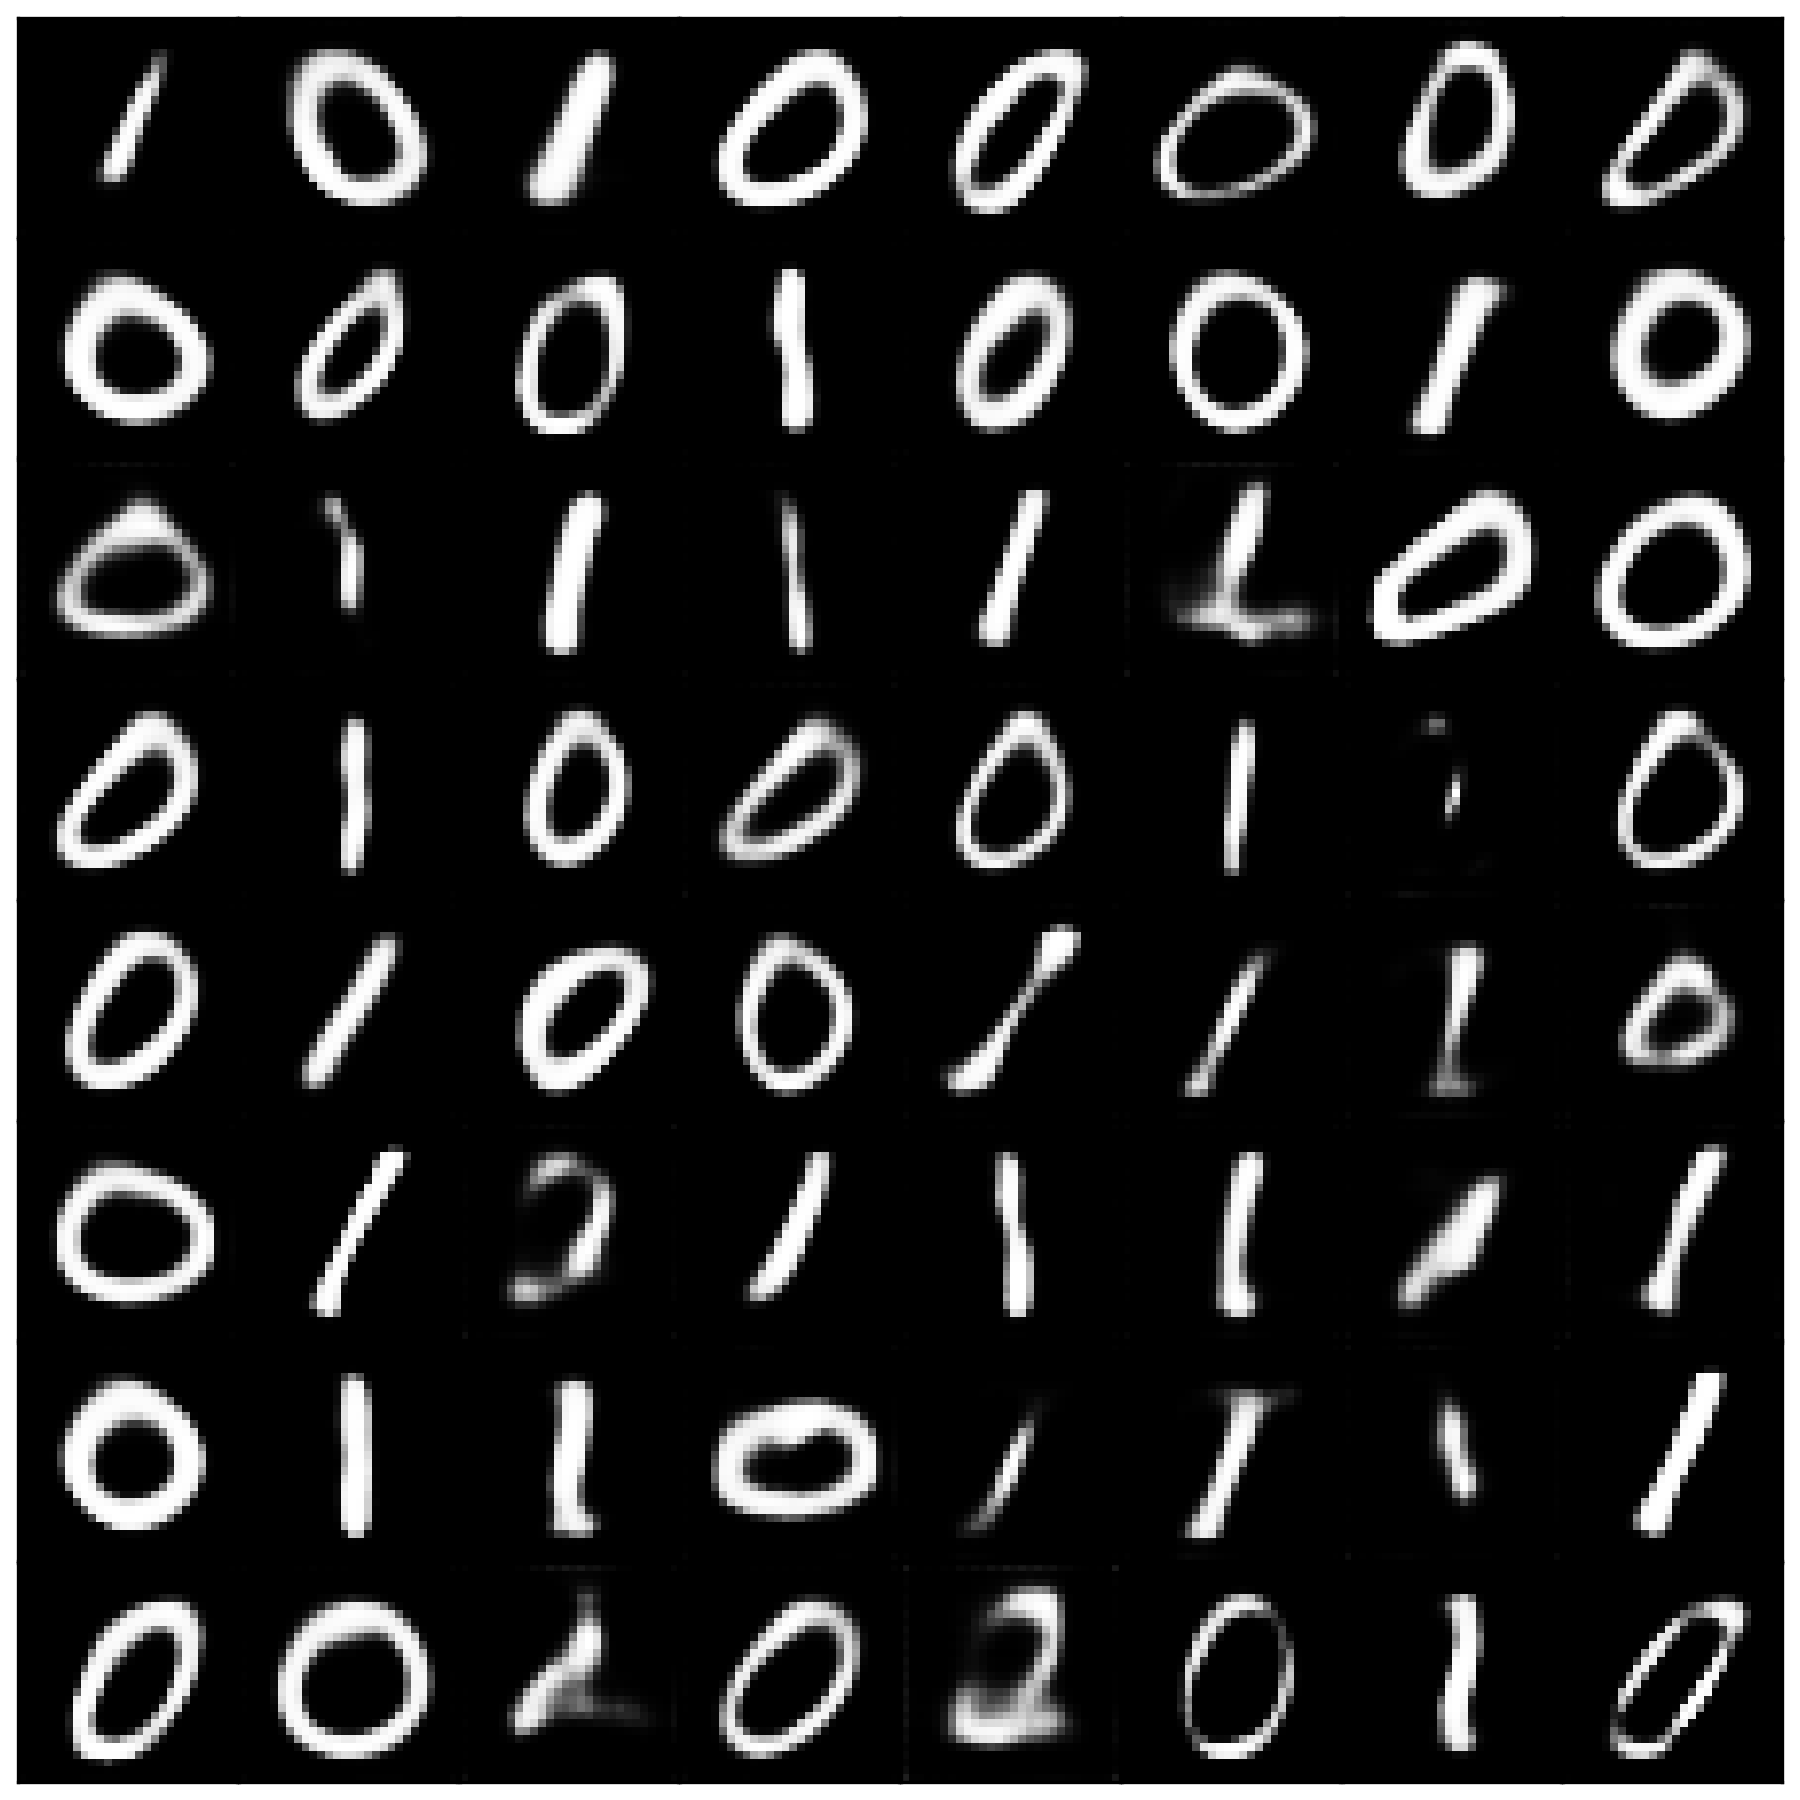
\includegraphics[width=0.9\textwidth]{Figures/PS_v2/genrkm-ubMNIST012-gensamples.png}
    \end{subfigure}
    \hfill
    \begin{subfigure}{0.24\textwidth}
        \centering
        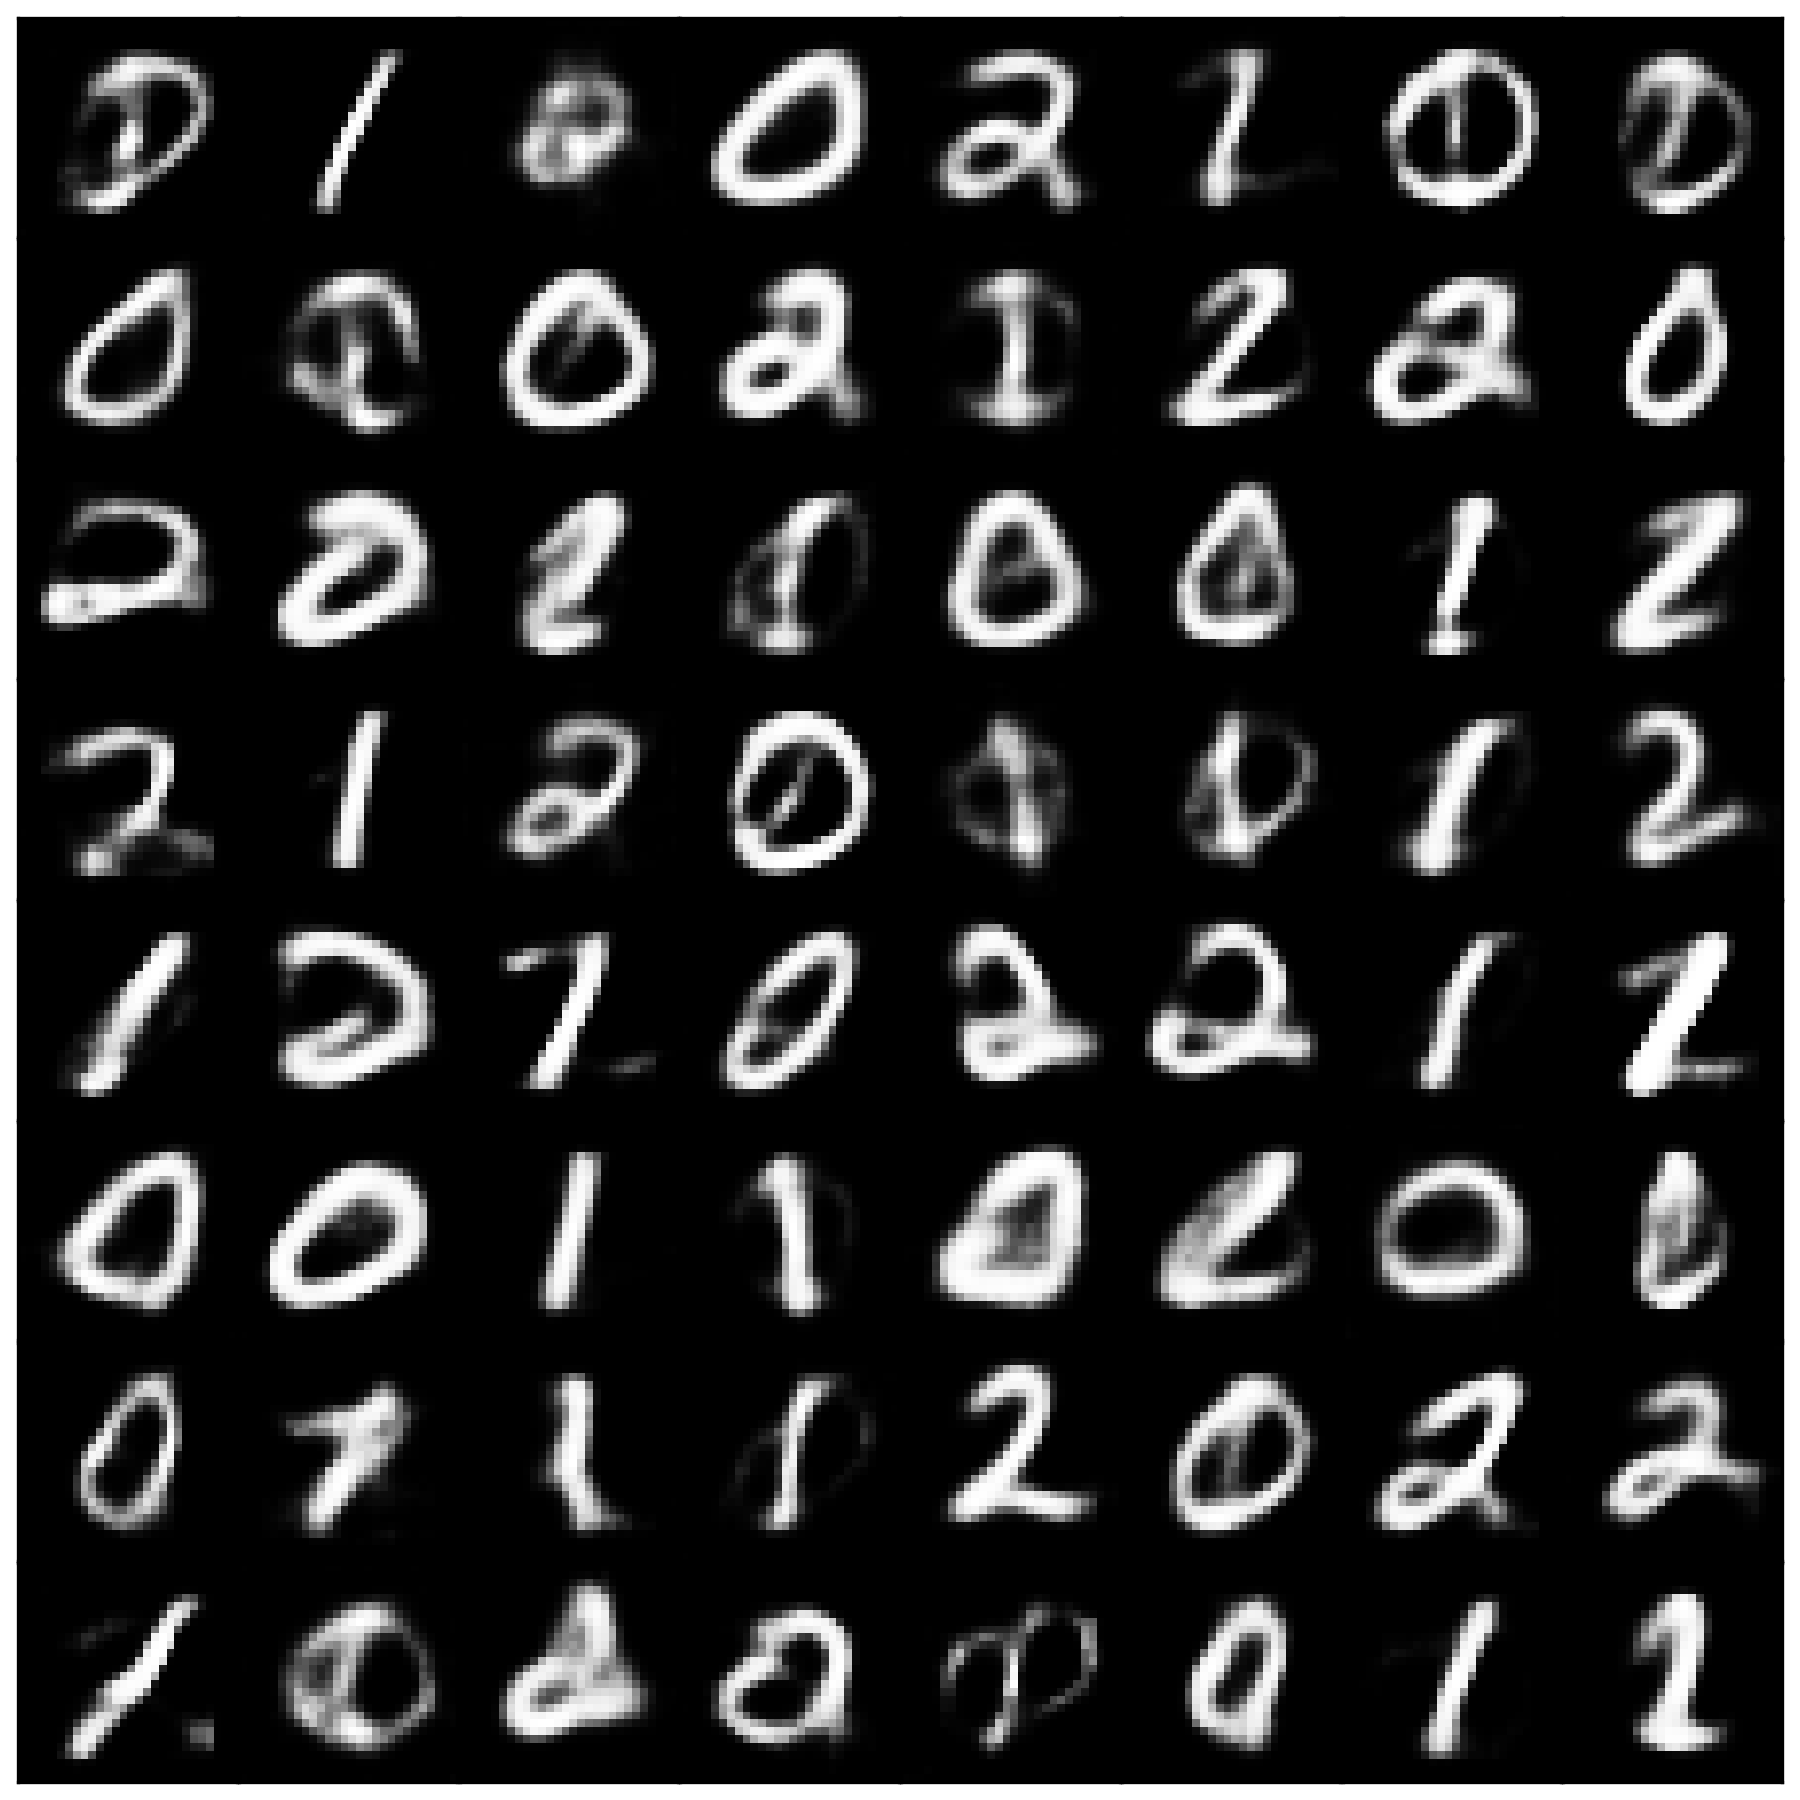
\includegraphics[width=0.9\textwidth]{Figures/PS_v2/vae-bMNIST012-gensamples.png}
    \end{subfigure}
    \hfill
    \begin{subfigure}{0.24\textwidth}
        \centering
        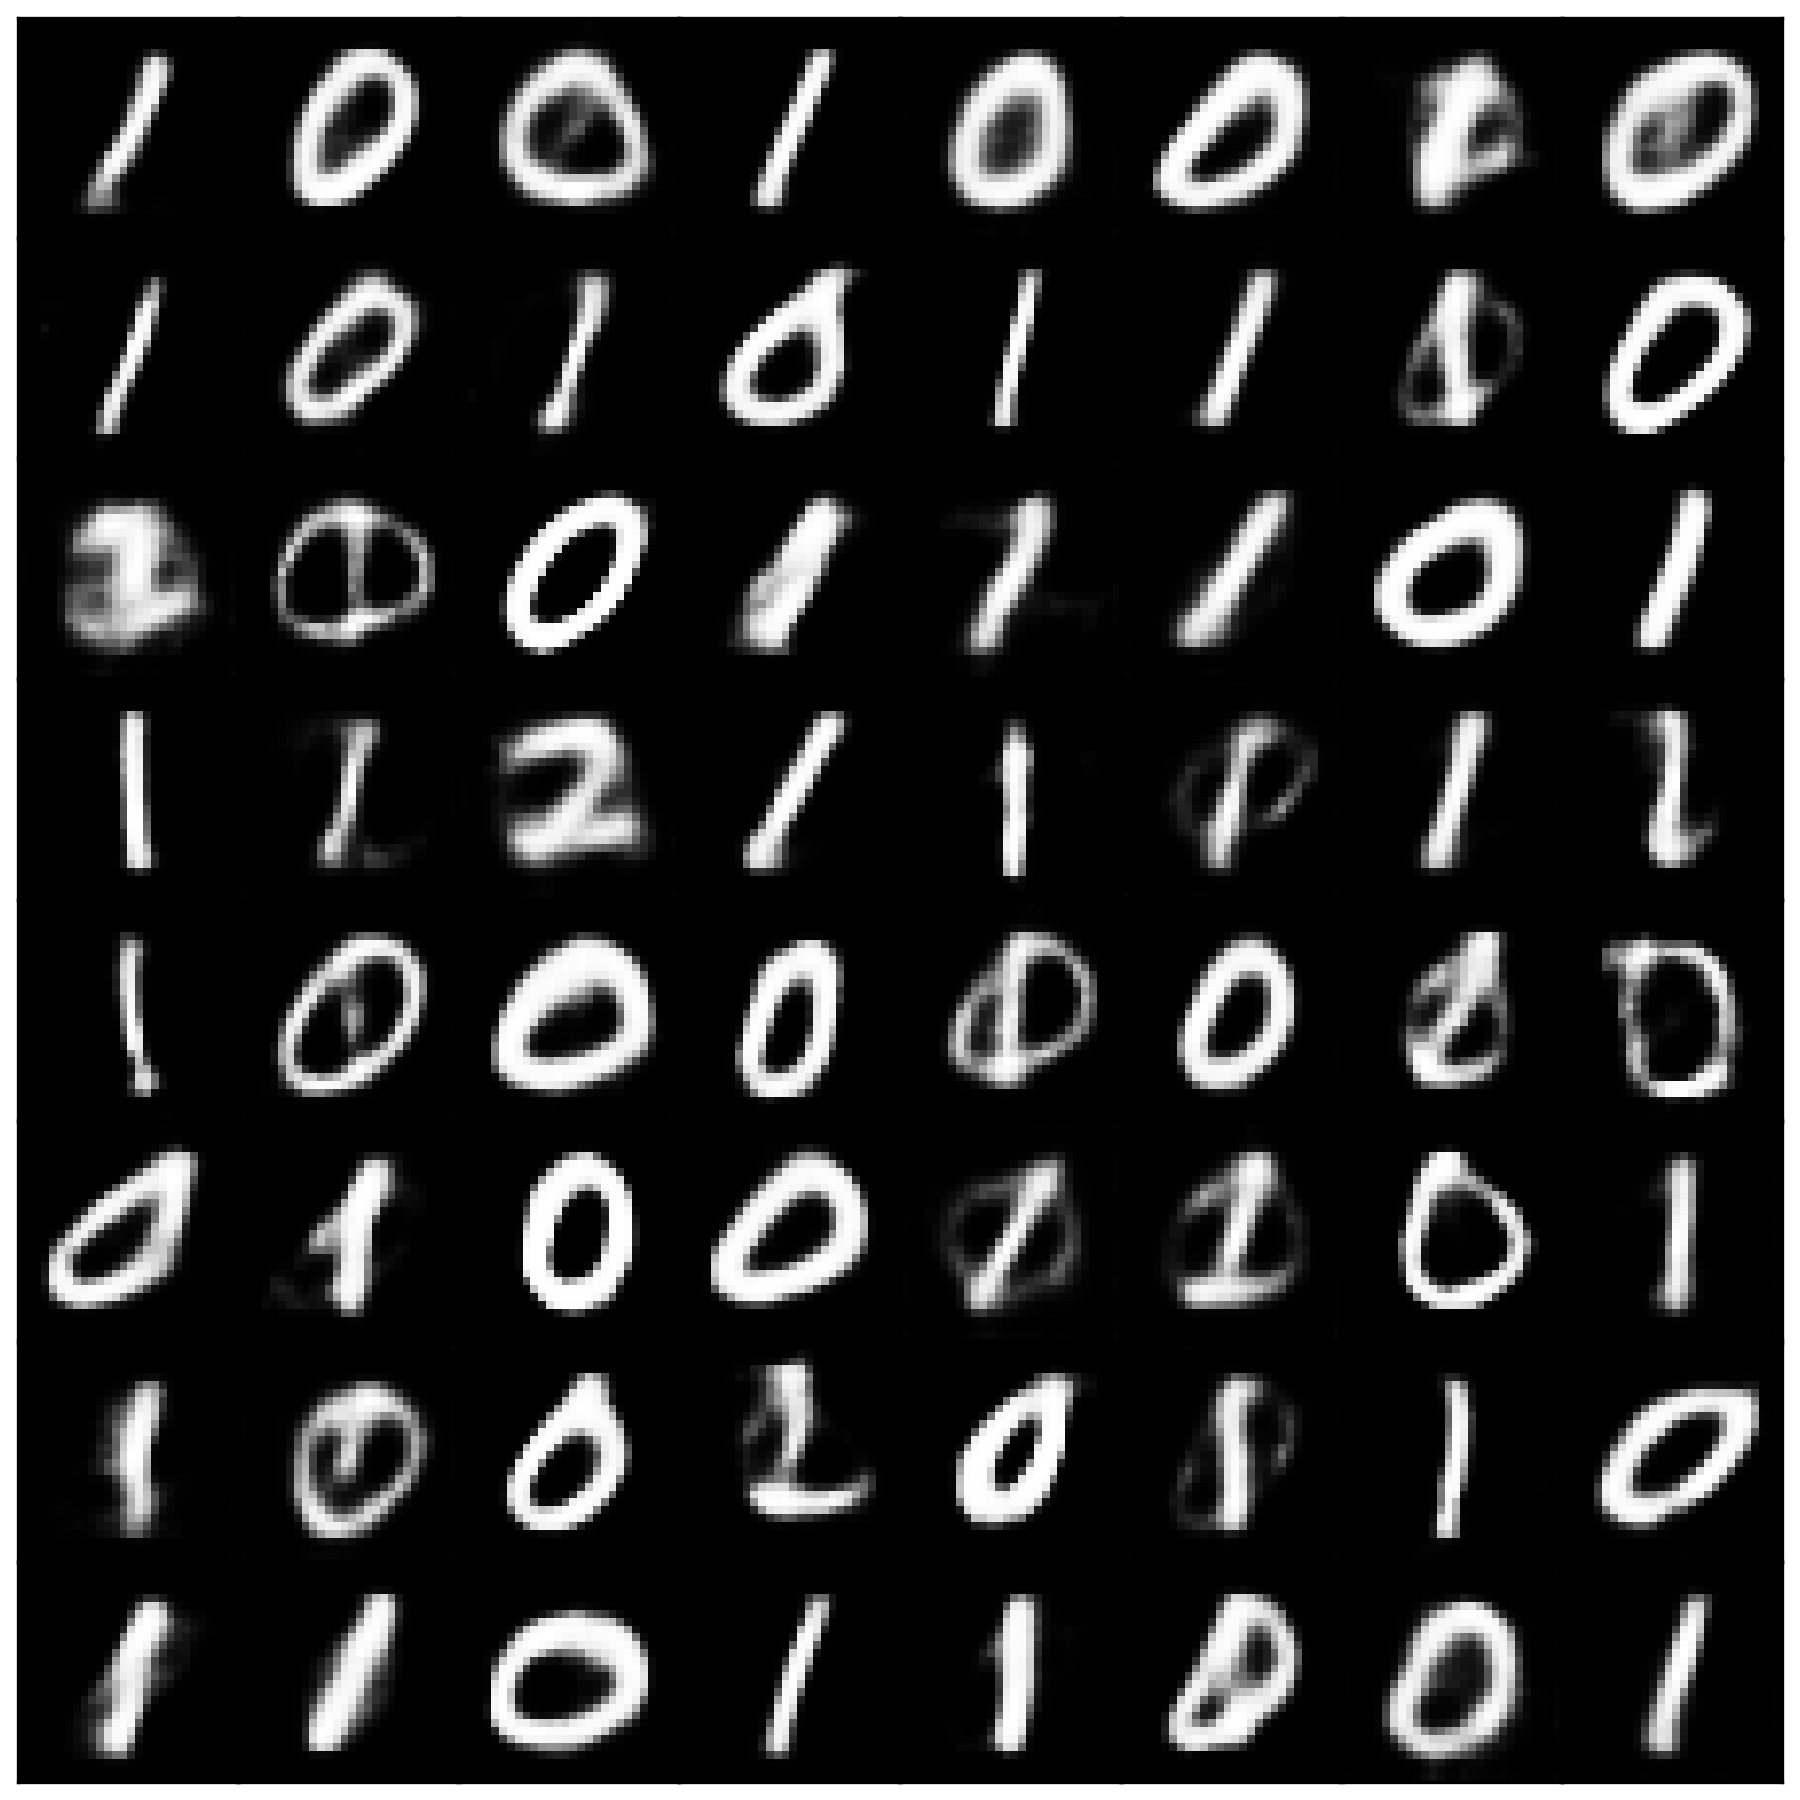
\includegraphics[width=0.9\textwidth]{Figures/PS_v2/vae-ubMNIST012-gensamples.png}
    \end{subfigure}
    \caption{Generated samples from the balanced/unbalanced 012-MNIST dataset by Gen-RKM (first two figures) and VAE (last two figures). The first and the third figures display the generations from a balanced dataset, while the second and the fourth figures show the generations from an unbalanced dataset.}
    \label{fig-mnist}
\end{figure} \cleardoublepage

\chapter[Proposed Methods]{Proposed Methods: Weighted sampling schemes towards diversified generation in Gen-RKM}
\label{chap-methods}
\chaptermark{Proposed Methods}
As discussed in the literature review section, the unbalanced data problem could occur in either supervised or unsupervised scenarios. In this chapter, We propose methods to address the problem within the framework of Gen-RKM under both the two settings.


\section{Mitigating data imbalance in supervised setting}
\label{sec-methods-supervised}
Normally, classic strategies like class re-sampling or re-weighting (cost-sensitive training) can both be applied to address data imbalance issues in supervised learning settings. However, in the context of the unique architecture of Gen-RKM, where the final latent space is derived by performing SVD on the entire training dataset following the acquisition of the feature map and pre-image map, the re-weighting approach is ineffective. This is because re-weighting on the RKM loss function only affects the weights of the feature map and pre-image map via backpropagation, and does not impact the final SVD process. Consequently, re-sampling methods are primarily investigated in this context.

\subsection{Inverse frequency sampling}
Consider a training dataset $\bD_{\text{train}} = \{ (\bx_i, \by_i) \}_{i=1}^N$, where $(\bx, \by)$ is the pair of feature and target, $\bx_i$ the feature vector of the $i$th sample, $\by_i \in (0, 1)^c$ the corresponding one-hot target vector over $c$ classes, and $N$ the number of samples in the training set. The sampling weights can be obtained simply by calculating the reciprocal of the frequency of the target classes: $w_i = 1/\text{count}(\by_i)$. The sampling probability is, therefore, $p_i=w_i/\sum_{i=1}^N w_i$. Instead of uniformly sampling data from the training set during the training phase, data points from the minor classes would be sampled with a higher probability than those from the major classes. Therefore, the distribution of training data is modified to achieve a more balanced representation across all classes.

\subsection{Inverse frequency sampling in the framework of Gen-RKM}
The detailed sampling procedure based on inverse frequency sampling in Gen-RKM is illustrated in this subsection. Although inverse frequency sampling is the most classic and straightforward method, adjustments are necessary when applying it to Gen-RKM due to the model’s unique architecture. Since the final step of RKM training requires an SVD on the full training set to obtain the latent space, re-sampling is not only needed at the beginning of every mini-batch but also before the last SVD step on the full training set. The detailed training step is shown below in algorithm \ref{alg-invs-rkm}.
\begin{algorithm}[H]
\caption{inverse frequency sampling for one-view Gen-RKM (Dual)}
\label{alg-invs-rkm}
\begin{algorithmic}[1]
\Require training data $\bD = \{\bx_i, \by_i\}_{i=1}^{N}$; mini-batch size $m$; \\
regularization parameters $\eta, c_{\text{stab}}, \gamma$; \\
explicit feature map $\bphi_{\boldsymbol{\theta}}(.)$ and explicit pre-image map $\bpsi_{\boldsymbol{\zeta}}(.)$; \\
dimension of latent space $s$;
\LComment{Compute Inverse weight}
\State $w_i \gets \frac{1}{count(\by_i)}$ \Comment{the reciprocal of the frequency of $\by_i$}
\State $p_i \gets w_i / \sum_{i=1}^n w_i$
\LComment{Training loop}
    \For{each epoch}
        \For{each mini-batch}
        \State $B \gets$ sample a mini-batch of size $m$ with probability $\boldsymbol{x}_i \sim p_i$ 
        \State do step 6-11 in algorithm \ref{alg-gen-rkm-dual}
        \EndFor
    \EndFor
\LComment{Final step to get all latent variables on modified full dataset}
\State $\bD_{\text{resampled}} \gets$ resample a size $N$ dataset from $\bD$ with probability $\bx_i \sim p_i$ 
\State repeat step 7-9 in algorithm \ref{alg-gen-rkm-dual}  on $\bD_{\text{resampled}}$
\end{algorithmic}
\end{algorithm}


\subsection{Extension to conditional generation in Gen-RKM}
\label{subsec-methods-congen}
Conditional generation involves generating new data samples based on certain attributes. A ubiquitous technique in combating data imbalance is the use of conditional generation with deep generative model. By learning the underlying data distribution via deep architecture, one can augment minority modes (or classes) with highly realistic synthetic data. Both VAE and GAN have their own modified version for conditional modeling, known as CVAE\cite{sohnLearningStructuredOutput2015} and CGAN\cite{mirzaConditionalGenerativeAdversarial2014}, respectively. However, the implementation of conditional generation within the framework of Gen-RKM has not yet been explored. Here, We propose a simple yet effective modified generation procedure aimed at achieving structured output representation in Gen-RKM ,as outlined in algorithm \ref{alg-con-gen-rkm}.

Let $\bH$ as a collection of latent variables and $\bY$ as the corresponding class labels for each data point. Recall that generation is based on random sampling from a trained GMM on latent variables in vanilla Gen-RKM:
\begin{equation}
    \bh^{*}\sim p(\bh) = \sum_{k=1}^{l}\pi_k\Normal(\bh | \bmu_{\bh,k},\bSigma_{\bh,k}).
\end{equation}
Instead of fitting GMM merely on $\bH$, we consider modeling the joint PDF of $\bh$ and $\by$ on a concatenated matrix : $\bH_{cat} = [\bH^\top; \bY^\top]^\top$. To obtain the generation conditioned on a certain class label, it is natural to sample from the conditional distribution $p(\bh|\by)$. One can verify that the conditional distribution of a mixture of Gaussian results in another GMM :
\begin{equation}
    p(\bh | \by) = \sum_{k=1}^{l}\pi_k^{\prime}\Normal(\bh | \bmu_{\bh|\by,k},\bSigma_{\bh|\by,k}).
\end{equation}
with the updated weights for each Gaussian component,
\begin{equation}
    \pi_k^{\prime} = \frac{\pi_k \Normal(\by|\bmu_{\by,k},\bSigma_{\by\by,k})}{\sum_{v=1}^{l}\pi_{v}\Normal(\by | \bmu_{\by,v},\bSigma_{\by\by,v})}.
\end{equation}
The more detailed derivation is shown in appendix \ref{A-conGMM}.
% Recall that the vanilla generation procedure in Gen-RKM is based on random sampling from a trained GMM on latent variables. 
\begin{algorithm}[H]
\caption{Conditional generation algorithm in Gen-RKM}
\label{alg-con-gen-rkm}
\begin{algorithmic}[1]
    \Require trained explicit pre-image map $\bpsi_{\boldsymbol{\zeta}}(.)$, interconnection matrix $\bW$; \\
    latent variables $\bH = [\bh_1,\dots,\bh_N] \in \bbR^{d\times N}$; \\
            class labels for each data point $\bY = [\by_1,\dots,\by_N] \in \bbR^{c\times N}$ (in one-hot encoding form, $c$ is the number of classes);\\
            conditioned class label $\by \in \bbR^{c}$ (in one-hot encoding form);\\
            number of Gaussian components in GMM $l$;
    \State $\bH_{cat} \gets [\bH^\top; \bY^\top]^\top \in \bbR^{(d+c)\times N}$
    \State $p(\bh,\by) \gets \text{GMM}_{l}(\bH_{cat})$
    \State $\bh^* \sim p(\bh|\by)$
    \State $\bx_{\text{gen}} \gets \bpsi_{\boldsymbol{\zeta}}(\bW \bh^{*})$
\end{algorithmic}
\end{algorithm}

This modification is inspired by the observation that, in the latent space, the latent variables of different class labels tend to cluster together, as shown in Figure \ref{fig-latent-ub}. Therefore, if we can sample from a selected sub-cluster, we are able to generate data conditioned on a particular label. Notice that this algorithm will fail if latent variables with different labels are intermixed in the latent space. It is advised to include label information as the second view in the training phase before conditional generation because latent representation would become more separated based on their categories, as pointed out in \cite{pandeyGenerativeRestrictedKernel2021}.


\section{Mitigating data imbalance in unsupervised setting}
\label{sec-methods-unsupervised}
Generative learning is typically conducted under an unsupervised manner, which means no label information is involved during the learning process. However, data imbalance problem might still exist even though it is hard to be clearly identified. More specifically, regions of the data space with fewer data points might be overlooked in the generative model, resulting in biased or unfair generation.  Inspired by the successful implementation of ridge leverage scores (RLS) sampling in combating mode collapse problem in GAN \cite{schreursLeverageScoreSampling2022}, we propose to incorporate the RLS sampling as a diversity sampling technique within the framework of Gen-RKM when label information is not available. The basic theoretical aspects of RLS and the modified training algorithm based on RLS sampling will be discussed below

\subsection{Ridge leverage score sampling}
Given a data matrix $\bX = [\bx_1,\dots,\bx_N]$ with size $d\times N$, the classical leverage score for the $i$th data point is defined as the $i$th diagonal element value of the projection matrix of $\bX$:
\begin{equation}
    l_{i} = \bx_i^\top (\bX\bX^\top)^{-1}\bx_i.
\end{equation}
Leverage score measures the importance or the influence of an individual observation within the dataset. Historically, it has been widely used for model diagnostics and assessment in classical regression models. Ridge regression is a penalized version of linear regression by including an additional L2 regularization term into the loss objective, its corresponding ridge leverage score for the $i$th observation is given by  
\begin{equation}
    l_{i}^{R}(\gamma) = \bx_i^\top (\bX\bX^\top + \gamma\mathbf{I})^{-1}\bx_i
\end{equation}
where $\gamma > 0$ is known as the regularization parameter in ridge regression. The additional regularization term $\gamma\mathbf{I}$ serves as stabilizing the ill-posed inversion problem in the above expression. Ridge regression can be readily integrated with kernel methods, which is essentially a simplified version of support vector regression \cite{vovkKernelRidgeRegression2013}. Given a feature map $\bvarphi(.)$ with its corresponding similarity metric $K(x,y)=\bvarphi(x)^\top\bvarphi(y)$, the leverage scores of kernel ridge regression can be expressed in a primal-dual form:
\begin{equation}
l_{i}^{KR}(\gamma) = 
    \begin{cases} \text{Primal:} \quad
\bvarphi(\bx_i)^\top(\bS_{\bvarphi}+\gamma\mathbf{I})^{-1}\bvarphi(\bx_i) 
\\
\text{Dual:} \quad
(\bK_{\bvarphi}(\bK_{\bvarphi}+\gamma\mathbf{I})^{-1})_{ii}
    \end{cases}
\end{equation}
Where $\mathbf{K}$ is the gram matrix with respect to similarity metric $K(.,.)$ and $\mathbf{S}_{\bvarphi} = \sum_{i=1}^{N}\bvarphi(\bx_i)\bvarphi(\bx_i)^\top$ is proportional to the sample covariance matrix. Depending on different data sizes and feature map dimensions, one can choose to leverage either primal or dual form to ensure optimal computational efficiency. 

In addition to a regression model diagnostic tool, RLS is crucial for sampling diverse landmarks in low-rank approximation problems, e.g., Nystr\"{o}m approximation for kernel matrices \cite{fanuelDiversitySamplingImplicit2021, mccurdyRidgeRegressionProvable2018}.  Schreurs et al. also illustrate the effectiveness of implementing RLS sampling in mitigating generation biases brought by unbalanced training data in the framework of GAN \cite{schreursLeverageScoreSampling2022}. Once the leverage scores are computed, one can immediately deduce the sampling probability for each data point via normalization on the leverage scores: $p_i = l^{KR}_i / \sum_{j=1}^N l^{KR}_j$. Ideally, minority modes tend to have higher leverage scores, making these points more likely to be oversampled, resulting in a more uniform-like distribution of the resampled data. A motivating example is presented in figure \ref{rls-demo}. One can observe that samples from minority modes generally share higher RLSs and the RLSs for the majority group are very close to zero, thus RLS sampling could automatically oversample minority modes while data points from the majority group are downsampled. In this spirit, problem of imbalance could be resolved by RLS sampling.

\begin{figure}[ht]
    \centering
    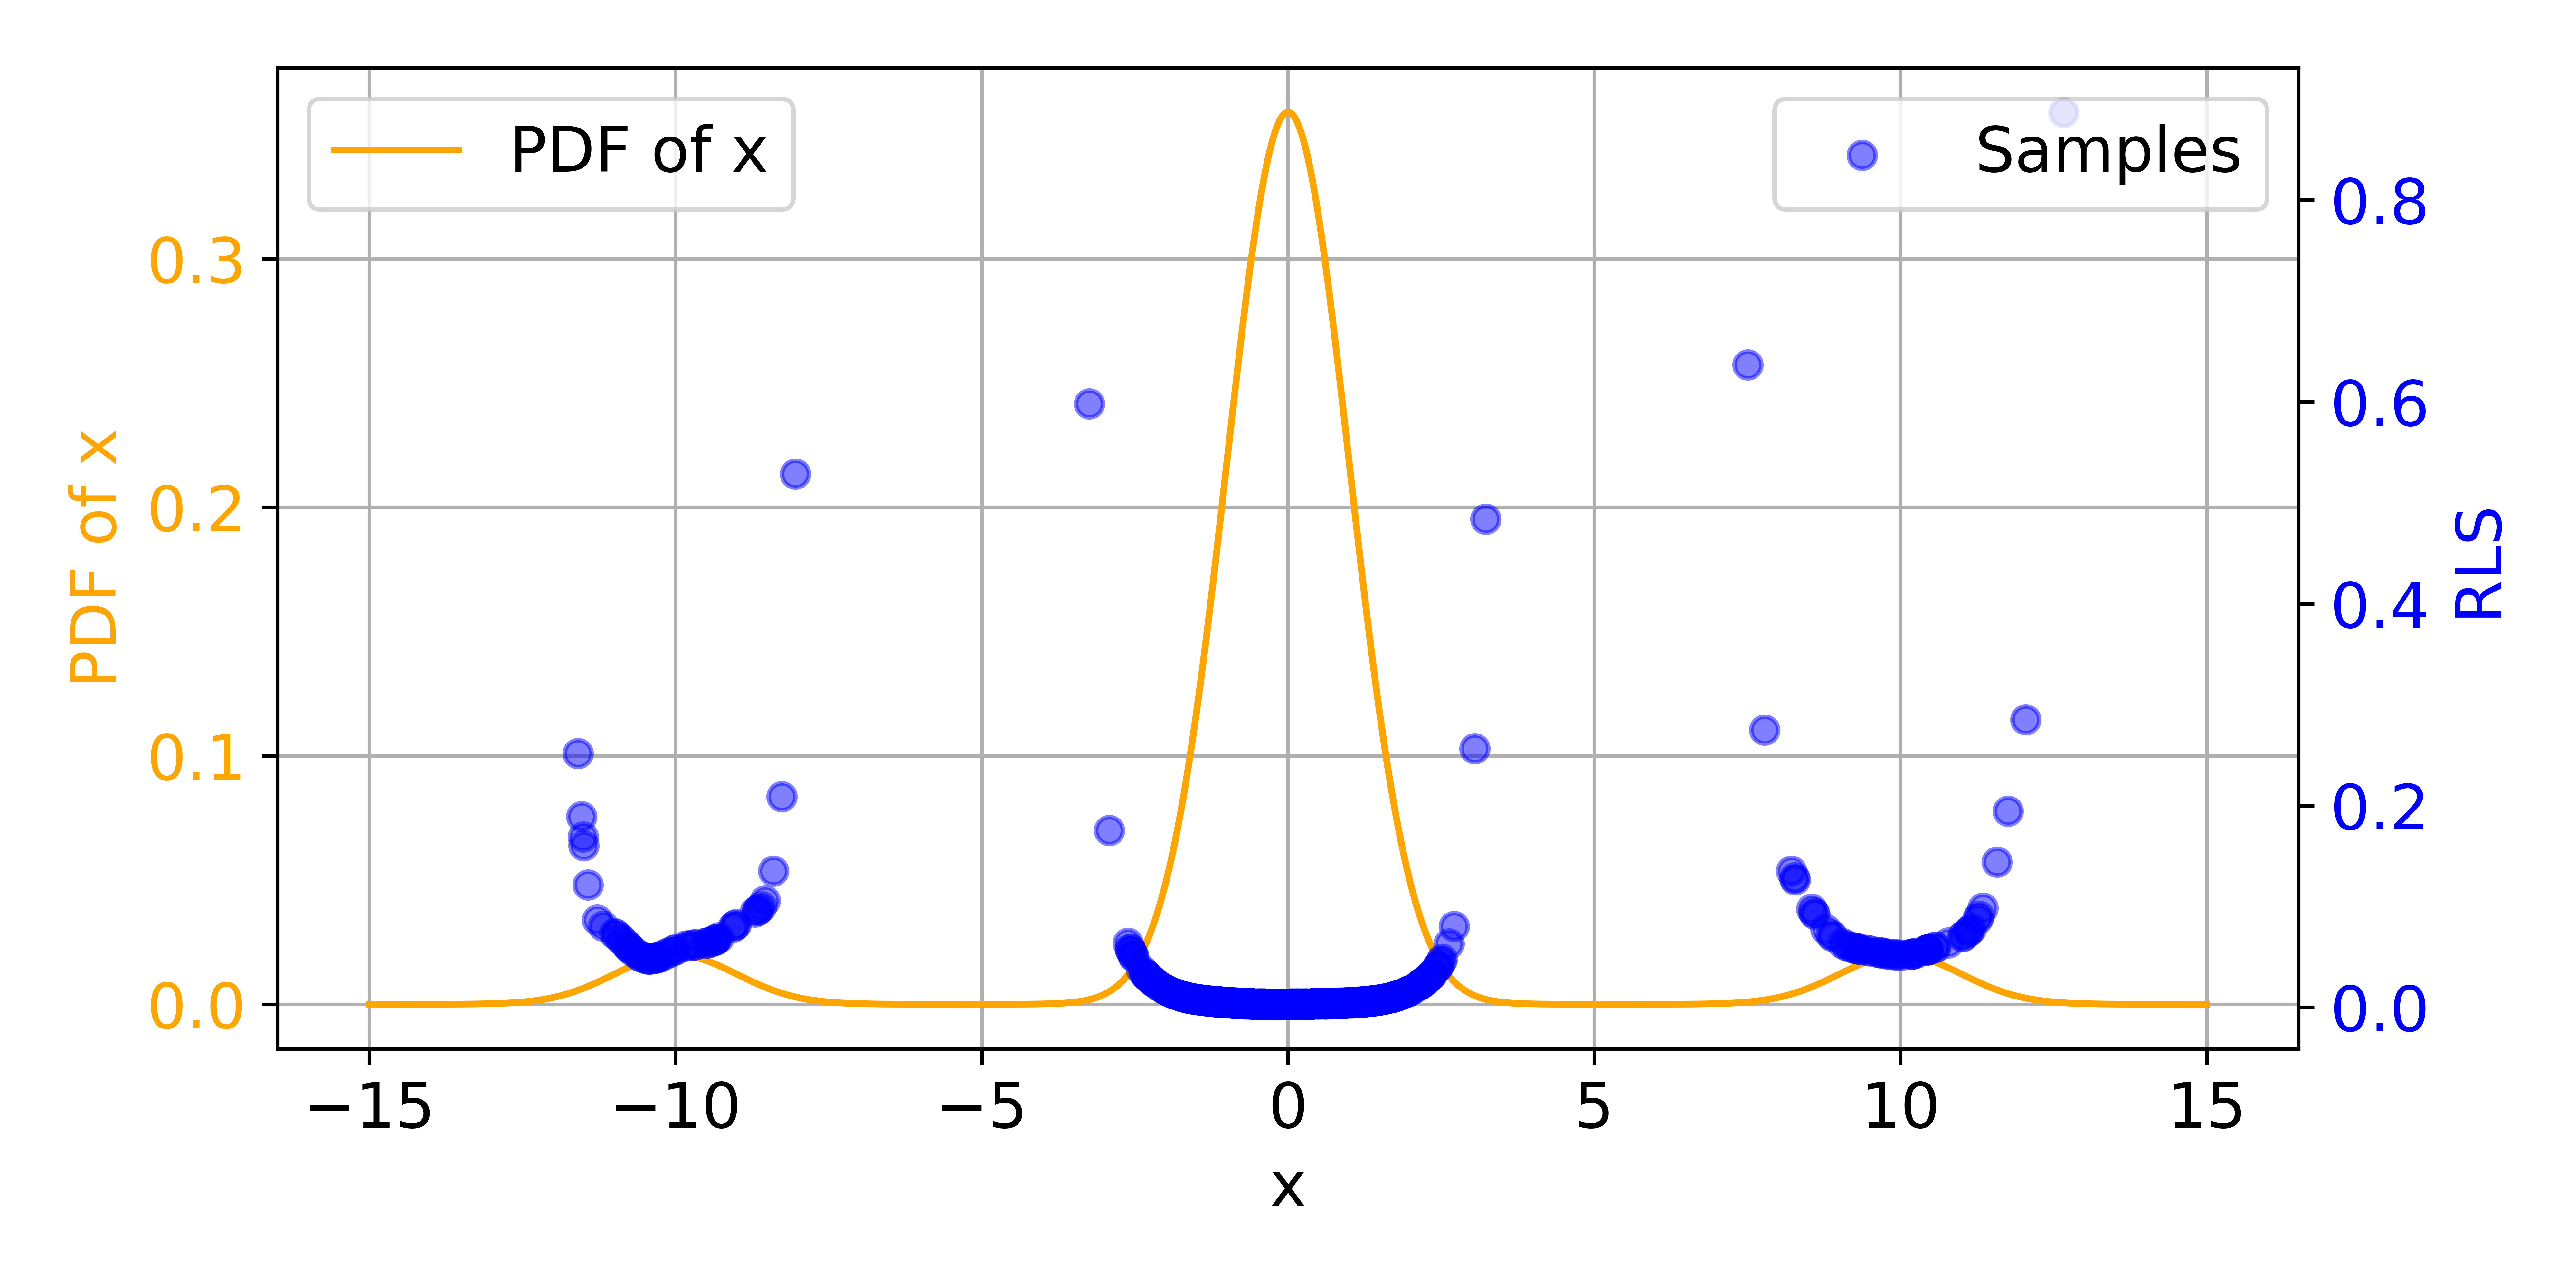
\includegraphics[width=0.8\linewidth]{Figures/Methods/rls-demo.png}
    \caption{A toy example illustrates using RLS sampling can help capture minority modes in the data. The orange curve depicts the PDF of a Gaussian mixture distribution with 1 majority mode in the middle and 2 minority modes on two sides, where the PDF is defined as $p=0.05\caN(-10,1) + 0.9\caN(0,1) + 0.05\caN(10,1)$. Blue points are a collection of random samples from that pdf, where the height of each point corresponds to the RLS for that individual point. RLSs are computed based on a Gaussian kernel with $\gamma=10^{-3}$ and $\sigma=3$. One can observe that samples from minority modes generally have higher RLSs, thus sampling based on the RLSs could contribute to balance the data. This figure is reproduced from \cite{schreursLeverageScoreSampling2022}.}
    \label{rls-demo}
\end{figure}

\subsection{Incorporating RLS sampling within the framework of Gen-RKM}
\label{subsec-methods-incor-rls-with-Genrkm}
The detailed sampling procedure based on RLSs in Gen-RKM is illustrated in this subsection. The main methodology is primarily developed based on \cite{schreursLeverageScoreSampling2022}, with some modifications applied due to differences in the model setting. We start by discussing two possible options for feature maps of RLS sampling in the framework of Gen-RKM.

\noindent\textbf{Feature map choices }\ To compute RLSs, a feature map function needs to be defined beforehand. Considering our work mostly focuses on learning image data, a more sophisticated similarity metric, typically a deep neural network, is preferred. Here we consider two different approaches for constructing feature maps.
\begin{itemize}
    \item \textbf{Shared explicit feature map with Gen-RKM: } Both Gen-RKM and RLS sampling are kernel based methods, meaning that they each have a feature map function projecting training data into feature space. Therefore the most natural way is to use the encoder part of Gen-RKM directly as feature map in RLS sampling. In this case, computation on RLS and Gen-RKM will share one same explicit feature map network: $\bvarphi(.)=\bphi(.)$ (recall that we denote feature map for Gen-RKM as $\bphi(.)$). This approach is preferred when no prior information is available.
    \item  \textbf{Explicit feature map based on a pre-trained classifier: } Another possible option is to use the next-to-last layer of a pre-trained classifier, such as ResNet18\cite{heDeepResidualLearning2016}, as the feature extractor. Similar ideas are proposed in \cite{schreursLeverageScoreSampling2022, zhangDeterminantalPointProcesses2017a}, where weighted sampling schemes are conducted based on the embeddings extracted from a pre-trained classifier. Some popular deep neural network models pre-trained on ImageNet\cite{dengImageNetLargescaleHierarchical2009} are readily implemented in \texttt{PyTorch} and \texttt{TensorFlow}. Notice that there is no need to fine-tune the pre-trained model on the exact training dataset, only forward pass operation is required to get image embeddings.
\end{itemize}

\noindent\textbf{Techniques for dimension reduction }\ Modern deep neural networks are characterized by their high dimensionality. For example, the output dimension of the next-to-last layer in AlexNet\cite{krizhevskyImageNetClassificationDeep2012} is 4096. Computation on RLSs can be rather demanding when the dimension of feature space is large. To improve computational efficiency, we introduce two dimension reduction techniques for different feature choices, as suggested in \cite{schreursLeverageScoreSampling2022}.
\begin{itemize}
    \item \textbf{Gaussian sketching: }\ Gaussian sketching is a ubiquitous approach in low-rank approximating large matrices in the field of randomized linear algebra. Let $\bZ$ be a Gaussian random matrix of size $d\times k$ where $k << d$, and $\bvarphi(\bX_{b})$ be a mini-batch of data with size $m$ after feature map in RLS sampling. The sketched matrix is simply given by multiplying the random matrix: 
    \begin{equation}
        \widetilde{\bvarphi}(\bX_{b}) = \bZ^{\top}\bvarphi(\bX_{b})\in \bbR^{m\times k}.
    \end{equation}
    This random projection guarantees that pairwise distances in the dataset are preserved in a much lower embedding space according to Johnson-Lindenstrauss lemma \cite{schreursLeverageScoreSampling2022}. One can refer to \cite{woodruffSketchingToolNumerical2014} for more technical details about sketching methods.
    \item \textbf{UMAP: }\ Uniform Manifold Approximation and Projection (UMAP) is a widely used non-linear dimensionality reduction technique developed by McInnes et al. \cite{mcinnesUMAPUniformManifold2020}. Compared to Gaussian sketching, UMAP can preserve more complex patterns in the data, though its training process is significantly slower.
\end{itemize}

\noindent\textbf{Modified training schemes based on RLS sampling }\ Detailed training algorithms based on RLS sampling are outlined in this subsection. For explicit feature map based on a pre-trained classifier, UMAP is preferred for dimension reduction in this case since RLSs are only computed once before the main training loop. The algorithm essentially follows the same principle as the inverse frequency sampling discussed earlier, i.e. performing weighted sampling under each mini-batch as well as resampling the full dataset for the final computation step, as presented in algorithm \ref{alg-rls-rkm-fixed}. 
\begin{algorithm}[H]
\caption{RLS Sampling in Gen-RKM with explicit feature map based on a pre-trained classifier}
\label{alg-rls-rkm-fixed}
\begin{algorithmic}[1]
\Require training data $\bD = \{\bx_i\}_{i=1}^{N}$; mini-batch size $m$; \\
regularization parameters $\eta, c_{\text{stab}}, \gamma_{RKM}$ for Gen-RKM; \\
explicit feature map $\bphi_{\btheta}(.)$ and explicit pre-image map $\bpsi_{\boldsymbol{\zeta}}(.)$ for Gen-RKM; \\
pre-trained classifier feature map $\bvarphi(.)$ and regularization $\gamma_{RLS}$ for RLS sampling; \\
dimension reduction size $k$
\LComment{Pre-compute RLS}
\State $\{\widetilde{\bvarphi}(\boldsymbol{x}_i)\}_{i=1}^{N} \gets \text{UMAP}_{k}(\{\bvarphi(\boldsymbol{x}_i)\}_{i=1}^{N})$ \Comment{get UMAP embeddings}
\State $l_i \gets \widetilde{\bvarphi}(\boldsymbol{x}_i)^\top(\bS_{\Tilde{\bvarphi}}+\gamma_{RLS}\mathbf{I})^{-1}\widetilde{\bvarphi}(\boldsymbol{x}_i)$ \Comment{Compute leverage scores}
\State $p_i \gets l_i / \sum_{j=1}^n l_j$
\LComment{Training loop}
    \For {each epoch}
        \For{each mini-batch $B \subset \bD$}
        \State $B \gets$ sample a mini-batch of size $m$ with probability $\boldsymbol{x}_i \sim p_i$ 
        \State do step 6-11 in algorithm \ref{alg-gen-rkm-dual}
        \EndFor
    \EndFor
\LComment{Modified final computation step in Gen-RKM}
\State $\bD_{\text{resampled}} \gets$ resample the full dataset with probability $\bx_i \sim p_i$ 
\State repeat step 7-9 in algorithm \ref{alg-gen-rkm-dual}  on $\bD_{\text{resampled}}$
\end{algorithmic}
\end{algorithm}

For the RLS sampling using a shared feature map with Gen-RKM, RLSs are recomputed in each iteration since the feature map for RLS is not fixed (i.e. parameters of feature map network need to be updated with every iteration). To alleviate the computational load, Gaussian sketching is implemented to reduce the dimension of the feature map. Sketching is considerably fast even when performed in every iteration, due to the simplicity of matrix multiplication involved. In addition, a two-stage sampling procedure is applied as suggested in \cite{schreursLeverageScoreSampling2022}. First, a subset of training data is uniformly sampled (we set the size of this subset to be 20 times the mini-batch size), and RLSs are computed only for that core set. In the second stage, a mini-batch is sampled based on the calculated RLSs of this core set for training. The detailed implementation is shown in algorithm \ref{alg-rls-rkm-shared}. Likewise in the previous setting, the final computation step in Gen-RKM is conducted based on the RLS-resampled dataset.
\begin{algorithm}[H]
\caption{RLS Sampling in Gen-RKM with a shared feature map}
\label{alg-rls-rkm-shared}
\begin{algorithmic}[1]
\Require training data $\bD = \{\bx_i\}_{i=1}^{N}$; mini-batch size $m$; \\
regularization parameters $\eta, c_{\text{stab}}, \gamma_{RKM}$ for Gen-RKM; \\
explicit feature map $\bphi_{\btheta}(.)$ and explicit pre-image map $\bpsi_{\boldsymbol{\zeta}}(.)$ for Gen-RKM; \\
regularization parameter $\gamma_{RLS}$ for RLS sampling and dimension reduction size $k$;
\LComment{Training loop}
    \For {each epoch}
        \For{each mini-batch $B \subset \bD$}
        \LComment{two-stage sampling procedure}
        \State $\bD_{s} \gets$ uniformly sample a subset from $\bD$ with size $20*m$ 
        \State $\widetilde{\bphi}_{\btheta}(\bx_i) \gets \bZ_k^\top\bphi_{\btheta}(\bx_i),\quad \text{s.t.}\bx_i\in \bD_s$ \Comment{Gaussian sketching}
        %\LComment{Compute RLS on $\bD_{s}$ under each iteration}
        \State $l_i \gets \widetilde{\bphi}_{\btheta}(\bx_i)^\top(\bS_{\widetilde{\bphi}_{\btheta}}+\gamma_{RLS}\mathbf{I})^{-1}\widetilde{\bphi}_{\btheta}(\bx_i)$
        \State $p_i \gets l_i / \sum_{j=1}^{20m} l_j$
        \State $B \gets$ sample a mini-batch of size $m$ with probability $\bx_i \sim p_i$
        \State do step 6-11 in algorithm \ref{alg-gen-rkm-dual}
        \EndFor
    \EndFor
\LComment{Compute final RLS on full dataset}
\State $\widetilde{\bphi}_{\btheta}(\bx_i) \gets \bZ_k^\top\bphi_{\btheta}(\bx_i),\quad \text{s.t.}\bx_i\in \bD$
\State $l_i^{\text{final}} \gets \widetilde{\bphi}_{\btheta}(\bx_i)^\top(\bS_{\widetilde{\bphi}_{\btheta}}+\gamma_{RLS}\mathbf{I})^{-1}\widetilde{\bphi}_{\btheta}(\bx_i)$
\State $p_i^{\text{final}} \gets l_i^{\text{final}} / \sum_{j=1}^N l_j^{\text{final}}$
\LComment{Modified final computation step in Gen-RKM}
\State $\bD_{\text{resampled}} \gets$ resample a dataset of size $N$ with probability $\bx_i \sim p_i^{\text{final}}$ 
\State repeat step 7-9 in algorithm \ref{alg-gen-rkm-dual}  on $\bD_{\text{resampled}}$
\end{algorithmic}
\end{algorithm}

\subsection{Extension: Other measurement for imbalance sampling}
\label{subsec-methods-islation-forest}
As mentioned in Section \ref{subsec-lr-unbalance-super-unsuper}, many studies focus on anomaly detection in unsupervised learning settings. These experiences can be leveraged to address the issue of imbalanced data within the Gen-RKM framework. In addition to the ridge leverage score, which assesses the importance of individual observations in a dataset, other anomaly detection methods can be utilized to measure the uniqueness or anomaly level of observations. Subsequently, re-sampling can be carried out based on the uniqueness of each sample, similar to the approach used in ridge leverage score sampling. 

Isolation forest (Iforest)\cite{liu2008isolation}, as mentioned in Section \ref{subsec-lr-unbalance-super-unsuper}, provides an assessment for the degree of the anomaly of each data point as follows,
\begin{align}
&S(x, n) = 2^{-\frac{h(x)}{c(n)}}\label{ascore} \\
&c(n) = 2H(n-1) - \frac{2(n-1)}{n} \\
&H(k) = \ln(k) + \xi
\end{align}
where \begin{itemize}
    \item $S(x, n)$ represents the anomaly score of data point $x$, $n$ is the number of samples. The larger the score, the higher the likelihood that $x$ is considered an anomaly or outlier. 
    \item $h(x)$ is the path length required to isolate point $x$ in the isolation forest. Shorter path lengths suggest that $x$ is easier to isolate, thus potentially being an outlier.
    \item $c(n)$ is the average path length under normal conditions for a sample size $n$. This calculation takes into account the balance and imbalance factors of a binary search tree.
    \item $H(k)$  is a harmonic number, typically used to estimate the average path length of binary search trees. And $\xi$ is the Euler-Mascheroni constant, approximately 0.5772156649.
\end{itemize}
We can easily integrate isolation forest anomaly score sampling (Iforest sampling) into the Gen-RKM framework to address the imbalance data problem by simply replacing steps 3-4 in Algorithm \ref{alg-rls-rkm-fixed} with the computation of anomaly scores using an isolation forest model (see $S(x, n)$ in equation \ref{ascore}) based on the extracted features from the feature map,  while maintaining all other steps unchanged. Note that this is only applicable with a pre-trained classifier-based feature map, as it allows the isolation forest to be fitted just once in the algorithm.





\chapter{Experiments and Results}
\label{chap-expr}
In this chapter, various sampling techniques outlined in Chapter \ref{chap-methods} are evaluated within the Gen-RKM framework using both synthetic datasets and real-world datasets. We begin with the basic experiment setup, including the datasets used, evaluation tools, and key hyperparameter settings in Section \ref{sec-expr-setup}. After that, we conducted experiments for both the supervised and unsupervised settings to validate their effectiveness. More specifically, Section \ref{sec-expr-supervised} primarily evaluates the performance of inverse frequency sampling in the supervised setting, while also studying and improving the applicability of conditional generation under unbalanced data. Next, Section \ref{sec-expr-unsupervised} examines the performance of RLS sampling in diversifying generation under the unsupervised manner. In addition, Iforest sampling (i.e., weighted sampling based on anomaly scores outputted from the Isolation Forest algorithm), an extension of RLS sampling, is also included in the comparison. Finally, a series of additional studies are conducted in Section \ref{subsec-additional-studies} to gain full insights into the strengths and weaknesses of our proposed methods. The Python code for the experiment part has been made publicly available on \href{https://github.com/wenjierong1999/Unbalanced-RKM}{GitHub}. 

\section{Experiment set-up}
\label{sec-expr-setup}

\subsection{Datasets}
\label{subsec-expr-datasets}
The following datasets are considered in the experiment part:
\begin{description}[leftmargin=0pt]
   \item[Synthetic ring/grid datasets] Two unbalanced synthetic datasets are generated following the setting in \cite{schreursLeverageScoreSampling2022}: an unbalanced ring with 4 minority modes (Ring) and an unbalanced grid (Grid) with 10 minority modes (shown in Figure \ref{fig-2d} below). Ring is a mixture of eight two-dimensional isotropic Gaussians in the 2D-plane with means $2.5 \times (\cos(\frac{2\pi}{8}i), \sin(\frac{2\pi}{8}i))$ and standard deviation 0.05 for $i\in{ 1, . . . , 8 }$. The probability of sampling from the first 4 consecutive Gaussians is only 0.05 times the probability of sampling from the last 4 modes. Grid is a mixture of 25 two-dimensional isotropic normals with a standard deviation of 0.05 and with means on a square grid with spacing 2. The first rectangular blocks of 2 × 5 adjacent modes are depleted with a factor of 0.05. 2500 samples are generated for each normal mode, thus 125 for each minority mode. 
\begin{figure}[H]
    \centering
    \begin{subfigure}{0.45\textwidth}
        \centering
        
\includegraphics[width=0.8\textwidth]{Figures/Methods/ring_dataset.png}
    \end{subfigure}
    \hfill
    \begin{subfigure}{0.45\textwidth}
        \centering
        
\includegraphics[width=0.8\textwidth]{Figures/Methods/grid_dataset.png}
    \end{subfigure}
    \caption{2D synthetic data: Ring(left) and Grid(right)}
    \label{fig-2d}
\end{figure}

    \item[Unbalanced 012-MNIST/MNIST dataset] For the natural dataset from the real world, we opt to employ MNIST as the first benchmark dataset for evaluating the effectiveness of different weighted sampling schemes. MNIST\cite{lecunGradientbasedLearningApplied1998} contains 60000 images of handwritten digits varying from 0 to 9, where the size of each image is fixed on $28\times 28$ with single color channel. We mainly consider two unbalanced variants of MNIST in our experiments. The first created dataset, namely unbalanced 012-MNIST, consists of only the digits 0, 1 and 2 where digit 2 is the minority class. Imbalance is artificially introduced by (randomly) reducing the number of digit 2 so that the probability of sampling digit 2 is smaller than that of sampling from other digits. The degree of depletion for digit 2 is determined by a specified imbalance ratio (i.e., ratio of the number of samples in minority class to the number of samples in majority class). The second dataset, unbalanced MNIST, consists of all the digits from 0 to 9. The digits 0, 1, 2, 3, and 4 have been selected as the minority classes, and their numbers are reduced as the same fashion in unbalanced 012-MNIST.  

    \item[Unbalanced Fashion MNIST dataset] Considering the relatively simple patterns of MNIST dataset, Fashion MNIST \cite{xiaoFashionMNISTNovelImage2017} is also used in our experiments for a more challenging replacement. Fashion MNIST consists of 60000 images of fashion items (e.g., different types of shoes and clothes) with 10 categories. Likewise in the MNIST setup, all images in Fashion MNIST are gray-scale with size $28\times 28$. Fashion MNIST is generally more complex due to the high variability in shapes and patterns among the images of different real fashion items. The same procedure in the MNIST case is leveraged to create the unbalanced version of Fashion MNIST dataset. Clothing and bag-related categories (T-shirt, Trouser, Pullover, Dress, Coat, Shirt, Bag) are set to minority classes while shoe-related categories (Sandal, Sneaker, Ankle boot) are considered as the majority classes. 
\end{description}


% For experiments on MNIST datasets, two unbalanced datasets out of MNIST are created. The first created dataset, unbalanced 012-MNIST, consists of only the digits 0, 1 and 2. The digit 2 is chosen as the minor class so that the probability of sampling 2 is smaller ($0.05p$, $0.10p$ and $0.30p$, $p$ is the sampling probability of majority classes) than that of sampling from the digit 0 or 1. The second dataset, unbalanced MNIST, consists of all the digits from 0 to 9. The digits 0, 1, 2, 3, and 4 have been selected as the minority classes, and their sampling probabilities are consistent with the minority class, digit 2, in the unbalanced 012-MNIST dataset.  


\subsection{Evaluation process \& metrics}
As for the evaluation part, 10k samples are randomly generated by each trained model. For the 2D synthetic datasets, valid samples are defined within 3 standard deviations of the nearest modes. A mode is covered by a certain model if there are at least 50 valid generated samples within 3 standard deviations of the mode's center. For image-based datasets, a well-trained classification model is employed to identify the labels of generated samples. Since our objective is to assess both the diversity and quality of the generated samples by different models, the following evaluation metrics are leveraged in our experiment.
\begin{description}[leftmargin=0pt]
    \item[Number of generated samples per mode] We measure mode coverage by counting the number of generated samples under each mode based on the prediction from a trained classifier. Ideally, the distribution of samples per mode should be close to a uniform distribution, which indicates each mode is well captured even though unbalanced training data is given. 

    \item[KL score] A follow-up metric, namely KL score, can be calculated based on the predicted labels of generated samples. KL score is obtained by computing the Kullback–Leibler (KL) divergence between the distribution of the classified labels from the generated samples with a balanced label distribution. We consider KL score as the primary metric to quantify the deviation of the label distribution of the generated samples from a uniform distribution. In the best case, KL score should be very close to zero indicating a balanced generation is acquired. This metric is widely used in various works related to addressing mode collapse problem in GANs \cite{schreursLeverageScoreSampling2022, anaissiDamageGANGenerative2024, yuInclusiveGANImproving2020, demeulemeesterBuresMetricGenerative2021}.

    \item [FID] So far, the above two metrics are both label-based, which means they merely measure the imbalance under the class level. However, the imbalance could occur in both inter-class and intra-class. Additionally, a well-balanced generation does not necessarily ensure results with high quality. For example, the patterns of the generated samples could be highly diverse, but the overall generation could be considered poor quality due to blurriness, weird distortions, and incorrect proportions. Therefore, we propose to employ Fr\'{e}chet Inception Distance (FID) \cite{heuselGANsTrainedTwo2017} as a supplementary evaluation tool for assessing both the diversity and quality of generated images. The nature of FID is to measure the similarity between the distributions of real data and generated data. To compute FID, a pre-trained classifier (normally we use inception-V3) is implemented to extract features of image data, FID is then given by the Fr\'{e}chet distance of two Gaussian distributions: 
    \begin{equation}
        \text{FID} = \| \bmu_r - \bmu_g \|^2 + \text{Tr}(\bSigma_r + \bSigma_g - 2(\bSigma_r \bSigma_g)^{1/2})
    \end{equation}
    where $\bmu_r,\bmu_g$ are the means and $\bSigma_r,\bSigma_g$ are the covariance matrices of extracted embedding of real and generated images, respectively. The reference statistics (i.e., $\bmu_r, \bSigma_r$) are computed based on the (class) balanced dataset in all experiments. A low FID score implies that the distribution of generated images closely matches the distribution of balanced training samples, indicating a more diverse and higher-quality generation.
    
\end{description}


% In the model evaluation part, 10k samples are generated by each trained model. For MNIST-related generation, a pre-trained classification model (resnet18 trained up to 99.43\% accuracy) is used to classify the generations. Since our objective is to improve the diversity of the generated samples under unbalanced input conditions, besides descriptive statistics, KL divergence (Kullback–Leibler divergence) is used as the primary metric to measure the deviation of the distribution of the generated samples from a uniform distribution. And FID (Frechet Inception Distance score) is used to measure the quality of the generated samples (for MNIST-related and Fashion MNIST datasets). For the 2D synthetic datasets, valid samples are defined within 3 standard deviations of the nearest modes. A mode is covered by a certain model if there are at least 50 valid generated samples within 3 standard deviations of the mode's center. 

\subsection{Hyperparameter details}
\label{subsec-setup-hyperparameter}
In this section, we outline the key hyperparameters used in the experiment part. Unless otherwise specified, the hyperparameter settings used in the subsequent experiment part will default to those mentioned below.
\begin{description}[leftmargin=0pt]
    \item[Hyperparameters for Gen-RKM ] The basic hyperparameter settings for training Gen-RKM is displayed in Table \ref{tab-Gen-RKM-setting}. We generally follow the same configurations as those in \cite{pandeyGenerativeRestrictedKernel2021}, except that we slightly increase the dimension of the feature map and the mini-batch size. Considering our experiments required re-training the models multiple times, and the sizes of used datasets are relatively large. To maintain more computationally efficient training, Gen-RKM is computed in the primal form across all our experiments (i.e., eigen-decomposition on the covariance matrix), which necessitates $d_f < m$ to guarantee that the covariance matrix is full rank for more stable computations \cite{pandeyGenerativeRestrictedKernel2021}.
    \begin{table}[ht]
\centering
\begin{tabular}{>{\raggedright\arraybackslash}m{8cm} >{\centering\arraybackslash}m{2cm} >{\centering\arraybackslash}m{2cm} >{\centering\arraybackslash}m{2cm}}
\toprule
\multirow{2}{*}{Hyperparameter} & \multicolumn{3}{c}{Dataset} \\
\cmidrule(lr){2-4}
 & 2D Ring/Grid & 012-MNIST  & MNIST/Fashion \\
\midrule
regularization parameters: $\{\eta,c_{\text{stab}},\gamma_{\text{RKM}}\}$ & \{1;1;100\} & \{1;1;100\}  & \{1;1;100\}  \\
dimension of feature map: $d_f$ & 128 & 300 &300 \\
dimension of latent space: $s$ & 8/25 & 10 & 10 \\
mini-batch size: $m$ & 256 & 328 & 328 \\
maximum epoch number: $N_{\text{epoch}}$ & 150 & 100 & 150\\
number of Gaussian components in GMM: $l$ &8/25 & 3 & 10 \\
learning rate & 0.0001 & 0.0001 & 0.0001 \\
\bottomrule
\end{tabular}
\caption{Hyperparameter settings for Gen-RKM}
\label{tab-Gen-RKM-setting}
\end{table}


    \item[Neural network architectures] The detailed neural network architectures for the feature map and the pre-image map in Gen-RKM are summarized in Table \ref{tab-network-architecture}. For 2D synthetic data, the architecture includes 3 fully connected layers with ReLU activation functions in between. For MNIST-related datasets, the architecture consists of 2 convolutional layers, and ReLU activations are implemented similarly.
    \begin{table}[ht]
\centering
\begin{tabular}{lccc}
\toprule
\multirow{2}{*}{Dataset} & \multirow{2}{*}{Input size} & \multicolumn{2}{c}{Architecture} \\
\cmidrule(lr){3-4}
 & & Feature map & Pre-image map \\
\midrule
2D Ring/Grid & $2$ & \makecell{FC 32 (Linear)\\ ReLu($\alpha=0.2$) \\ FC 64 (Linear) \\ ReLu($\alpha=0.2$) \\ FC 128 (Linear) } &  reverse of fm \\
\midrule
012-MNIST/MNIST/Fashion& $28\times 28\times 1$ & \makecell{Conv $32\times 4\times 4$\\ReLu($\alpha=0.2$) \\ Conv $64\times 4\times 4$ \\ ReLu($\alpha=0.2$) \\ FC 300 (Linear)}   & reverse of fm   \\


\bottomrule
\end{tabular}
\caption{Details of network architectures used in Gen-RKM. All convolutional layers and transposed convolutional layers have stride 2 and padding 1. Pre-image map is the reverse of feature map architecture, except that a sigmoid activation function is implemented for the output layer \cite{pandeyGenerativeRestrictedKernel2021}.}
\label{tab-network-architecture}
\end{table}


    \item[Hyperparameters for RLS sampling] Regarding the hyperparameters used in RLS sampling, we generally adopt the same settings as in the original work of RLS-GAN \cite{schreursLeverageScoreSampling2022}. More specifically, the ridge regularization parameter is set to 0.0001, and feature maps in kernel ridge regression are reduced to $k=25$ by either UMAP or Gaussian sketching. However, Instead of using Inception-v3 as mentioned in \cite{schreursLeverageScoreSampling2022}, we empirically observe that RLS sampling with an explicit feature map based on AlexNet could achieve better performance. Therefore, throughout the experiments, the pre-trained classifier-based RLS sampling is computed using the embeddings extracted from the next-to-the-last layer of Alexnet (which has already been pre-trained on the ImageNet dataset). One can refer to Section \ref{subsec-additional-studies} for the detailed results of the ablation study on the impact of different pre-trained classifiers on the performance of RLS sampling.

    \item[Hyperparameters for Iforest sampling] Fine-tuning the parameters in Isolation Forest is challenging and typically requires some labeled data for validation. However, since no prior information regarding labels is provided in a fully unsupervised manner,  we use the default hyperparameter settings provided in the \href{https://scikit-learn.org/stable/modules/generated/sklearn.ensemble.IsolationForest.html}{\texttt{sklearn}} package.
\end{description}



\section{Experiments on inverse frequency sampling under supervised setting}
\label{sec-expr-supervised}

\subsection{Unbalanced MNIST/Fashion MNIST}
Given that inverse frequency sampling transforms the input distribution into a uniform one, there’s a definite and notable improvement in the diversity of the generated samples. Figure \ref{dis-ub09} shows the distributions of the generated samples from Gen-RKM and Gen-RKM with inverse frequency sampling using MNIST and Fashion MNIST datasets respectively. The minority classes are shown in red and the normal classes are in blue. The improvement in generation diversity is notable. Figures \ref{fig-ub09} visualizes the random generation of Gen-RKM using the MNIST and FashionMNIST datasets, before and after applying inverse frequency sampling. In these figures, the minority classes are highlighted with red rectangles. 

\begin{figure}[H]
    \centering
    \begin{subfigure}{0.45\textwidth}
        \centering
        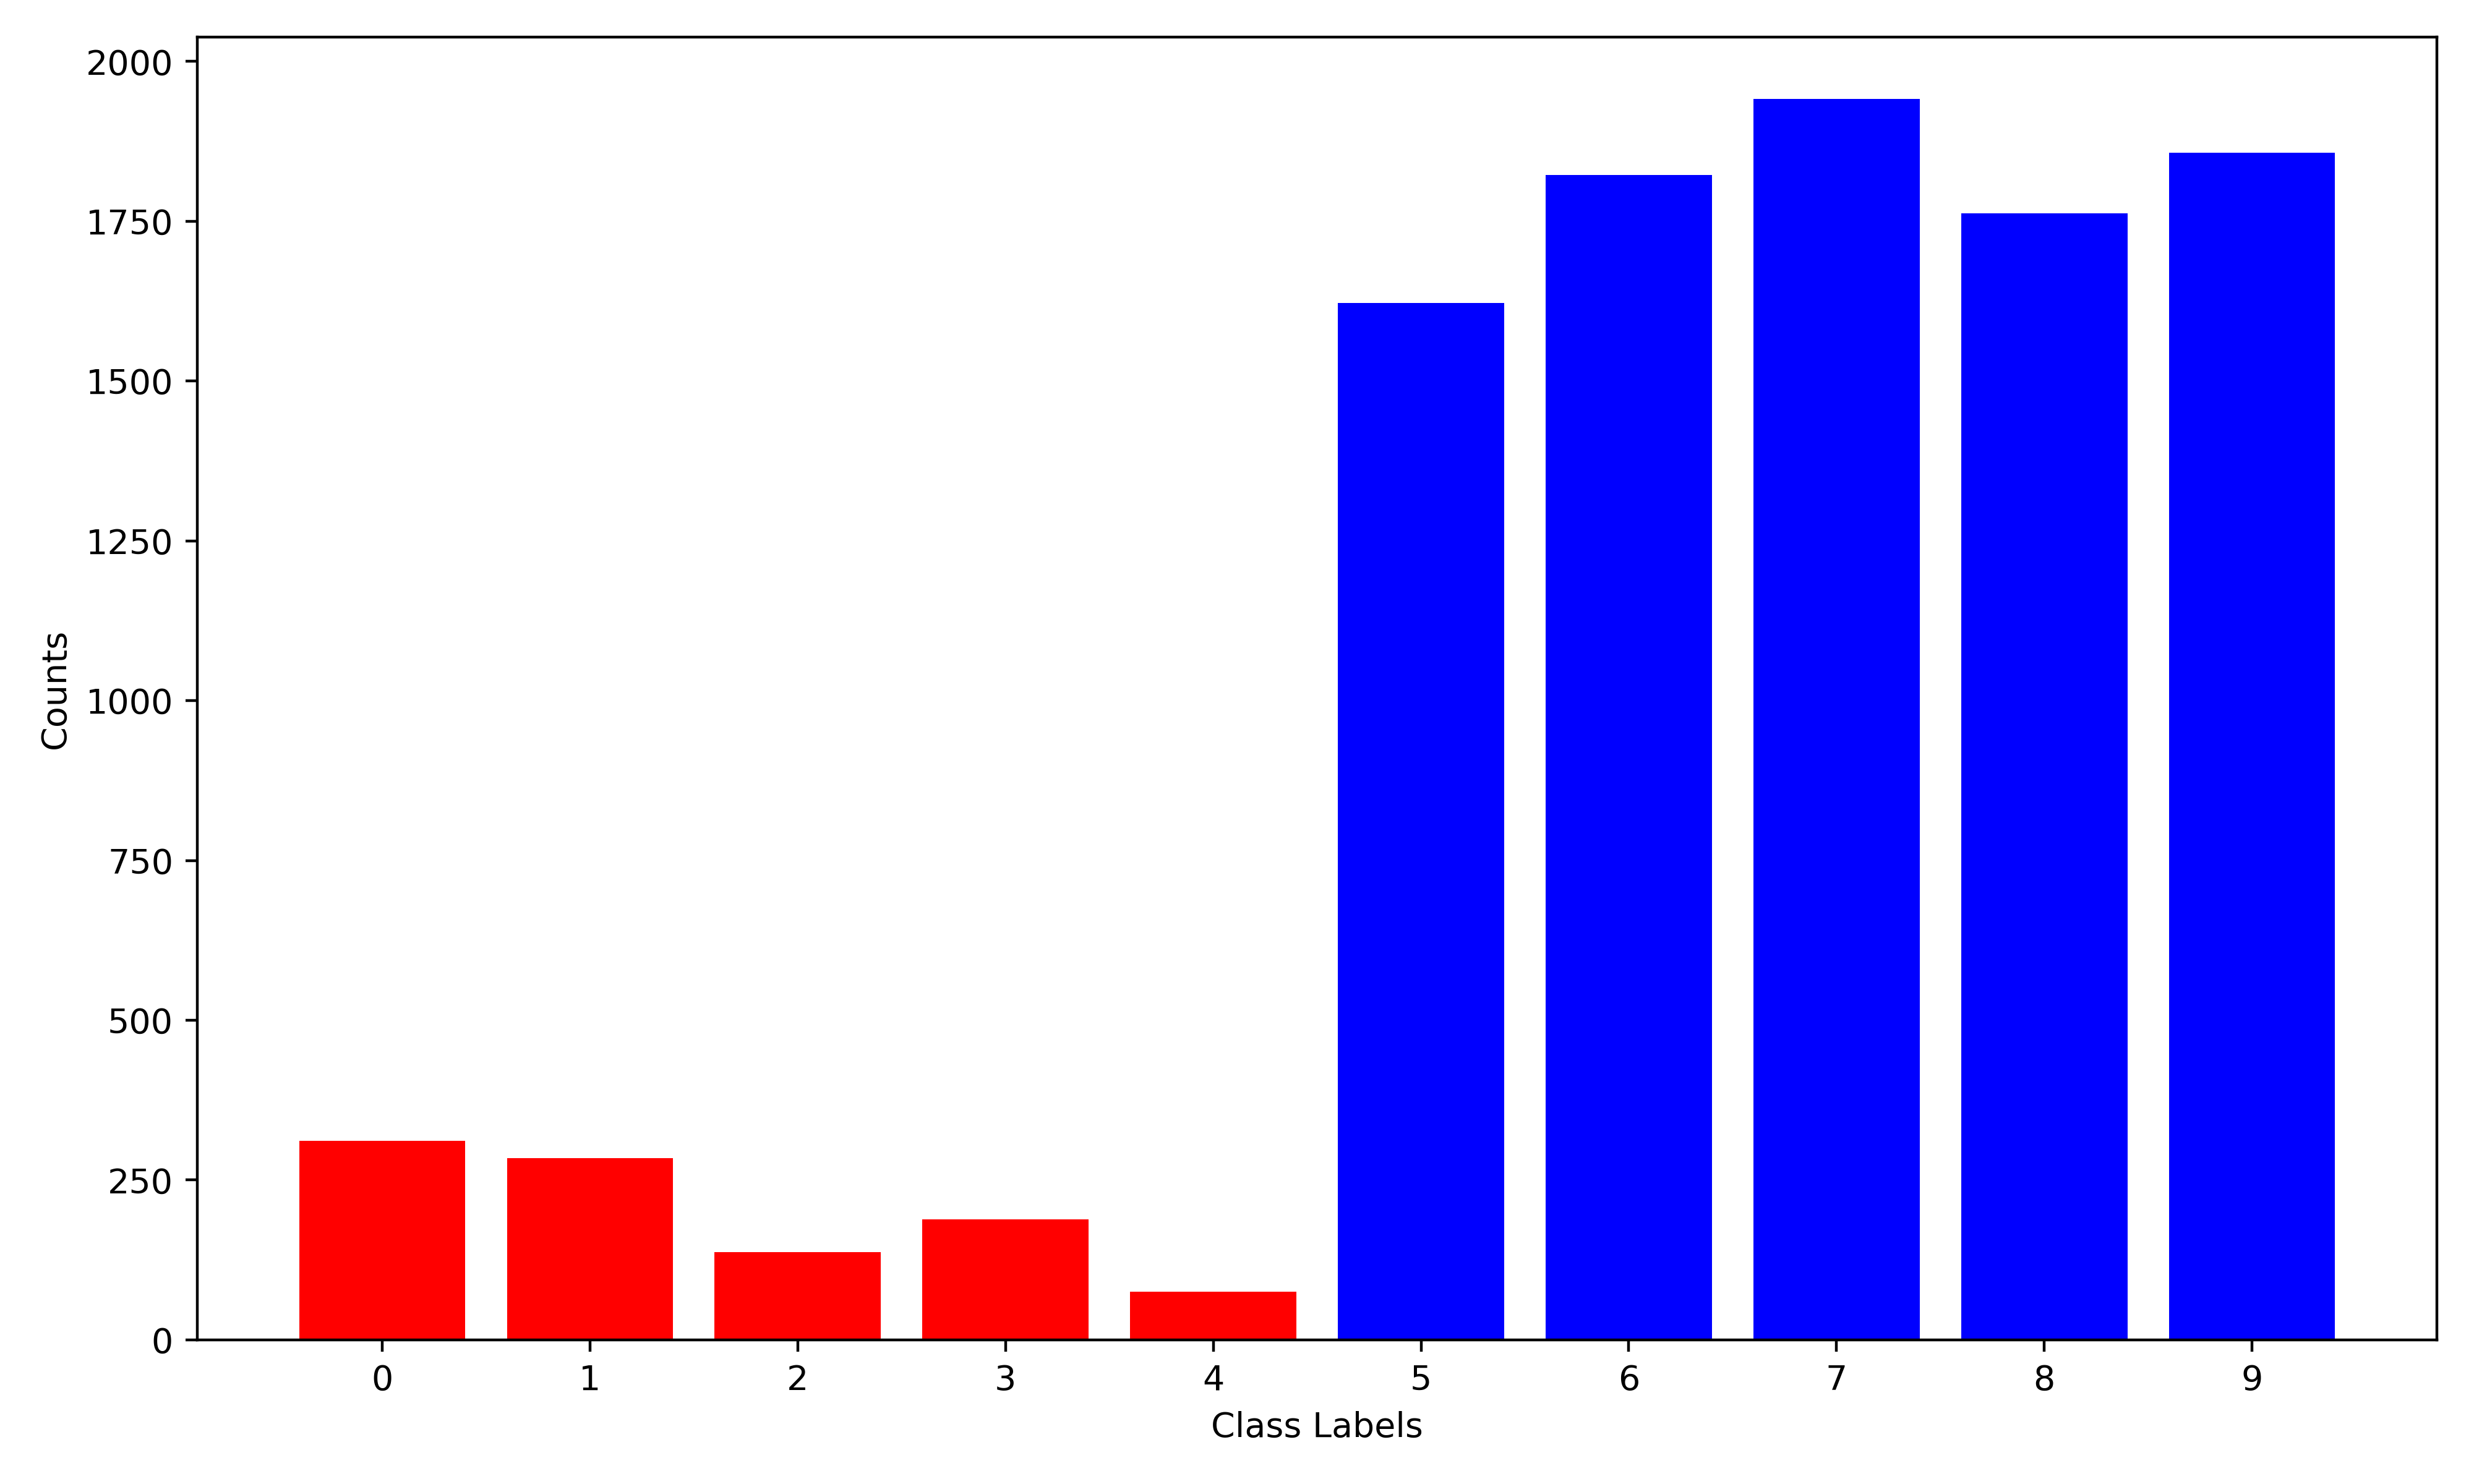
\includegraphics[width=0.8\textwidth]{Figures/Methods/dis_ub09.png}
    \end{subfigure}
    \hfill
    \begin{subfigure}{0.45\textwidth}
        \centering
        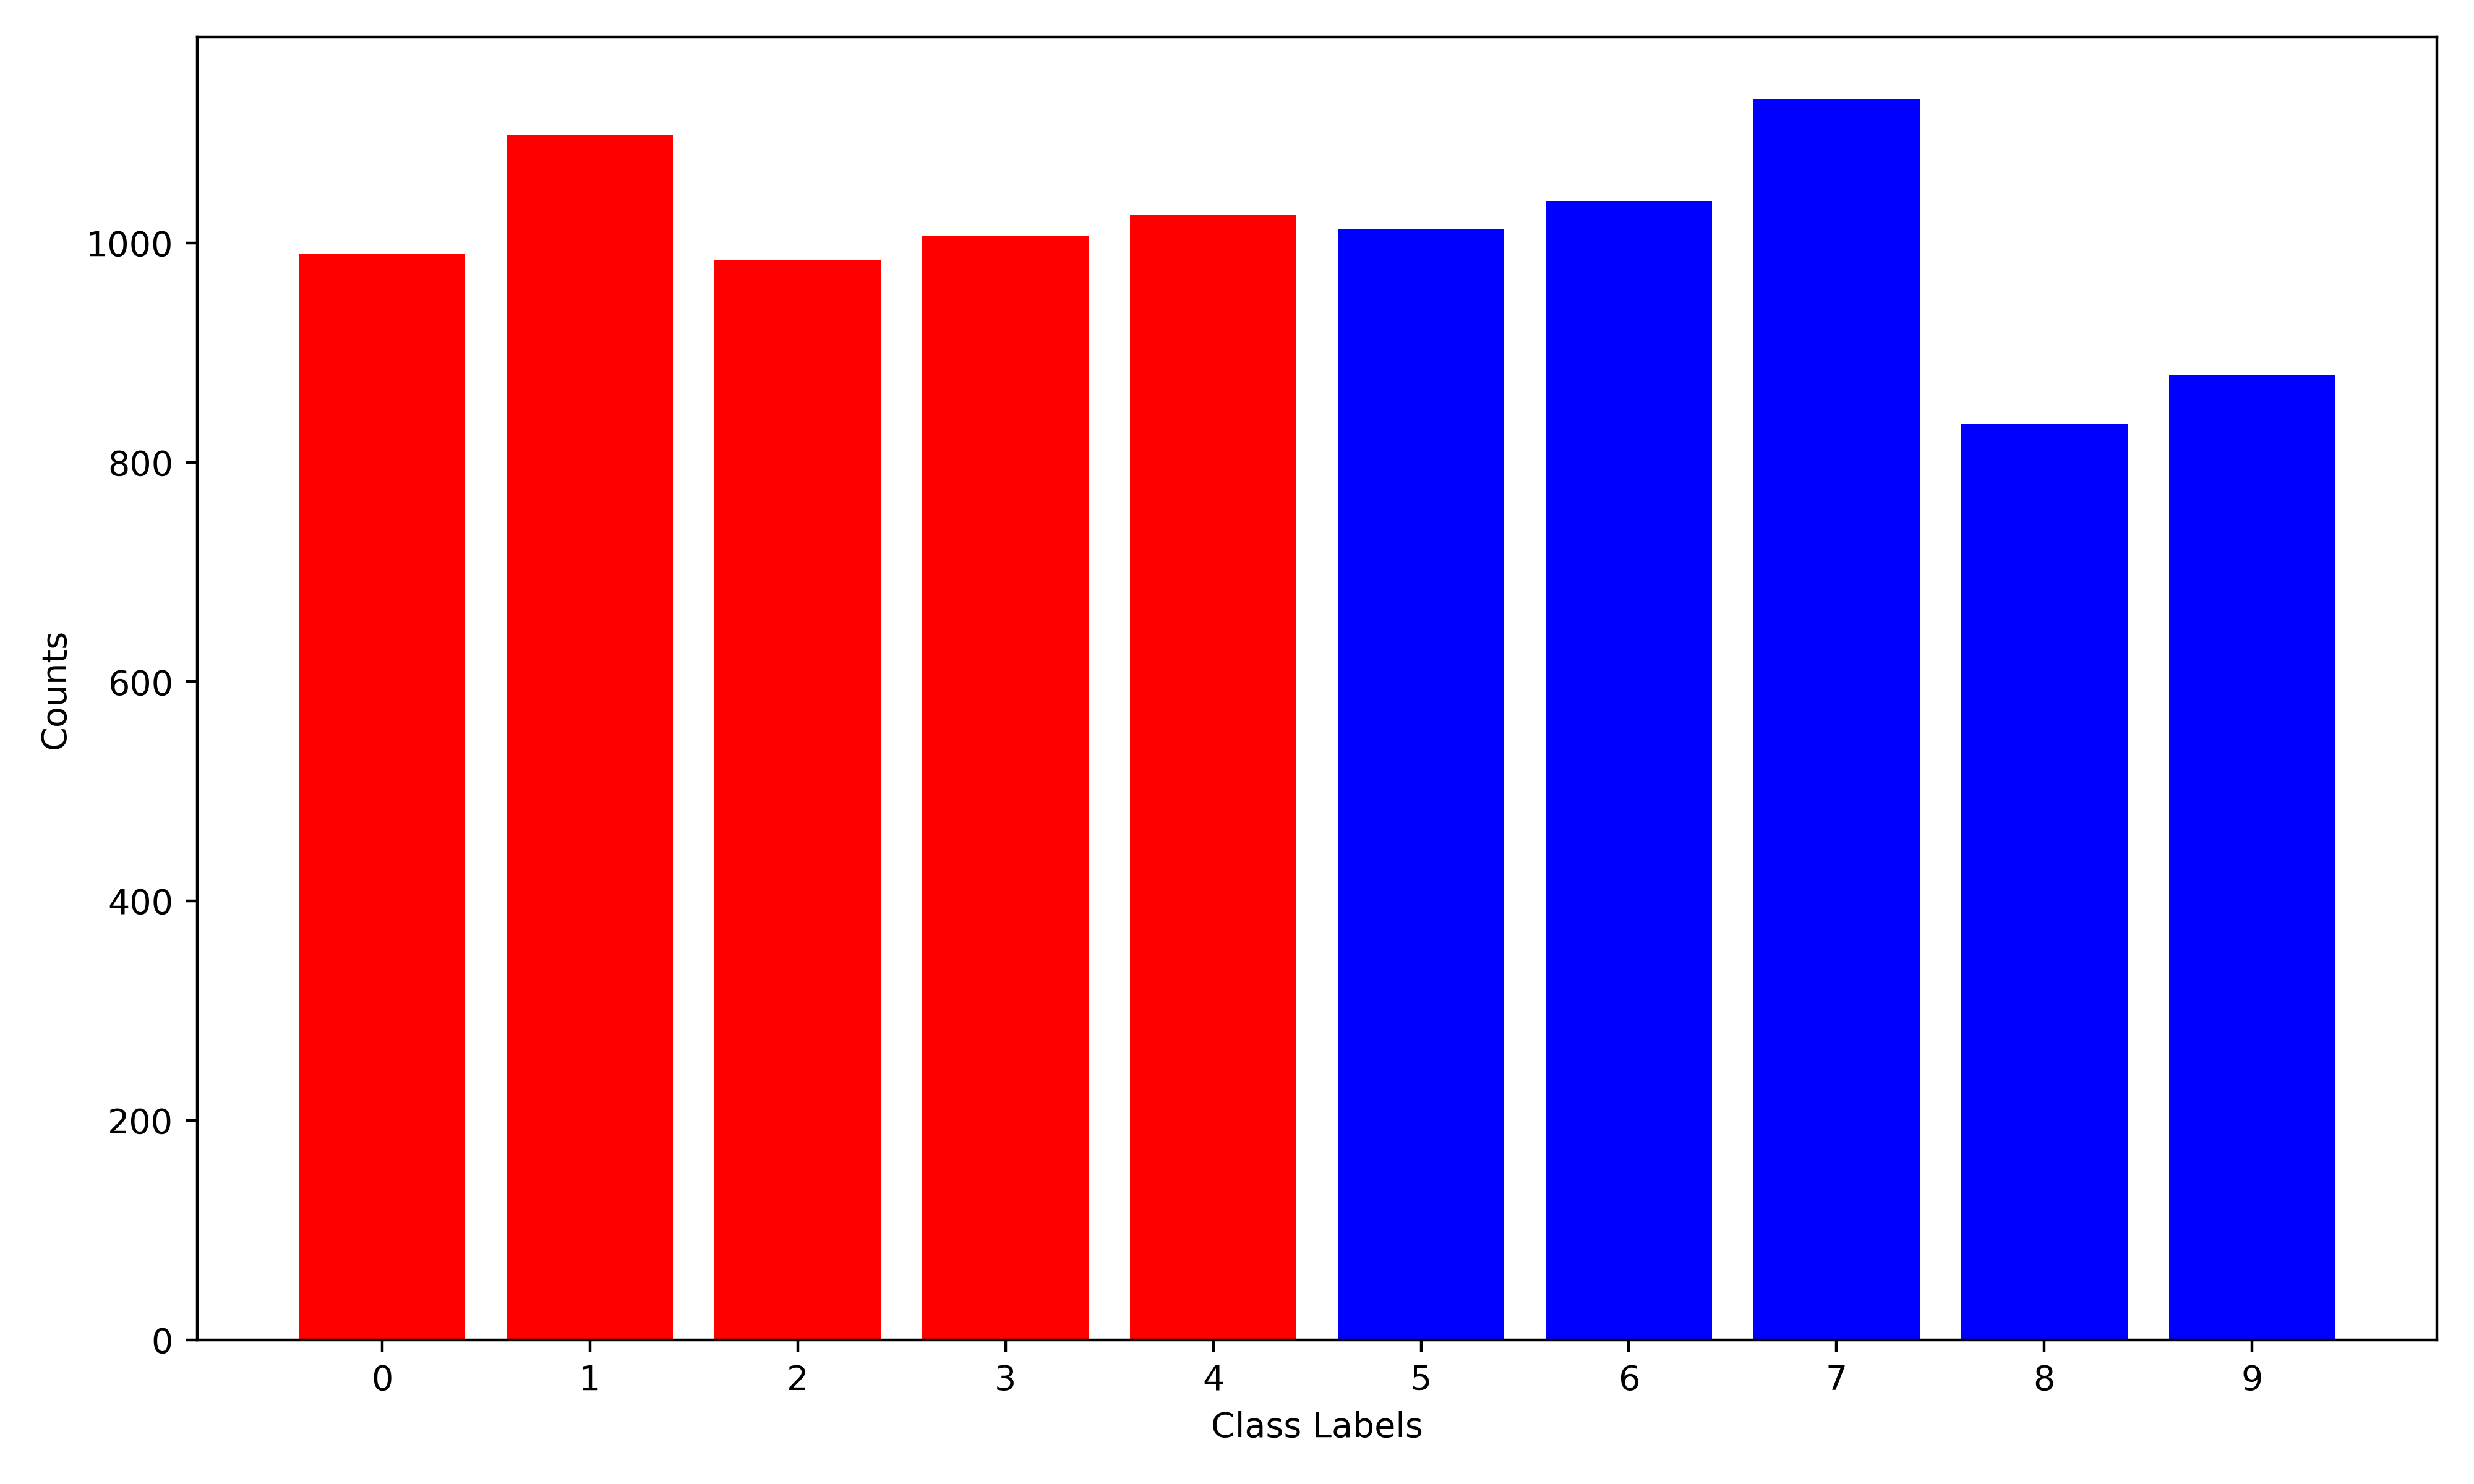
\includegraphics[width=0.8\textwidth]{Figures/Methods/dis_ub09_inw.png}
    \end{subfigure}
    \hfill
    \begin{subfigure}{0.45\textwidth}
        \centering
        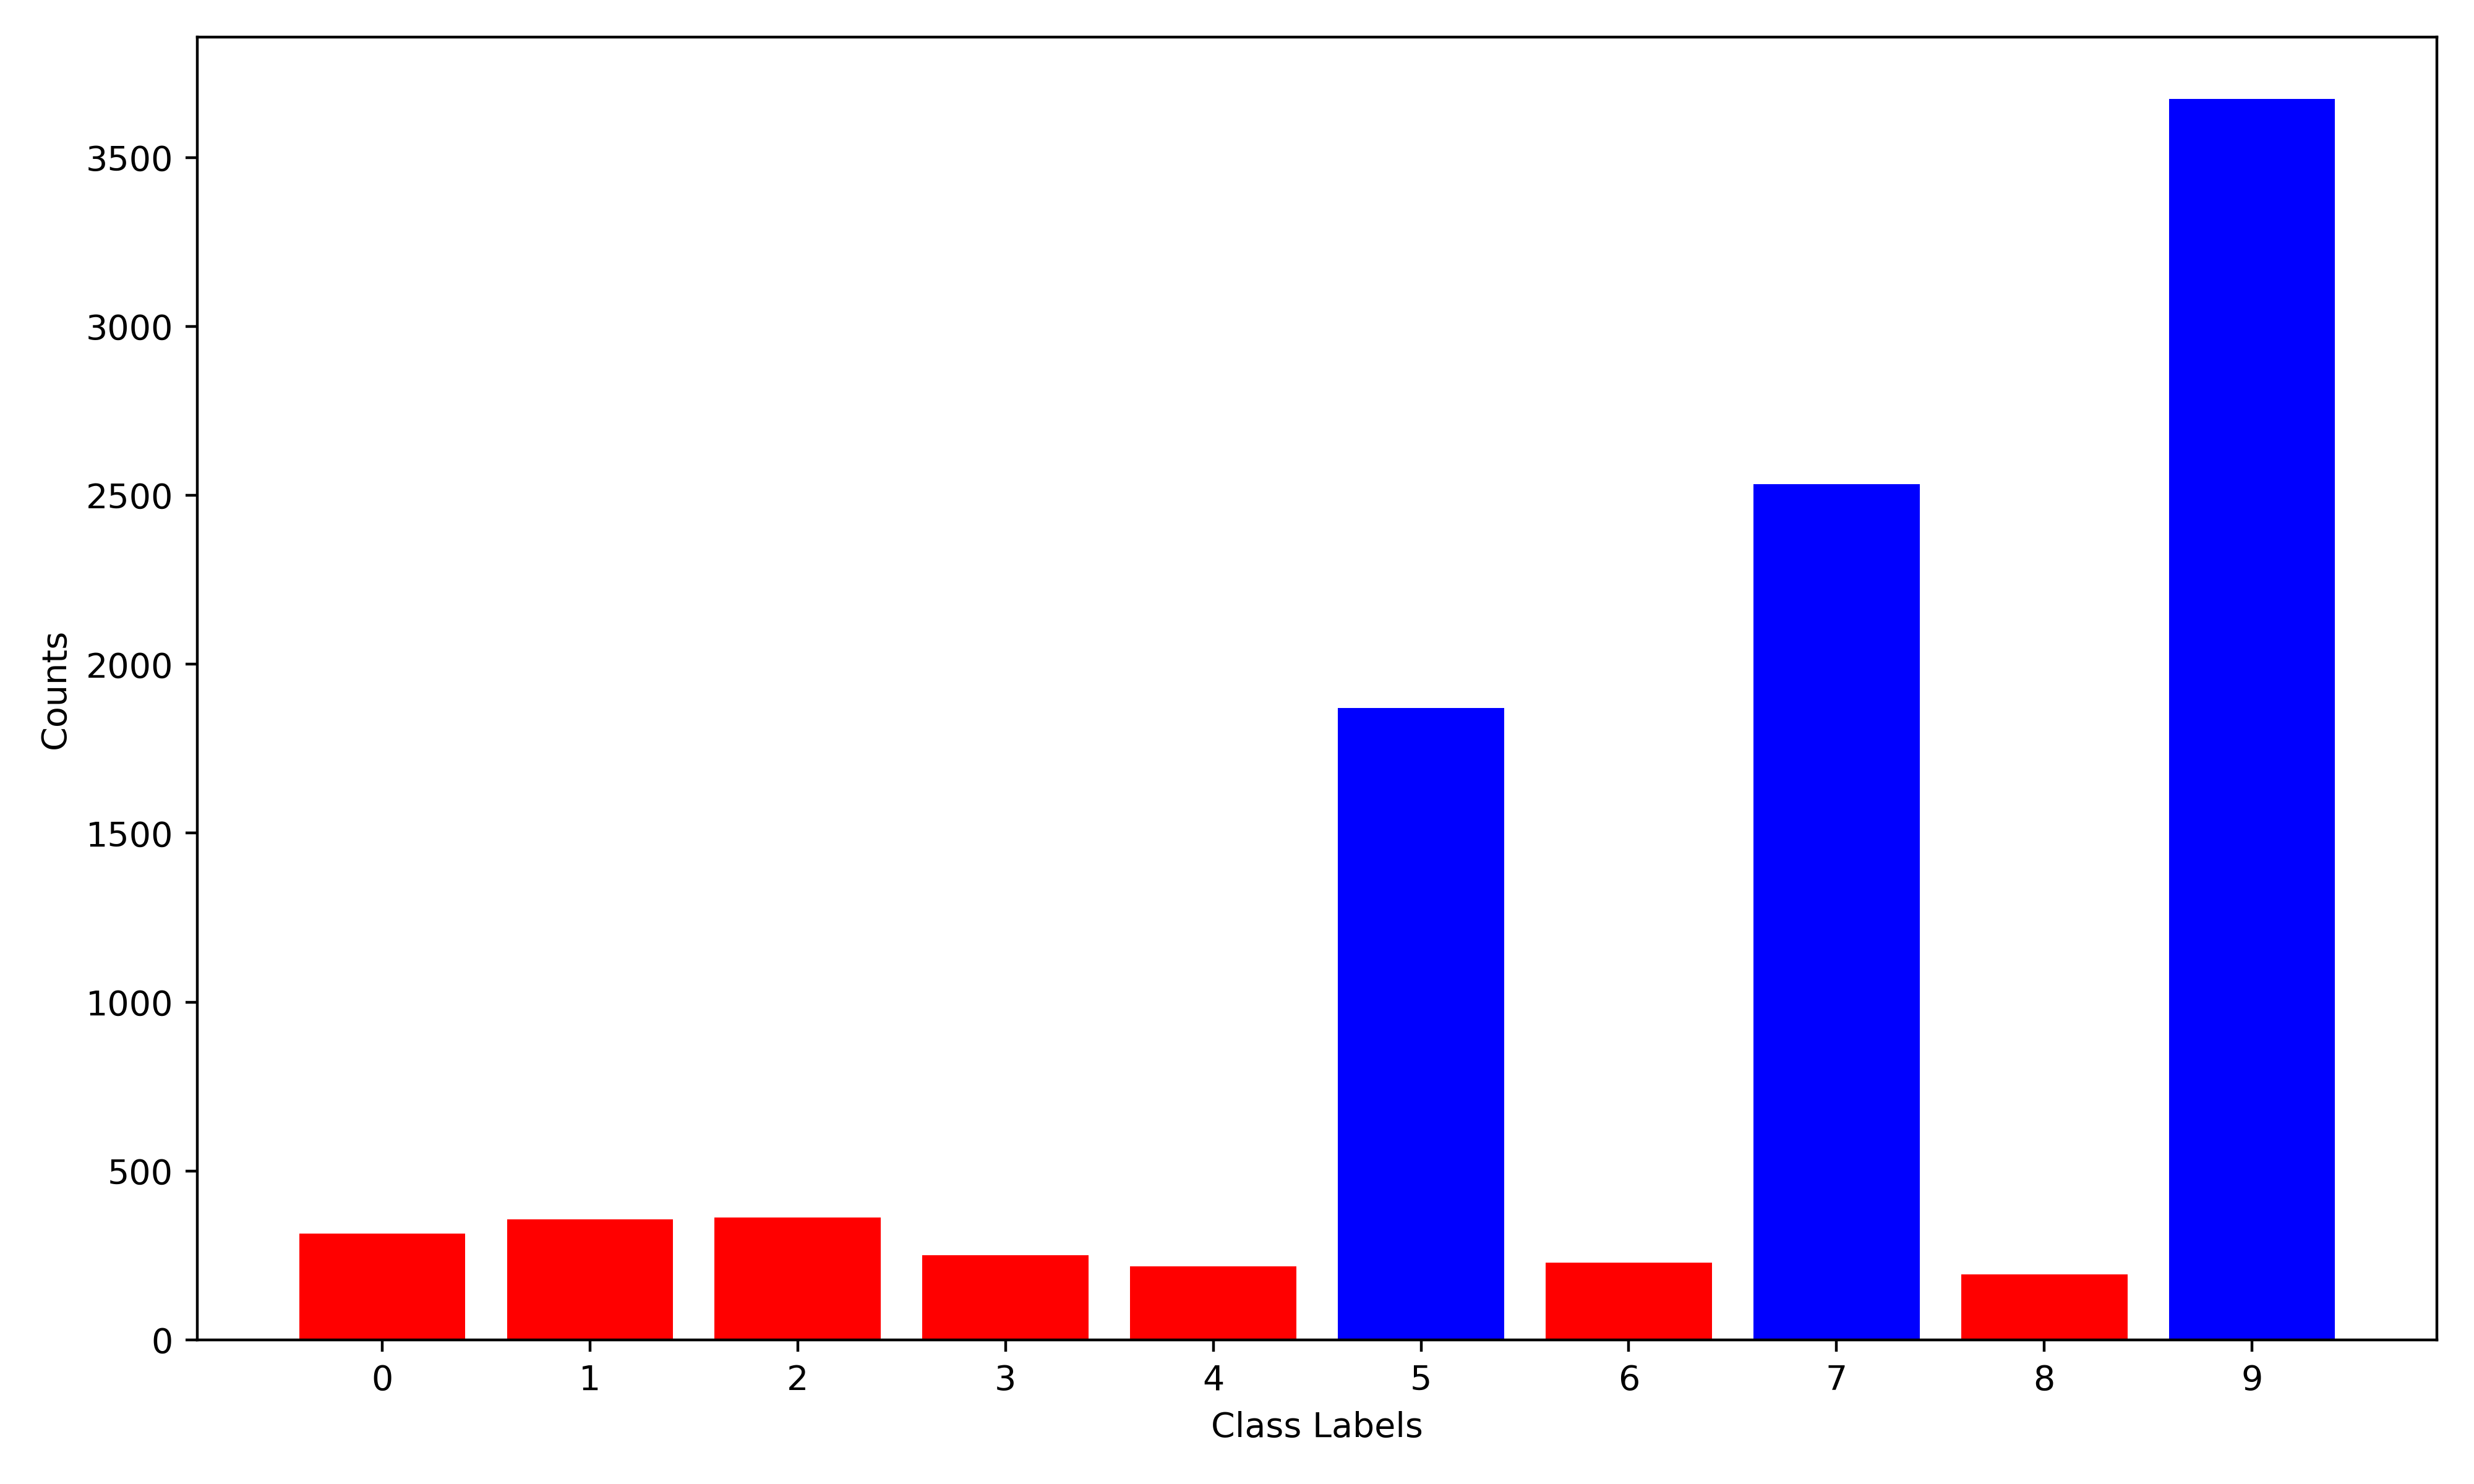
\includegraphics[width=0.8\textwidth]{Figures/Methods/dis_ubfs.png}
    \end{subfigure}
    \hfill
    \begin{subfigure}{0.45\textwidth}
        \centering
        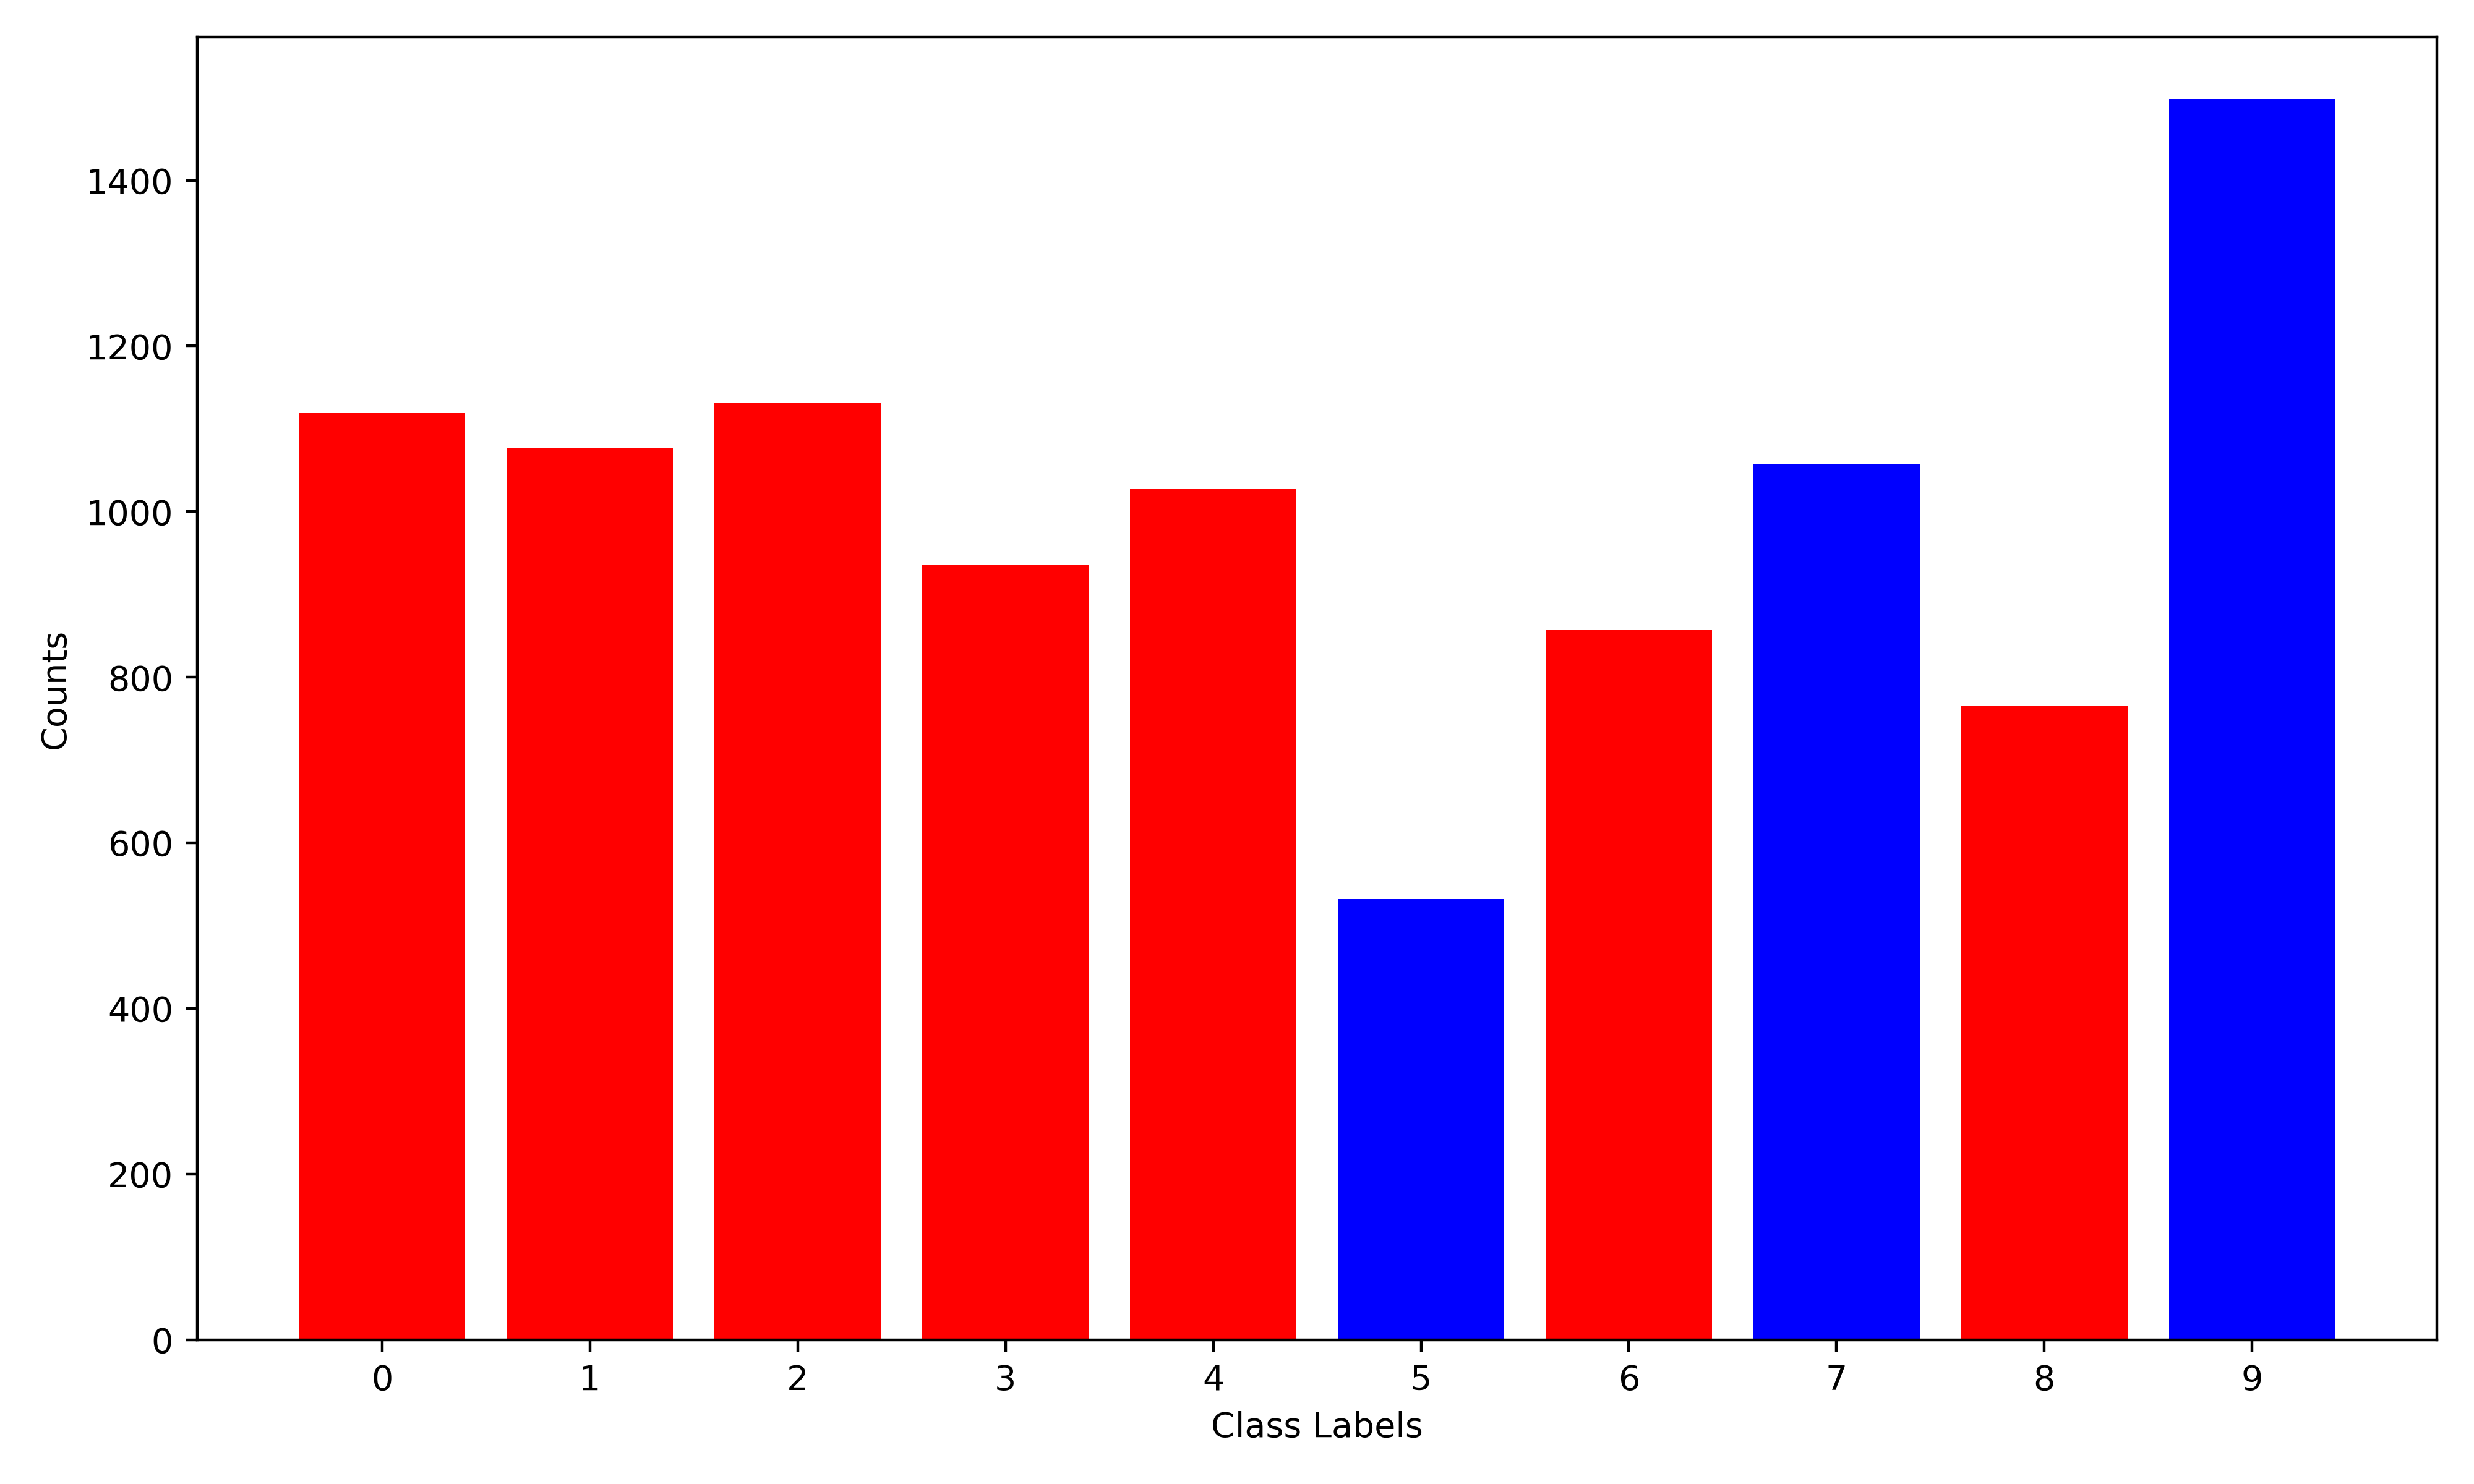
\includegraphics[width=0.8\textwidth]{Figures/Methods/dis_ubfs_inw.png}
    \end{subfigure}
    \caption{Number of generated samples in each class for the unbalanced MNIST dataset: Vanilla Gen-RKM (top left) vs. Gen-RKM with inverse frequency sampling (top right). For the Fashion MNIST dataset: Vanilla Gen-RKM (down left) vs. Gen-RKM with inverse frequency sampling (down right). A rebalancing effect is visible}
    \label{dis-ub09}
\end{figure}



\begin{figure}[H]
    \centering
    \begin{subfigure}{0.45\textwidth}
        \centering
        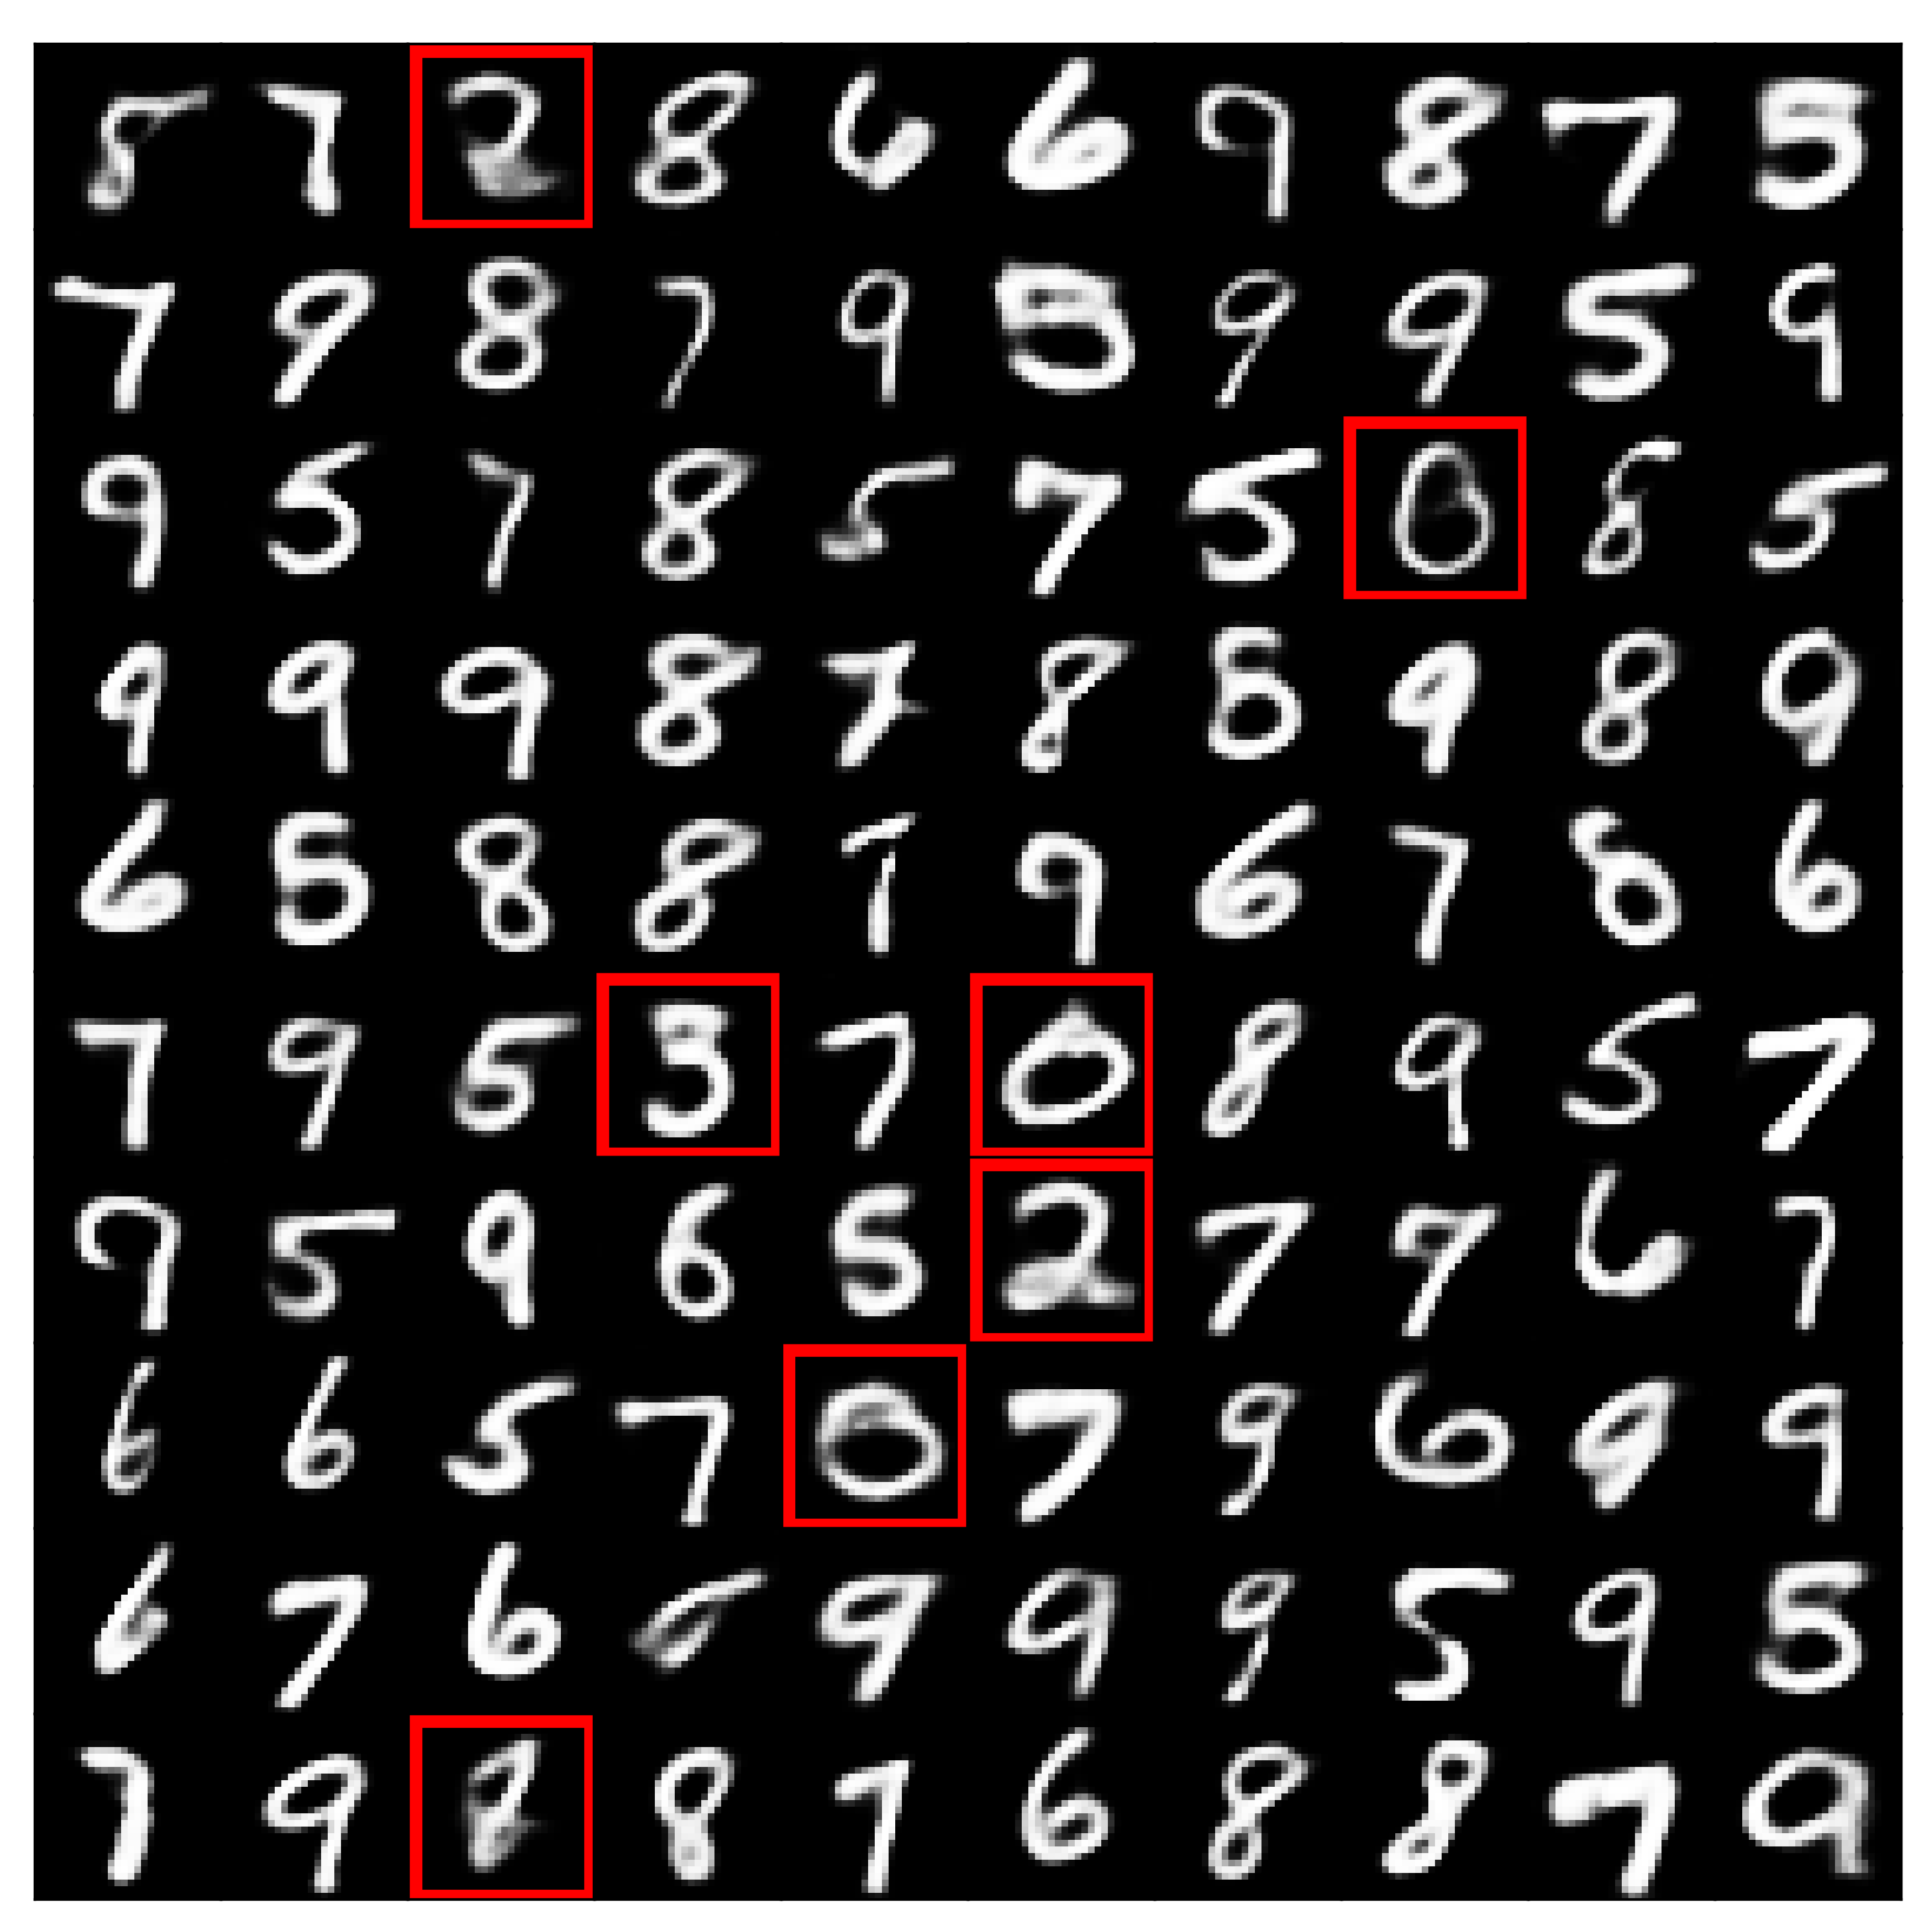
\includegraphics[width=0.7\textwidth]{Figures/Methods/ub09_random_generation.png}
    \end{subfigure}
    \hfill
    \begin{subfigure}{0.45\textwidth}
        \centering
        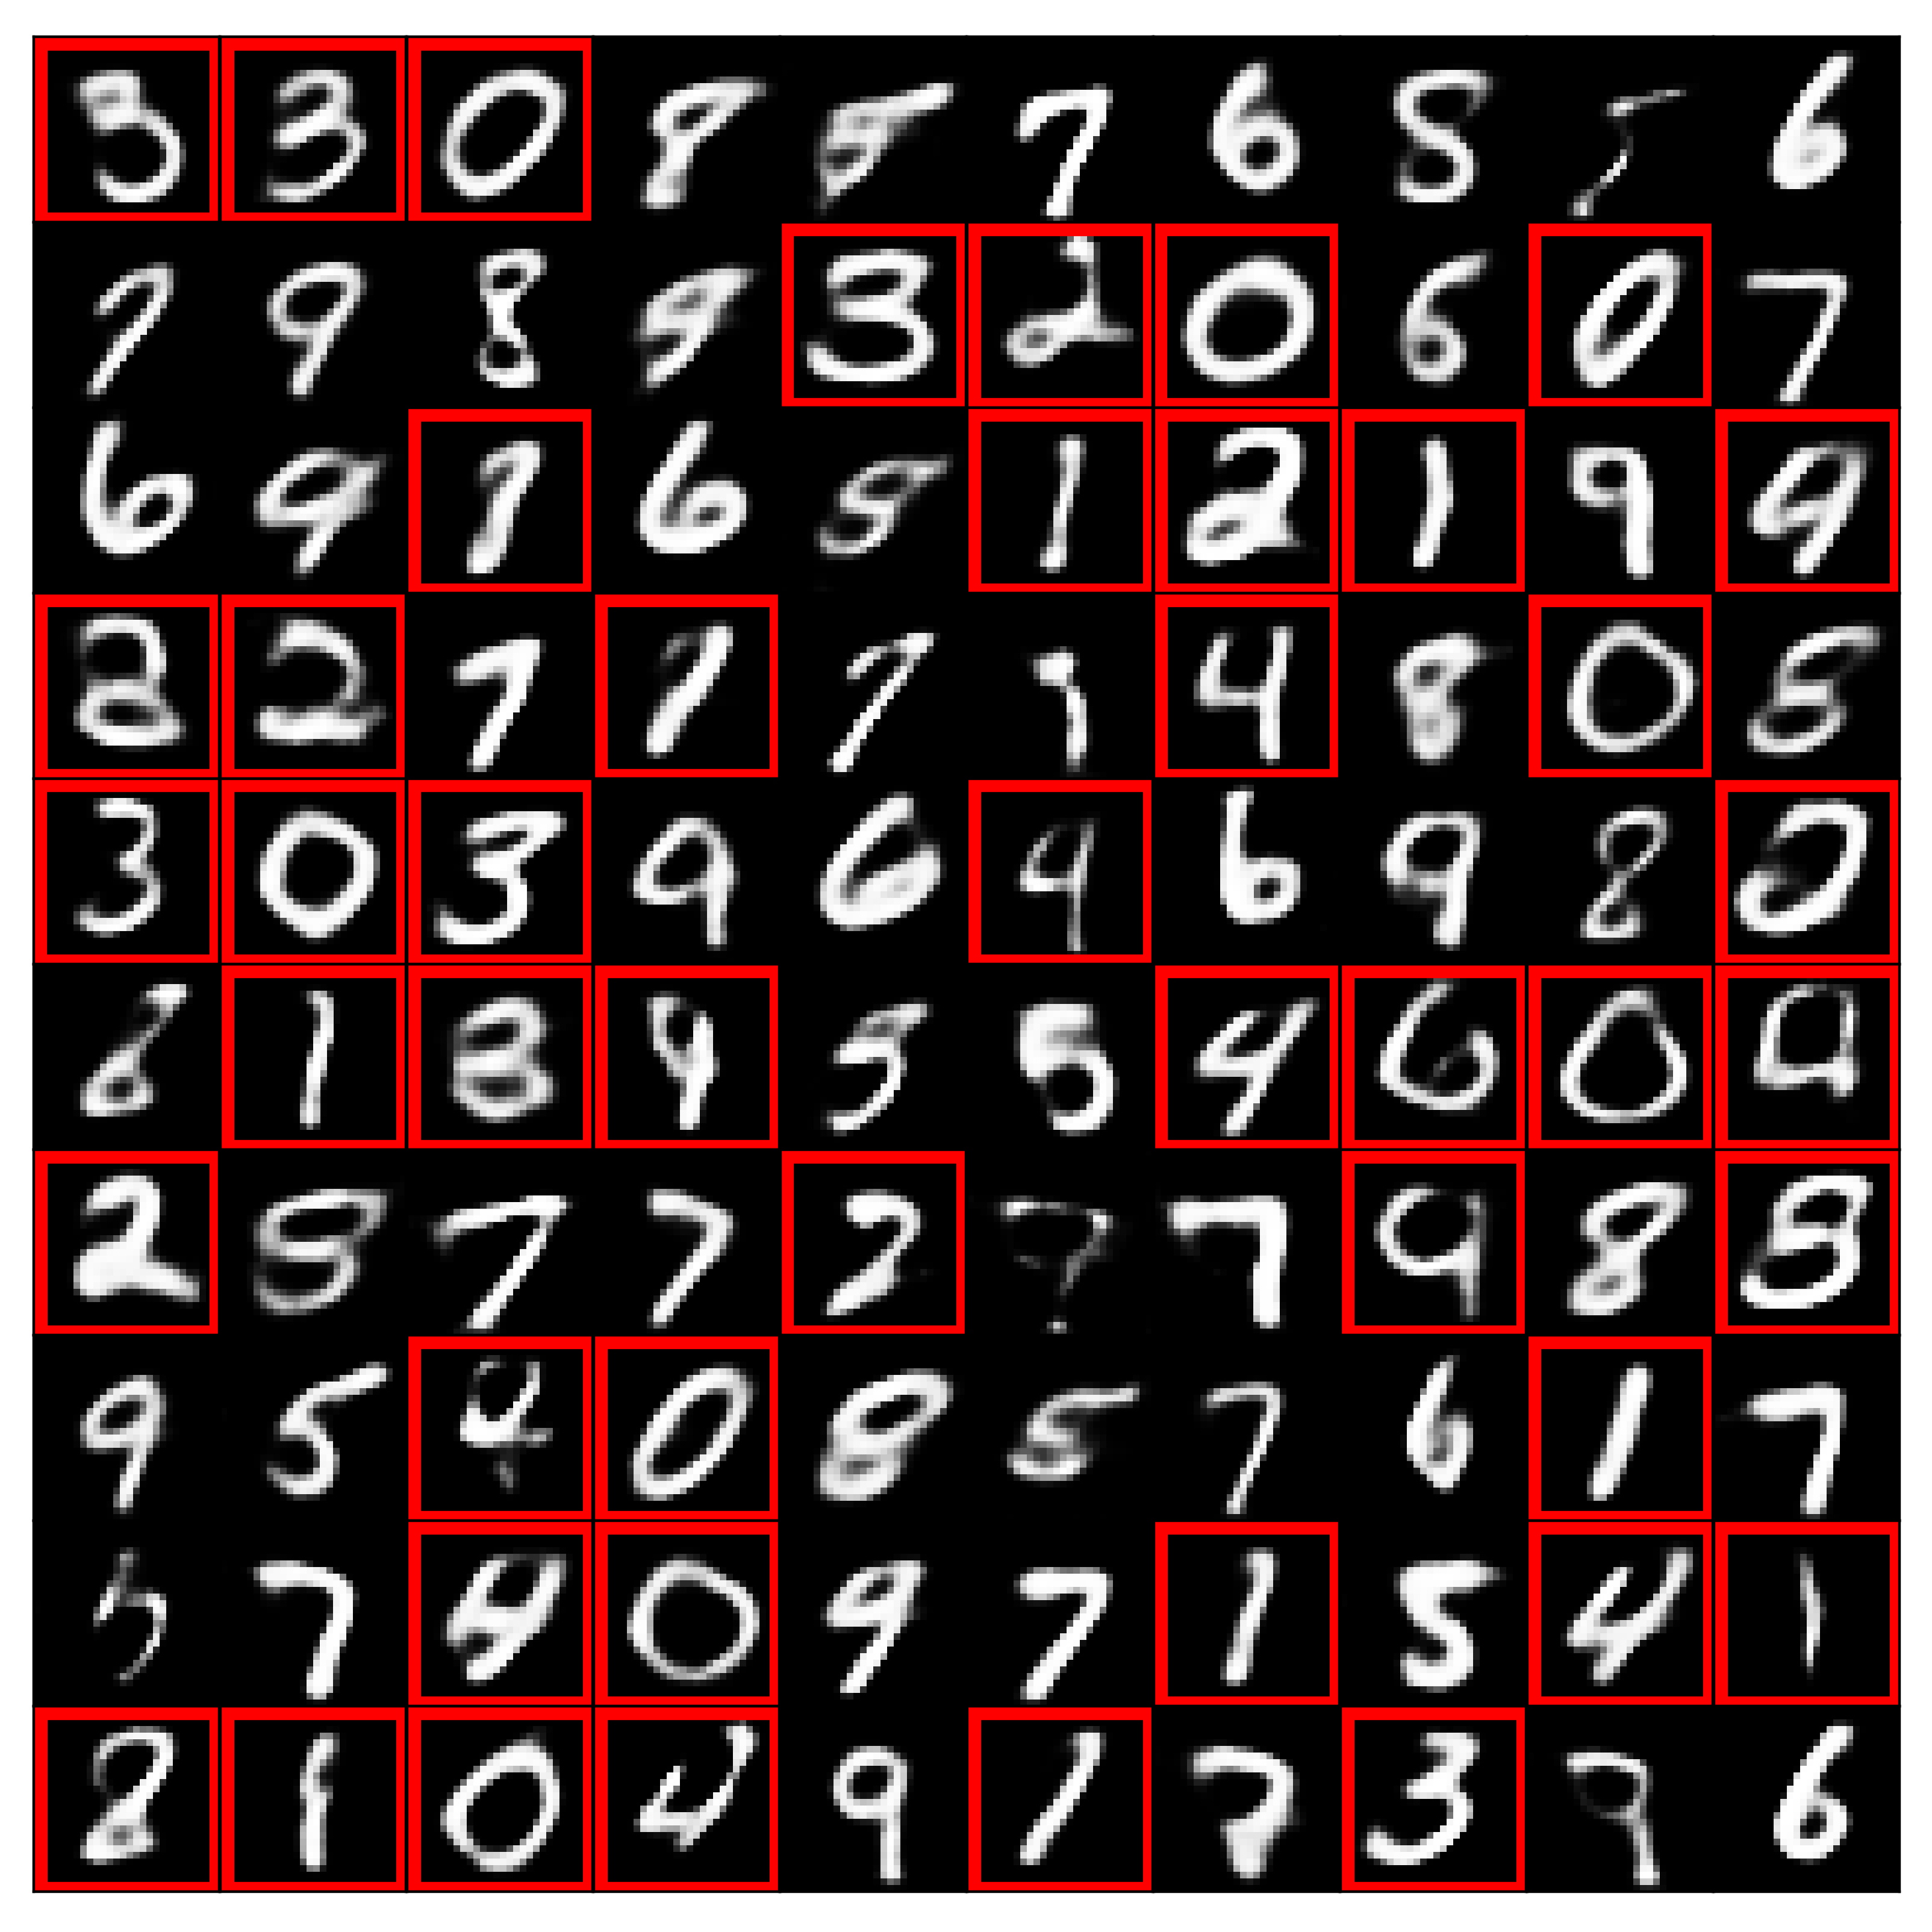
\includegraphics[width=0.7\textwidth]{Figures/Methods/invw_ub09_random_generation.png}
    \end{subfigure}
    \hfill
    \begin{subfigure}{0.45\textwidth}
        \centering
        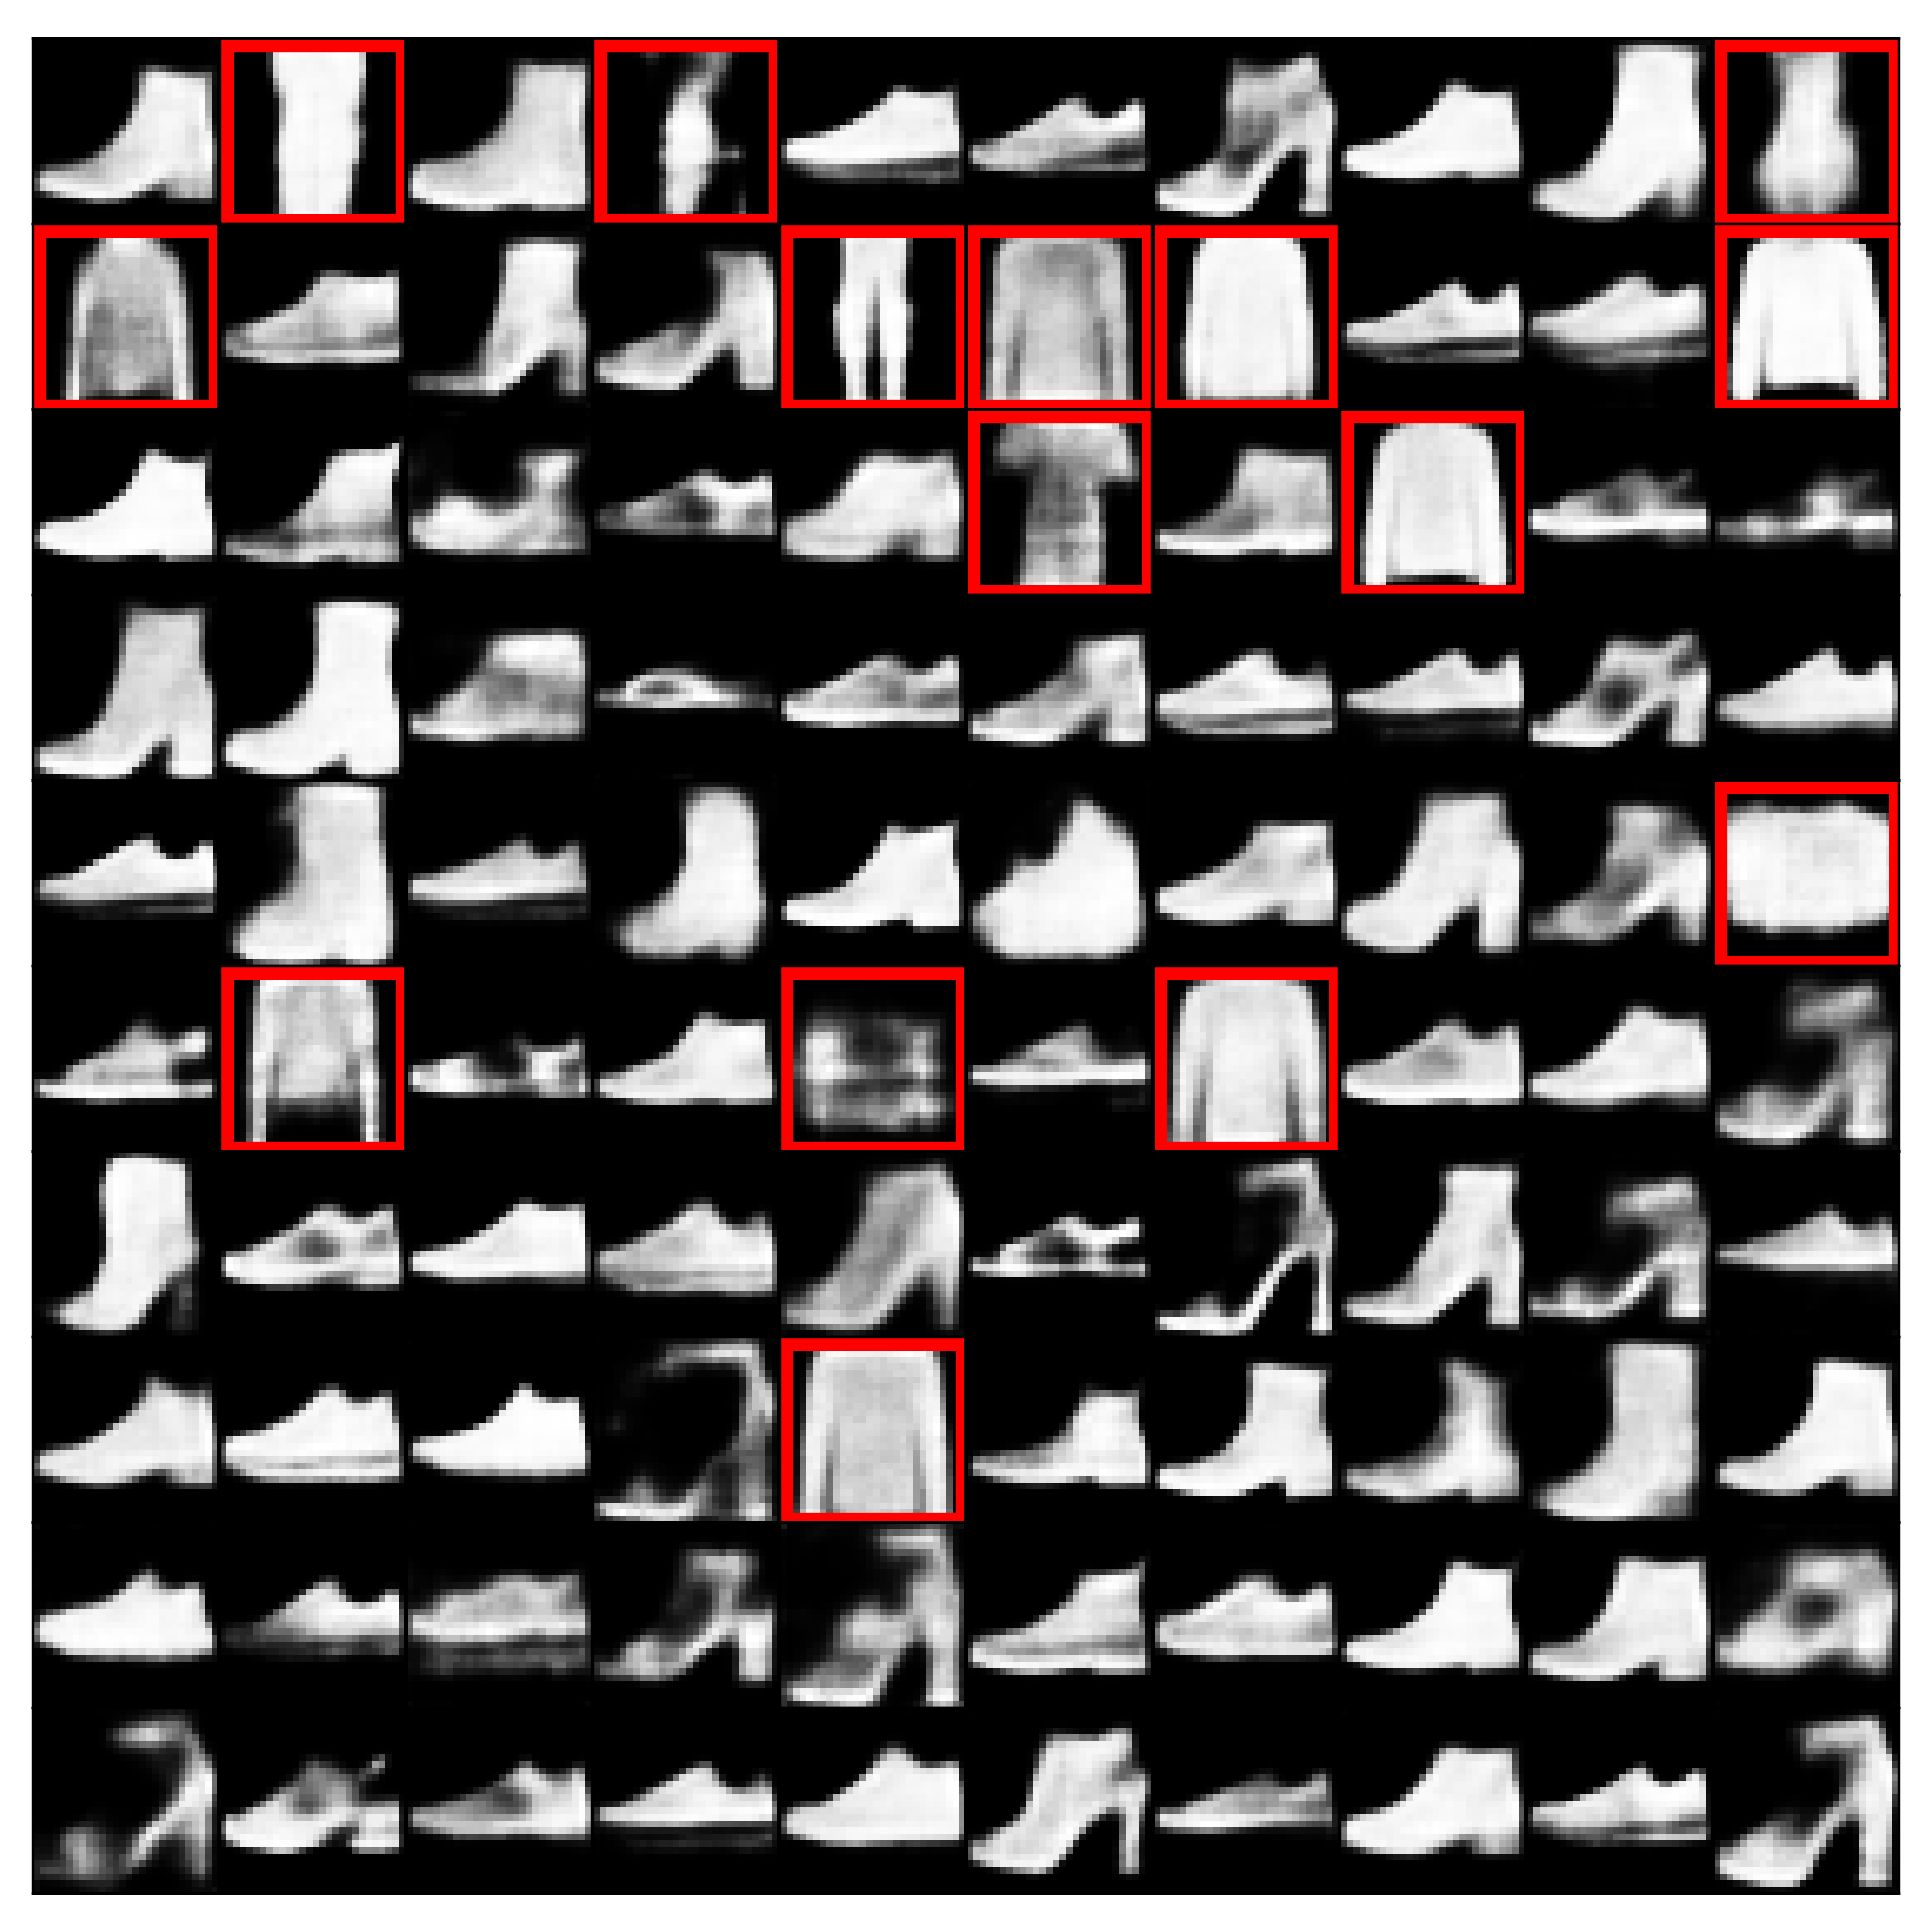
\includegraphics[width=0.7\textwidth]{Figures/Methods/FSM_random_generation.png}
    \end{subfigure}
    \hfill
    \begin{subfigure}{0.45\textwidth}
        \centering
        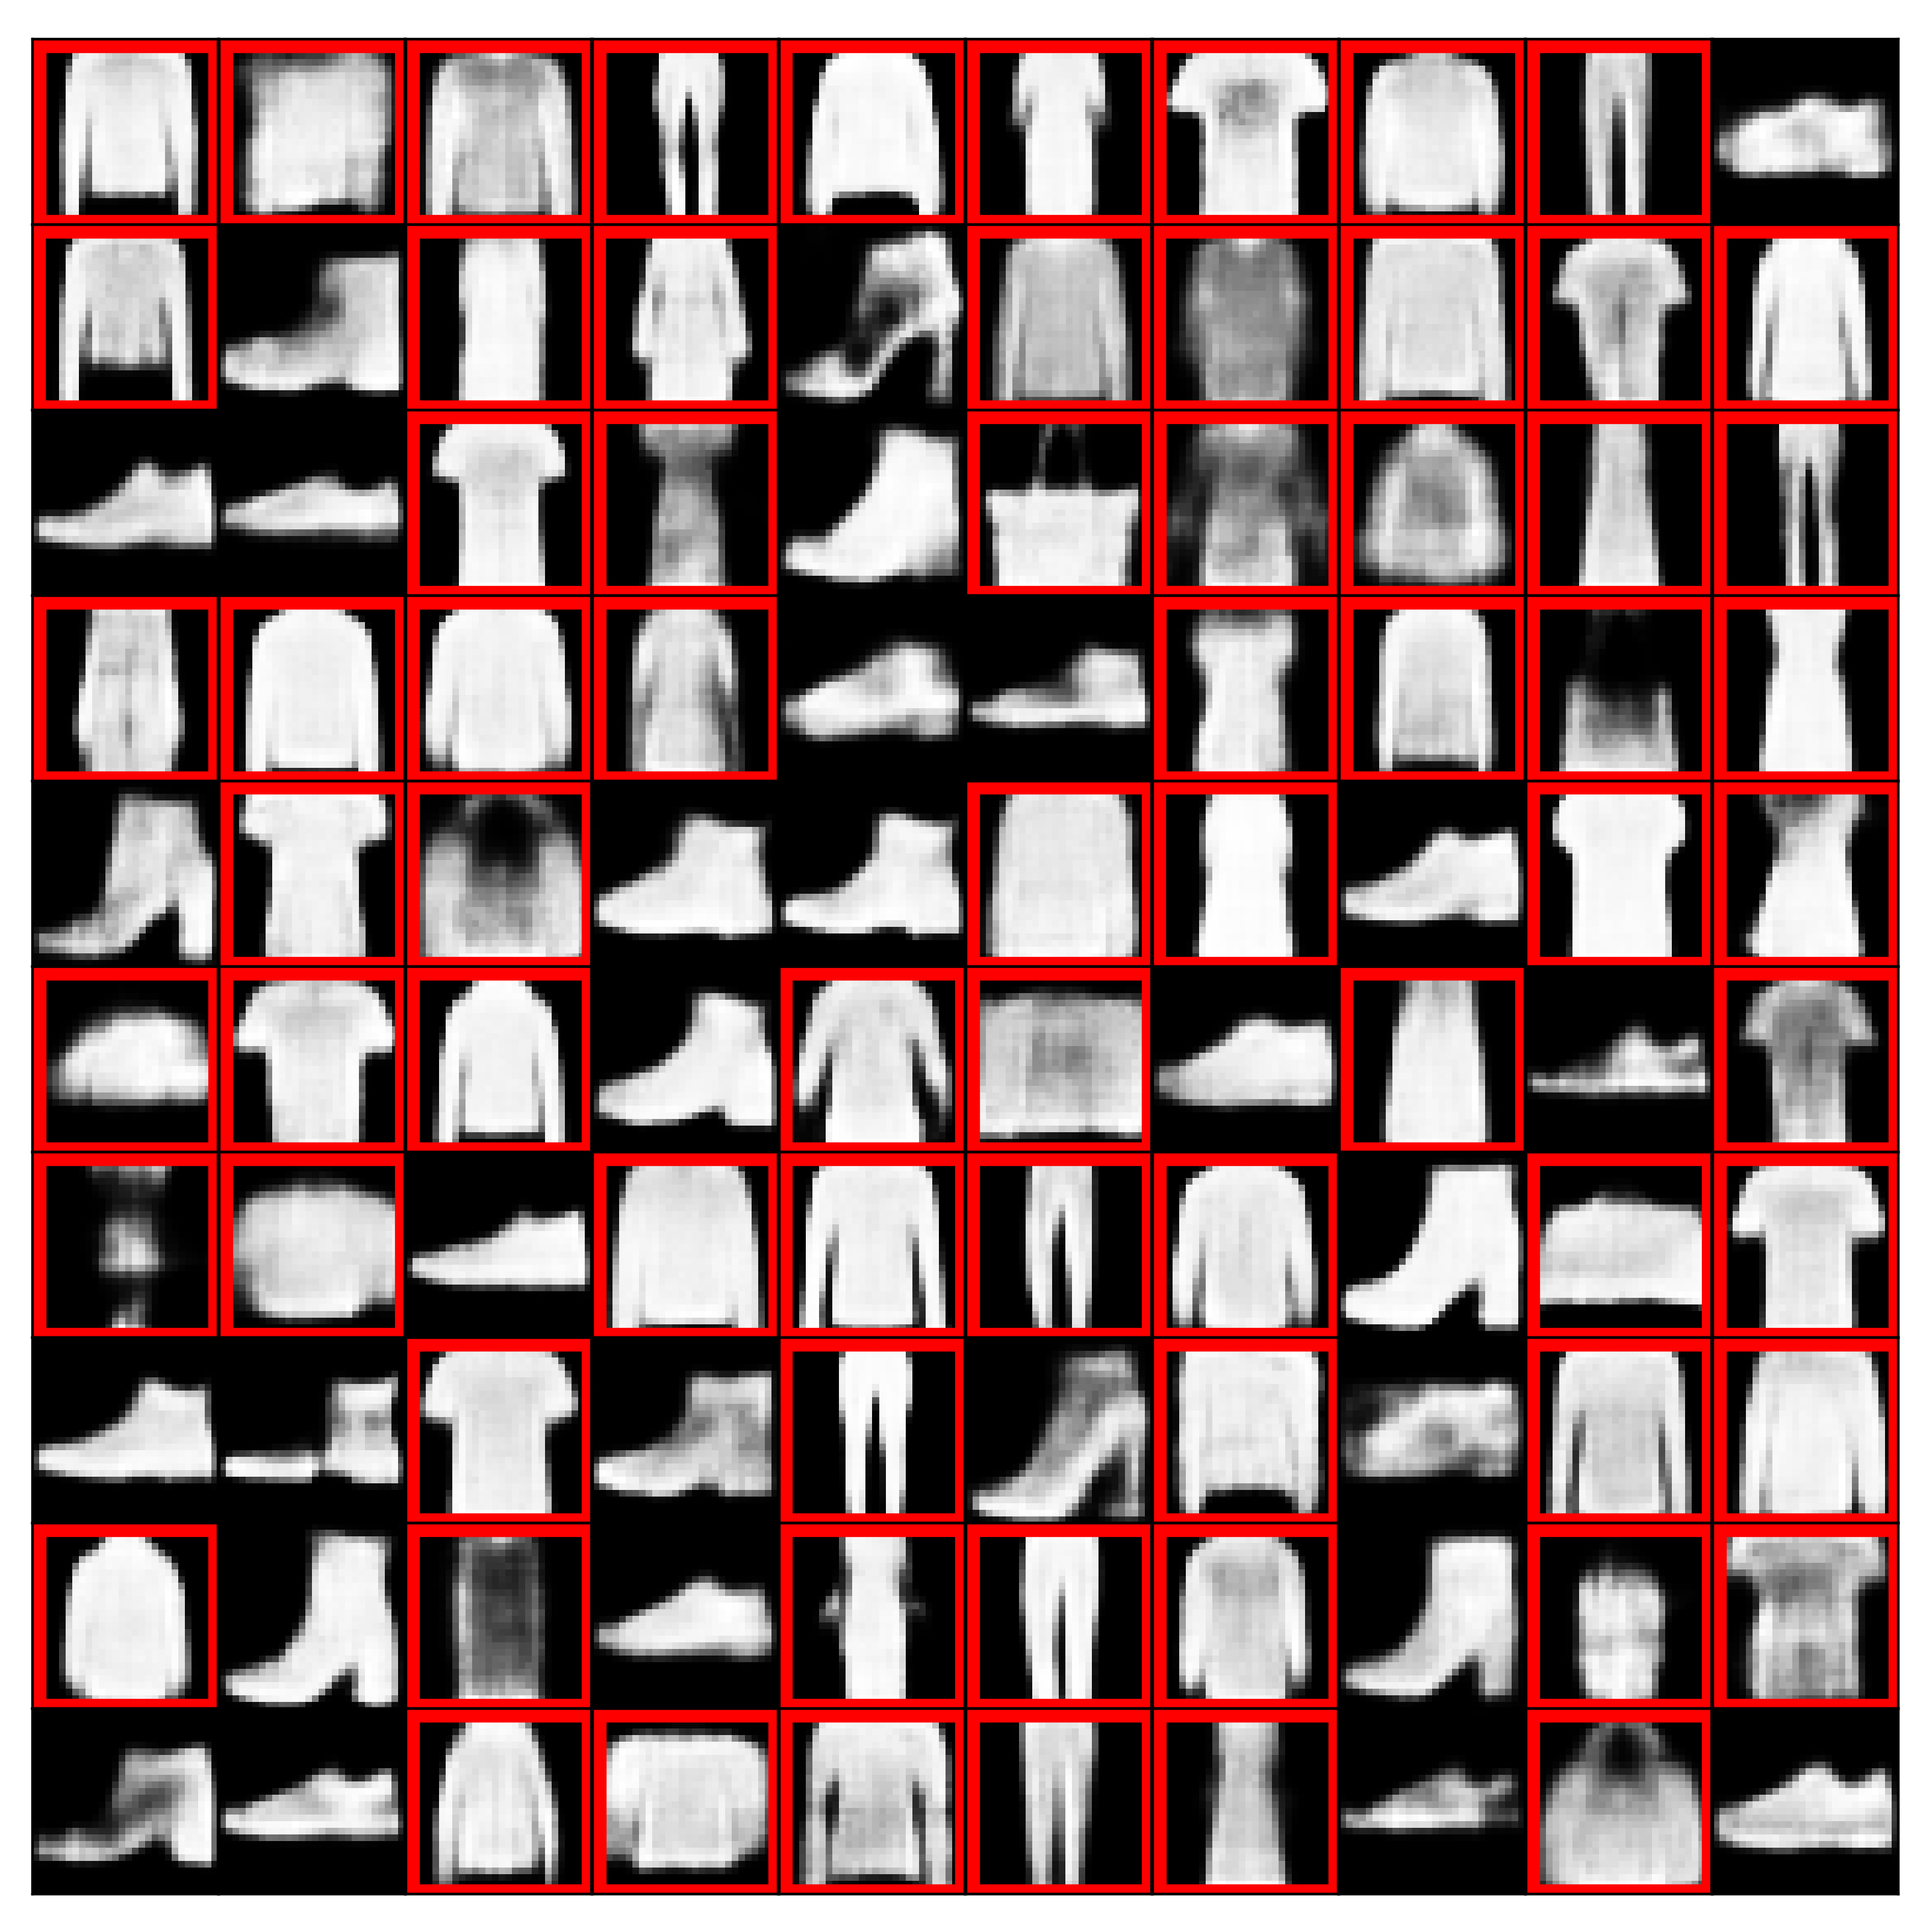
\includegraphics[width=0.7\textwidth]{Figures/Methods/FSM_invw_random_generation.png}
    \end{subfigure}
    \caption{Random generation of unbalanced MNIST dataset: vanilla Gen-RKM (top right) and Gen-RKM with inverse frequency sampling (top left). Fashion MNIST dataset: vanilla Gen-RKM (down right) and Gen-RKM with inverse frequency sampling (down left)}
    \label{fig-ub09}
\end{figure}


% \begin{figure}[H]
%     \centering
%     \begin{subfigure}{0.45\textwidth}
%         \centering
%         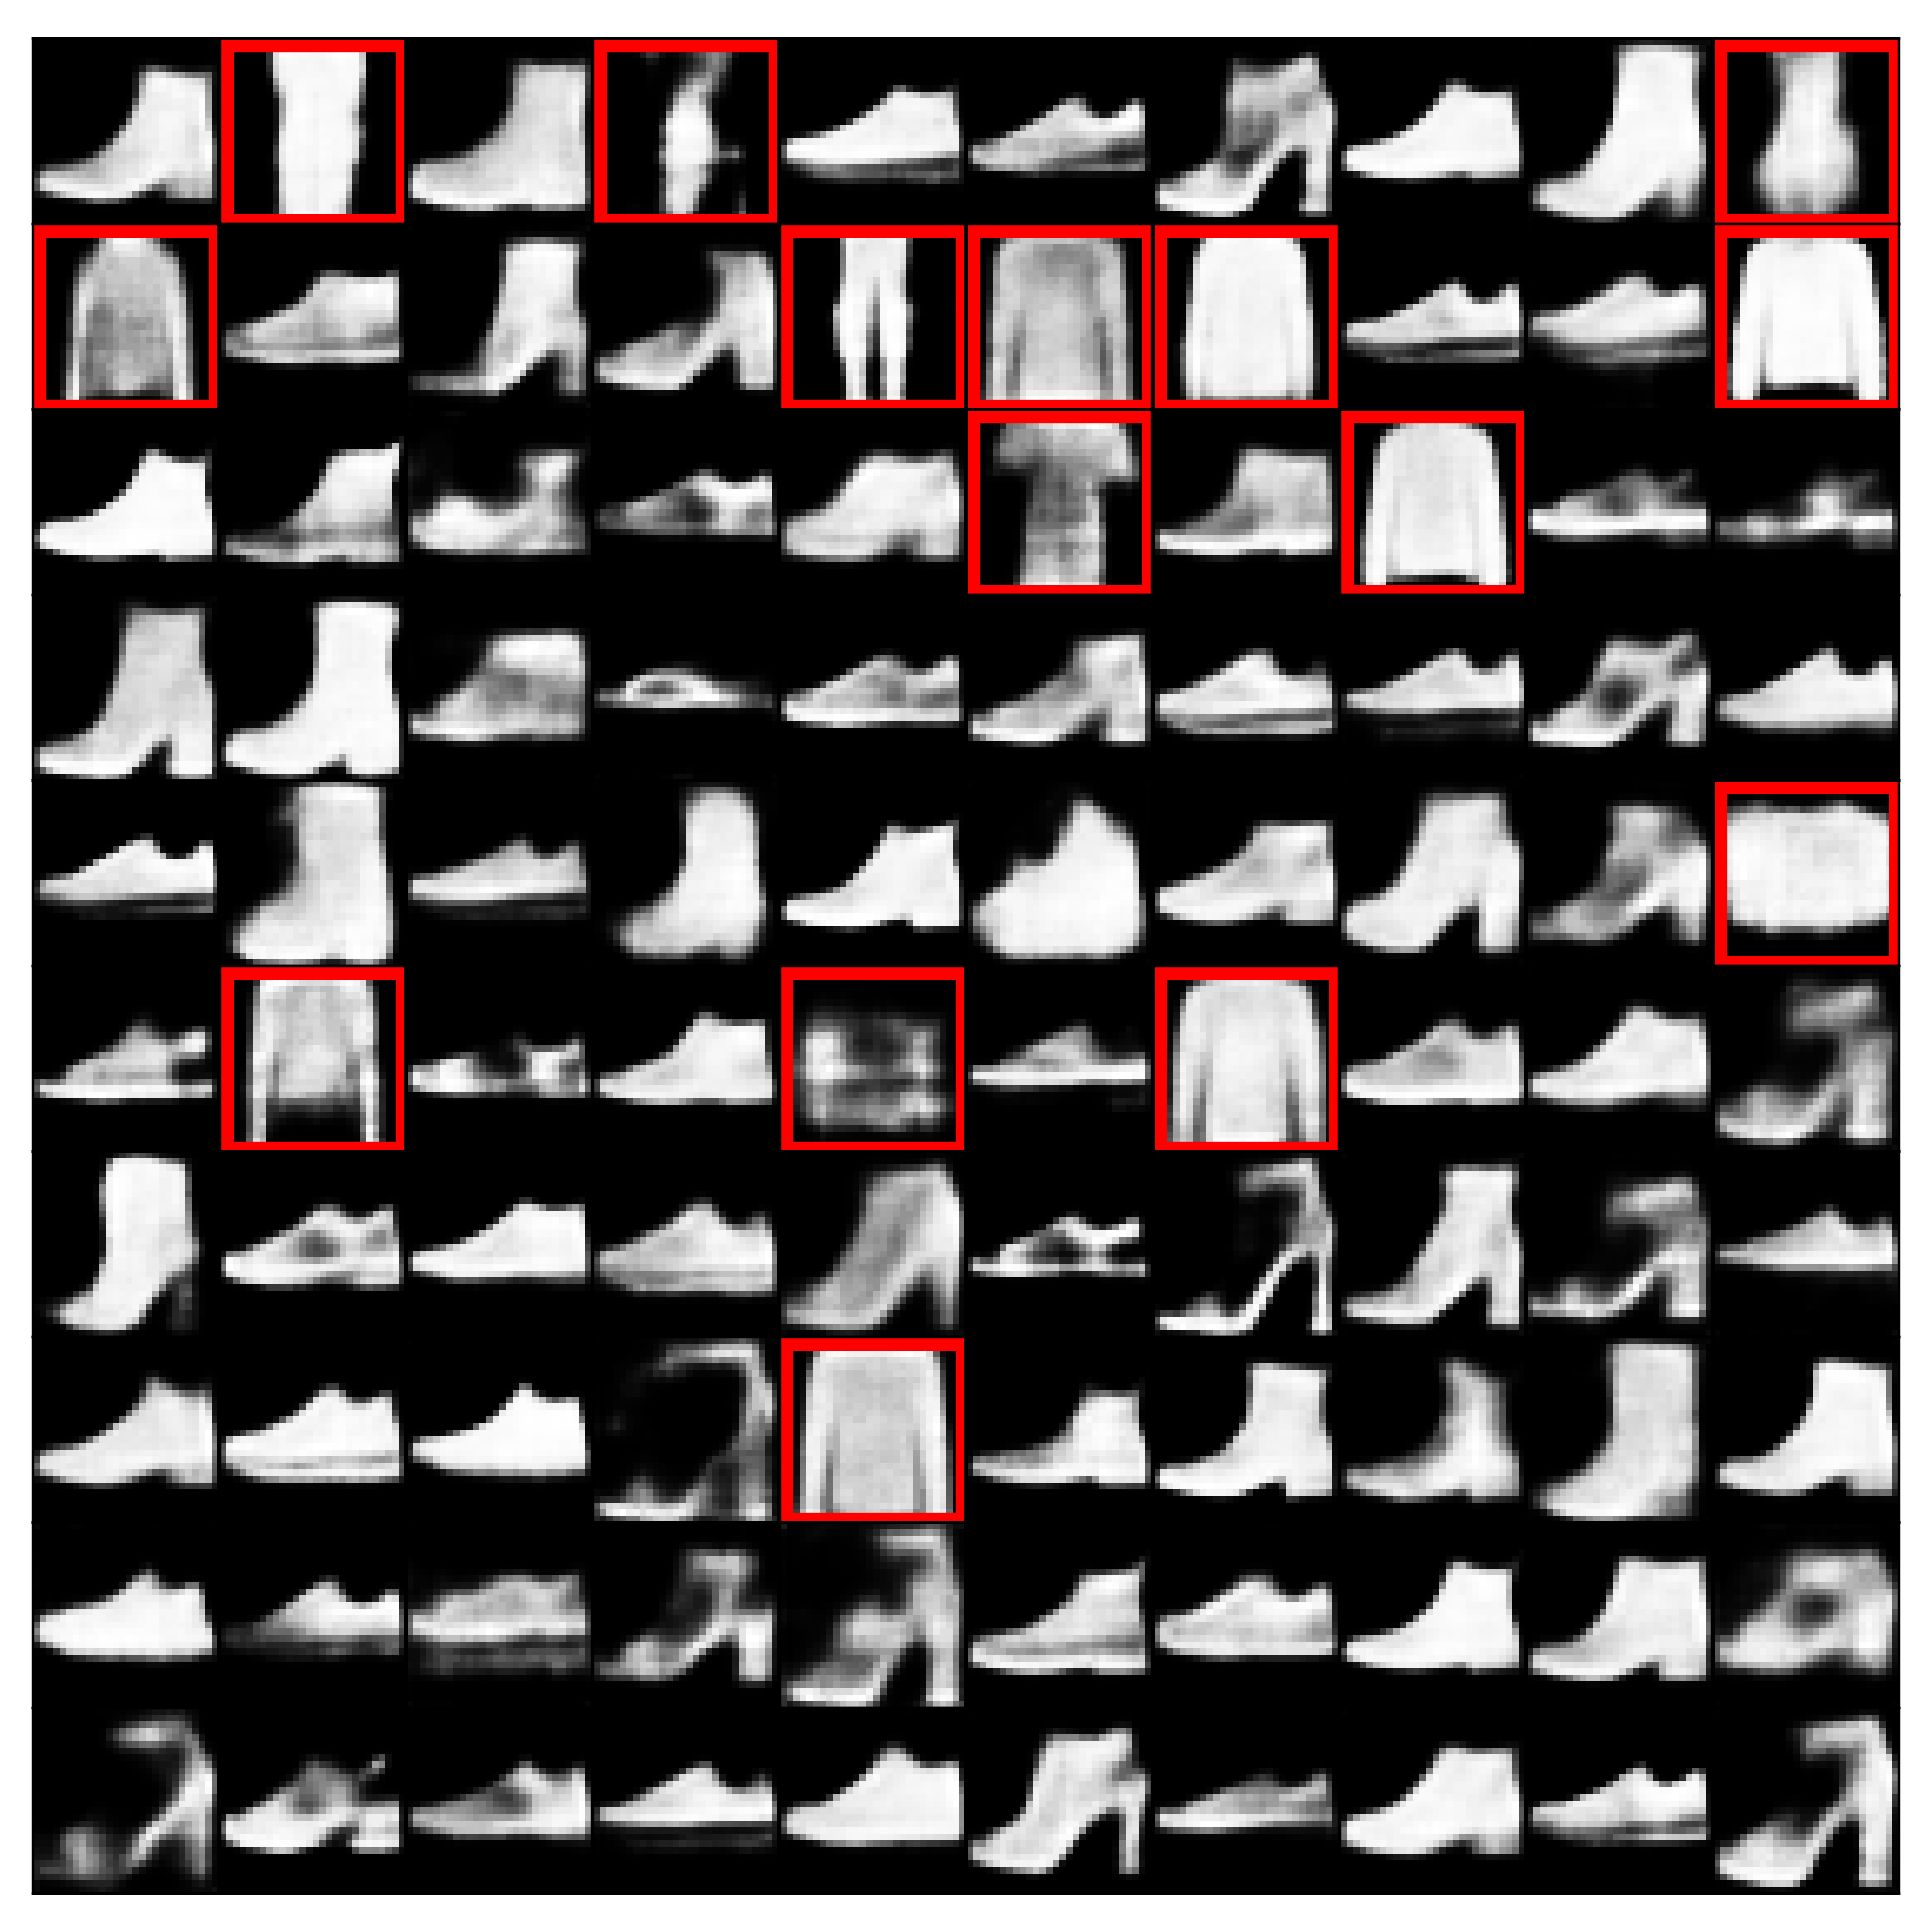
\includegraphics[width=0.8\textwidth]{Figures/Methods/FSM_random_generation.png}
%     \end{subfigure}
%     \hfill
%     \begin{subfigure}{0.45\textwidth}
%         \centering
%         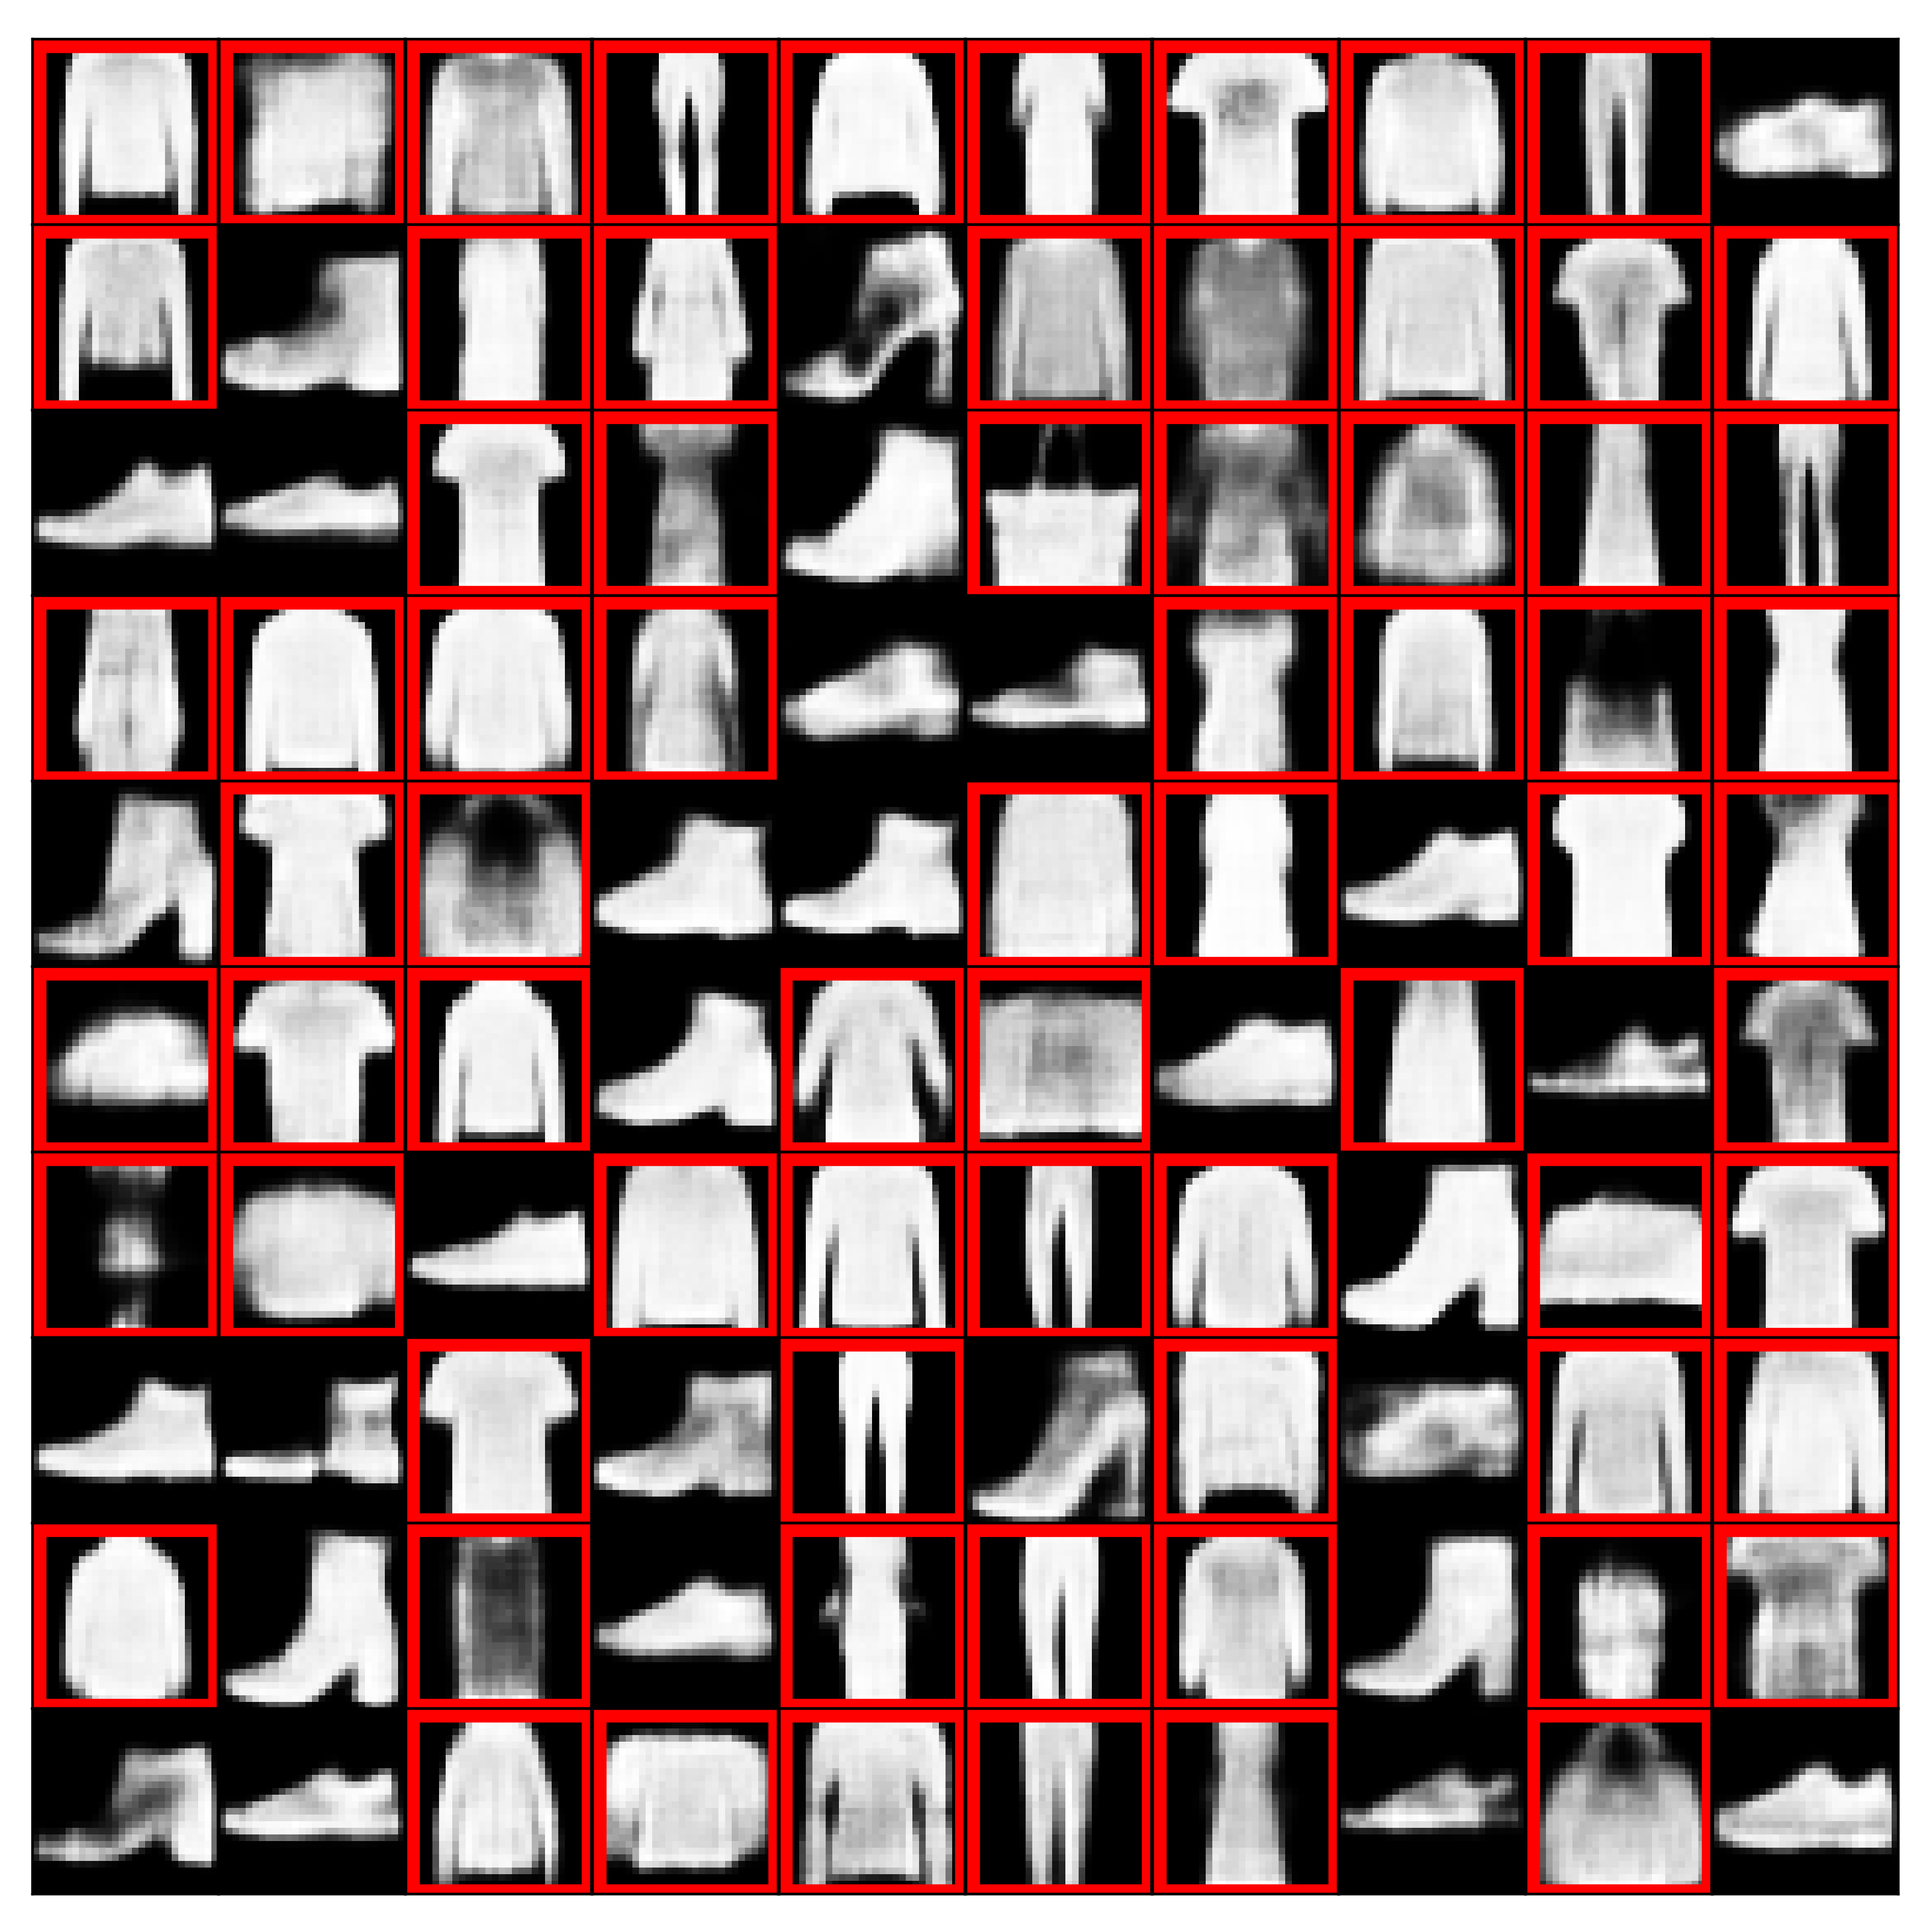
\includegraphics[width=0.8\textwidth]{Figures/Methods/FSM_invw_random_generation.png}
%     \end{subfigure}
%     \caption{Random generation of unbalanced FashionMNIST dataset: vanilla Gen-RKM (right) and Gen-RKM with inverse frequency sampling (left)}
%     \label{fig-ubfs}
% \end{figure}

\subsection{Effect of inverse frequency sampling on conditional generation in Gen-RKM}
We examine the effectiveness of conditional generation (described in Section \ref{subsec-methods-congen}) within the framework of Gen-RKM in this section. Conditional generations on unbalanced MNIST and unbalanced Fashion MNIST are visualized in Figure \ref{fig-IWS-congen}. Unsurprisingly, the generation quality could be worse if the generation is conditioned on a minority class, and it is likely to incorrectly generate images from other classes. For example, if one inspects the fifth column (generation conditioned on digit 4) in the MNIST case, the generation resembles digit 9 instead of digit 4. This issue is caused by the distorted latent space due to unbalanced data, latent representations of minority modes could be blurred or mixed with other majority modes, leading to failed conditional generation for underrepresented groups. This problem can now be resolved by adapting Gen-RKM with inverse frequency sampling. As shown in the right side of Figure \ref{fig-IWS-congen}, correct and clearer conditional generation can be obtained. By cleverly combining inverse frequency sampling with conditional generation, one can augment minority classes even from highly unbalanced training data.
\FloatBarrier
\begin{figure}[ht]
    \centering
    \begin{subfigure}{0.45\textwidth}
        \centering
        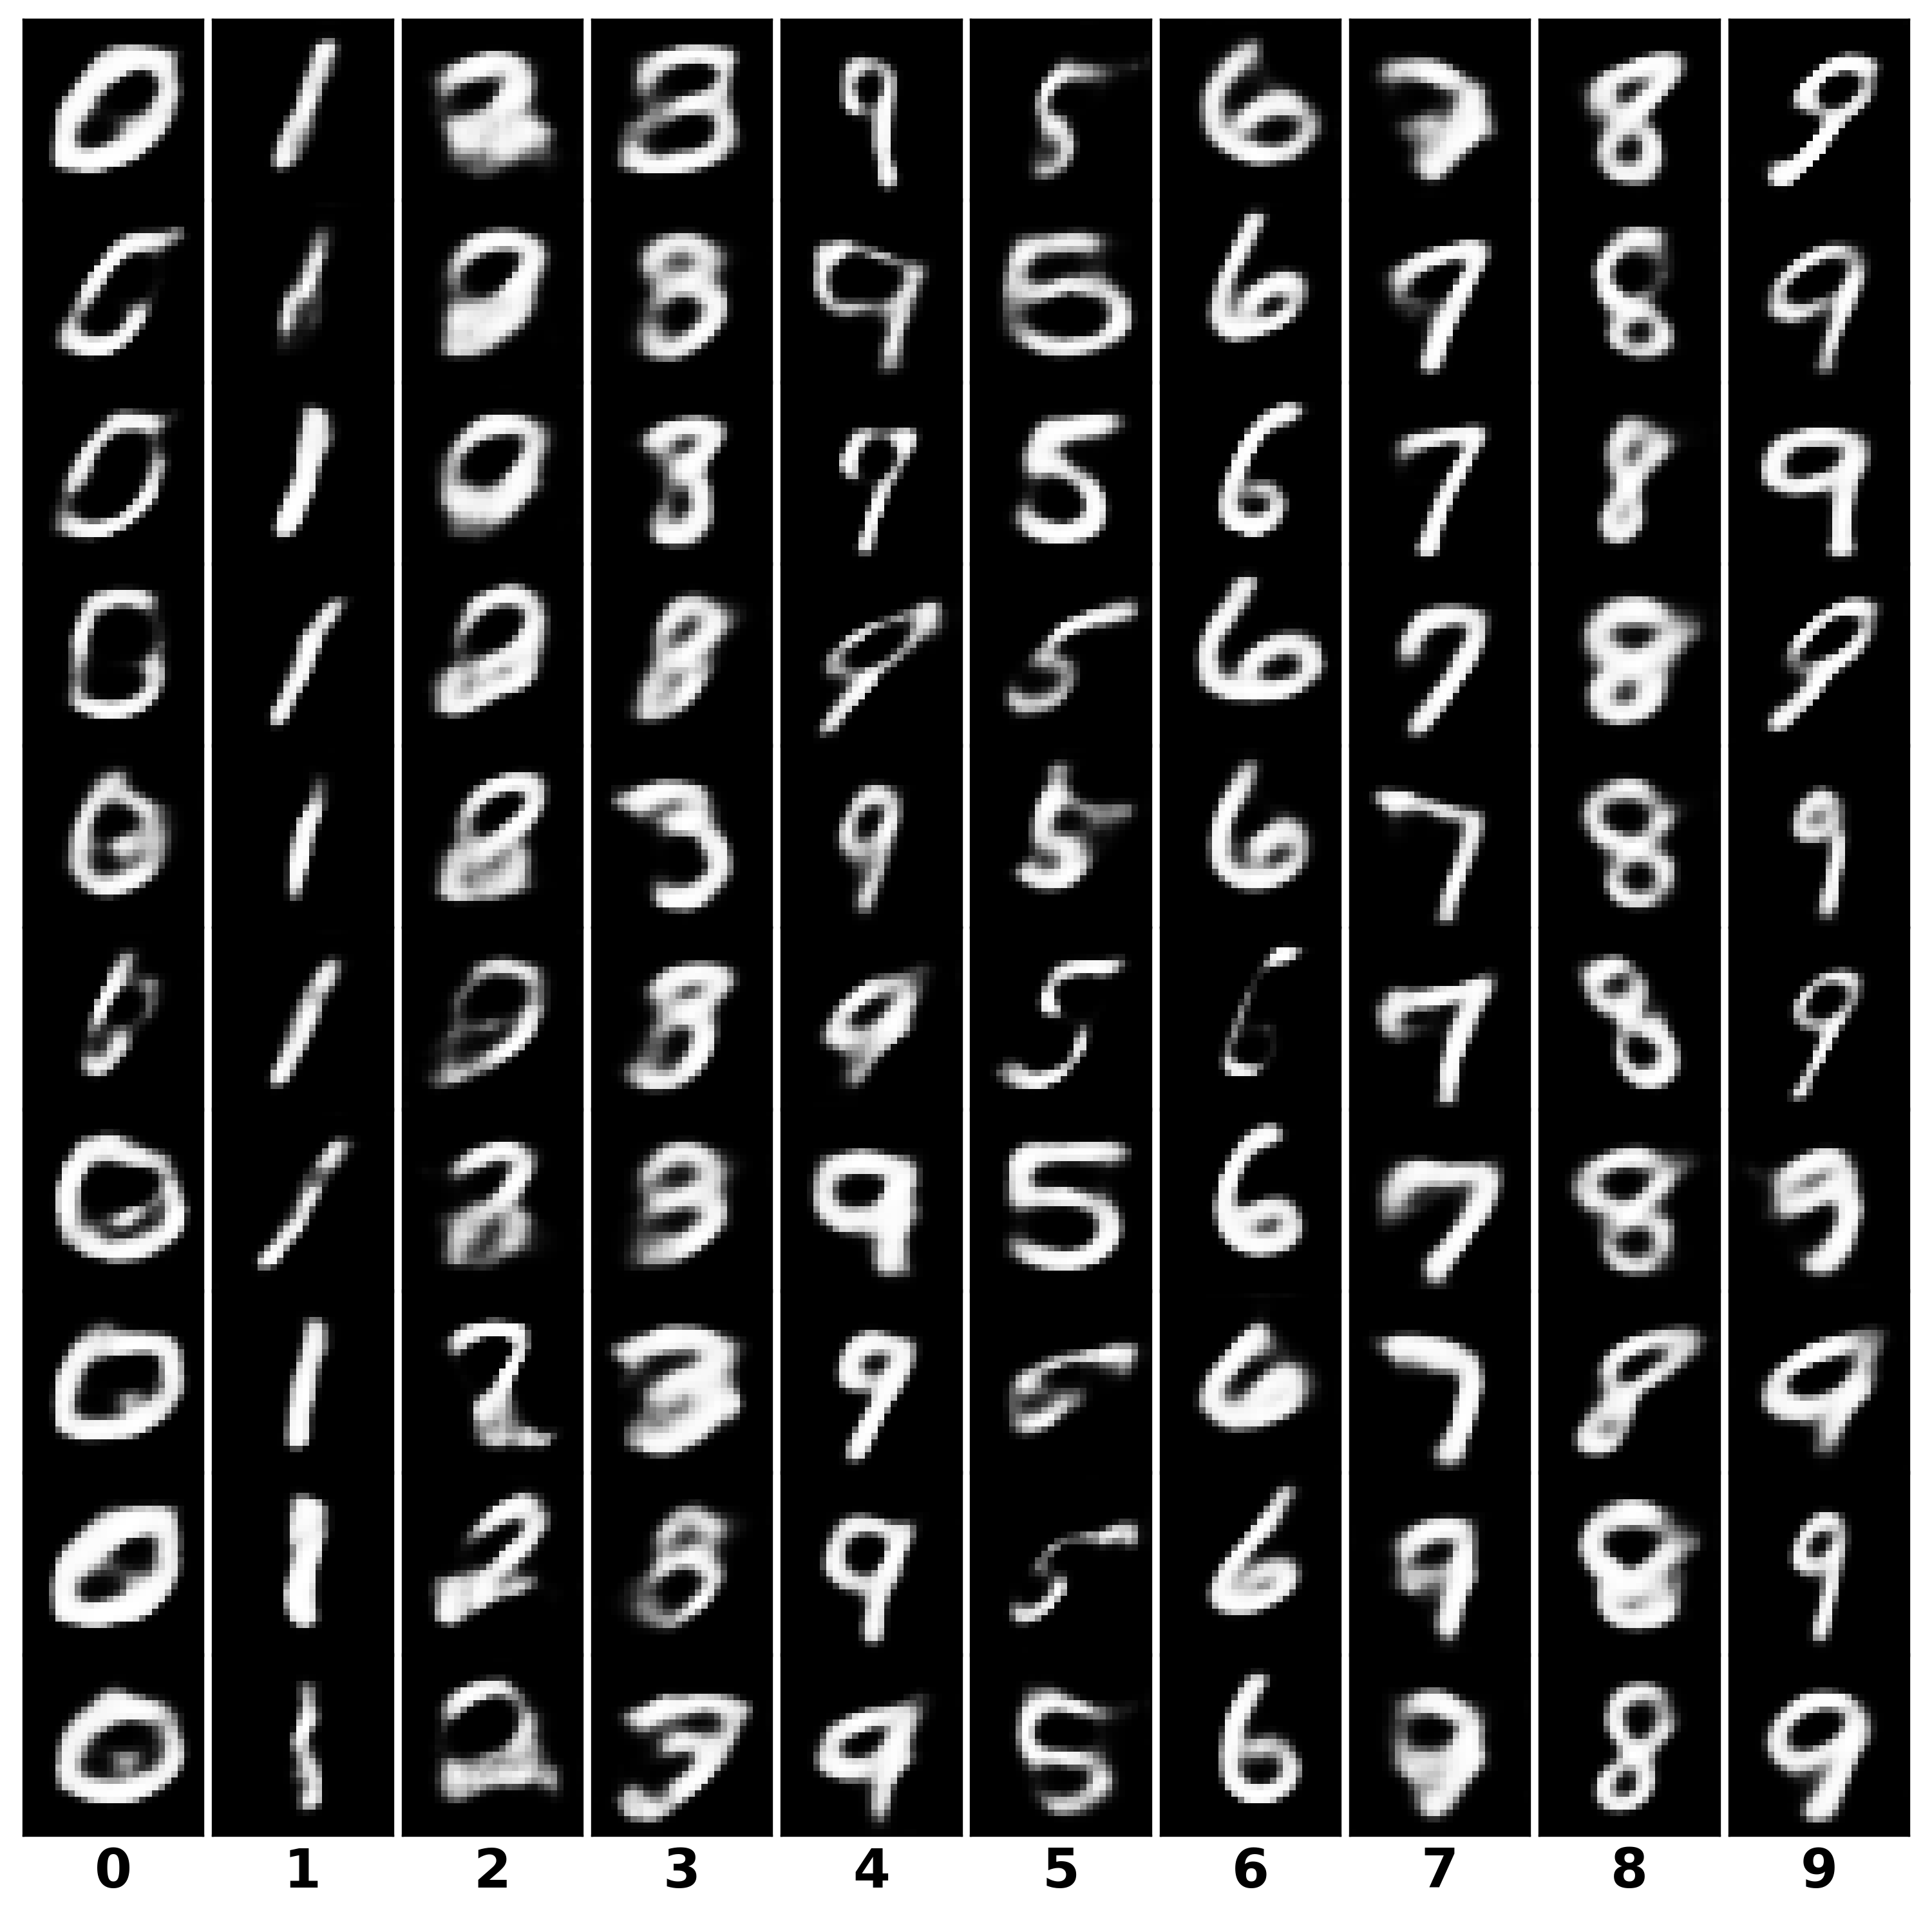
\includegraphics[width=0.7\textwidth]{Figures/Methods/RKM-congen-ubMNIST.png}
    \end{subfigure}
    \hfill
    \begin{subfigure}{0.45\textwidth}
        \centering
        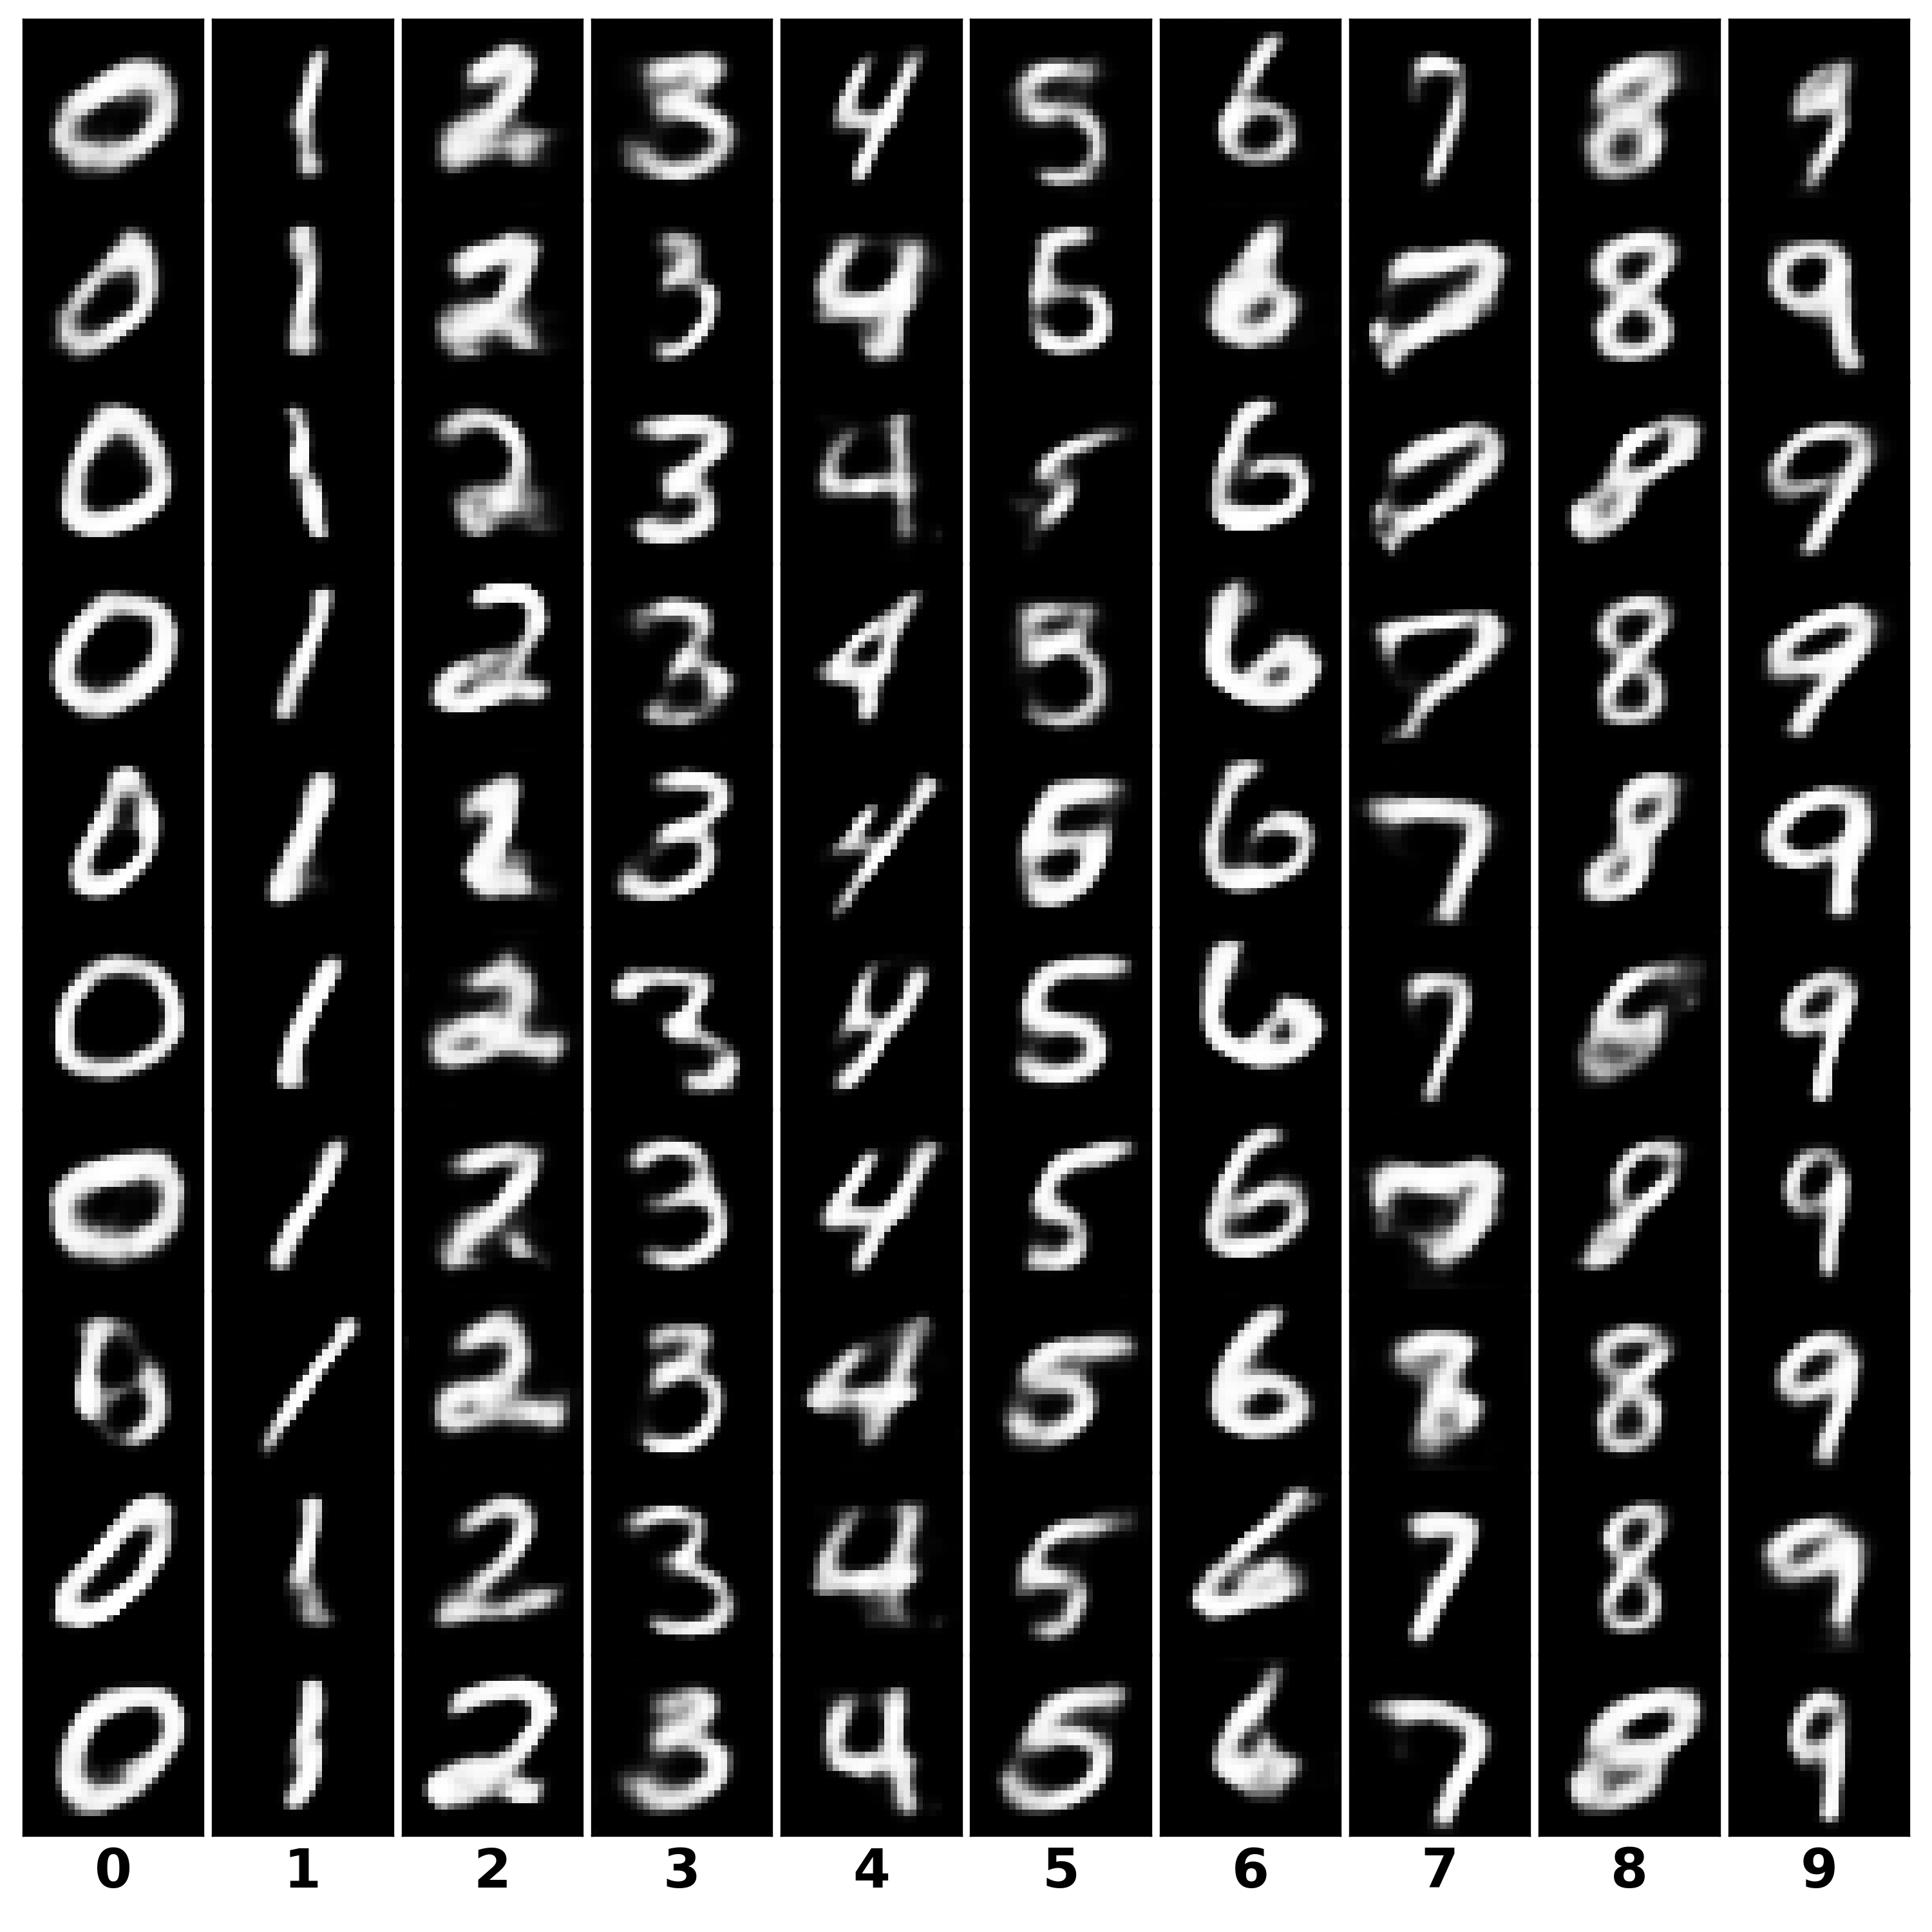
\includegraphics[width=0.7\textwidth]{Figures/Methods/IWRKM-congen-ubMNIST.png}
    \end{subfigure}
    \hfill
    \begin{subfigure}{0.45\textwidth}
        \centering
        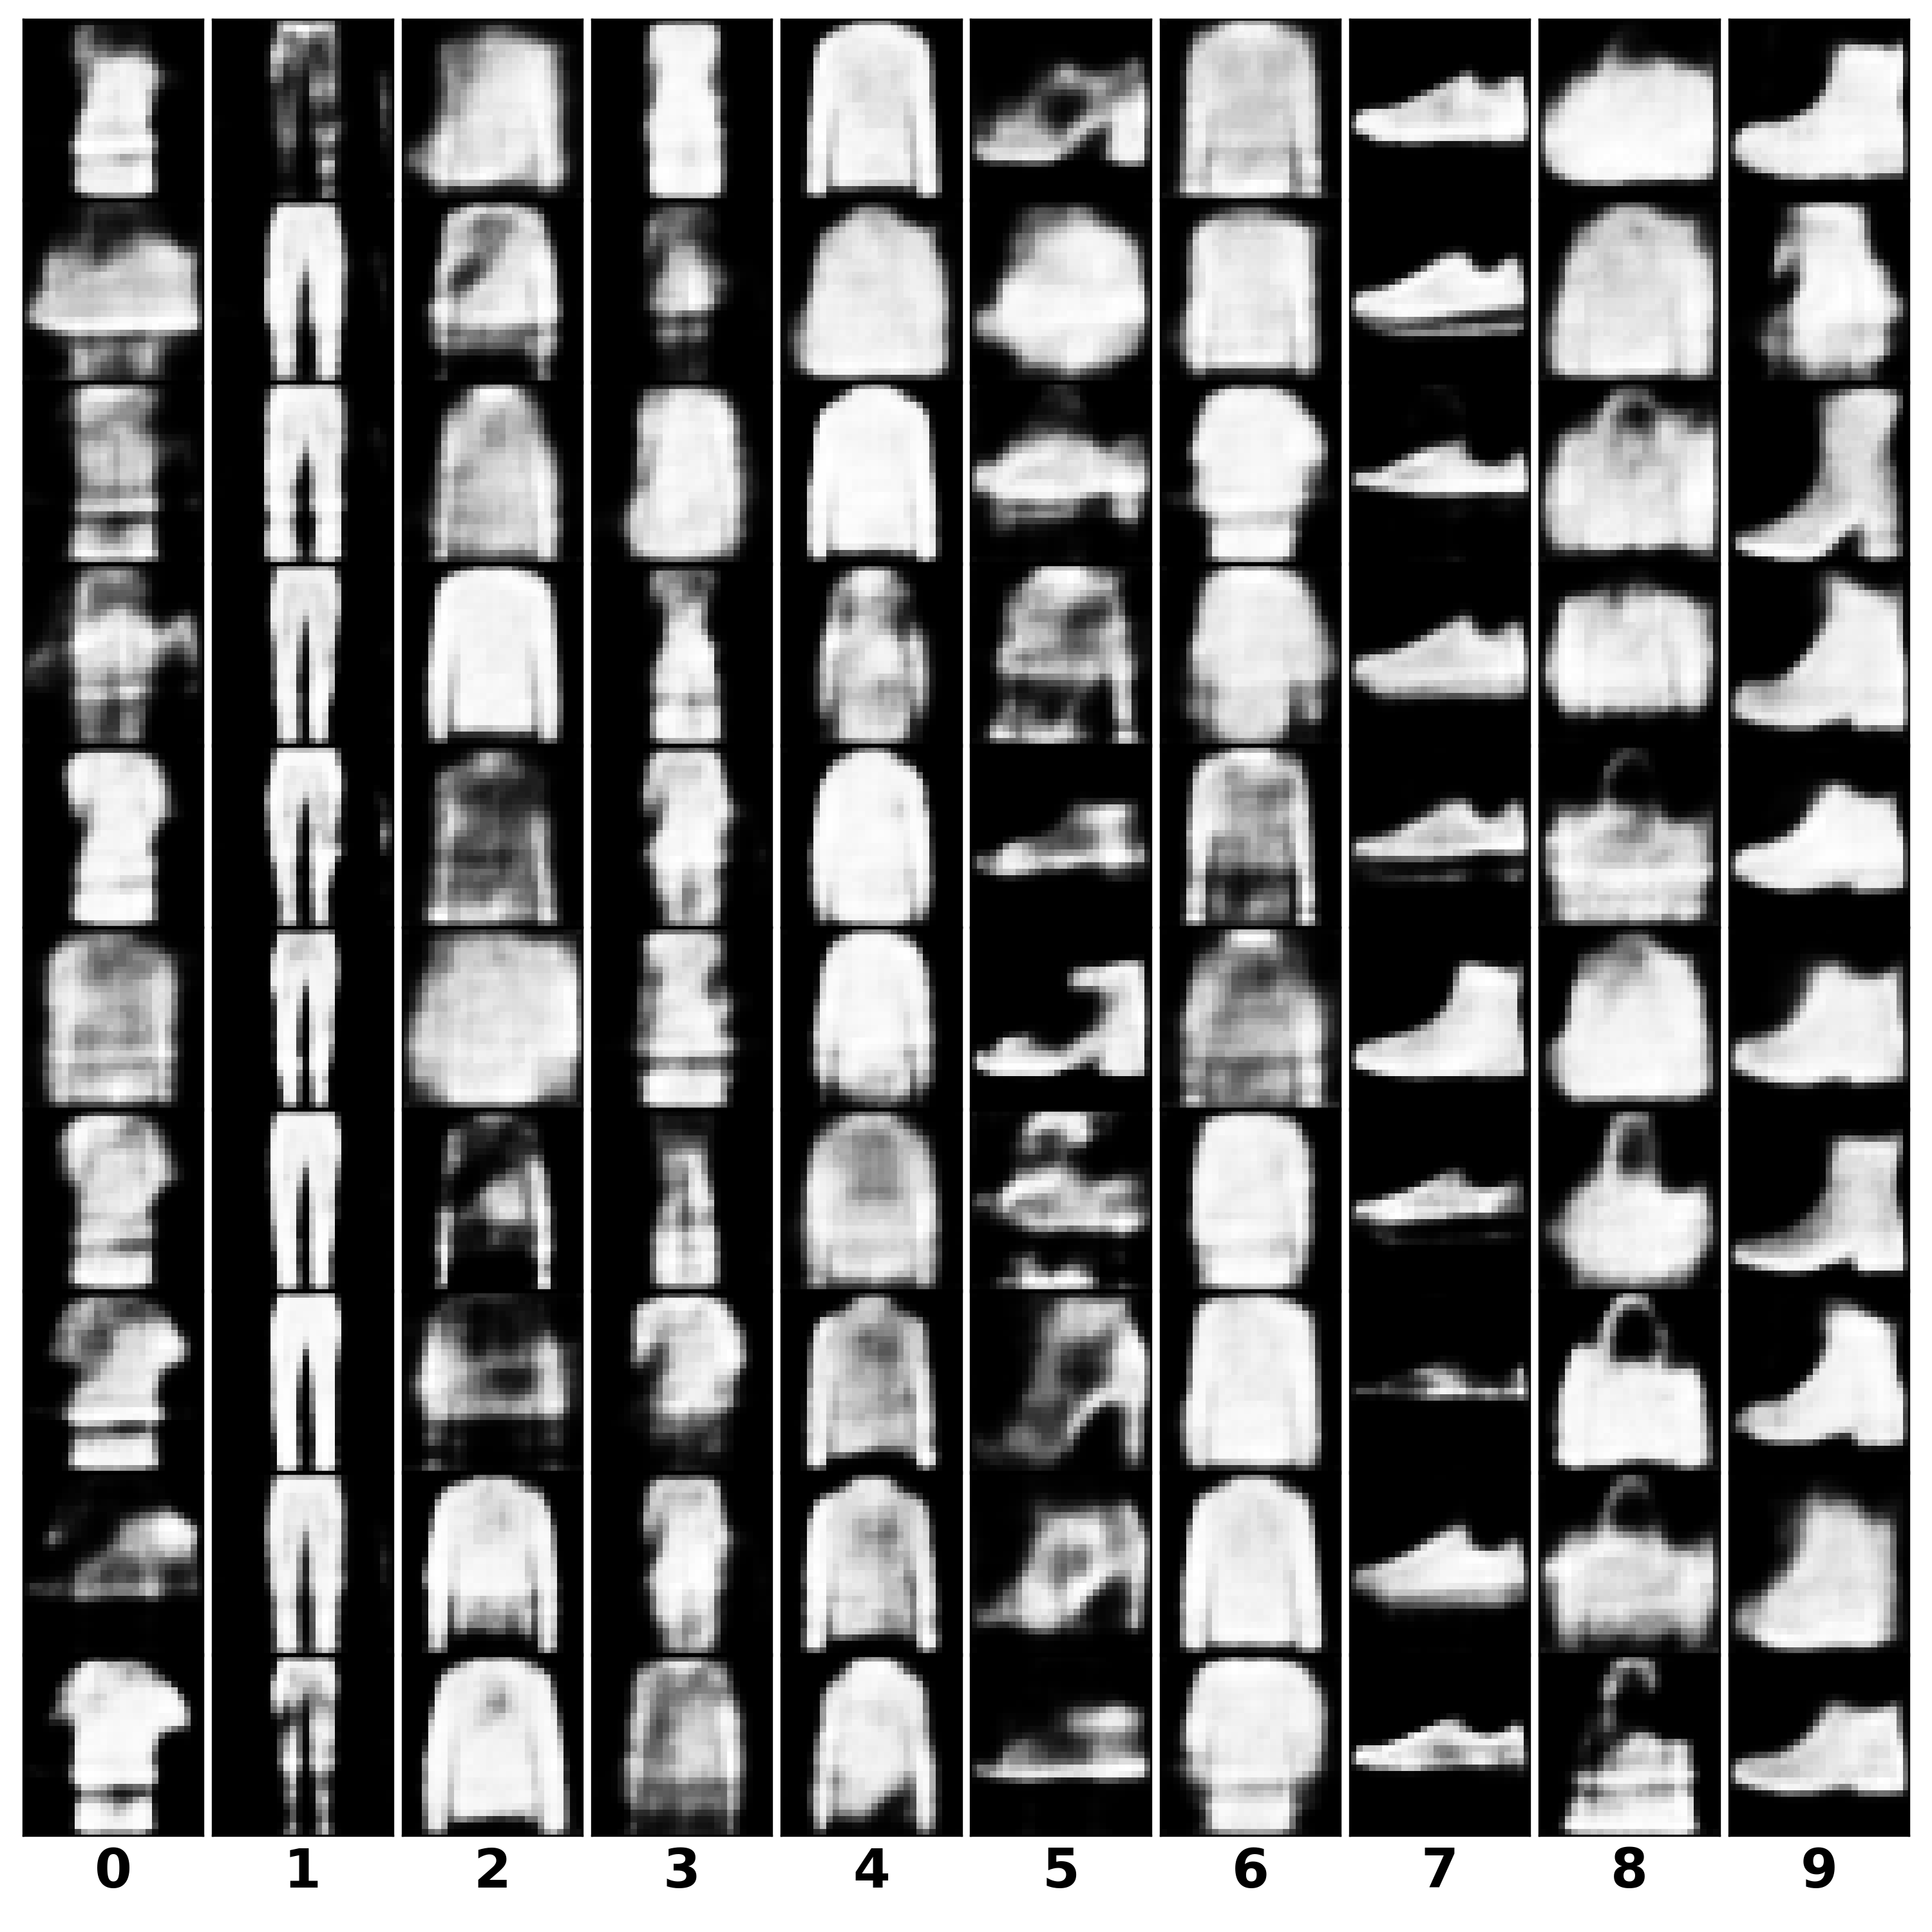
\includegraphics[width=0.7\textwidth]{Figures/Methods/RKM-congen-ubFashion.png}
    \end{subfigure}
    \hfill
    \begin{subfigure}{0.45\textwidth}
        \centering
        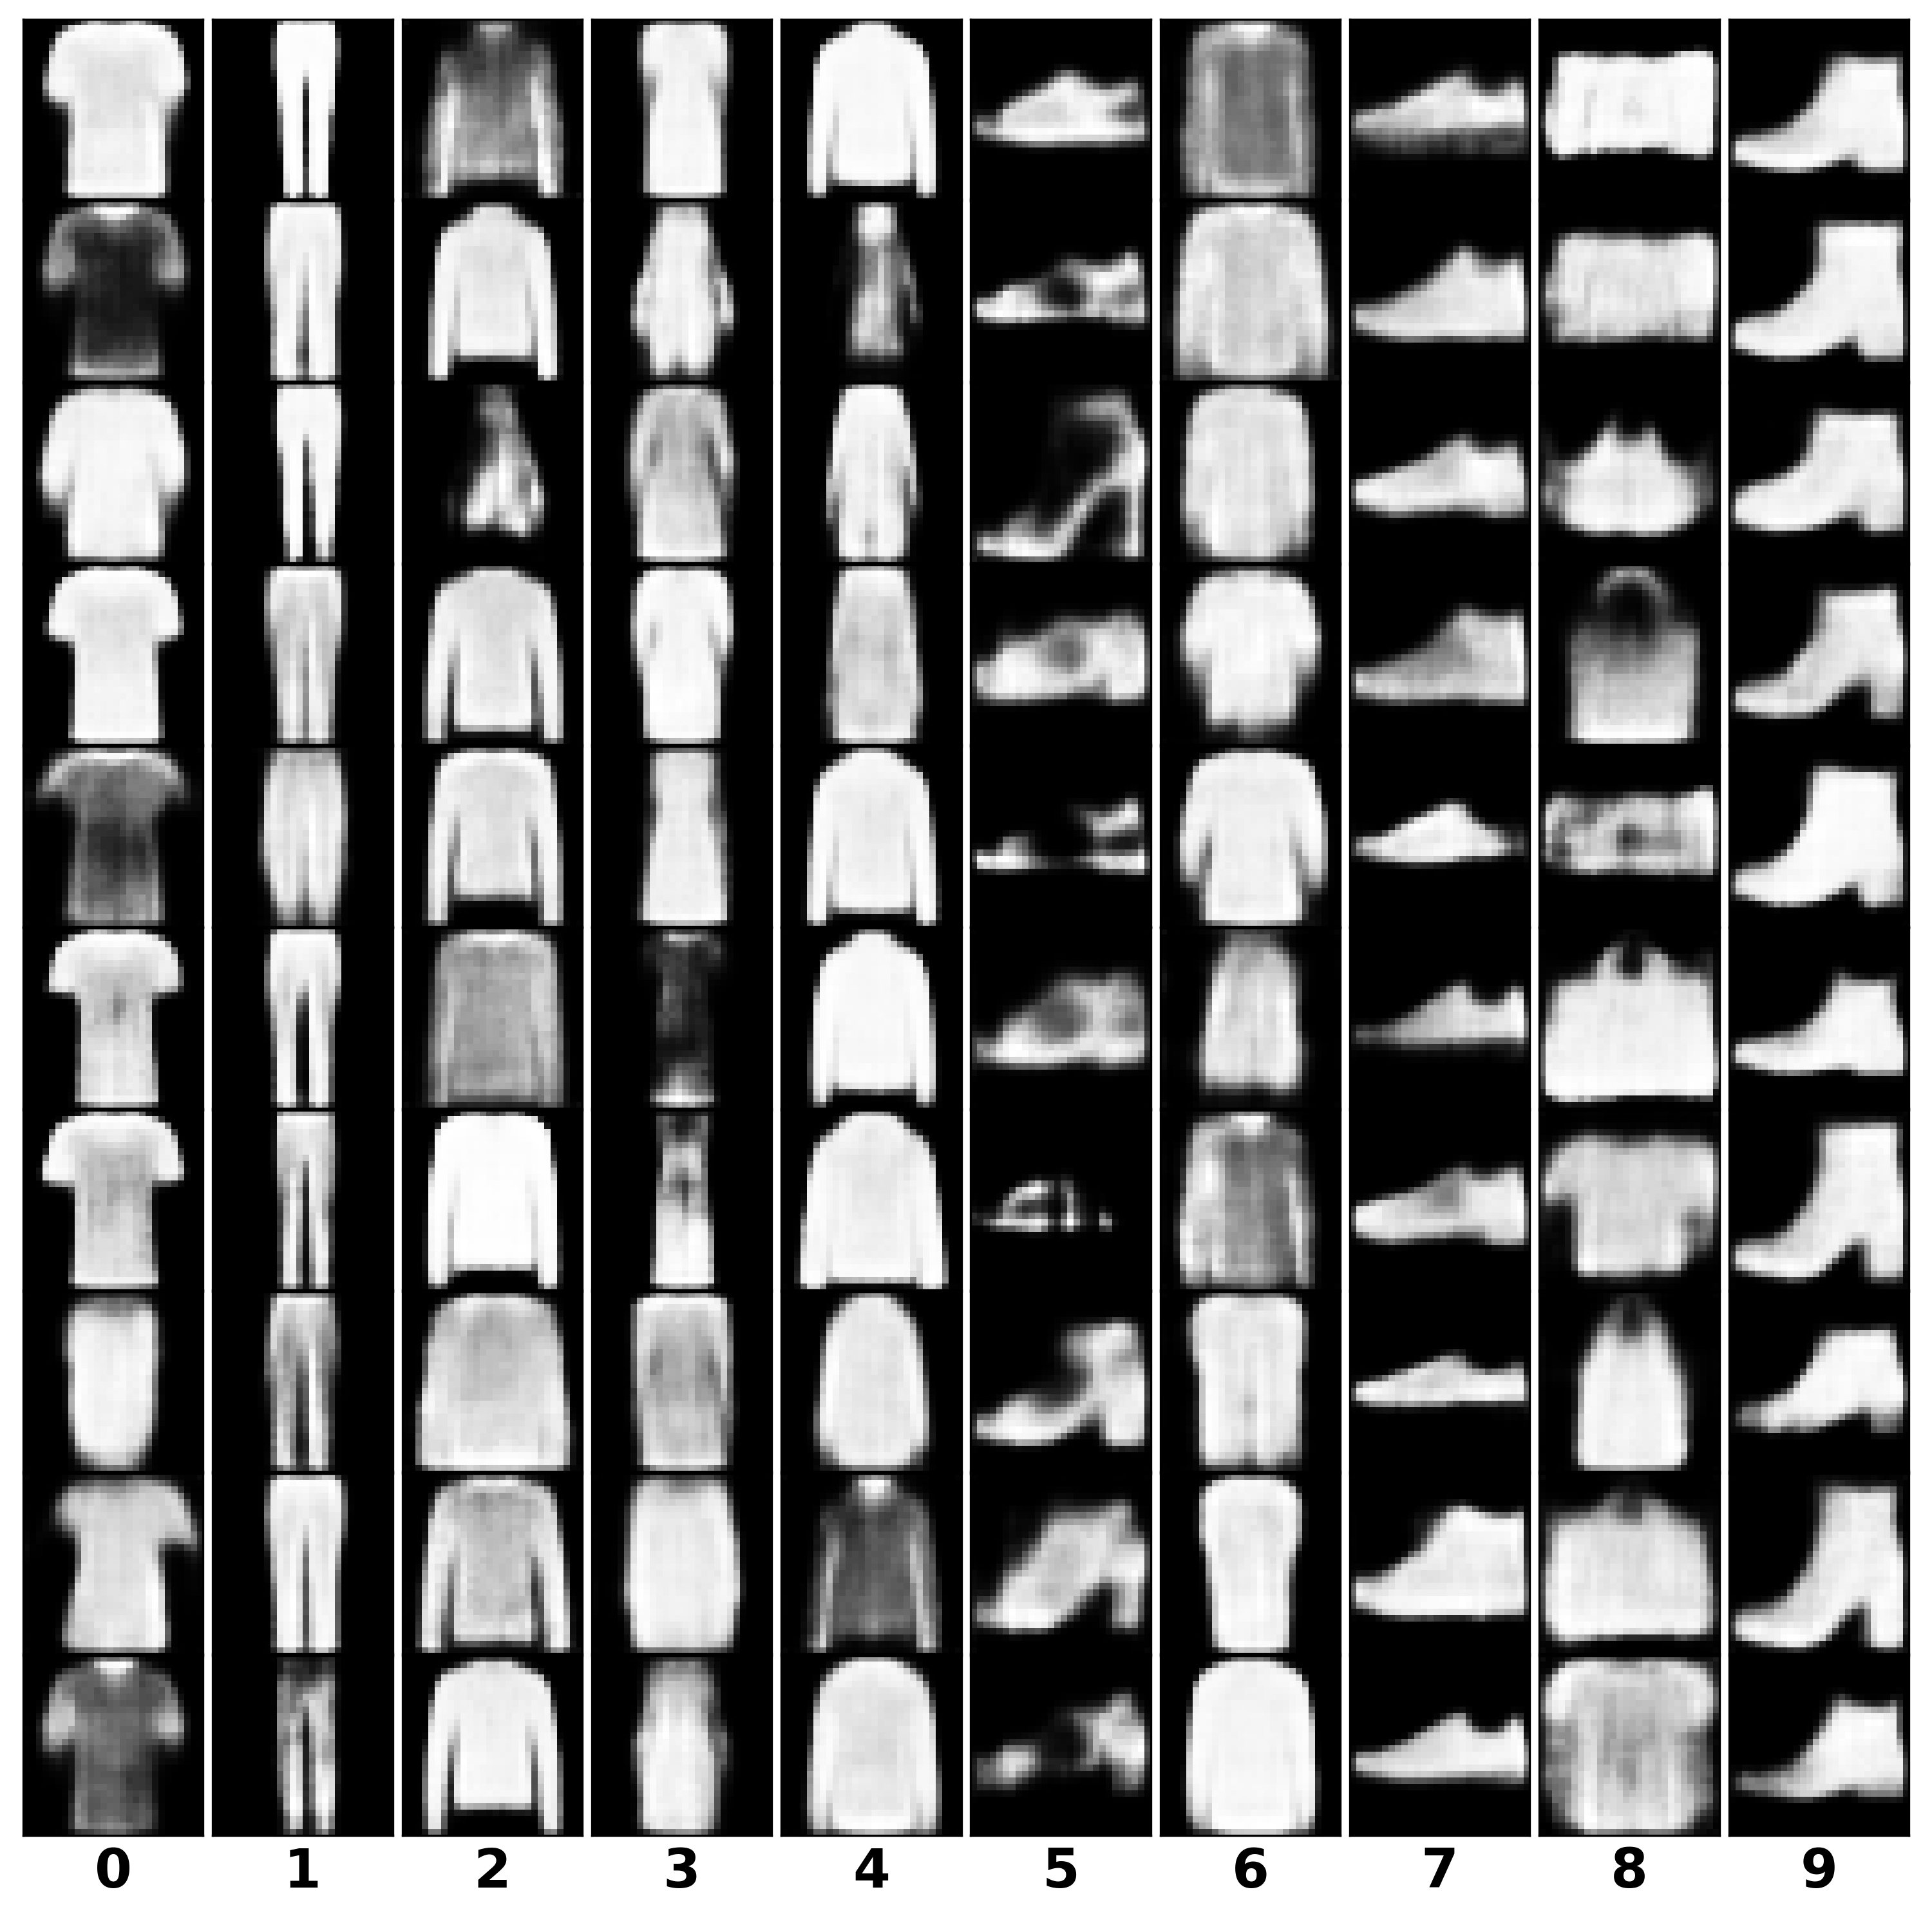
\includegraphics[width=0.7\textwidth]{Figures/Methods/IWRKM-congen-ubFashion.png}
    \end{subfigure}
    \caption{Conditional generations produced by multi-view Gen-RKM on the unbalanced MNIST dataset (top row) and the unbalanced Fashion MNIST dataset (bottom row). Figures in left column is generated by vanilla Gen-RKM, and figures in the right column are generated by Gen-RKM adapted with inverse frequency sampling. Images in each column of each figure are generated conditionally on a particular label. Imbalance ratios for both datasets are set to 0.1.}
    \label{fig-IWS-congen}
\end{figure}
\FloatBarrier

\section{Experiments on weighted sampling schemes under unsupervised setting}
\label{sec-expr-unsupervised}
In this section, we investigate the effectiveness of different diversity sampling schemes under unsupervised settings where no label information is provided during the training phase. Notice that label information is still required only for the purpose of evaluation. We start by evaluating RLS sampling in Gen-RKM on a toy 2D dataset in Section \ref{subsec-ringgrid}. Next, Section \ref{subsec-expr-ubMNIST012} and \ref{subsec-expr-ubMNIST} describe the results of experiments on MNIST-related datasets. In addition, results on Fashion MNIST under a similar setting are presented in Section \ref{subsec-expr-Fashion}. Lastly, some additional studies are conducted in \ref{subsec-additional-studies}.

\subsection{Synthetic ring/grid dataset}
\label{subsec-ringgrid}
The generated samples from models trained both with and without RLS sampling (using a shared feature map) are presented in Figure \ref{2d-rkm-vis}. It is evident from the visualization that the RKM, when trained using uniform sampling, fails to generate a sufficient number of points for the first four minority modes in the Ring and the first ten minority modes in the Grid. This problem is effectively solved by employing RLS sampling. The improved sampling effectiveness is demonstrated through the comparison of the two generation distributions for the Ring dataset, as shown in Figure \ref{fig-ring-rkm}. Meanwhile, Table \ref{tab-2d} presents the results of the two variants of RLS sampling, the primal form (shared feature map) and the dual form (RBF kernel with $\sigma=0.15$), on 2D synthetic datasets. Here, “minority mean” refers to the average number of points generated in each minority mode, while “number modes” indicates how many modes have generated more than 50 points. Both the primal and dual forms of RLS sampling enhance mode coverage and substantially increase the generation count in the minority modes.

\begin{figure}[ht]
    \centering
    \begin{subfigure}{0.32\textwidth}
        \centering
        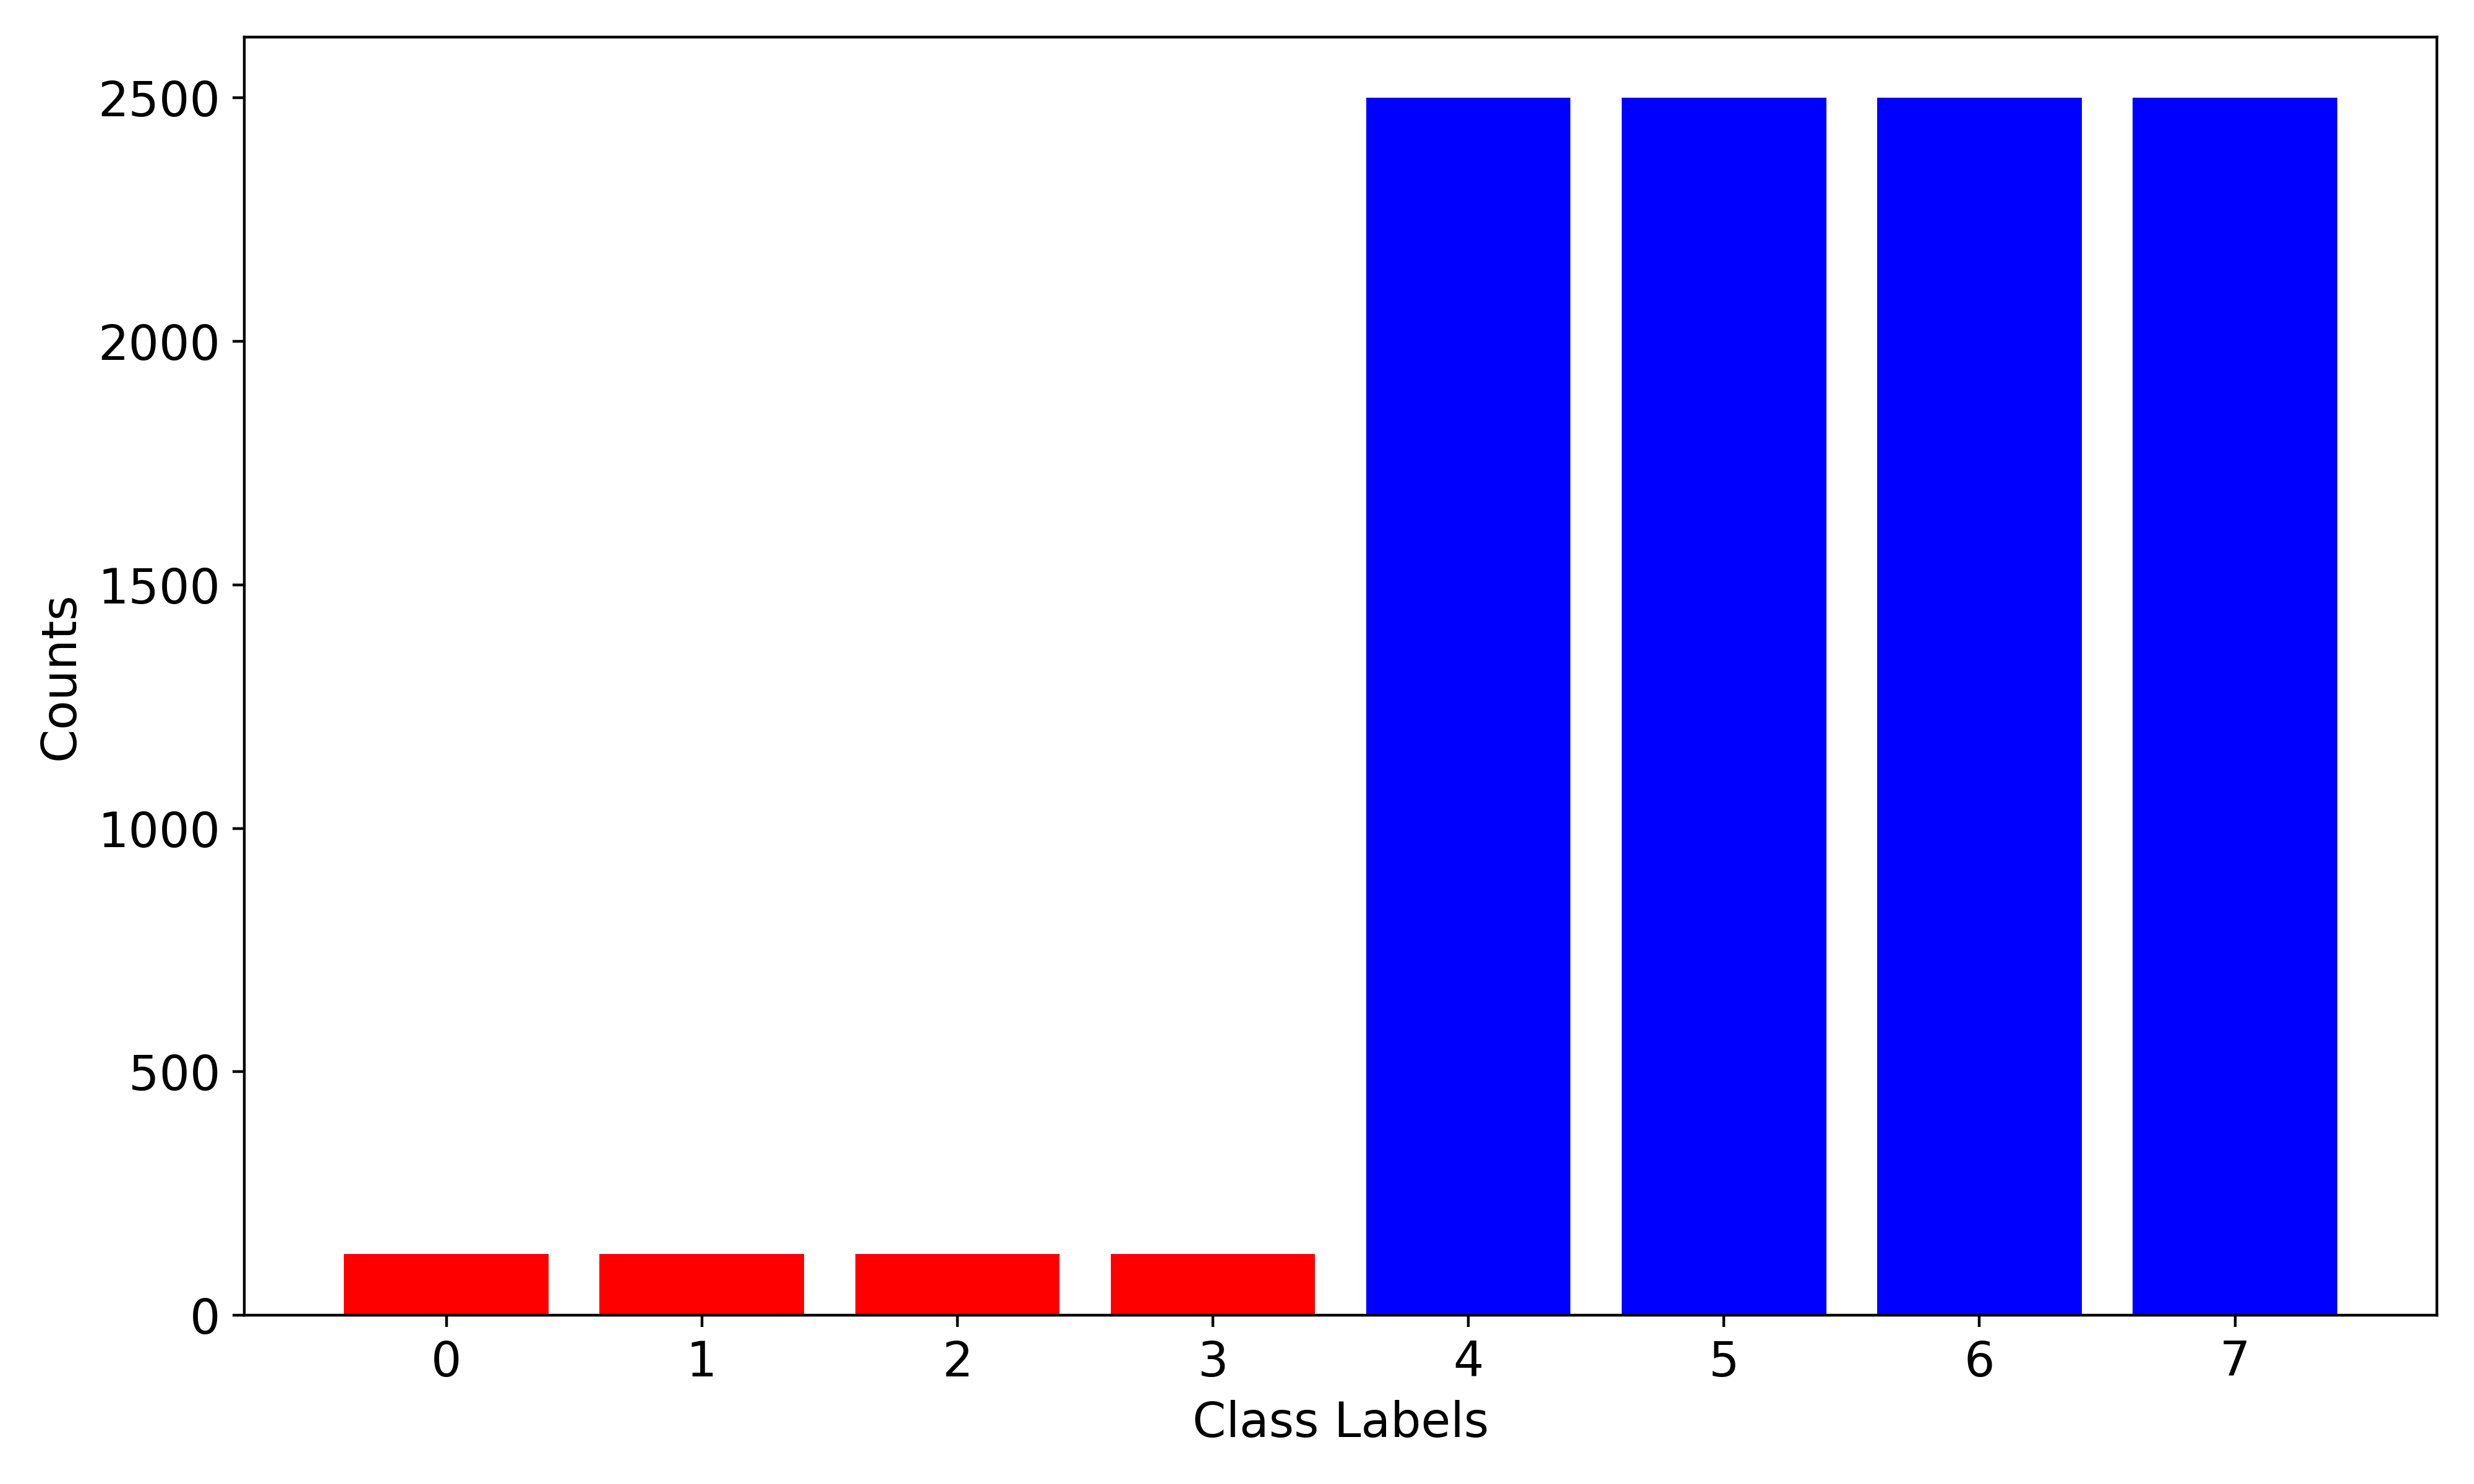
\includegraphics[width=0.9\textwidth]{Figures/Methods/ring_dis.png}
    \end{subfigure}
    %\hfill
    \begin{subfigure}{0.32\textwidth}
        \centering
        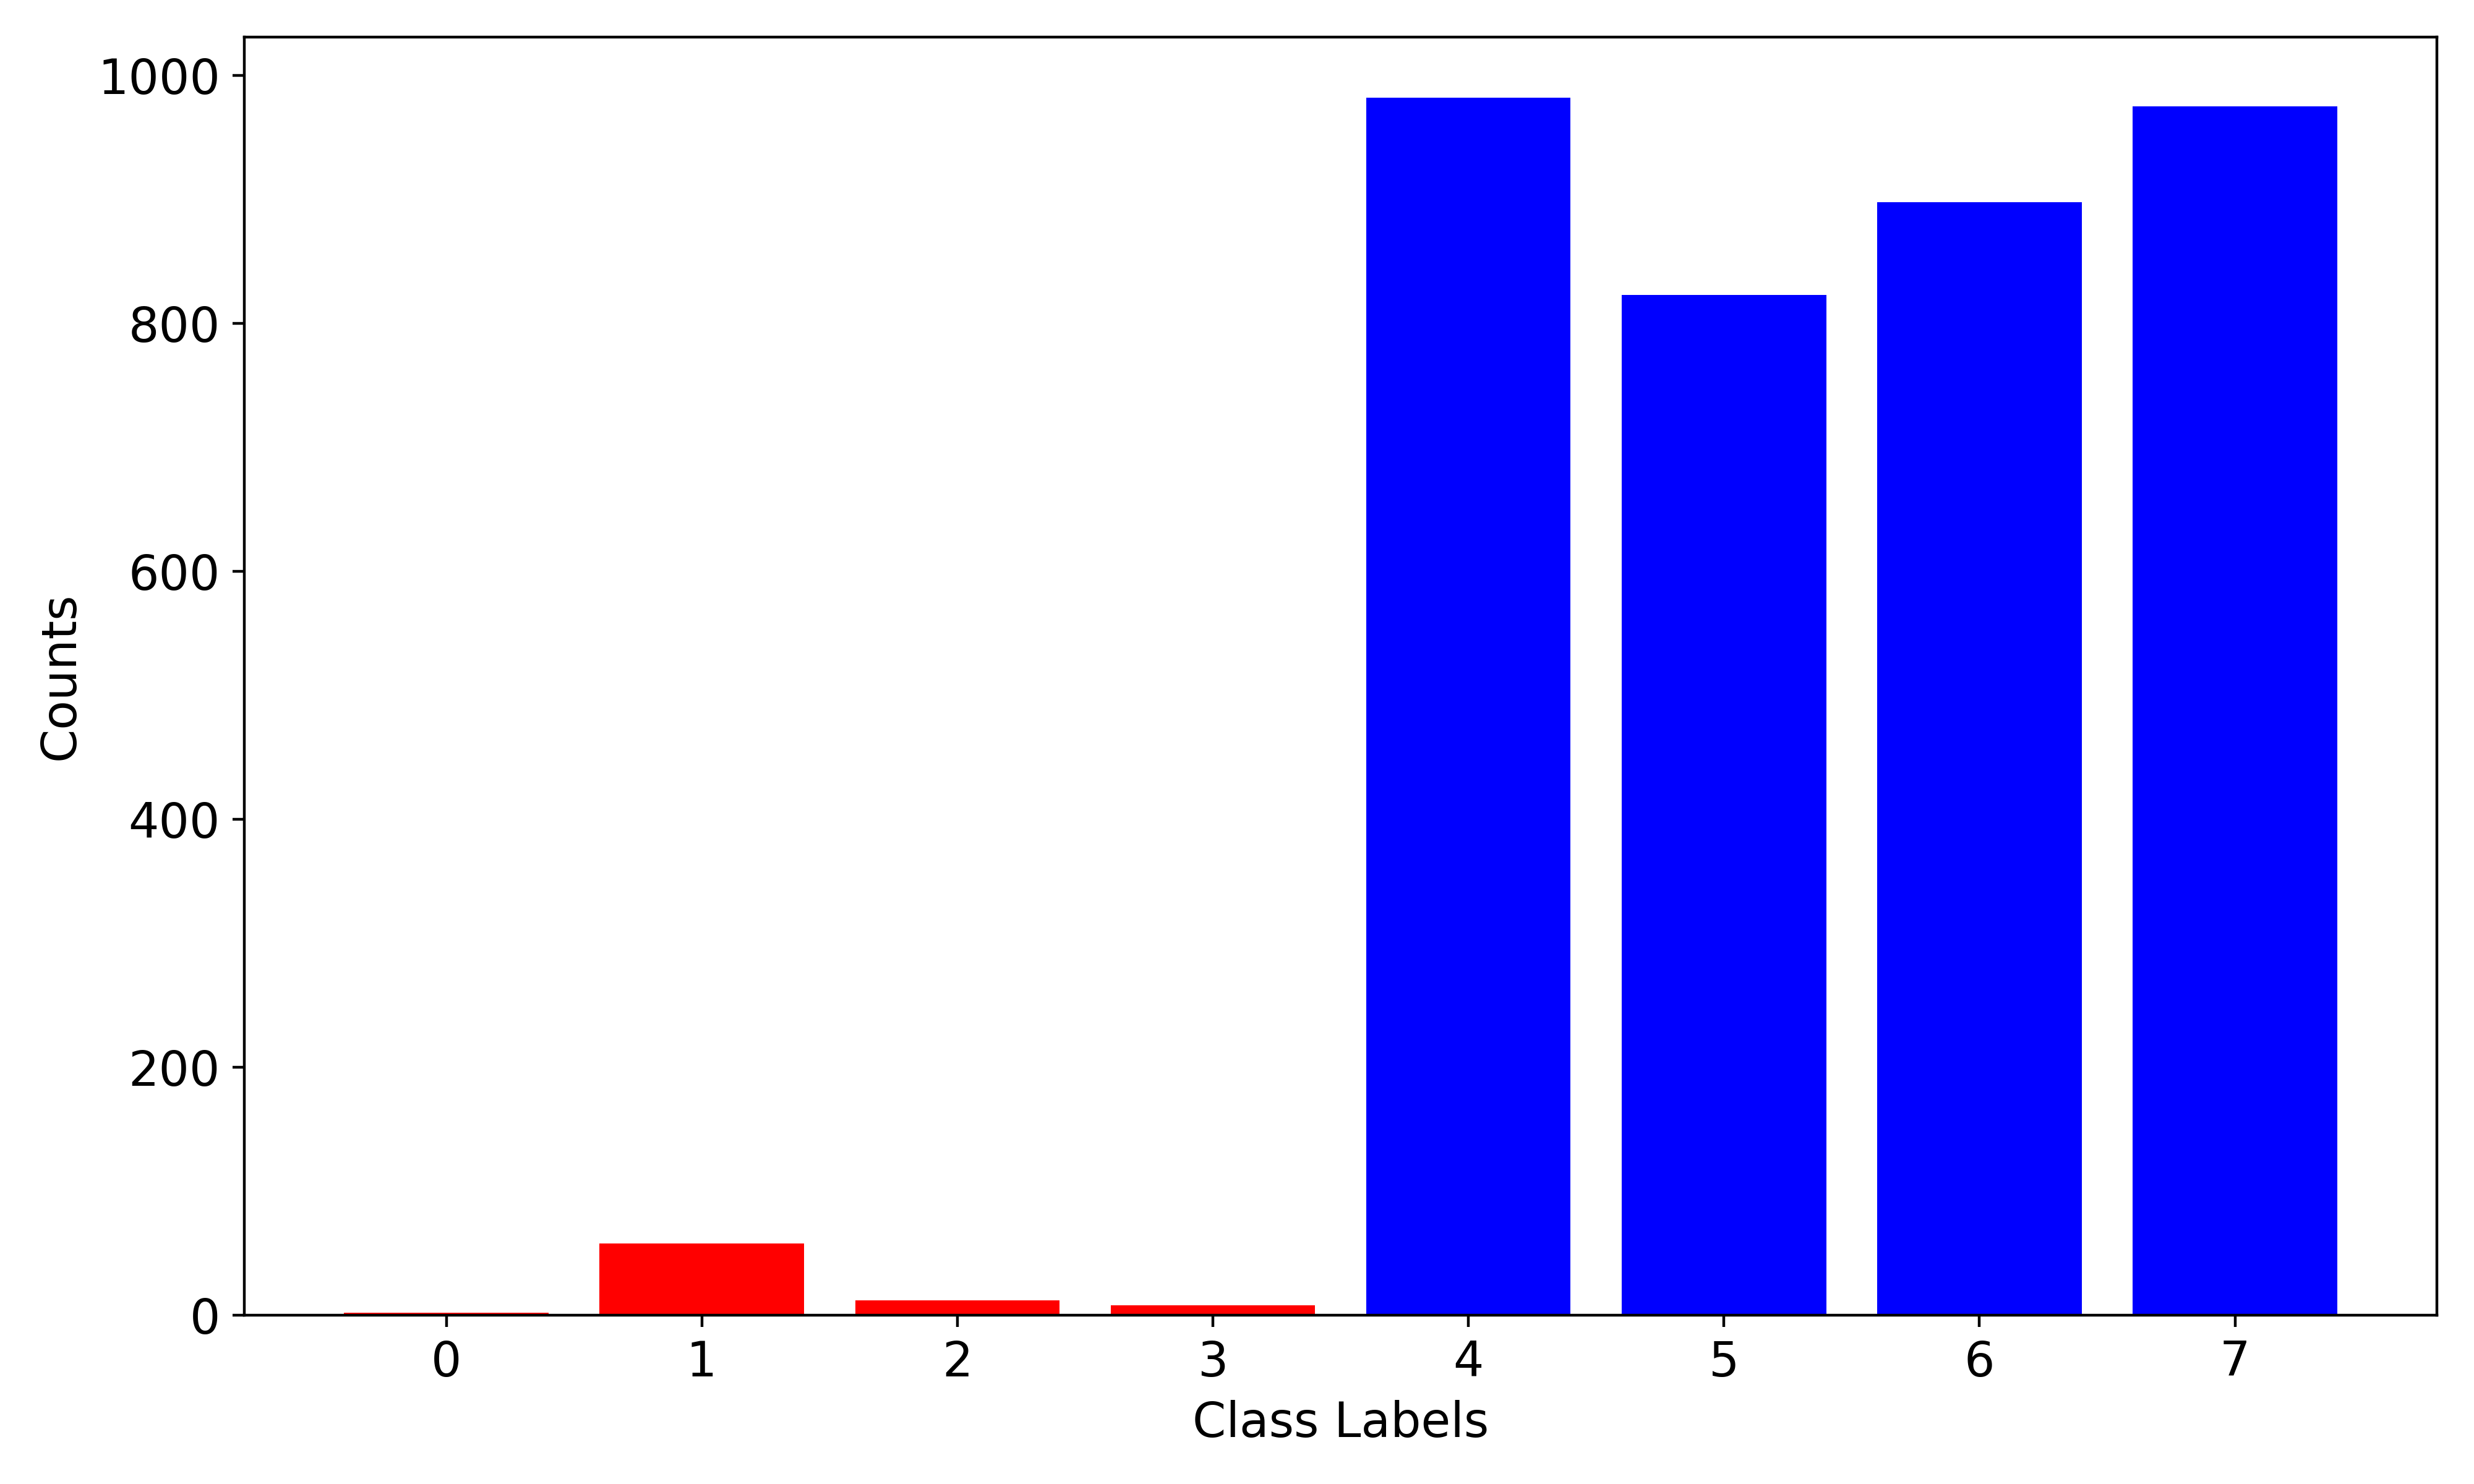
\includegraphics[width=0.9\textwidth]{Figures/Methods/ring_rkm.png}
    \end{subfigure}
    %\hfill
    \begin{subfigure}{0.32\textwidth}
        \centering
        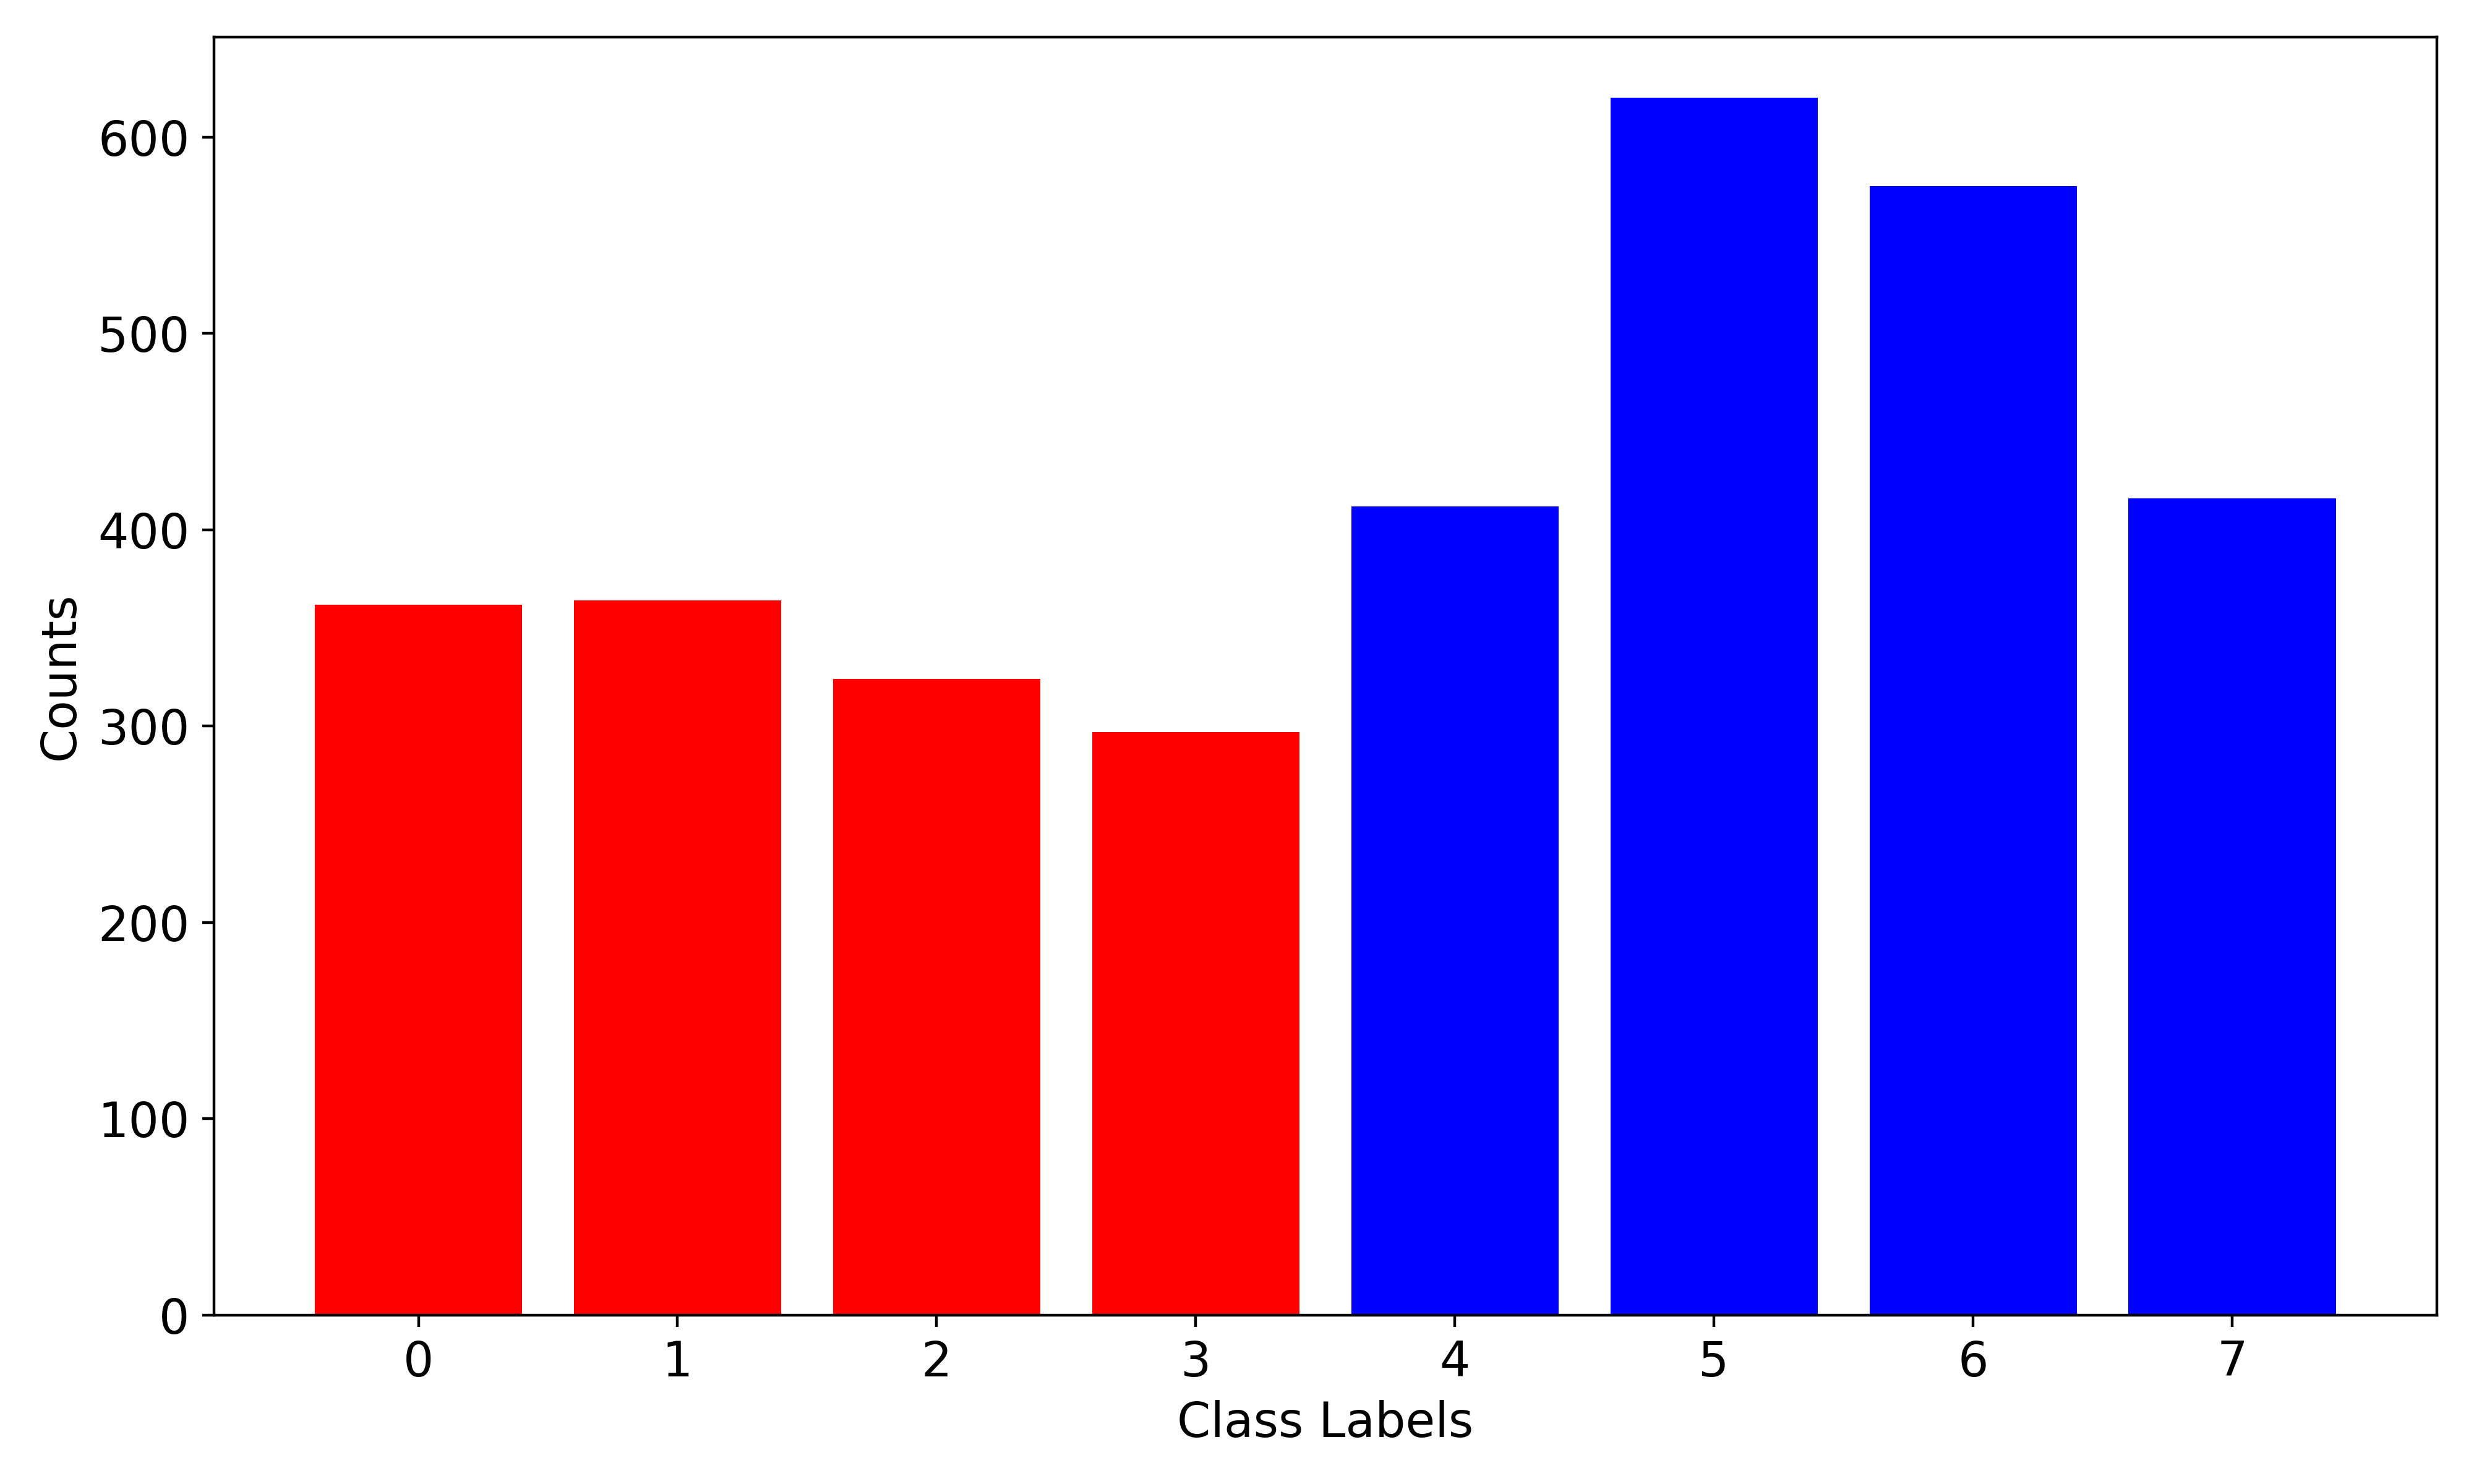
\includegraphics[width=0.9\textwidth]{Figures/Methods/ring_rls.png}
    \end{subfigure}
    \caption{Number of samples in each mode from RING dataset: Original RING(left), Vanilla Gen-RKM (middle) and Gen-RKM with RLS sampling (right).}
    \label{fig-ring-rkm}
\end{figure}

\begin{figure}[ht]
    \centering
    \begin{subfigure}{0.45\textwidth}
        \centering
        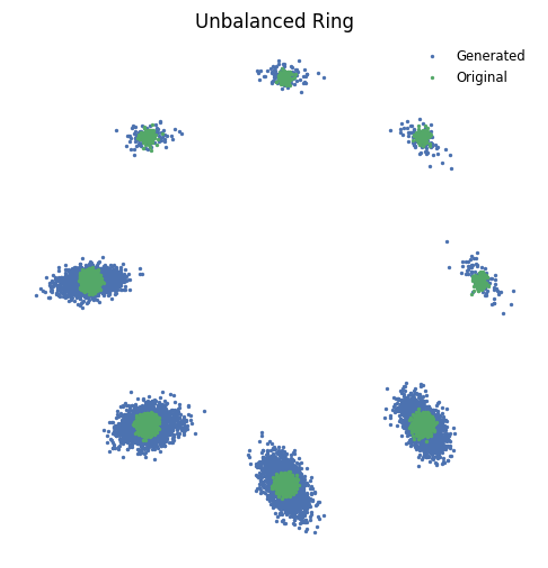
\includegraphics[width=0.8\textwidth]{Figures/Methods/2dring_rkm.png}
    \end{subfigure}
    \hfill
    \begin{subfigure}{0.45\textwidth}
        \centering
        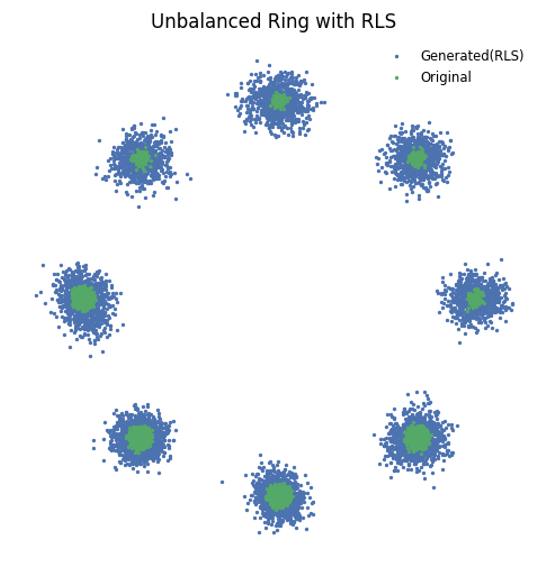
\includegraphics[width=0.8\textwidth]{Figures/Methods/2dring_rls.png}
    \end{subfigure}
    \hfill
    \begin{subfigure}{0.45\textwidth}
        \centering
        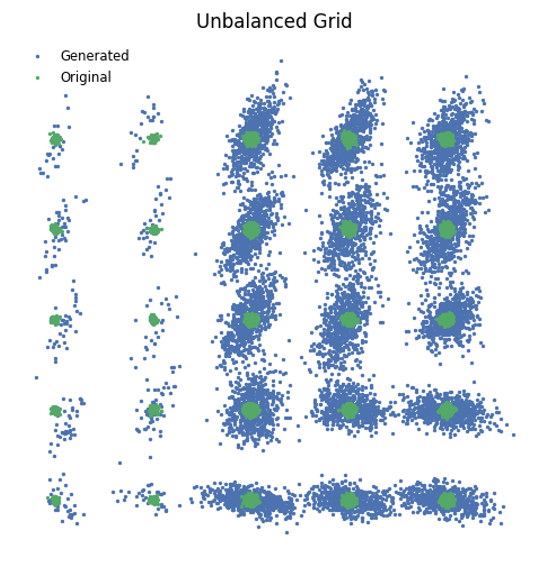
\includegraphics[width=0.8\textwidth]{Figures/Methods/2dgrid_rkm.png}
    \end{subfigure}
    \hfill
    \begin{subfigure}{0.45\textwidth}
        \centering
        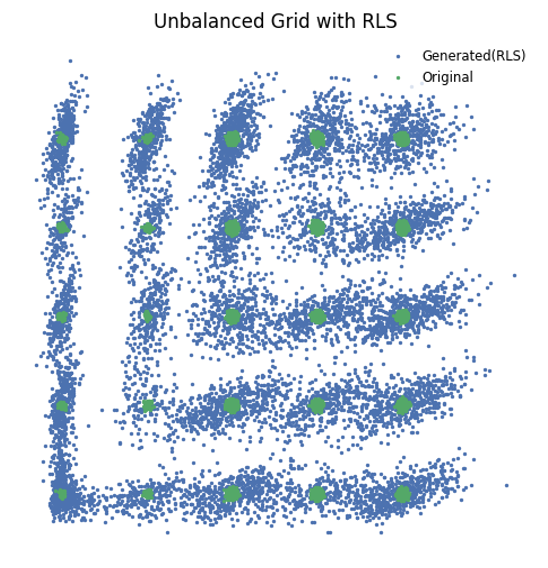
\includegraphics[width=0.8\textwidth]{Figures/Methods/2dgrid_rls.png}
    \end{subfigure}
    \caption{Visualizations of random generations on synthetic datasets: Vanilla Gen-RKM on RING (top left), Gen-RKM with RLS sampling on RING (top right), Vanilla Gen-RKM on GRID (down left) and Gen-RKM with RLS sampling on GRID (down right).}
    \label{2d-rkm-vis}
\end{figure}

\begin{table}[ht]
\centering
\begin{tabular}{@{}l*{4}{>{\centering\arraybackslash}p{2.5cm}}@{}}
\toprule
& \multicolumn{2}{c}{Ring with 8 modes} & \multicolumn{2}{c}{Grid with 25 modes} \\
\cmidrule(lr){2-3} \cmidrule(lr){4-5}
& Num modes & Minority mean & Num modes & Minority mean \\
\midrule
RKM      & 4.7(0.67) & 17.4(8.02) & 13.4(0.97) & 3.45(0.63) \\
RLS-RKM(shared)  & \textbf{7.7(0.48)} & 284.0(54.90) & 14.2(0.91) & \textbf{74.5(3.01)} \\
RLS-RKM(rbf) & 7.0(1.25) & \textbf{344.73(43.71)} & \textbf{20.02(1.75)} & 62.6(3.97) \\
\bottomrule
\end{tabular}
\caption{Results of experiments on 2D synthetic datasets (Experiments are replicated over 10 runs with random initialization).}
\label{tab-2d}
\end{table}


\FloatBarrier

\subsection{Unbalanced 012-MNIST}
\label{subsec-expr-ubMNIST012}
In this experiment, the performance of different weighted sampling schemes is studied on the unbalanced 012-MNIST dataset, which corresponds to a single minority mode scenario. Specifically, two RLS sampling variants with Gen-RKM are considered: RLSs computed based on an explicit feature map obtained from the last-to-next-layer of a pre-trained classifier (abbreviated as "RLS-RKM (class)"), and RLSs calculated from shared feature map with Gen-RKM (abbreviated as "RLS-RKM (shared)"), as described in Section \ref{subsec-methods-incor-rls-with-Genrkm}. In addition, weighted sampling built on isolation forest score (described in Section \ref{subsec-methods-islation-forest} and abbreviated as "Iforest RKM") is included. The baseline model in our experiment is Gen-RKM without any modifications but with the same network architecture and hyperparameter setting. In the evaluation process, the mode of each generated sample is identified by a well-trained MNIST classifier based on a ResNet18 architecture, which achieves 99.4\% accuracy on the test set. The results of calculated metrics are presented in Table \ref{expr-mnist012} where "Minority" refers to the number of generated samples classified as minority mode, and the distribution of numbers of generated samples under each mode is showcased in Figure \ref{fig-rls-gen-dist-ubmnist012}.  

It can be observed from Table \ref{expr-mnist012} that both RLS sampling and Iforest sampling could improve mode coverage and encourage more diverse generation under various imbalance ratio settings. More specifically, RLS-RKM (class) clearly outperforms all other methods in terms of both KL score and FID. Overall, This experiment demonstrates the immense effectiveness of RLS sampling with a pre-tained classifier as explicit feature map in single minority mode scenario. Samples from the minority group are generated more frequently as shown in Figure \ref{fig-gensamples-ubmnist012-rls}, thus a debiased generation is achieved.

\begin{table}[htb]
    \centering
    \begin{tabular}{ccccc}
\toprule
\makecell{Imbalance \\ ratio} & Model & Minority & KL score ($\downarrow$) & FID ($\downarrow$) \\
\midrule
\multirow{4}{*}{0.05} & RKM & 75 (±34) & 0.37 (±0.02) & 64.97 (±2.25) \\
& RLS-RKM (shared) & 410 (±60) & 0.32 (±0.02) & 74.09 (±3.39) \\
& RLS-RKM (class) & \textbf{1563} (±201) & \textbf{0.09} (±0.02) & \textbf{55.95} (±4.52) \\
& IforestRKM & 295 (±150) & 0.30 (±0.04) & 65.22 (±2.79) \\
\midrule
\multirow{4}{*}{0.10} & RKM & 135 (±76) & 0.35 (±0.03) & 65.04 (±1.74) \\
& RLS-RKM (shared) & 782 (±64) & 0.24 (±0.01) & 70.02 (±1.07) \\
& RLS-RKM (class) & \textbf{2259} (±144) & \textbf{0.03} (±0.01) & \textbf{55.42} (±6.33) \\
& IforestRKM & 863 (±180) & 0.18 (±0.03) & 59.63 (±3.74) \\
\midrule
\multirow{4}{*}{0.30} & RKM & 842 (±113) & 0.18 (±0.02) & 56.98 (±1.54) \\
& RLS-RKM (shared) & 2016 (±171) & 0.09 (±0.01) & 62.04 (±3.32) \\
& RLS-RKM (class) & \textbf{2868} (±77) & \textbf{0.01} (±0.00) & 51.95 (±3.60) \\
& IforestRKM & 2206 (±183) & 0.04 (±0.02) & \textbf{51.77} (±4.33) \\
\bottomrule
\end{tabular}
    \caption{Results of experiments on the unbalanced 012-MNIST dataset under different imbalance ratios. Experiments are replicated over 5 runs with random initializations. Means and standard deviations (enclosed in parentheses) for each metric are reported.}
    \label{expr-mnist012}
\end{table}
\begin{figure}[htb]
    \centering
    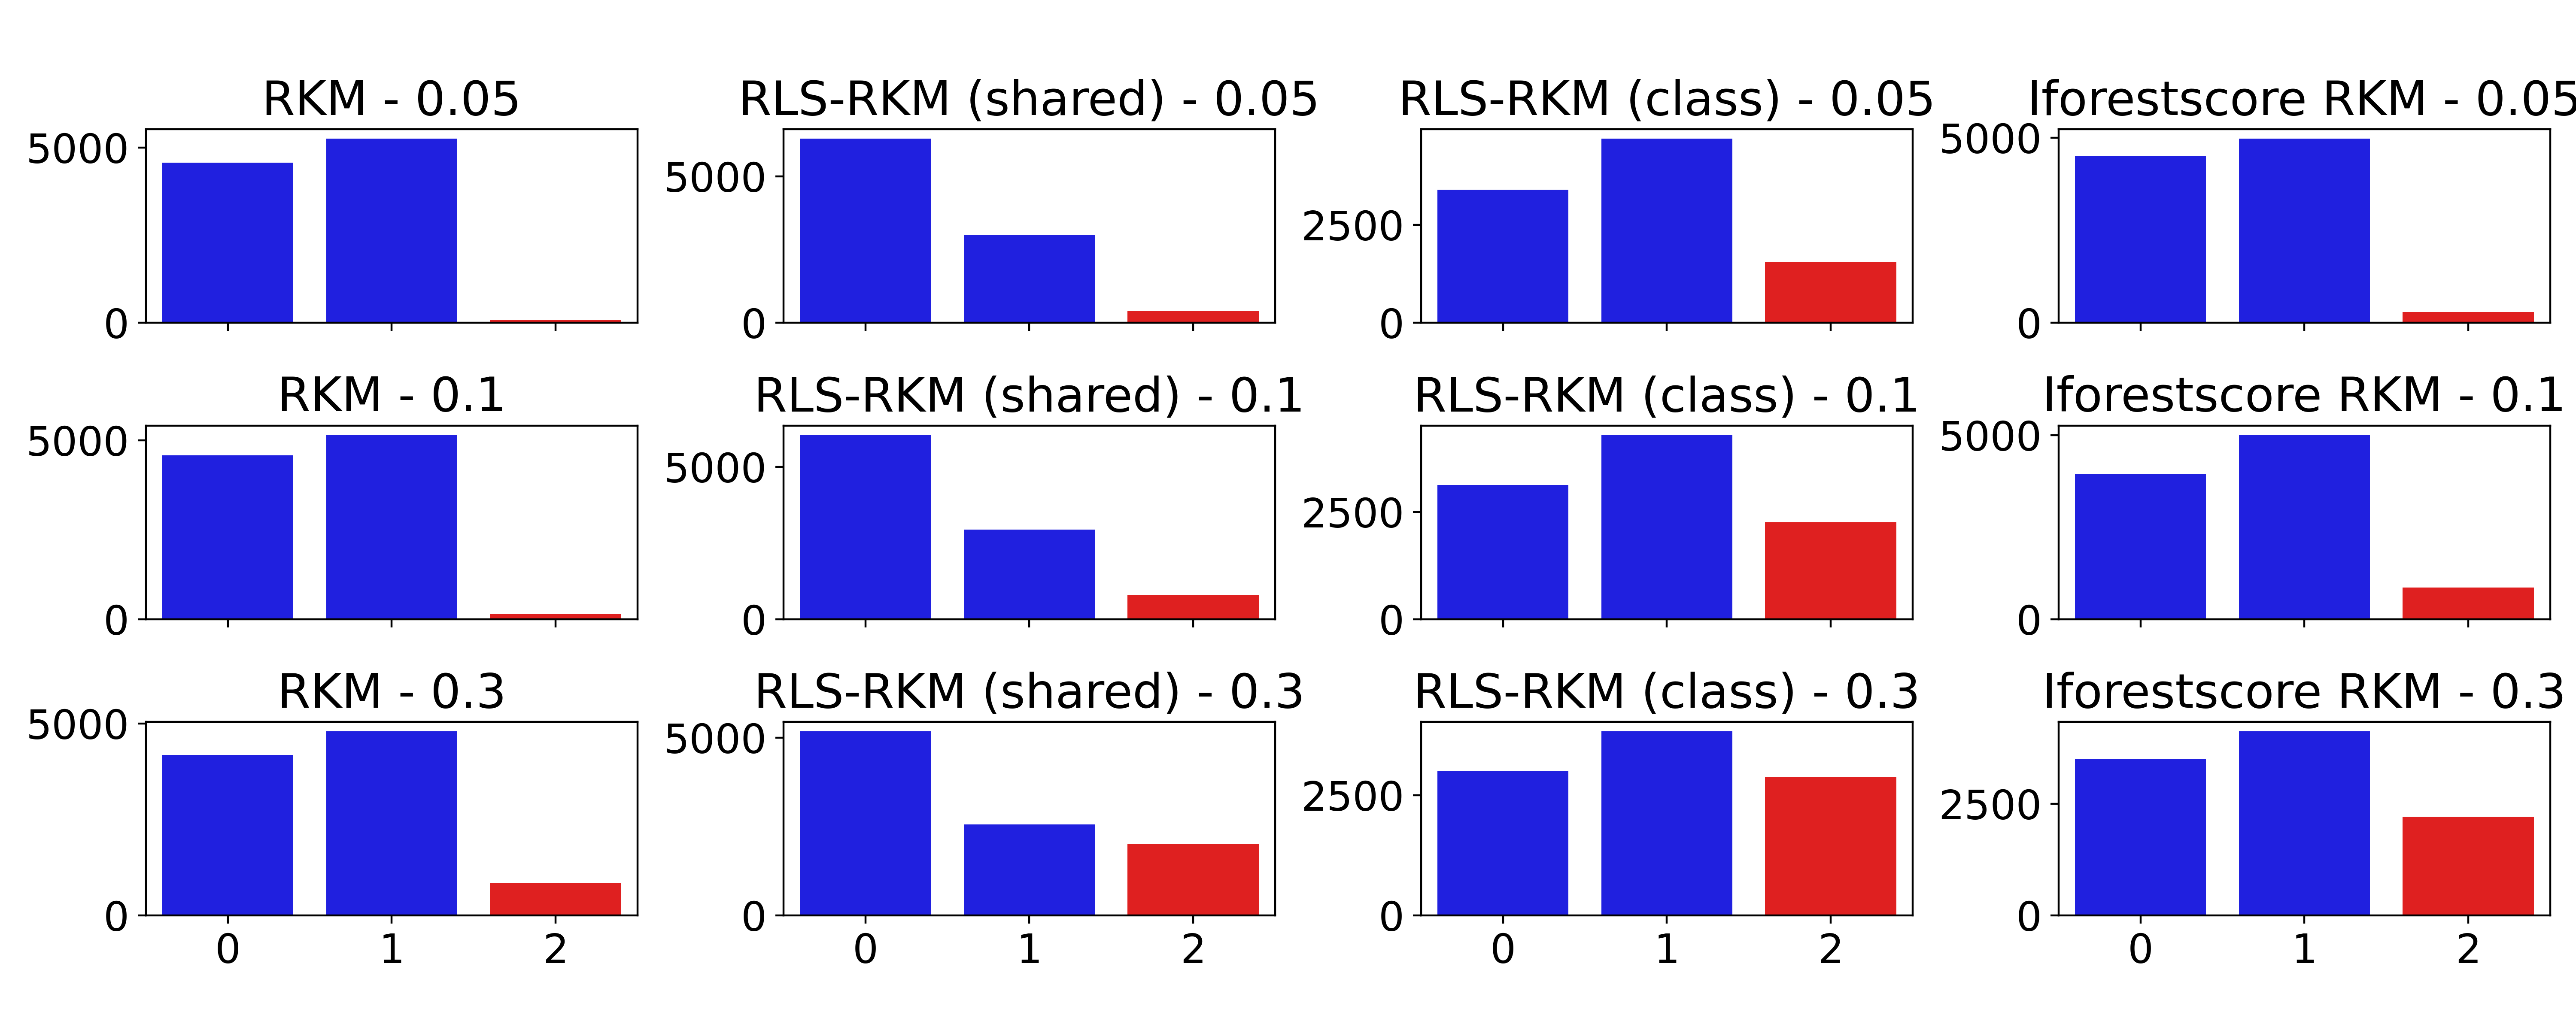
\includegraphics[width=0.9\linewidth]{Figures/Methods/expr-mnist012-gen-dist.png}
    \caption{Number of generated samples per mode from different RKM models on the unbalanced 012-MNIST dataset. Each row indicates that the dataset is generated with a specific balance ratio. Each column corresponds to a different model used. The minority mode in each figure is depicted in red color and, the majority modes are depicted in blue.}
    \label{fig-rls-gen-dist-ubmnist012}
\end{figure}

\subsection{Unbalanced MNIST}
\label{subsec-expr-ubMNIST}
It would also be meaningful to investigate how RLS sampling and Iforest sampling perform on a more challenging dataset, one that has multiple minority classes instead of just one. In the unbalanced MNIST dataset, half of the classes are minority classes, namely digits 0-4. Similarly, RLS-RKM (class) achieves best performance on KL score and FID compared with other approaches as observed from Table \ref{rls-expr-mnist}. Resampling schemes can more or less improve mode coverage in unbalanced data; however, when the imbalance ratio is very small (i.e., extremely unblanaced data), the improvement can be significantly diminished. If one looks at the distribution of generated labels in Figure \ref{fig-rls-gen-dist-ubmnist}, it is interesting to find that not all minority classes are oversampled when in RLS-RLM (class) and Iforest RKM. Instead, some particular minority classes might be downsampled. For example, minority classes such as digits 2,3, and 4 are generated even less frequently than before using RLS sampling or Iforest sampling, while only digits 0 and 1 are generated more frequently. This would ultimately result in a more unbalanced distribution of generated samples, as can be observed in the third and the fourth columns of Figure \ref{fig-rls-gen-dist-ubmnist}. Considering the sampling weights in both RLS (class) sampling and Iforest sampling are calculated based on embeddings extracted by a pre-trained classifier. Since this pre-trained classifier was not trained on this specific training dataset, it might fail to distinguish certain minority classes from others. The relatively low uniqueness results in a lower probability of being sampled. As for the RLS-RKM (shared), all minority classes are generally oversampled, but its ability to correct the imbalance is relatively weaker compared to other methods. To conclude, although weighted sampling schemes can more or less improve the diversity and quality of generation given unbalanced data with multiple minority modes, none of our methods could successfully captured all the underrepresented groups in the unbalanced MNIST dataset.
\begin{table}[ht]
    \centering
    \begin{tabular}{ccccc}
\toprule
\makecell{Imbalance \\ ratio} & Model & Minority mean & KL score ($\downarrow$) & FID ($\downarrow$) \\
\midrule
\multirow{4}{*}{0.05} & RKM & 113 (±13) & 0.49 (±0.02) & 39.19 (±1.17) \\
& RLS-RKM (shared) & 179 (±11) & 0.42 (±0.01) & 40.36 (±0.46) \\
& RLS-RKM (class) & \textbf{342} (±35) & \textbf{0.35} (±0.01) & \textbf{34.65} (±1.95) \\
& IforestRKM & 144 (±15) & 0.49 (±0.02) & 39.08 (±1.01) \\
\midrule
\multirow{4}{*}{0.10} & RKM & 185 (±11) & 0.40 (±0.01) & 38.89 (±0.18) \\
& RLS-RKM (shared) & 327 (±3) & \textbf{0.27} (±0.00) & 38.38 (±0.93) \\
& RLS-RKM (class) & \textbf{462} (±15) & \textbf{0.27} (±0.01) & \textbf{33.68} (±0.97) \\
& IforestRKM & 257 (±7) & 0.37 (±0.01) & 35.32 (±1.17) \\
\midrule
\multirow{4}{*}{0.30} & RKM & 478 (±14) & 0.15 (±0.01) & 34.09 (±1.28) \\
& RLS-RKM (shared) & 629 (±11) & \textbf{0.10} (±0.01) & 36.01 (±0.97) \\
& RLS-RKM (class) & \textbf{797} (±14) & 0.13 (±0.01) & \textbf{30.74} (±1.67) \\
& IforestRKM & 547 (±44) & 0.15 (±0.02) & 32.23 (±0.24) \\
\bottomrule
\end{tabular}
    \caption{Results of experiments on the unbalanced MNIST dataset under different imbalance ratios. Experiments are replicated over 3 runs with random initializations. Means and standard deviations (enclosed in parentheses) for each metric are reported. "Minority mean" refers to the average number of samples generated from each minority mode.
}
    \label{rls-expr-mnist}
\end{table}


\begin{figure}[ht]
    \centering
    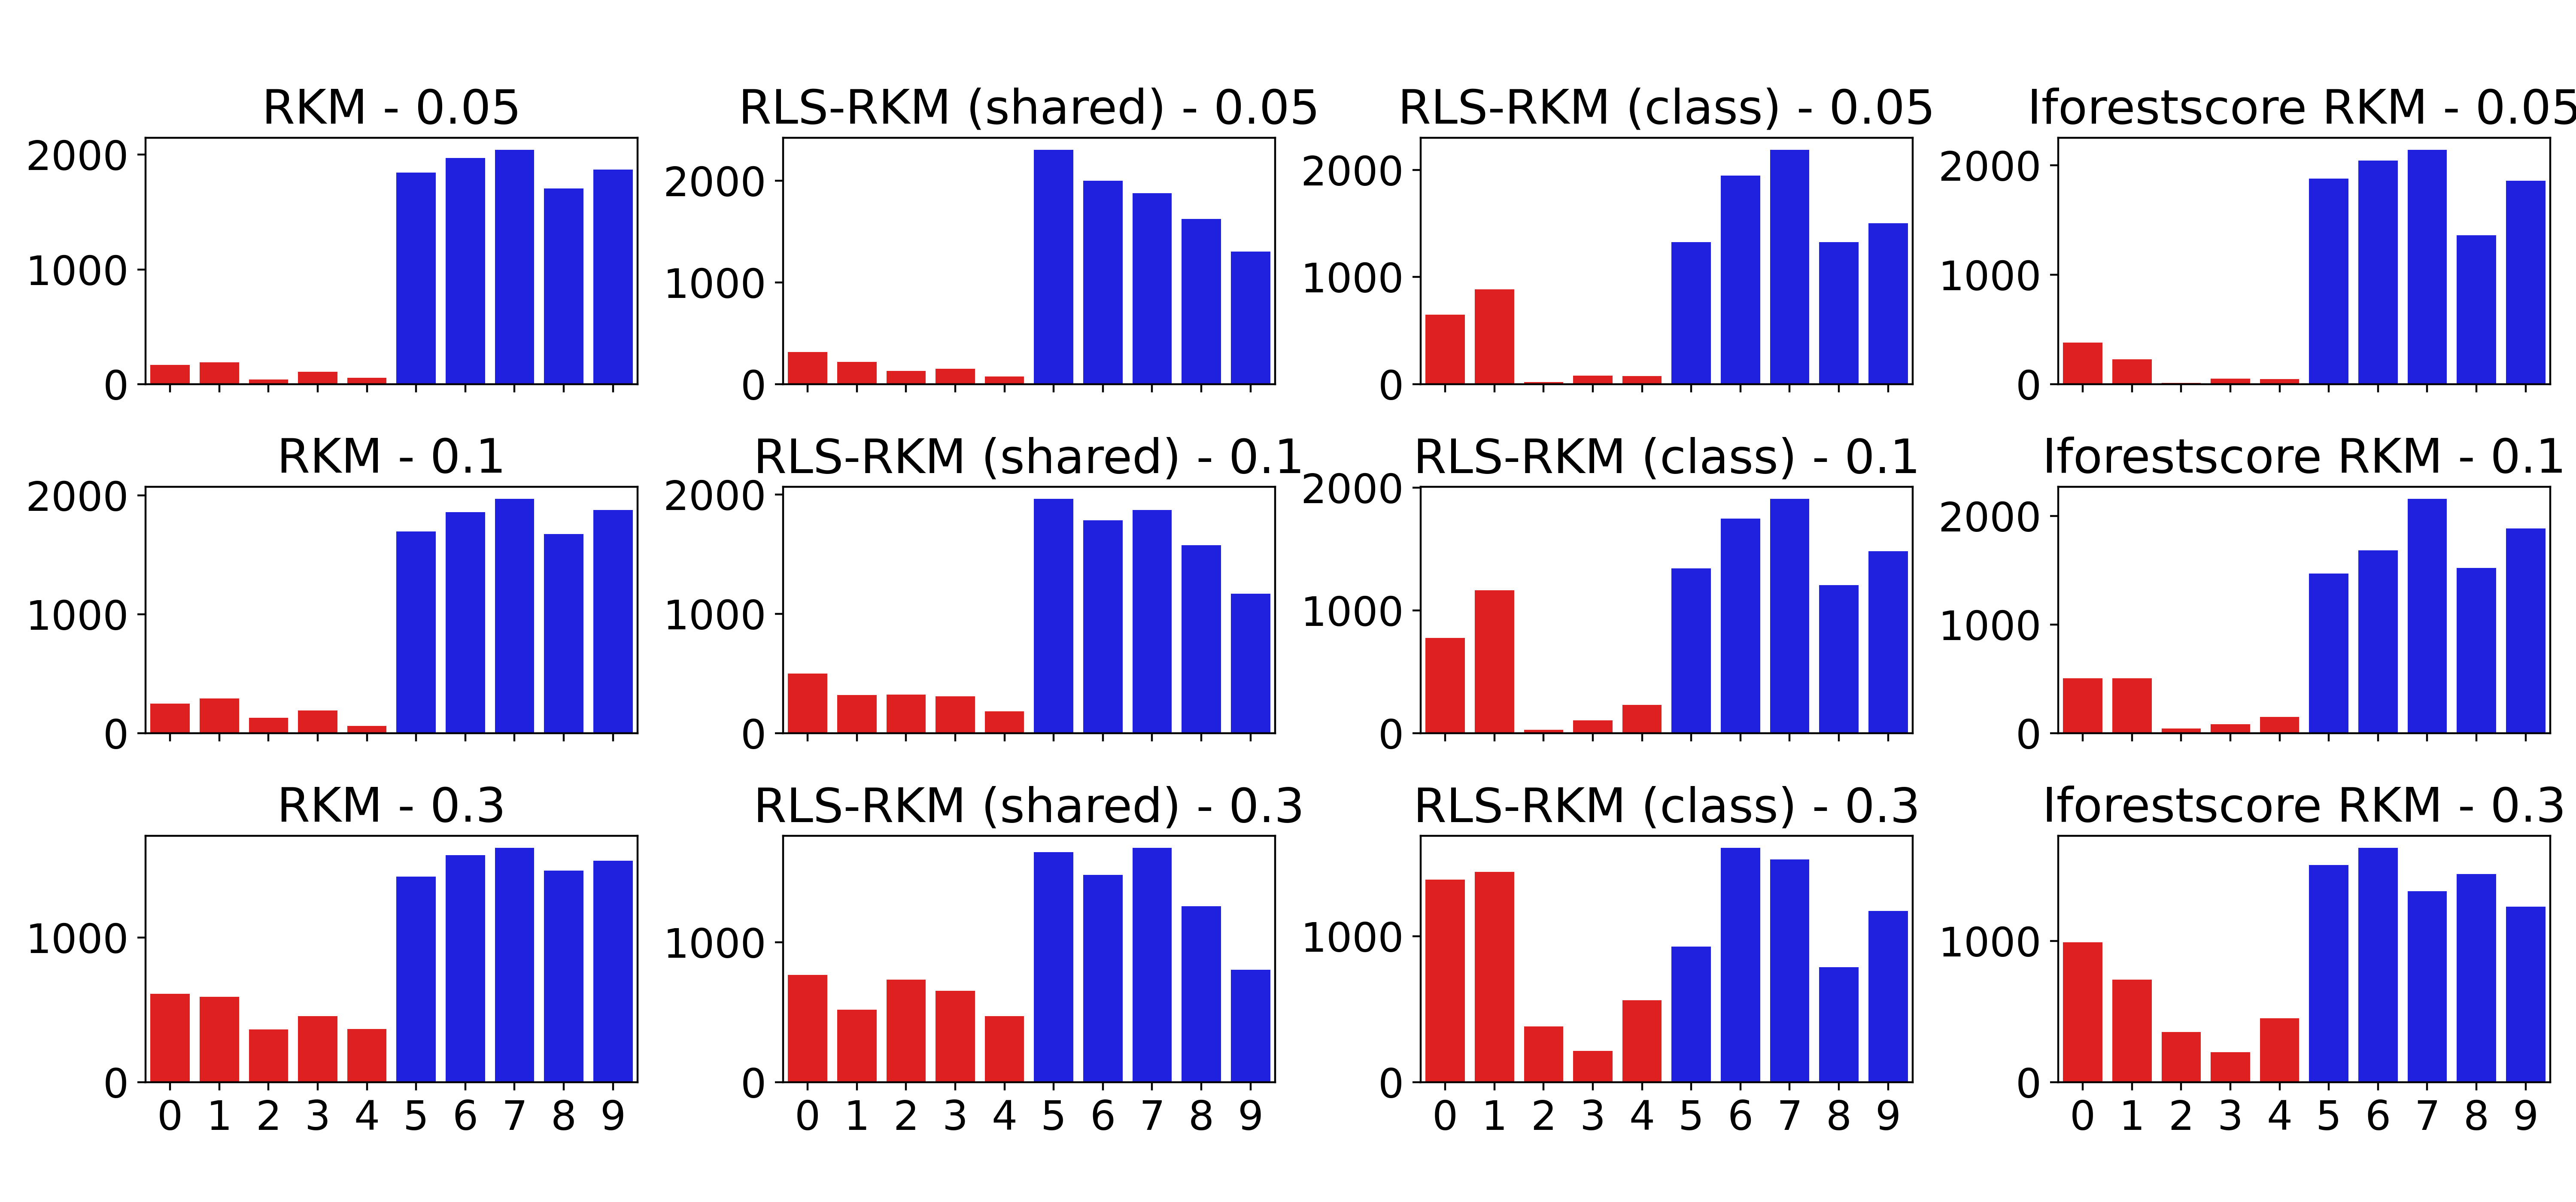
\includegraphics[width=0.9\linewidth]{Figures/Methods/expr-rls-mnist-gen-dist.png}
    \caption{Number of generated samples per mode from different RKM models on the unbalanced MNIST dataset.}
    \label{fig-rls-gen-dist-ubmnist}
\end{figure}


\subsection{Unbalanced Fashion MNIST}
\label{subsec-expr-Fashion}
Until now, experiments related to natural image datasets have only conducted on handwritten digits. In this section, we verify whether the use of RLS sampling and Iforest sampling in Gen-RKM could maintain similar performance on the Fashion MNIST dataset. The class of each generated sample is identified by a resnet18-type classifier which is trained up to 90.8\% accuracy on the test set. Unlike unbalanced MNIST, most of the categories in unbalanced Fashion MNIST are minority classes, whereas unbalanced MNIST has an equal number of minority and majority classes. The performance results of different sampling approaches are reported in Table \ref{tab-expr-fashion} and in Figure \ref{fig-rls-gen-dist-fashion}. Compared to the previous experiment, the performance of almost all methods is slightly better. Additionally, RLS-RKM (class) continues to outperform other methods, achieving the smallest FID and KL score on the unbalanced Fashion MNIST dataset.

\begin{table}[ht]
    \centering
    \begin{tabular}{ccccc}
\toprule
\makecell{Imbalance \\ ratio} & Model & Minority mean & KL score ($\downarrow$) & FID ($\downarrow$) \\
\midrule
\multirow{4}{*}{0.1} & RKM & 273 (±2) & 0.58 (±0.01) & 93.02 (±1.12) \\
& RLS-RKM (class) & \textbf{623} (±13) & \textbf{0.20} (±0.02) & \textbf{70.92} (±0.28) \\
& RLS-RKM (shared) & 437 (±2) & 0.38 (±0.02) & 80.98 (±2.35) \\
& Iforest RKM & 406 (±48) & 0.41 (±0.06) & 83.71 (±4.15) \\
\bottomrule
\end{tabular}
    \caption{Results of experiments on unbalanced Fashion MNIST dataset. Experiments are replicated over 3 runs with random initializations. Means and standard deviations (enclosed in parentheses) for each metric are reported. "Minority mean" refers to the average number of samples generated from each minority mode.}
    \label{tab-expr-fashion}
\end{table}
\begin{figure}[ht]
    \centering
    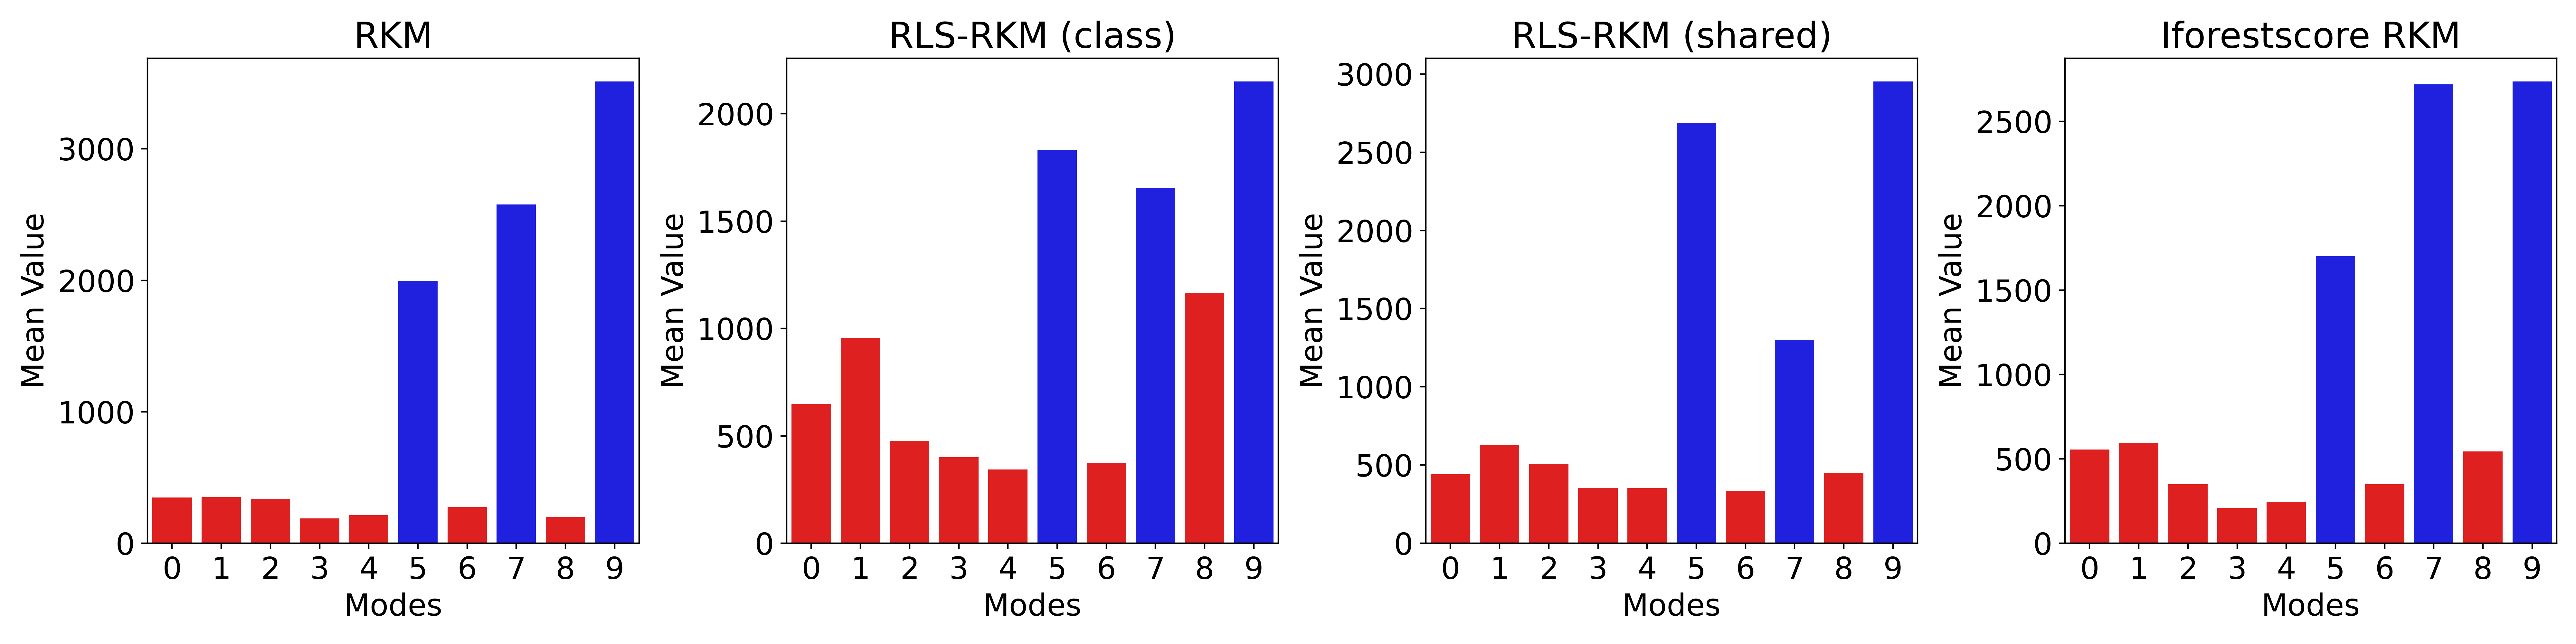
\includegraphics[width=0.9\linewidth]{Figures/Methods/expr-rls-fashion-gen-dist.png}
    \caption{Number of generated samples per mode from different RKM models on the unbalanced Fashion MNIST dataset.}
    \label{fig-rls-gen-dist-fashion}
\end{figure}

\subsection{Additional studies}
\label{subsec-additional-studies}

\begin{description}[leftmargin=0pt]
    \item[Ablation study on different pre-trained classifiers ] In the original work of RLS-GAN \cite{schreursLeverageScoreSampling2022}, the fixed explicit feature map for computing RLSs is derived from the last-to-the-next layer of an Inception-v3 network. However, the impact of different pre-trained classifiers was not compared. In this Section, an ablation study over the impact of various pre-trained classifiers in RLS-RKM (class) on the unbalanced 012-MNIST dataset is conducted. Specifically, the candidate pre-trained classifiers considered in our experiment include ResNet18\cite{heDeepResidualLearning2016}, ResNet34\cite{heDeepResidualLearning2016}, VGG16\cite{simonyanVeryDeepConvolutional2015}, AlexNet\cite{krizhevskyImageNetClassificationDeep2012}, and Inception-v3\cite{szegedyRethinkingInceptionArchitecture2016}. As shown in Table \ref{expr-different-classifiers}, we empirically observe that RLS sampling with pre-trained AlexNet as explicit feature map achieves the best performance across all evaluation metrics.

    \begin{table}[ht]
\centering
\begin{tabular}{lccccc}
\toprule
                     Classifier &      Mode 1 &      Mode 2 &      \textbf{Mode 3} &       KL score($\downarrow$) &           FID($\downarrow$) \\
\midrule
     Alexnet\cite{krizhevskyImageNetClassificationDeep2012} & 3219 (±218) & 4183 (±125) & \textbf{2283} (±299) & \textbf{0.03} (±0.02) & \textbf{52.02} (±4.32) \\
Inception\_v3\cite{szegedyRethinkingInceptionArchitecture2016} & 3998 (±242) & 4496 (±122) & 1206 (±278) & 0.12 (±0.04) &   60.4 (±4.4) \\
    Resnet18\cite{heDeepResidualLearning2016} & 3706 (±188) &  4231 (±94) & 1738 (±286) & 0.06 (±0.02) &  57.31 (±3.7) \\
    Resnet34\cite{heDeepResidualLearning2016} &  3328 (±59) & 4945 (±177) & 1486 (±231) &  0.1 (±0.02) &  55.34 (±3.0) \\
       vgg16\cite{simonyanVeryDeepConvolutional2015} &  3765 (±77) & 4538 (±183) & 1446 (±130) & 0.09 (±0.02) & 59.53 (±2.11) \\
\bottomrule
\end{tabular}
\caption{Ablation study over the impact of different pre-trained classifiers on the performance of RLS-RKM (class) on the unbalanced 012-MNIST dataset. Minority mode is highlighted in bold, with the imbalance ratio set to 0.1. The results are averaged over 5 runs of replicated experiments.}
\label{expr-different-classifiers}
\end{table}

    \item[Effect of weighted sampling on latent space in Gen-RKM ] It is also non-trivial to analyze the impact of the use of weighted sampling schemes during training in Gen-RKM on its corresponding latent space. The visualizations of the latent spaces obtained from the standard training process and that from the RLS sampling-adapted training process are shown in Figure \ref{fig-rls-latent-space-vis}. It is evident that the latent variables corresponding to the minority classes are also augmented in the latent space, and a re-balancing effect is significant. This ensures that the fitted GMM would not overlook these underrepresented groups, thereby reducing the unwanted bias towards majority modes that arise from unbalanced training data in generation. A more diverse and fair generation can thus be obtained in this spirit.

    \indent However, augmenting minority classes via oversampling techniques also has some drawbacks. Since correction for imbalance is achieved by oversampling the minority classes, the resampled training data will inevitably contain some duplicate instances. During the KPCA operation, these duplicate data will still yield redundant hidden representations in the latent space, as displayed in the right side of Figure \ref{fig-rls-latent-space-vis}. The negative effects are in two-fold. First, the smoothness and the continuity of the latent space are no longer guaranteed, where interpolation between latent points could be problematic. Second, the presence of duplicate latent points might cause the GMM to be overfitted, where duplicate points are assigned higher probabilities. That would increase the risk of data-copying (i.e., directly replicating certain training samples in generation) in the generative models, which has been shown as orthogonal to the problem of mode collapse \cite{bhattacharjeeDatacopyingGenerativeModels2023}.  

    \begin{figure}[ht]
    \centering
    \begin{subfigure}{0.45\textwidth}
        \centering
        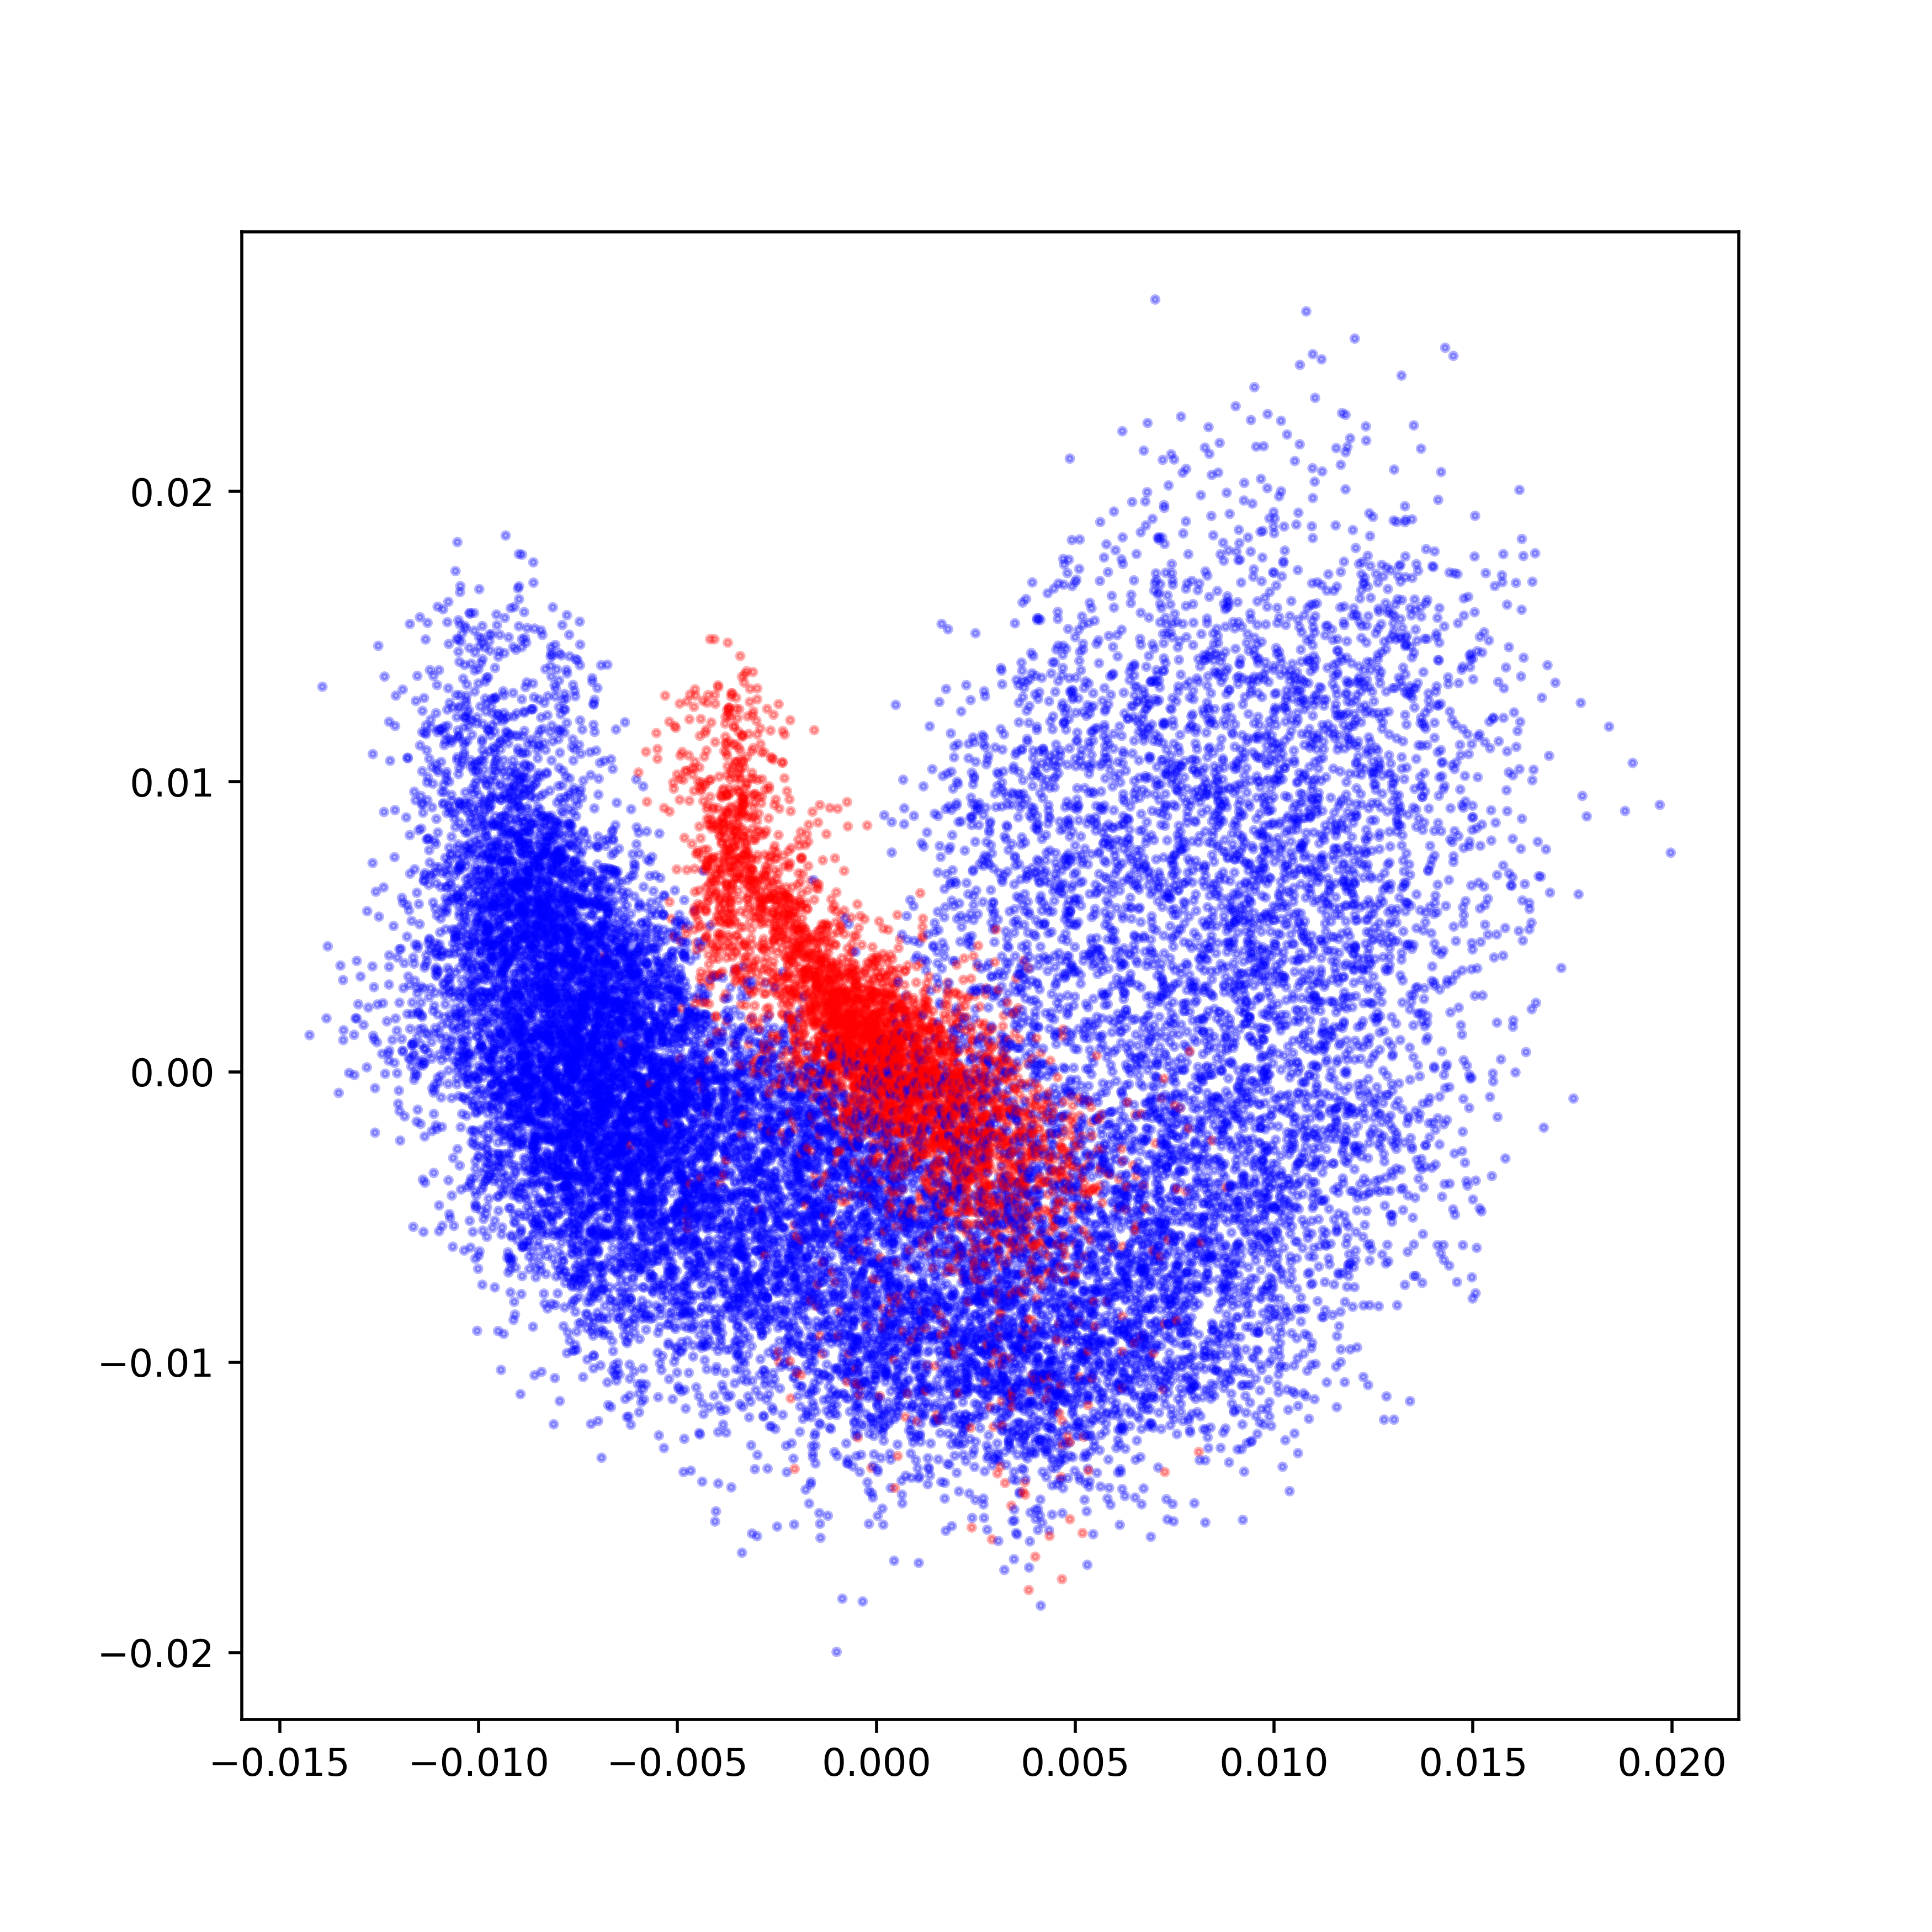
\includegraphics[width=0.9\textwidth]{Figures/Methods/ubFashion-latentspace-vis.png}
    \end{subfigure}
    \hfill
    \begin{subfigure}{0.45\textwidth}
        \centering
        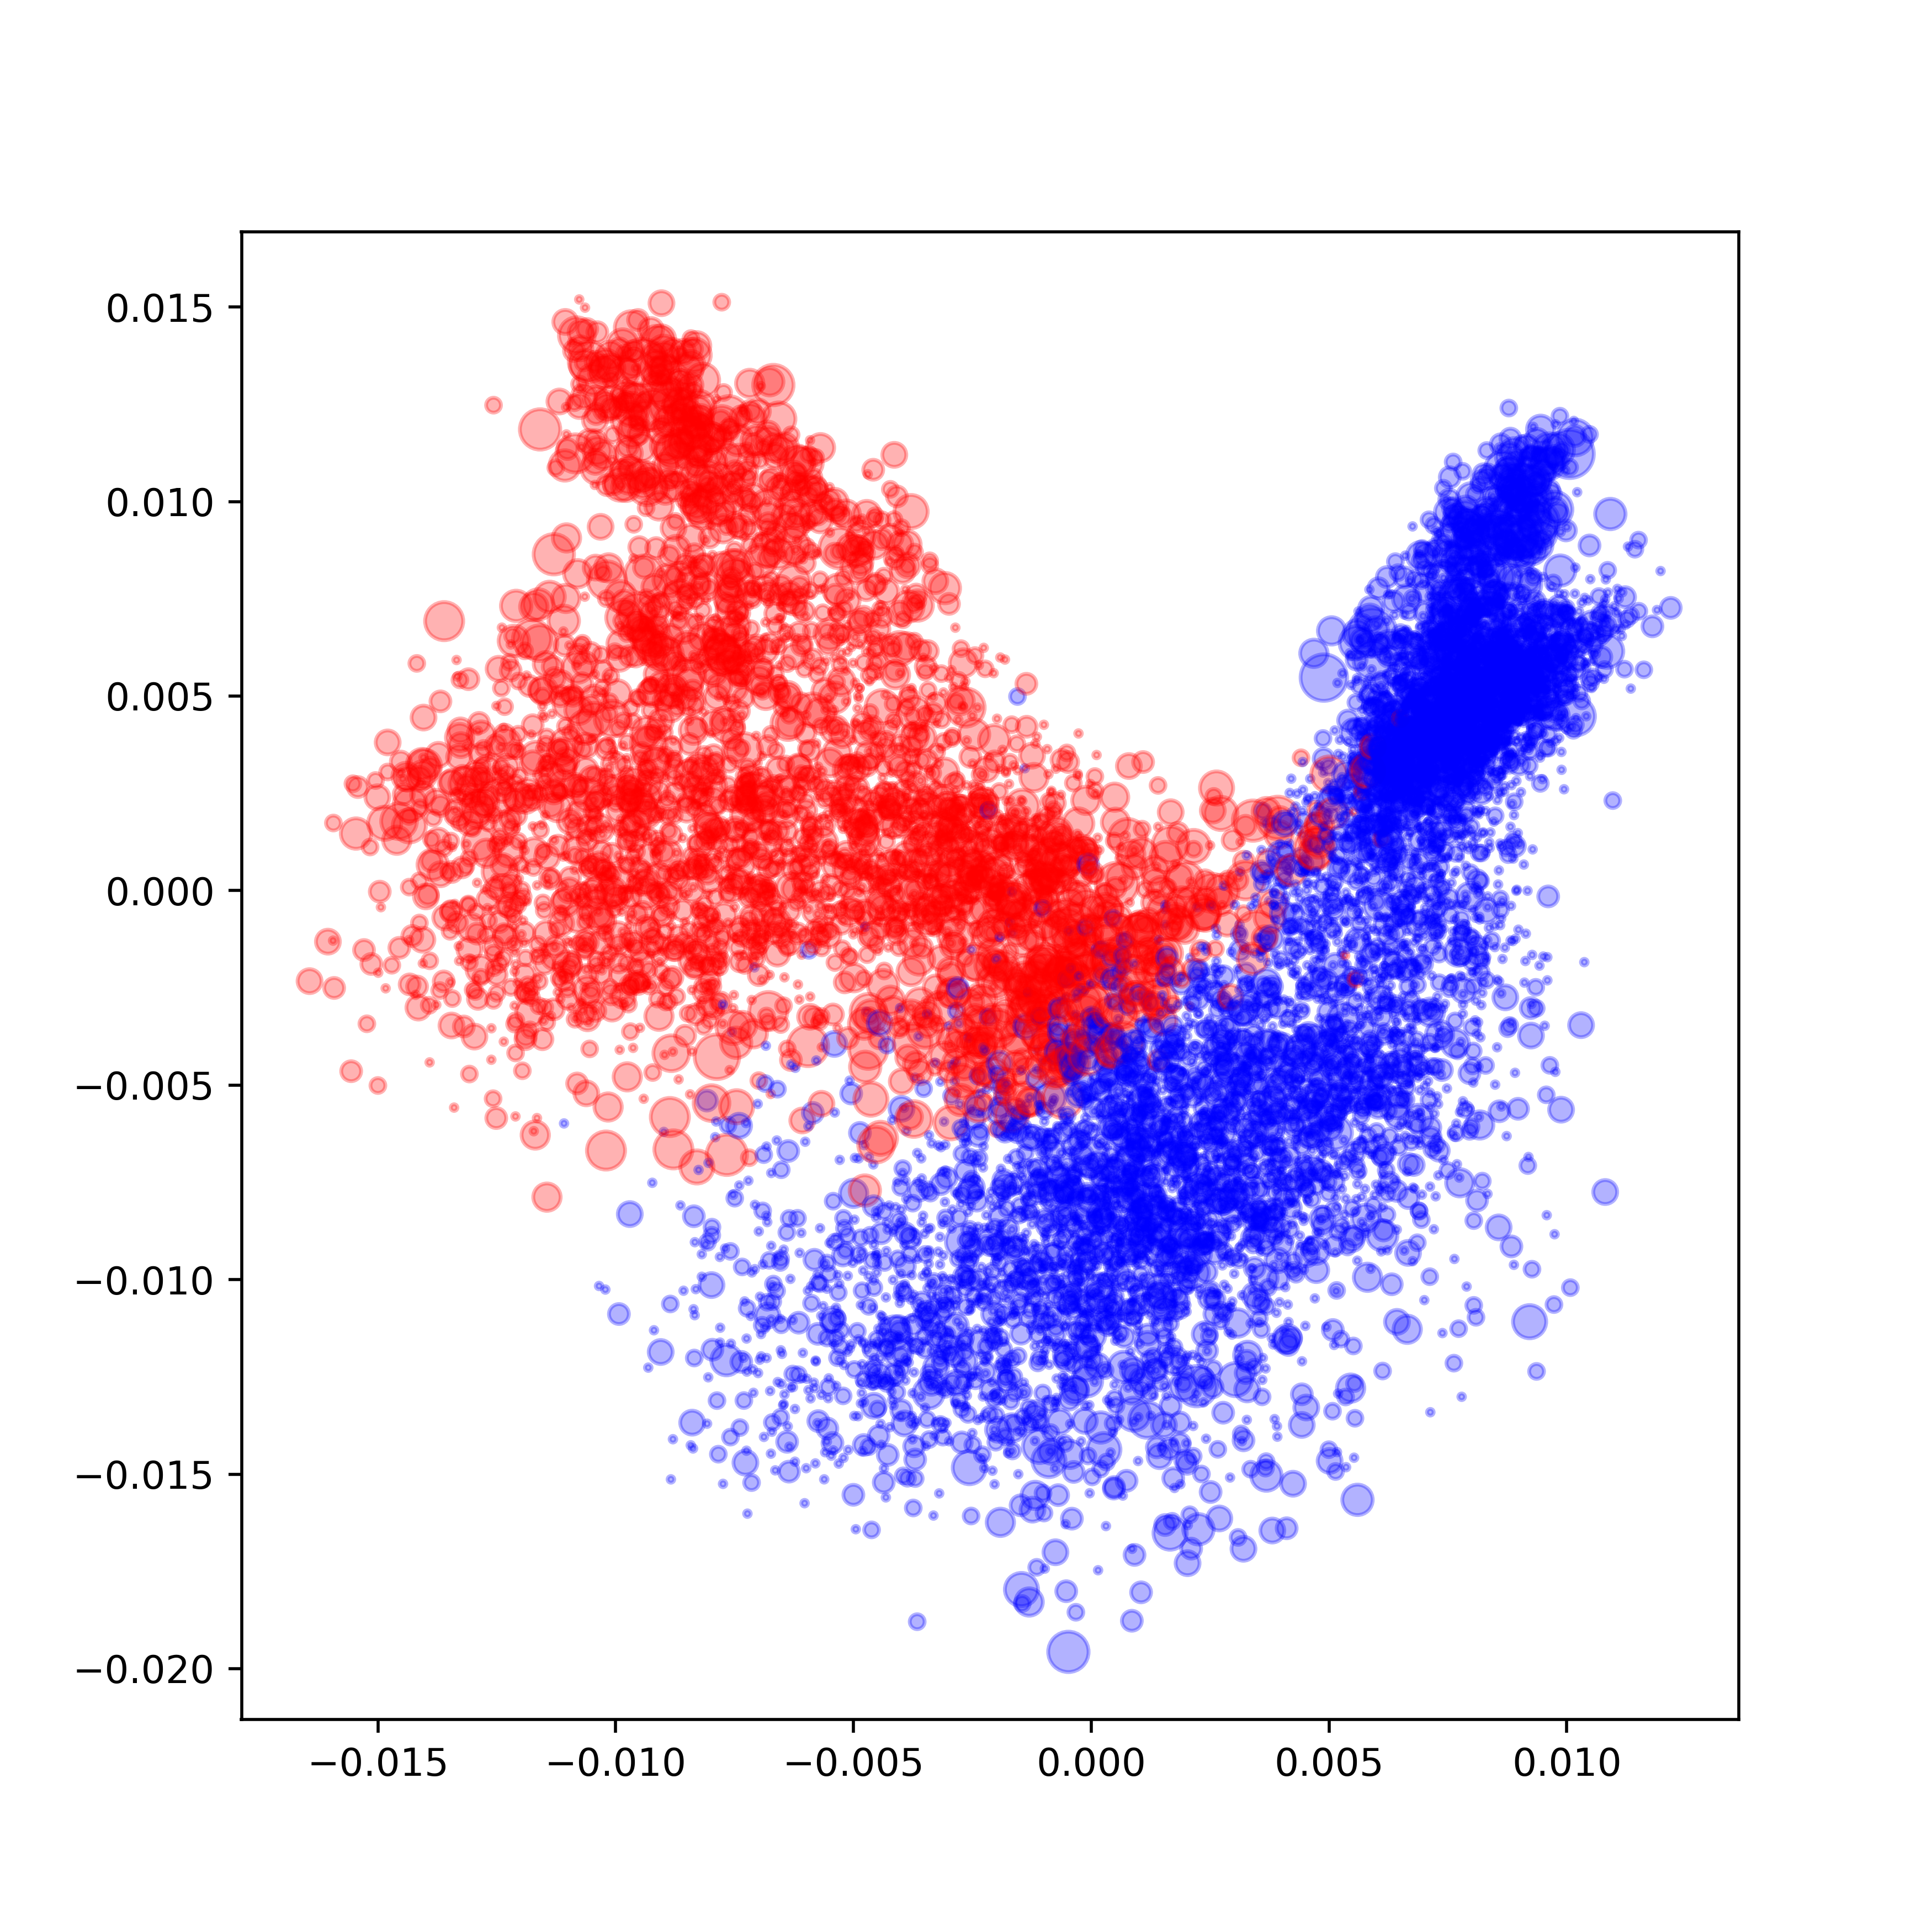
\includegraphics[width=0.9\textwidth]{Figures/Methods/RLS-ubFashion-latentspace-vis.png}
    \end{subfigure}
    \caption{Visualizations of the latent spaces of two Gen-RKMs trained on the unbalanced Fashion MNIST dataset (imbalance ratio is 0.1). Only the first two principal components in the latent spaces are displayed. The left figure is developed based on a vanilla Gen-RKM, whereas Gen-RKM in the right figure is trained with the RLS sampling (class) manner. Latent representations of minority modes are colored as red, while those of the majority classes are in blue. Note that the size of each point in the right figure indicates the frequency of being oversampled.}
    \label{fig-rls-latent-space-vis}
\end{figure}

    \item[Comparison to VAE and RLS-VAE ] A qualitative comparison is made in this section between the proposed methods and the standard VAE model. We also include the RLS sampling adapted version of VAE in this experiment to evaluate the effectiveness of RLS sampling across different model settings. The results are displayed in Table \ref{expr-comparison-vae}. Note that the same encoder and decoder architecture, along with the hyperparameter settings as outlined in Section \ref{subsec-setup-hyperparameter} is employed in VAE for a fair comparison. We observe empirically that both FID scores and KL scores are better with the Gen-RKM setting. In addition, the implementation of RLS sampling with a pre-trained classifier as feature map could significantly improve the mode coverage and capturing in both the Gen-RKM and VAE models. However, the use of RLS sampling in VAE could possibly lead to a lower FID score, indicating a poorer generation quality. 
    \begin{table}[ht]
\centering
\begin{tabular}{lcccccc}
\toprule
Model Name & Mode 1 & Mode 2 & \textbf{Mode 3} & KL Score($\downarrow$) & FID($\downarrow$) \\
\midrule
RKM & 4573(±44) & 5138(±90) & 165(±71) & 0.33(±0.02) & 61.60(±1.69) \\
RLS-RKM & 3153(±72) & 4280(±40) & \textbf{2276}(±113) & \textbf{0.03}(±0.00) & \textbf{56.65}(±1.39) \\
RLS-VAE & 3000(±78) & 4955(±198) & 1621(±262) & 0.10(±0.03) & 79.17(±2.70) \\
VAE & 4216(±101) & 5409(±154) & 176(±14) & 0.34(±0.01) & 76.39(±1.42) \\
\bottomrule
\end{tabular}
\caption{Results of comparison to VAE and RLS-VAE on the unbalanced 012-MNIST dataset with imbalance ratio 0.1. RLSs are computed by explicit feature map based on a pre-trained classifier.}
\label{expr-comparison-vae}
\end{table}

    \item[Timings of different sampling schemes ] The training times of Gen-RKM adapted with the proposed sampling schemes are reported in Table \ref{tab-sampling-training-time}. One can observe that the implementations of both RLS sampling and Iforest sampling in Gen-RKM are more computationally expensive compared to the standard training process. Among these,  RLS-RKM (shared) requires the longest training time due to the need for updating RLSs in each iteration. 
    \begin{table}[ht]
\centering
\begin{tabular}{lccc}
\toprule
{} &   Fashion &     MNIST & 012-MNIST \\
\cmidrule(lr){2-2} \cmidrule(lr){3-3} \cmidrule(lr){4-4}
Number of samples & 22200   & 32467 & 13261 \\
\midrule
Iforest RKM &  391(±18) &  721(±44) &  158(±2) \\
RKM              &   233(±5) &   326(±4) &   91(±0) \\
RLS-RKM (class)  &  418(±19) &  737(±13) &  156(±1) \\
RLS-RKM (shared) &   450(±7) &  1029(±3) &  165(±5) \\
\bottomrule
\end{tabular}
\caption{Training times in seconds (averaged over 3 runs) of different weighted sampling implementations in Gen-RKM. For the unbalanced 012-MNIST, the maximum epoch number is set to 100, while the maximum epoch number in unbalanced MNIST and Fashion MNIST is 150. The batch size is uniformly set to 328 across all cases. All experiments are conducted using a single NVIDIA GeForce RTX 3080 GPU (12GB).}
\label{tab-sampling-training-time}
\end{table}


    \item[Significance of mini-batch sampling and final step resampling ] Recall that in the RLS sampling adapted Gen-RKM, two key modifications based on weighted sampling are introduced during the training phase. Firstly, each mini-batch in every iteration is sampled with replacement according to the probability determined by the normalized RLSs. Secondly, the final computation step in Gen-RKM is performed on the full dataset, which has been resampled based on these RLSs. It is interesting to investigate how the performance of RLS-RKM becomes if we remove one of the above modifications in the algorithm. To conduct this ablation study, two simplified versions of RLS-RKM are considered as follows.
    \begin{itemize}
        \item \textbf{RLS-RKM (batch): }Only mini-batch sampling is based on RLSs, while the final computation step remains unmodified (i.e., performing KPCA on the original, unbalanced dataset). 

        \item \textbf{RLS-RKM (final): }Only the final computation step uses the resampled full dataset, while each mini-batch is uniformly sampled during the training phase, as usual.
    \end{itemize}
    The performance results of these two simplified versions of RLS-RKM are presented in Table \ref{expr-final-sample-or-mini-batch}. For RLS-RKM (batch), the performance shows almost no change compared to the vanilla RKM. This is not surprising, because the minority modes are not augmented in the latent space without the final resampling step, which inevitably makes it fail to generate more samples from the minority classes. As for RLS-RKM (final), a slight improvement on the mode coverage can be observed compared to vanilla RKM, but since the encoder and decoder parameters are not exactly trained on the resampled data, the quality of the final generation is actually worse than that of vanilla RKM. In conclusion, this ablation study demonstrates that the modifications on both mini-batch sampling and the final computation step are crucial to the effectiveness of the RLS-RKM algorithm.
    \begin{table}[ht]
\centering
\begin{tabular}{lcccccc}
\toprule
Model Name & Mode 1 & Mode 2 & \textbf{Mode 3} & KL score($\downarrow$) & FID($\downarrow$) \\
\midrule
RKM & 4623(±106) & 5185(±62) & 85(±46) & 0.36(±0.02) & 64.17(±0.28) \\
RLS-RKM & 3363(±196) & 4771(±162) & \textbf{1558}(±145) & \textbf{0.09}(±0.01) & \textbf{53.22}(±2.93) \\
RLS-RKM (batch) & 4496(±47) & 5249(±67) & 166(±17) & 0.34(±0.01) & 62.68(±2.91) \\
RLS-RKM (final) & 3759(±156) & 5111(±132) & 679(±186) & 0.21(±0.03) & 67.11(±6.06) \\
\bottomrule
\end{tabular}
\caption{Ablation study over the significance of mini-batch sampling and final step resampling in RLS-RKM. This experiment is conducted on the unbalanced 012-MNIST dataset with imbalance ratio of 0.05. RLSs are computed by an explicit feature map based on a pre-trained classifier.}
\label{expr-final-sample-or-mini-batch}
\end{table}
\end{description}


\section{Summary and discussion}
\label{sec-expr-summary}
This experiment chapter focuses on evaluating the effectiveness of different weighted sampling schemes implemented during the training of Gen-RKM on unbalanced datasets. Specifically, we conduct different experiments tailored to both supervised and unsupervised scenarios.

For the supervised setting, we assess the applicability of Gen-RKM adapted with inverse frequency sampling on the unbalanced MNIST and Fashion MNIST datasets. We then extend its use to conditional generation in the context of unbalanced data. From the results, we can conclude that
\begin{itemize}[label={--}]
\item A notable improvement in the diversity of generation can be observed when applying inverse frequency sampling. All minority modes can be successfully captured, and the distribution of generated samples becomes more uniform and balanced.
\item Unbalanced data may impact the effectiveness of conditional generation in Gen-RKM, leading to potentially blurred or incorrect results when generating samples conditioned on certain minority modes. This problem can be resolved by conditional generation based on a Gen-RKM trained with the inverse sampling manner, resulting in improved generation quality.

\item The limitation of inverse frequency sampling is quite evident. Since the sampling weights are determined by the inverse of class frequencies, it requires the knowledge of labels. Consequently, the applications of inverse frequency sampling are relatively limited in practice, as label information is often scarce in real-world scenarios.
\end{itemize}

More delicate experiments are carried out under the unsupervised setting to study the effectiveness of different RLS sampling schemes. Additionally, We also include Iforest sampling as an extension approach to basic RLS sampling. The used datasets vary from synthetic datasets to real-world image datasets. According to the results, the following findings can be concluded:
\begin{itemize}[label={--}]
    \item For the 2D synthetic dataset, we observe that RLS sampling is effective in preventing mode collapse and improving diversity in generation. However, for more complex datasets with a larger number of modes, such as the 2D grid, some minority modes may not be successfully captured.
    \item Regarding the unbalanced 012-MNIST dataset where there is only one minority mode, RLS sampling with a pre-trained classifier as the explicit feature map could significantly improve both mode coverage and generation quality under different imbalance ratios.
    \item A similar observation is made with the unbalanced MNIST and unbalanced Fashion MNIST datasets, where RLS-RKM (class) consistently outperforms other methods in terms of lower KL score and FID. However, there is a higher chance for the occurrence of mode missing due to the increasing number of minority modes in the datasets.
    \item A addition comparison to vanilla VAE and RLS-VAE is also conducted. The results indicate that using RLS sampling with VAE leads to a slightly lower FID score, suggesting a decrease in generation quality, despite great improvement in the aspect of mode coverage. Compared to Gen-RKM, the effect of RLS sampling on VAE is less pronounced.
\end{itemize}
Additionally, some drawbacks of RLS sampling can be identified from the above experiments and a series of additional studies.
\begin{itemize}[label={--}]
    \item RLS sampling is particularly dependent on the choice of feature map, which means that if the feature map fails to effectively extract information from the unbalanced data (i.e., it cannot distinguish well between minority modes and majority modes), the performance of RLS sampling could be rather poor.
    \item RLS sampling is rather computationally intensive, especially when using a shared feature map with Gen-RKM. Training could become significantly slower because the RLSs need to be recalculated in each iteration.
    \item The underlying mechanism behind RLS sampling (or possibly other weighted sampling schemes) leading to a more diverse generation in Gen-RKM is that minority modes in the latent space are also augmented via oversampling. However, this would cause the GMM to overfit, particularly on some repeated latent points, resulting in the generated samples that are very close to the true training samples. The risk of data copying in generation thus increases.
\end{itemize}

Overall, our experiments show that weighted sampling schemes like inverse frequency sampling and RLS sampling could more or less reduce the problem of mode collapse in Gen-RKM when facing unbalanced training data, leading to a more diverse and fair generation. Nevertheless, some limitations have been discovered, including the need for full label information in inverse frequency sampling, higher computational demands, the risk of data memorization, and reliance on feature maps in RLS sampling, which also suggest potential directions for future research.


% \begin{figure}[H]
%     \centering
%     \begin{subfigure}{0.45\textwidth}
%         \centering
%         \includegraphics[width=\textwidth]{Figures/Methods/rkm-fashion-gensamples-highlighted-minorities.png}
%     \end{subfigure}
%     \hfill
%     \begin{subfigure}{0.45\textwidth}
%         \centering
%         \includegraphics[width=\textwidth]{Figures/Methods/RLS-fashion-gensamples-highlighted-minorities.png}
%     \end{subfigure}
%     \caption{Generated images from unbalanced Fashion MNIST dataset by vanilla RKM (left) and RLS sampling adapted RKM (right). Feature map in RLS sampling is implemented by a pretrained classifier. Images are highlighted by a red border if classified as minority modes.}
%     \label{fig-gensamples-fashion-rls}
% \end{figure}


% \begin{figure}[H]
%     \centering
%     \begin{subfigure}{0.45\textwidth}
%         \centering
%         \includegraphics[width=\textwidth]{Figures/Methods/rkm-mnist012-gensamples-highlighted-minorities.png}
%     \end{subfigure}
%     \hfill
%     \begin{subfigure}{0.45\textwidth}
%         \centering
%         \includegraphics[width=\textwidth]{Figures/Methods/RLS-mnist012-gensamples-highlighted-minorities.png}
%     \end{subfigure}
%     \caption{Generated images from unbalanced 012-MNIST dataset by vanilla RKM (left) and RLS sampling adapted RKM (right). Feature map in RLS sampling is implemented by a pretrained classifier. Images are highlighted by a red border if classified as minority modes.}
%     \label{fig-gensamples-fashion-rls}
% \end{figure}

% \begin{figure}[H]
%     \centering
%     \begin{subfigure}{0.45\textwidth}
%         \centering
%         \includegraphics[width=\textwidth]{Figures/Methods/rkm-mnist-gensamples-highlighted-minorities.png}
%     \end{subfigure}
%     \hfill
%     \begin{subfigure}{0.45\textwidth}
%         \centering
%         \includegraphics[width=\textwidth]{Figures/Methods/RLS-mnist-gensamples-highlighted-minorities.png}
%     \end{subfigure}
%     \caption{Generated images from unbalanced MNIST dataset by vanilla RKM (left) and RLS sampling adapted RKM (right). Feature map in RLS sampling is implemented by a pretrained classifier. Images are highlighted by a red border if classified as minority modes.}
%     \label{fig-gensamples-fashion-rls}
% \end{figure}





% \begin{figure}[H]
%     \centering
%     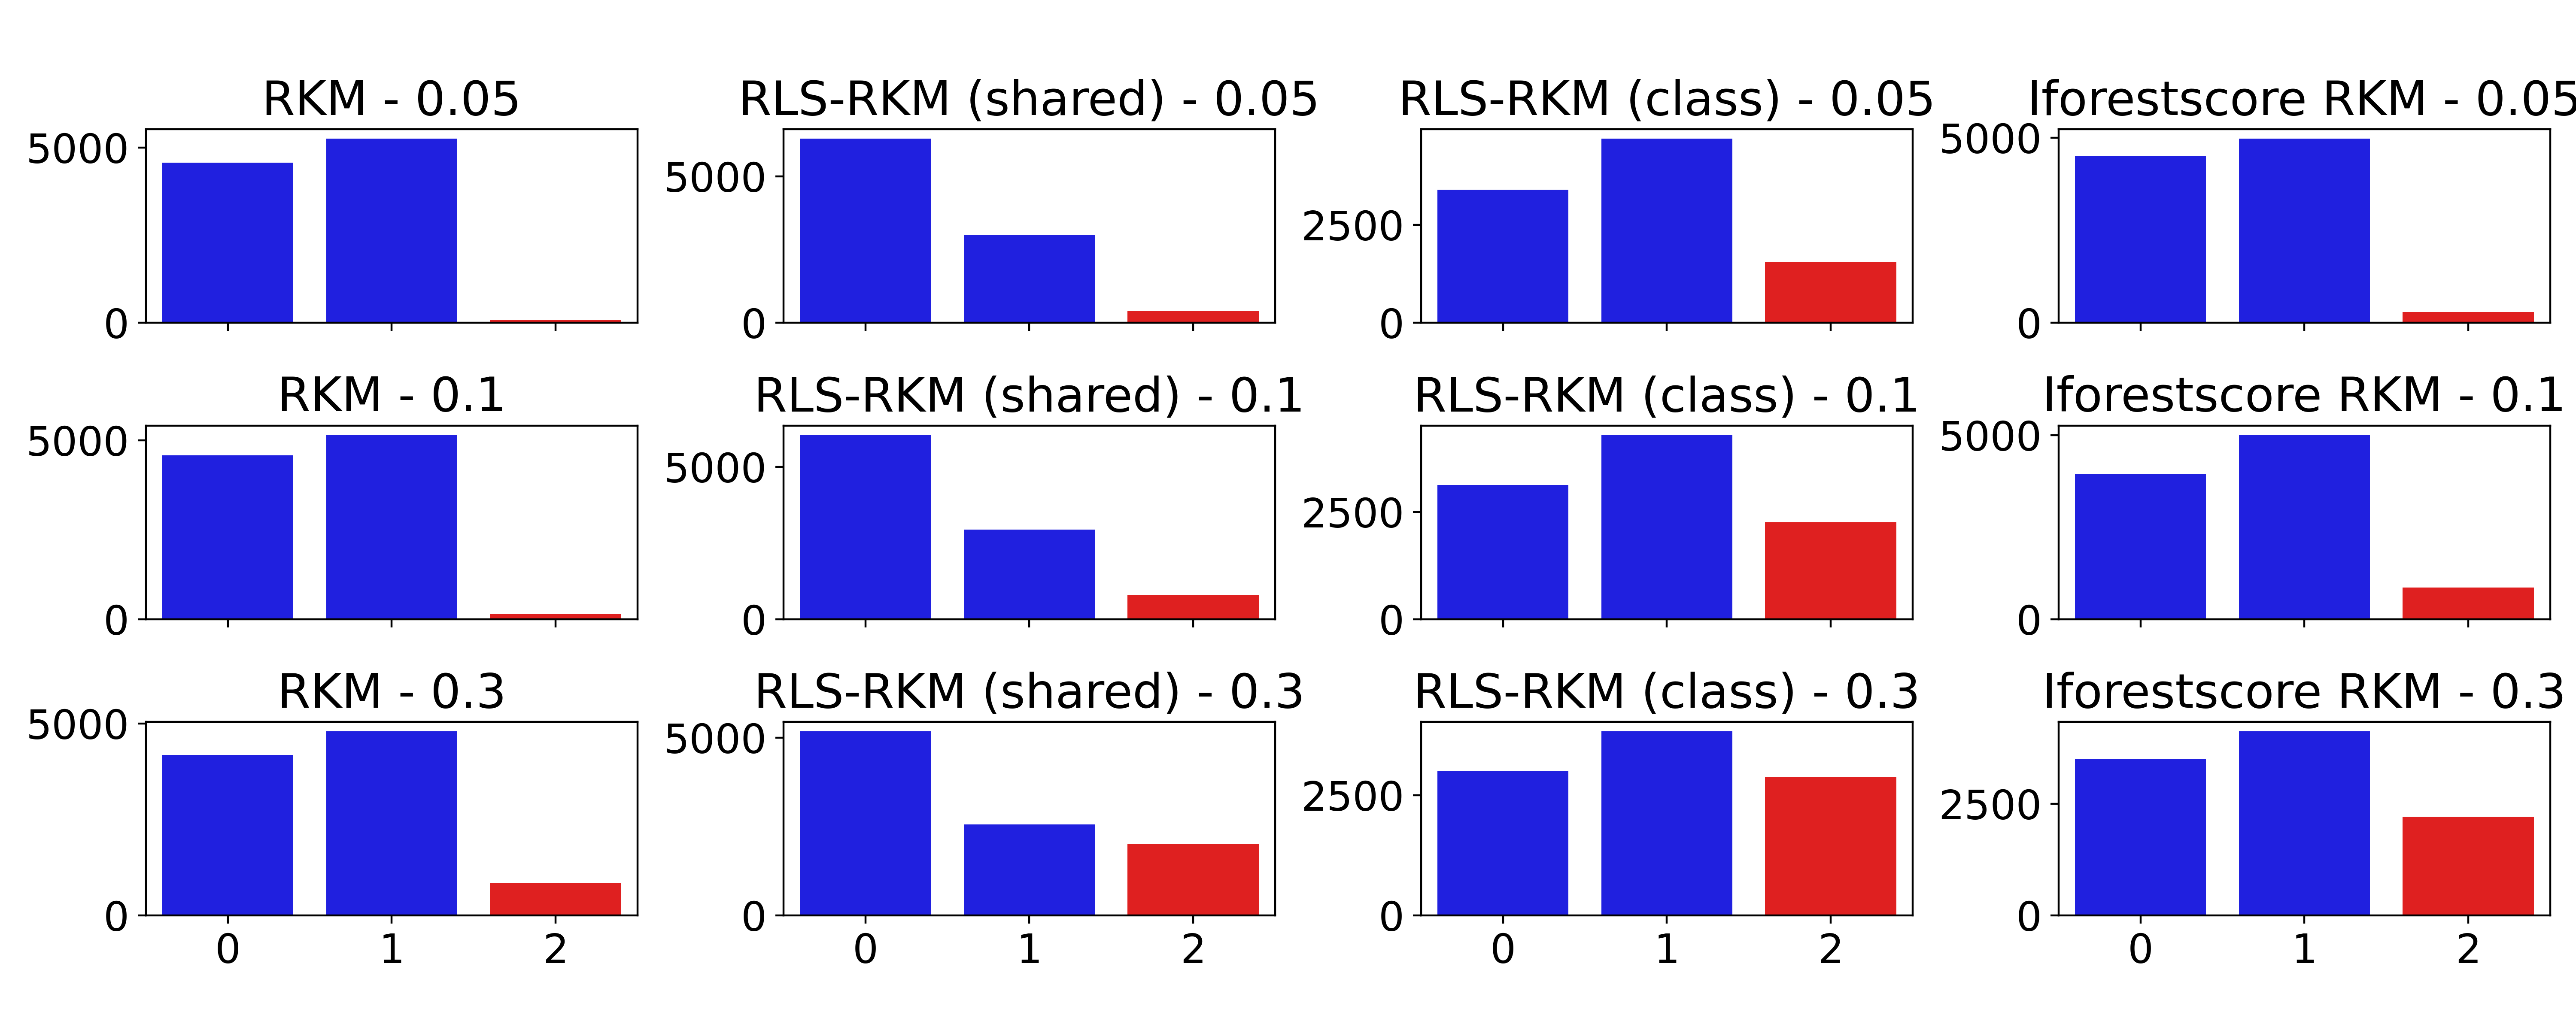
\includegraphics[width=\linewidth]{Figures/Methods/expr-mnist012-gen-dist.png}
%     \caption{Counts of generated samples per mode from different RKM models on unbalanced MNIST012 dataset.}
%     \label{fig-rls-gen-dist-ubmnist012}
% \end{figure}

% \begin{table}[ht]
    \centering
    \begin{tabular}{ccccc}
\toprule
\makecell{Imbalance \\ ratio} & Model & Minority mean & KL score ($\downarrow$) & FID ($\downarrow$) \\
\midrule
\multirow{4}{*}{0.05} & RKM & 113 (±13) & 0.49 (±0.02) & 39.19 (±1.17) \\
& RLS-RKM (shared) & 179 (±11) & 0.42 (±0.01) & 40.36 (±0.46) \\
& RLS-RKM (class) & \textbf{342} (±35) & \textbf{0.35} (±0.01) & \textbf{34.65} (±1.95) \\
& IforestRKM & 144 (±15) & 0.49 (±0.02) & 39.08 (±1.01) \\
\midrule
\multirow{4}{*}{0.10} & RKM & 185 (±11) & 0.40 (±0.01) & 38.89 (±0.18) \\
& RLS-RKM (shared) & 327 (±3) & \textbf{0.27} (±0.00) & 38.38 (±0.93) \\
& RLS-RKM (class) & \textbf{462} (±15) & \textbf{0.27} (±0.01) & \textbf{33.68} (±0.97) \\
& IforestRKM & 257 (±7) & 0.37 (±0.01) & 35.32 (±1.17) \\
\midrule
\multirow{4}{*}{0.30} & RKM & 478 (±14) & 0.15 (±0.01) & 34.09 (±1.28) \\
& RLS-RKM (shared) & 629 (±11) & \textbf{0.10} (±0.01) & 36.01 (±0.97) \\
& RLS-RKM (class) & \textbf{797} (±14) & 0.13 (±0.01) & \textbf{30.74} (±1.67) \\
& IforestRKM & 547 (±44) & 0.15 (±0.02) & 32.23 (±0.24) \\
\bottomrule
\end{tabular}
    \caption{Results of experiments on the unbalanced MNIST dataset under different imbalance ratios. Experiments are replicated over 3 runs with random initializations. Means and standard deviations (enclosed in parentheses) for each metric are reported. "Minority mean" refers to the average number of samples generated from each minority mode.
}
    \label{rls-expr-mnist}
\end{table}



% \begin{figure}[H]
%     \centering
%     \includegraphics[width=\linewidth]{Figures/Methods/expr-rls-mnist-gen-dist.png}
%     \caption{Counts of generated samples per mode from different RKM models on unbalanced MNIST012 dataset.}
%     \label{fig-rls-gen-dist-ubmnist}
% \end{figure}
% \section{Discussion}

\chapter{Conclusions}
\label{chap-conclu}
This thesis investigated various sampling techniques for training the Gen-RKM model in scenarios with unbalanced inputs. These sampling strategies aimed at increasing the diversity of the model's generation in an imbalanced input context. Depending on the availability of data labels, the experiments were carried out in both supervised and unsupervised settings. 

In the supervised learning context, unbalanced MNIST and unbalanced Fashion MNIST datasets have been specifically created to train the learning models. When comparing the results of inverse frequency sampling with the standard uniform sampling in Gen-RKM, it was obvious that inverse frequency sampling facilitated a more balanced generation of data and increased the generation of samples from minority classes during the training phase. Additionally, inverse frequency sampling demonstrated the capability to selectively generate samples from minority classes when integrated with conditional generation techniques in Gen-RKM.

In the unsupervised context, RLS sampling and Iforest score sampling have been tested and discussed on 2D synthetic datasets, 012-MNIST, MNIST, and FashionMNIST datasets, with each of them having been tested with different imbalance ratios and different feature maps. The results of the experiments indicated that both RLS sampling and Iforest score sampling showed noticeable improvement compared to vanilla Gen-RKM in the diversity of model generation. RLS sampling with implicit feature maps performs well for low-dimensional data. RLS sampling, particularly when using fixed explicit feature maps such as pre-trained classifiers, delivered outstanding outcomes in high-dimensional scenarios on datasets with a limited number of modes. For datasets consisting of a large number of modes, such as those containing 10 or 25 modes, RLS sampling still outperformed the baseline and other sampling strategies, even though the results were not as impressive as those achieved with simpler datasets. 

In addition, the risk of these over-sampling-based methods has been discussed, which provided insights for numerous future studies. We summarize the suggestions for future works as follows:
\begin{itemize}[label={--}]
    \item Instead of simply increasing the probability of sampling the minority, resampling the data in a more advanced way (e.g., applying differentiable augmentation for over-sampled data \cite{zhaoDifferentiableAugmentationDataEfficient2020}) to avoid the risk of data copying/over-fitting in the generation phase.
    \item As the performance of RLS sampling is particularly dependent on the choice of feature map, finding more advanced feature extractors is intriguing.
    \item Given the training of Gen-RKM with RLS sampling is quite computationally expensive, especially using shared feature maps, adaptions with faster RLS approximation schemes in the RKM framework are subject to future research.
    \item Currently, our work is limited to Gen-RKM framework. RLS sampling (or other possible weighted sampling schemes) could also be extended to Stiefel RKM\cite{pandeyDisentangledRepresentationLearning2022} in the future.
\end{itemize}



% At first, instead of simply increasing the probability of sampling the minority, resampling the data in a more advanced way to avoid the risk of data copying/over-fitting in the generation phase. Second, as the performance of RLS sampling is particularly dependent on the choice of feature map, finding more advanced feature extractors is intriguing. Lastly, given the training of Gen-RKM with RLS sampling is quite computationally expensive, especially using shared feature maps, further research into optimizing the algorithm to reduce computational demands is necessary.  \cleardoublepage
% BACK MATTER (is dit zelfs een woord?)

% BIBLIOGRAPHY
\addcontentsline{toc}{chapter}{Bibliography}
%\bibliographystyle{plain}
%\bibliography{Bibliography/references_wen.bib}
% \cleardoublepage
\printbibliography

% APPENDIX
\begin{appendices}
\addtocontents{toc}{\protect\setcounter{tocdepth}{1}}
  \chapter{Supplementary material for
Chapter \ref{chap-methods}}
\section{Derivation of the conditional distribution of GMM}
\label{A-conGMM}
Given that the latent variable $\bh$ and its corresponding label $\by$ (in the form of one-hot encoding). We assume that their joint PDF is modeled by a mixture of multivariate Gaussians:
\begin{equation}
    p(\bh,\by) = \sum_{k=1}^{l}\pi_{k}\Normal(\bh_{cat}|\bmu_{k},\bSigma_{k})
\end{equation}
where $\bh_{cat}$ is the concatenated vector of $\bh$ and $\by$. Recall that the conditionals or the marginals of a multivariate Gaussian results in another Gaussian distribution. More specifically, for a multivariate Gaussian distribution $p(\bx) = \Normal(\bx|\bu,\bSigma)$ with the following partition 
\begin{equation}
    \bx = \begin{pmatrix}
        \bx_a\\
        \bx_b
    \end{pmatrix},\quad
    \bmu = \begin{pmatrix}
        \bmu_a\\
        \bmu_b
    \end{pmatrix},\quad
    \bSigma = \begin{pmatrix}
        \bSigma_{aa} & \bSigma_{ab} \\
        \bSigma_{ba} & \bSigma_{bb} \\
    \end{pmatrix},
\end{equation}
the conditional distribution is given by
\begin{equation}
    p(\bx_a|\bx_b) = \Normal(\bx_a | \bmu_{a|b},\bSigma_{a|b}),
\end{equation}
where
\begin{equation}
    \begin{aligned}
         \bmu_{a|b} &= \bmu_a + \bSigma_{ab} \bSigma_{bb}^{-1} (\bx_b - \bmu_b) \\
    \bSigma_{a|b} &= \bSigma_{aa} - \bSigma_{ab} \bSigma_{bb}^{-1} \bSigma_{ba}.
    \end{aligned}
\end{equation}
As for the marginal, it is simply given by $p(\bx_a) = \Normal(\bx_a|\bmu_a,\bSigma_{aa})$.

Back to the setting of GMM, since conditional of each Gaussian is another Gaussian, the conditional distribution of $\bh$ given a certain class label is then characterized by another mixture of Gaussians:
\begin{equation}
    p(\bh | \by) = \sum_{k=1}^{l}\pi_k^{\prime}\Normal(\bh | \bmu_{\bh|\by,k},\bSigma_{\bh|\by,k}).
\end{equation}
To compute the updated weights $\pi_{k}^{\prime}$ for each component Gaussian, one needs to apply Bayes' rule:
\begin{equation}
    \begin{aligned}
        p(\bh | \by) &= \frac{p(\bh,\by)}{p(\by)} \\
        &= \sum_{k=1}^{l}\frac{\pi_k \Normal(\bh_{cat}|\bmu_k,\bSigma_k)}{p(\by)} \\
        &= \sum_{k=1}^{l} \frac{\pi_k\Normal(\by|\bmu_{c,k},\bSigma_{\by\by,k})\Normal(\bh | \bmu_{\bh|\by,k},\bSigma_{\bh|\by,k})}{p(\by)} \\
        &= \sum_{k=1}^{l}  \underbrace{\frac{\pi_k \Normal(\by|\bmu_{\by,k},\bSigma_{\by\by,k})}{\sum_{v=1}^{l}\pi_{v}\Normal(\by | \bmu_{\by,v},\bSigma_{\by\by,v})}}_{=\pi_{k}^{\prime}}\Normal(\bh | \bmu_{\bh|\by,k},\bSigma_{\bh|\by,k}).
    \end{aligned}
\end{equation}

\chapter{Additional results of
Chapter \ref{chap-expr}}

\section{Generated Samples: Comparison Between Vanilla Gen-RKM and Gen-RKM with RLS Sampling Adaptation}

\subsection{Unbalanced 012-MNIST}
\begin{figure}[H]
    \centering
    \begin{subfigure}{0.45\textwidth}
        \centering
        \includegraphics[width=0.8\textwidth]{Figures/Methods/rkm-mnist012-gensamples-highlighted-minorities.png}
    \end{subfigure}
    \hfill
    \begin{subfigure}{0.45\textwidth}
        \centering
        \includegraphics[width=0.8\textwidth]{Figures/Methods/RLS-mnist012-gensamples-highlighted-minorities.png}
    \end{subfigure}
    \caption{Generated images from the unbalanced 012-MNIST dataset by vanilla RKM (left) and RLS (class) sampling adapted RKM (right). Images are highlighted by a red border if classified as minority modes.}
    \label{fig-gensamples-ubmnist012-rls}
\end{figure}


\subsection{Unbalanced MNIST}

\begin{figure}[H]
    \centering
    \begin{subfigure}{0.45\textwidth}
        \centering
        \includegraphics[width=0.8\textwidth]{Figures/Methods/rkm-mnist-gensamples-highlighted-minorities.png}
    \end{subfigure}
    \hfill
    \begin{subfigure}{0.45\textwidth}
        \centering
        \includegraphics[width=0.8\textwidth]{Figures/Methods/RLS-mnist-gensamples-highlighted-minorities.png}
    \end{subfigure}
    \caption{Generated images from the unbalanced MNIST dataset by vanilla RKM (left) and RLS (class) sampling adapted RKM (right). Images are highlighted by a red border if classified as minority modes.}
    \label{fig-gensamples-ubmnist-rls}
\end{figure}


\subsection{Unbalanced Fashion MNIST}

\begin{figure}[H]
    \centering
    \begin{subfigure}{0.45\textwidth}
        \centering
        \includegraphics[width=0.8\textwidth]{Figures/Methods/rkm-fashion-gensamples-highlighted-minorities.png}
    \end{subfigure}
    \hfill
    \begin{subfigure}{0.45\textwidth}
        \centering
        \includegraphics[width=0.8\textwidth]{Figures/Methods/RLS-fashion-gensamples-highlighted-minorities.png}
    \end{subfigure}
    \caption{Generated images from the unbalanced Fashion MNIST dataset by vanilla RKM (left) and RLS (class) sampling adapted RKM (right). Images are highlighted by a red border if classified as minority modes.}
    \label{fig-gensamples-ubfashion-rls}
\end{figure}
\end{appendices}

% Back side of book
\cleartoleftpage{} % Make sure the back page is at an even page number


% ----------------------- Achterblad ------------------------------
% Vergeet niet de tekst aan te passen:
% - Afdeling
% - Adres van de afdeling
% - Telefoon en faxnummer
% -----------------------------------------------------------------
\thispagestyle{empty}
\sffamily
%
\begin{textblock}{191}(113,-11)
{\color{blueline}\rule{160pt}{5.5pt}}
\end{textblock}
%
\begin{textblock}{191}(168,-11)
{\color{blueline}\rule{5.5pt}{59pt}}
\end{textblock}
%
\begin{textblock}{183}(-24,-11)
\textblockcolour{}
\flushright
\fontsize{7}{7.5}\selectfont
\textbf{AFDELING}\\
Straat nr bus 0000\\
3000 LEUVEN, BELGI\"{E}\\
tel. + 32 16 00 00 00\\
fax + 32 16 00 00 00\\
www.kuleuven.be\\
\end{textblock}
%
\begin{textblock}{191}(154,-7)
\textblockcolour{}
\includegraphics*[height=16.5truemm]{Figures/sedes}
\end{textblock}
%
\begin{textblock}{191}(-20,235)
{\color{bluetitle}\rule{544pt}{55pt}}
\end{textblock}

\end{document}